% ======================================================================
% scrlttr2-de.tex
% Copyright (c) Markus Kohm, 2002-2023
%
% This file is part of the LaTeX2e KOMA-Script bundle.
%
% This work may be distributed and/or modified under the conditions of
% the LaTeX Project Public License, version 1.3c of the license.
% The latest version of this license is in
%   https://www.latex-project.org/lppl.txt
% and version 1.3c or later is part of all distributions of LaTeX 
% version 2005/12/01 or later and of this work.
%
% This work has the LPPL maintenance status "author-maintained".
%
% The Current Maintainer and author of this work is Markus Kohm.
%
% This work consists of all files listed in MANIFEST.md.
% ======================================================================
%
% Chapter about scrlttr2 of the KOMA-Script guide
% Maintained by Markus Kohm
%
% ============================================================================

\KOMAProvidesFile{scrlttr2-de.tex}%
                 [$Date: 2023-04-25 09:00:44 +0200 (Di, 25. Apr 2023) $
                  KOMA-Script guide (chapter: scrlttr2)]

\chapter{Briefe mit Klasse \Class{scrlttr2} oder Paket \Package{scrletter}}
\labelbase{scrlttr2}

\BeginIndexGroup
\BeginIndex{Class}{scrlttr2}\BeginIndex{Package}{scrletter}%
\BeginIndex{}{Briefe}%
\iffalse% Wird eigentlich nicht mehr als Einleitung benötigt
Briefe sind in vielerlei Hinsicht etwas ganz anderes als Artikel, Berichte,
Bücher oder Ähnliches. Schon allein deshalb gibt es für Briefe ein eigenes
Kapitel.%
\iffalse% Umbruchkorrektur
Aber auch aus weiteren Gründen ist ein eigenes Kapitel für
\Class{scrlttr2} und \Package{scrletter} gerechtfertigt.%
\fi%
\fi%

\iffalse% Braucht nach 17 Jahren kein Mensch mehr
Die Klasse \Class{scrlttr2}\important{\Class{scrlttr2}} wurde 2002 von Grund
auf neu entwickelt. Sie hat daher auch ein komplett anderes Bedienkonzept als
alle übrigen mir bekannten Klassen. Die neue Art der Bedienung ist
möglicherweise etwas ungewohnt, bietet jedoch nicht nur dem geübten Anwender
einige Vorteile.%
\fi%

Das Paket \Package{scrletter}\important{\Package{scrletter}}%
\ChangedAt{v3.15}{\Package{scrletter}} verstärkt \KOMAScript{} seit Version
3.15. Es stellt die auf Briefe ausgelegte Funktionalität von \Class{scrlttr2}
auch für andere Klassen bereit. Empfohlen wird die Verwendung mit einer der
\KOMAScript-Klassen \Class{scrbook}, \Class{scrreprt} oder \Class{scrartcl},
die im vorherigen Kapitel erklärt sind. %
\iffalse %
Mit geringfügigen Einschränkungen funktioniert \Package{scrletter}%
\else %
Auf Anwenderwunsch funktioniert \Package{scrletter} mit geringfügigen
Einschränkungen %
\fi %
aber auch mit den Standardklassen.

Ausgangspunkt für die Entwicklung von \Package{scrletter} waren
Nachfragen von Anwendern, die Elemente wie
Gliederungsüberschriften,\textnote{Überschriften, Gleitumgebungen,
  Verzeichnisse} Gleitumgebungen oder ein Literaturverzeichnis auch in Briefen
haben wollten. Umgekehrt gab es auch Wünsche nach der Verwendung der Variablen
von \Class{scrlttr2} in den übrigen \KOMAScript-Klassen. Beides ist durch eine
Kombination der gewünschten \KOMAScript-Klasse mit \Package{scrletter}
möglich.

Gegenüber der Briefklasse hat das Briefpaket einige, kleine Änderungen, die
notwendig waren, um Konflikte mit den anderen Klassen zu vermeiden. Diese
betreffen vor allem die Seitenstile und sind explizit dokumentiert (siehe
\autoref{sec:\LabelBase.pagestyle}, ab
\autopageref{sec:\LabelBase.pagestyle}). %
\iffalse % Umbruchkorrektur
Wo \Package{scrletter} nicht explizit erwähnt ist, gilt dafür alles, was für
\Class{scrlttr2} dokumentiert ist, ohne Änderung. %
\fi%

\LoadCommonFile{options} % \section{Frühe oder späte Optionenwahl}

\LoadCommonFile{compatibility} % \section{Kompatibilität zu früheren Versionen von \KOMAScript}

%\iffree{}{\vfill}% Umbruchoptimierung!

\LoadCommonFile{draftmode} % \section{Entwurfsmodus}

\LoadCommonFile{typearea} % \section{Seitenauf"|teilung}

Die Unterscheidung zwischen ein- und doppelseitigem Satz ist bei Briefen
jedoch in der Regel nicht sinnvoll. Da Briefe normalerweise nicht gebunden
werden, betrachtet man bei Briefen jede Seite für sich. Das gilt auch dann,
wenn ausnahmsweise Vorder- und Rückseite bedruckt werden. Daher spielt bei
Briefen normalerweise auch der vertikale Ausgleich keine Rolle. Sollten Sie
diesen trotzdem benötigen
\iffalse%
% Umbruchkorrekturtext
oder wissen wollen, was das ist, %
\fi%
sei auf die in \autoref{sec:maincls.typearea},
\DescPageRef{maincls.cmd.flushbottom} erklärten Anweisungen
\DescRef{maincls.cmd.raggedbottom}\IndexCmd{raggedbottom} und
\DescRef{maincls.cmd.flushbottom}\IndexCmd{flushbottom} verwiesen.%
%
\EndIndexGroup


\section{Variablen}
\seclabel{variables}%
\BeginIndexGroup
\BeginIndex{}{Variablen}%

Neben Optionen, Anweisungen (oder Befehlen), Umgebungen, Zählern und Längen
wurden in \autoref{cha:maincls} für \KOMAScript{} bereits zusätzlich Elemente
eingeführt.  Eine typische Eigenschaft eines Elements ist seine Schriftart und
die Möglichkeit, diese zu ändern (siehe \autoref{sec:\LabelBase.textmarkup},
\DescPageRef{\LabelBase.cmd.setkomafont}).  An dieser Stelle werden nun
zusätzlich Variablen eingeführt. Variablen haben einen
Namen\Index{Variablen>Name}\textnote{Namen}, über den sie angesprochen werden,
und einen Inhalt\Index{Variablen>Inhalt}\textnote{Inhalt}. Der Inhalt einer
Variablen kann zeitlich bzw. räumlich getrennt von ihrer Verwendung gesetzt
werden, so wie der Inhalt einer Anweisung getrennt von ihrer Ausführung
definiert werden kann. Hauptunterschied zwischen Variablen und Anweisungen
ist, dass Anweisungen üblicherweise Aktionen auslösen, während der Inhalt
einer Variablen normalerweise aus einem Text besteht, der dann von einer
Anweisung ausgegeben wird. Er kann aber auch von mehreren Anweisungen an
unterschiedlichen Stellen verwendet und so mehrfach ausgegeben
werden. Außerdem kann eine Variable zusätzlich eine
Bezeichnung\Index{Variablen>Bezeichnung}\textnote{Bezeichnung} besitzen, die
ebenfalls gesetzt und ausgegeben werden kann.

Dieser Abschnitt beschränkt sich bewusst auf die Einführung des Begriffs der
Variablen. Die zur Verdeutlichung verwendeten Beispiele sind ohne tiefere
Bedeutung. Konkretere Anwendungsbeispiele gibt es bei der Erläuterung der in
der Klasse und dem Paket bereits definierten und von ihnen verwendeten
Variablen in den nachfolgenden Abschnitten. \autoref{tab:\LabelBase.variables}
gibt eine Übersicht über alle definierten Variablen.
%
\begin{desclist}
  \desccaption{Von \Class{scrlttr2} und \Package{scrletter} unterstützte
    Variablen\label{tab:\LabelBase.variables}}%
  {Von \Class{scrlttr2} und \Package{scrletter} unterstützte Variablen
    (\emph{Fortsetzung})}%
  \ventry{addresseeimage}{Anweisungen, die zum Setzen
    des Port-Payé-Kopfes bei der Einstellung
    \OptionValueRef{\LabelBase}{addrfield}{backgroundimage} oder der
    Port-Payé-Anschrift bei der Einstellung
    \OptionValueRef{\LabelBase}{addrfield}{image}, verwendet werden
    (\autoref{sec:\LabelBase.firstpage},
    \DescPageRef{\LabelBase.variable.addresseeimage})}%
  \ventry{backaddress}{Rücksendeadresse für Fensterbriefumschläge
    (\autoref{sec:\LabelBase.firstpage},
    \DescPageRef{\LabelBase.variable.backaddress})}%
  \ventry{backaddressseparator}{Trennzeichen innerhalb der Rücksendeadresse
    (\autoref{sec:\LabelBase.firstpage},
    \DescPageRef{\LabelBase.variable.backaddressseparator})}%
  \ventry{ccseparator}{Trennzeichen zwischen Verteilertitel und Verteiler
    (\autoref{sec:\LabelBase.document},
    \DescPageRef{\LabelBase.variable.ccseparator})}%
  \ventry{customer}{Geschäftszeilenfeld »Kundennummer«
    (\autoref{sec:\LabelBase.firstpage},
    \DescPageRef{\LabelBase.variable.customer})}%
  \ventry{date}{Datum (\autoref{sec:\LabelBase.firstpage},
    \DescPageRef{\LabelBase.variable.date})}%
  \ventry{emailseparator}{Trennzeichen zwischen E-Mail-Bezeichnung und
    E-Mail-Adresse (\autoref{sec:\LabelBase.firstpage},
    \DescPageRef{\LabelBase.variable.emailseparator})}%
  \ventry{enclseparator}{Trennzeichen zwischen Anlagetitel und Anlagen
    (\autoref{sec:\LabelBase.document},
    \DescPageRef{\LabelBase.variable.enclseparator})}%
  \ventry{faxseparator}{Trennzeichen zwischen Faxbezeichner und Faxnummer
    (\autoref{sec:\LabelBase.firstpage},
    \DescPageRef{\LabelBase.variable.faxseparator})}%
  \ventry{firstfoot}{%
    Seitenfuß\ChangedAt{v3.08}{\Class{scrlttr2}} des Briefbogens
    (\autoref{sec:\LabelBase.firstpage},
    \DescPageRef{\LabelBase.variable.firstfoot})}%
  \ventry{firsthead}{%
    Kopf\ChangedAt{v3.08}{\Class{scrlttr2}} des Briefbogens
    (\autoref{sec:\LabelBase.firstpage},
    \DescPageRef{\LabelBase.variable.firsthead})}%
  \ventry{fromaddress}{Absenderadresse ohne Absendername
    (\autoref{sec:\LabelBase.firstpage},
    \DescPageRef{\LabelBase.variable.fromaddress})}%
  \ventry{frombank}{Bankverbindung des Absenders
    (\autoref{sec:\LabelBase.firstpage},
    \DescPageRef{\LabelBase.variable.frombank})}%
  \ventry{fromemail}{E-Mail-Adresse des Absenders
    (\autoref{sec:\LabelBase.firstpage},
    \DescPageRef{\LabelBase.variable.fromemail})}%
  \ventry{fromfax}{Faxnummer des Absenders
    (\autoref{sec:\LabelBase.firstpage},
    \DescPageRef{\LabelBase.variable.fromfax})}%
  \ventry{fromlogo}{Anweisungen zum Setzen des Absenderlogos
    (\autoref{sec:\LabelBase.firstpage},
    \DescPageRef{\LabelBase.variable.fromlogo})}%
  \ventry{frommobilephone}{%
    \ChangedAt{v3.12}{\Class{scrlttr2}}%
    Handynummer des Absenders (\autoref{sec:\LabelBase.firstpage},
    \DescPageRef{\LabelBase.variable.frommobilephone})}%
  \ventry{fromname}{vollständiger Absendername
    (\autoref{sec:\LabelBase.firstpage},
    \DescPageRef{\LabelBase.variable.fromname})}%
  \ventry{fromphone}{Telefonnummer des Absenders
    (\autoref{sec:\LabelBase.firstpage},
    \DescPageRef{\LabelBase.variable.fromphone})}%
  \ventry{fromurl}{eine URL des Absenders (\autoref{sec:\LabelBase.firstpage},
    \DescPageRef{\LabelBase.variable.fromurl})}%
  \ventry{fromzipcode}{Postleitzahl des Absenders für den Port-Payé-Kopf bei
    \OptionValueRef{\LabelBase}{addrfield}{PP}
    (\autoref{sec:\LabelBase.firstpage},
    \DescPageRef{\LabelBase.variable.fromzipcode})}%
  \ventry{invoice}{Geschäftszeilenfeld »Rechnungsnummer«
    (\autoref{sec:\LabelBase.firstpage},
    \DescPageRef{\LabelBase.variable.invoice})}%
  \ventry{location}{erweiterte Absenderangabe
    (\autoref{sec:\LabelBase.firstpage},
    \DescPageRef{\LabelBase.variable.location})}%
  \ventry{mobilephoneseparator}{Trennzeichen zwischen Handybezeichner und
    Handynummer (\autoref{sec:\LabelBase.firstpage},
    \DescPageRef{\LabelBase.variable.mobilephoneseparator})}%
  \ventry{myref}{Geschäftszeilenfeld »Mein Zeichen«
    (\autoref{sec:\LabelBase.firstpage},
    \DescPageRef{\LabelBase.variable.myref})}%
  \ventry{nextfoot}{Seitenfuß\ChangedAt{v3.08}{\Class{scrlttr2}} im Seitenstil
    \DescRef{\LabelBase.pagestyle.headings}\IndexPagestyle{headings} oder
    \DescRef{\LabelBase.pagestyle.myheadings}\IndexPagestyle{myheadings}
    (\autoref{sec:\LabelBase.pagestyle},
    \DescPageRef{\LabelBase.variable.nextfoot})}%
  \ventry{nexthead}{Kopf\ChangedAt{v3.08}{\Class{scrlttr2}} im Seitenstil
    \DescRef{\LabelBase.pagestyle.headings}\IndexPagestyle{headings} oder
    \DescRef{\LabelBase.pagestyle.myheadings}\IndexPagestyle{myheadings}
    (\autoref{sec:\LabelBase.pagestyle},
    \DescPageRef{\LabelBase.variable.nexthead})}%
  \ventry{phoneseparator}{Trennzeichen zwischen Telefonbezeichner und
    Telefonnummer (\autoref{sec:\LabelBase.firstpage},
    \DescPageRef{\LabelBase.variable.phoneseparator})}%
  \ventry{place}{Ort (\autoref{sec:\LabelBase.firstpage},
    \DescPageRef{\LabelBase.variable.place})}%
  \ventry{placeseparator}{Trennzeichen zwischen Ort und Datum
    (\autoref{sec:\LabelBase.firstpage},
    \DescPageRef{\LabelBase.variable.placeseparator})}%
  \ventry{PPdatamatrix}{Anweisungen zum Setzen einer Data-Matrix bei der
    Einstellung \OptionValueRef{\LabelBase}{addrfield}{PP}
    (\autoref{sec:\LabelBase.firstpage},
    \DescPageRef{\LabelBase.variable.PPdatamatrix})}%
  \ventry{PPcode}{Code zur Identifizierung des Absenders bei Einstellung
    \OptionValueRef{\LabelBase}{addrfield}{PP}
    (\autoref{sec:\LabelBase.firstpage},
    \DescPageRef{\LabelBase.variable.PPcode})}%
  \ventry{signature}{Signatur unter Unterschrift und Grußformel
    (\autoref{sec:\LabelBase.closing},
    \DescPageRef{\LabelBase.variable.signature})}%
  \ventry{specialmail}{Versandart (\autoref{sec:\LabelBase.firstpage},
    \DescPageRef{\LabelBase.variable.specialmail})}%
  \ventry{subject}{Betreff (\autoref{sec:\LabelBase.firstpage},
    \DescPageRef{\LabelBase.variable.subject})}%
  \ventry{subjectseparator}{Trennzeichen zwischen Betreff"|titel und Betreff
    (\autoref{sec:\LabelBase.firstpage},
    \DescPageRef{\LabelBase.variable.subjectseparator})}%
  \ventry{title}{Brief"|titel (\autoref{sec:\LabelBase.firstpage},
    \DescPageRef{\LabelBase.variable.title})}%
  \ventry{toaddress}{Empfängeradresse ohne Empfängername
    (\autoref{sec:\LabelBase.firstpage},
    \DescPageRef{\LabelBase.variable.toaddress})}%
  \ventry{toname}{vollständiger Empfängername
    (\autoref{sec:\LabelBase.firstpage},
    \DescPageRef{\LabelBase.variable.toname})}%
  \ventry{yourmail}{Geschäftszeilenfeld »Ihr Schreiben«
    (\autoref{sec:\LabelBase.firstpage},
    \DescPageRef{\LabelBase.variable.yourmail})}%
  \ventry{yourref}{Geschäftszeilenfeld »Ihr Zeichen«
    (\autoref{sec:\LabelBase.firstpage},
    \DescPageRef{\LabelBase.variable.yourref})}%
  \ventry{zipcodeseparator}{Trennzeichen zwischen der Bezeichnung und dem
    Inhalt der Variablen \DescRef{\LabelBase.variable.fromzipcode}
    (\autoref{sec:\LabelBase.firstpage},
    \DescPageRef{\LabelBase.variable.zipcodeseparator})}%
\end{desclist}


\begin{Declaration}
  \Macro{setkomavar}
    \Parameter{Name}\OParameter{Bezeichnung}\Parameter{Inhalt}
  \Macro{setkomavar*}\Parameter{Name}\Parameter{Bezeichnung}
\end{Declaration}
Mit der Anweisung \Macro{setkomavar} wird der \PName{Inhalt} der Variablen
\PName{Name} gesetzt. Dabei kann per optionalem Argument gleichzeitig auch die
\PName{Bezeichnung} der Variablen mit geändert werden. Mit der
Sternvariante \Macro{setkomavar*} kann auch nur die \PName{Bezeichnung} der
Variablen \PName{Name} gesetzt werden.
\begin{Example}
  In Briefen ist es üblich, den Absender im Briefkopf stehen zu haben. Dazu
  muss \KOMAScript{} den Absender aber erst einmal mit Namen kennen. Für
  »Peter Musterfrau« ginge das einfach mit:
\begin{lstcode}
  \setkomavar{fromname}{Peter Musterfrau}
\end{lstcode}
  Die voreingestellte Bezeichnung für den Namen des Absenders ist
  »Von«. Angenommen, Herr Musterfrau will %
  \iffalse aber \fi % Umbruchkorrektur
  an den Stellen, an denen \KOMAScript{} diese Bezeichnung verwendet, lieber
  »Absender« haben, so müsste er zusätzlich
\begin{lstcode}
  \setkomavar*{fromname}{Absender}
\end{lstcode}
  setzen oder aber die beiden Angaben zu einer Anweisung zusammenfassen:
\begin{lstcode}
  \setkomavar{fromname}[Absender]{Peter Musterfrau}
\end{lstcode}
  Damit schlägt er sozusagen zwei Fliegen mit einer Klappe.
\end{Example}
Übrigens kann mit einem leeren obligatorischen Argument \PName{Inhalt}
der Inhalt der Variable gelöscht werden. Selbstverständlich kann in
gleicher Weise mit einem leeren Argument \PName{Bezeichnung} auch die
Bezeichnung der Variablen gelöscht werden.
\begin{Example}
  Angenommen, Herr Musterfrau will gar keine Bezeichnung für den Namen des
  Absenders haben. Dann könnte er diese entweder für sich mit:
\begin{lstcode}
  \setkomavar*{fromname}{}
\end{lstcode}
  löschen. Er könnte aber auch wieder zwei Fliegen mit einer Klappe
  schlagen und
\begin{lstcode}
  \setkomavar{fromname}[]{Peter Musterfrau}
\end{lstcode}
  verwenden. Dadurch wird gleichzeitig der Inhalt der Variablen gesetzt und
  ihre Bezeichnung gelöscht.%
\end{Example}%
\iftrue% Umbruchkorrektur
Ein\textnote{Achtung!} leeres optionales Argument ist also nicht
gleichbedeutend mit dem Weglassen des optionalen Arguments.%
\else %
\vskip -1\ht\strutbox plus .75\strutbox% Beispiel am Ende der Bechreibung
\fi%
\EndIndexGroup

\begin{Declaration}
  \Macro{usekomavar}\OParameter{Anweisung}\Parameter{Name}
  \Macro{usekomavar*}\OParameter{Anweisung}\Parameter{Name}
\end{Declaration}
In\ChangedAt{v2.9i}{\Class{scrlttr2}} manchen Fällen wird es notwendig sein,
selbst auf den Inhalt oder die Bezeichnung einer Variablen zuzugreifen, dies
also nicht allein der Klasse zu überlassen. Das gilt insbesondere dann, wenn
Sie eigene Variablen definiert haben, die nicht zur Geschäftszeile
hinzugefügt werden.  Mit der Anweisung \Macro{usekomavar} können Sie auf den
Inhalt der Variablen \PName{Name} zugreifen, während Sie mit der Sternvariante
\Macro{usekomavar*} ihre Bezeichnung erhalten. Näheres zur Definition eigener
Variablen ist \autoref{sec:scrlttr2-experts.variables},
\DescPageRef{scrlttr2-experts.cmd.newkomavar} zu entnehmen.%
\EndIndexGroup


\begin{Declaration}
  \Macro{Ifkomavar}\Parameter{Name}\Parameter{Dann-Teil}\Parameter{Sonst-Teil}
\end{Declaration}
Mit\ChangedAt{v3.03}{\Class{scrlttr2}}%
\ChangedAt{v3.28}{\Class{scrlttr2}\and \Package{scrletter}} dieser Anweisung
kann man feststellen, ob eine Variable definiert ist. Der \PName{Dann-Teil}
wird nur dann ausgeführt, wenn die Variable existiert. Dabei wird der Inhalt
der Variablen nicht getestet, kann also auch leer sein. Der \PName{Sonst-Teil}
wird hingegen ausgeführt, wenn die Variable nicht existiert. Solche Tests
können beispielsweise dann sinnvoll sein, wenn eigene Variablen in einer
\File{lco}-Datei\Index{lco-Datei=\File{lco}-Datei} (siehe
\autoref{sec:\LabelBase.lcoFile} ab \autopageref{sec:\LabelBase.lcoFile})
definiert werden und in einer anderen \File{lco}-Datei diese Variable nur dann
verwendet werden soll, wenn sie existiert.  \EndIndexGroup


\begin{Declaration}
  \Macro{Ifkomavarempty}
    \Parameter{Name}\Parameter{Dann-Teil}\Parameter{Sonst-Teil}
  \Macro{Ifkomavarempty*}
    \Parameter{Name}\Parameter{Dann-Teil}\Parameter{Sonst-Teil}
\end{Declaration}
Mit\ChangedAt{v2.9i}{\Class{scrlttr2}}%
\ChangedAt{v3.28}{\Class{scrlttr2}\and \Package{scrletter}} Hilfe dieser
Anweisungen kann man feststellen, ob der Inhalt oder die Bezeichnung einer
Variablen leer ist oder nicht. Der \PName{Dann-Teil} wird nur dann ausgeführt,
wenn der expandierte Inhalt oder die expandierte Bezeichnung der Variablen
\PName{Name} leer ist. Anderenfalls wird der \PName{Sonst-Teil} ausgeführt.
Die Sternvariante der Anweisung bezieht sich dabei auf die Bezeichnung der
Variablen, während die normale Variante den Inhalt behandelt.%
\EndIndexGroup
%
\EndIndexGroup


\section{Pseudolängen}
\seclabel{pseudoLength}
\BeginIndexGroup
\BeginIndex{}{Pseudolängen}

Längen werden bei \LaTeX{} mit den drei Anweisungen
\Macro{newlength}\IndexCmd{newlength}, \Macro{setlength}\IndexCmd{setlength}
und \Macro{addtolength}\IndexCmd{addtolength} verarbeitet. Sehr viele Pakete
nutzen aber auch Makros, also Anweisungen, um Längen zu
speichern. \KOMAScript{} erweitert dieses Verfahren um die Möglichkeit, solche
in Makros gespeicherten Längen mit ähnlichen Anweisungen zu verarbeiten wie
echte Längen. Diese eigentlich in Makros abgelegten Längen heißen bei
\KOMAScript{} daher Pseudolängen.

Bitte beachten\textnote{Achtung!} Sie unbedingt, dass die Pseudolängen zwar
intern als Makros implementiert sind, bei den Befehlen zur Nutzung der
Pseudolängen jedoch nur die Namen anzugeben sind. Diese werden wie die Namen
von \LaTeX-Zählern und im Gegensatz zu Makros oder echten Längen ohne
umgekehrten Schrägstrich geschrieben!

\begin{Explain}
  Historisch gesehen arbeitet \TeX{} mit einem festen Satz an Registern. Es
  gibt jeweils 256~Register für Token, Boxen, Zähler, Abstände (englisch:
  \emph{skip}) und Größen (englisch: \emph{dimension}). Für \LaTeX{}-Längen,
  die mit \Macro{newlength} angefordert werden, werden Abstandsregister
  belegt. Sind alle diese Register verbraucht, kann man keine weiteren Längen
  definieren. Sowohl \Class{scrlttr2} als auch \Package{scrletter} würden
  normalerweise allein für die erste Seite mehr als 20 solche Register
  verbrauchen. \LaTeX{} selbst belegt bereits 40 dieser Register. Das
  \hyperref[cha:typearea]{\Package{typearea}}%
  \IndexPackage{typearea}-Paket benötigt ebenfalls einige, so dass ein Viertel
  der kostbaren Register verbraucht wäre. Dies war 2002 der Hauptgrund für die
  Einführung der Pseudolängen bei \Class{scrlttr2}.

  Wer nun einwenden will, dass \LaTeX{} in der empfohlenen und für
  \KOMAScript{} benötigten Installation mit \eTeX{} inzwischen das oben
  genannte Beschränkungsproblem nicht mehr besitzt, hat recht. Allerdings kam
  diese Entscheidung für \Class{scrlttr2} ein wenig zu spät. Bei
  \Package{scrletter} wurde das Konzept der Pseudolängen aus Gründen der
  Kompatibilität übernommen.
\end{Explain}

Eine Auf"|listung aller von \KOMAScript{} definierten und verwendeten
Pseudolängen ist \autoref{tab:\LabelBase.pseudoLengths} zu
entnehmen. Dabei ist auch angegeben, wo in den nachfolgenden Abschnitten
nähere Erklärungen zu der jeweiligen Pseudolänge zu finden
sind.%

\autoref{fig:\LabelBase.pseudoLengths} auf
\autopageref{fig:\LabelBase.pseudoLengths} zeigt eine schematische
Darstellung der wichtigsten Abstände auf dem Briefbogen. Dabei sind neben den
Pseudolängen für die veränderbaren Abstände zusätzlich in heller Schrift
die Längen angegeben, die für einige wenige fest programmierte Abstände
verwendet werden. Aus Gründen der Übersichtlichkeit wurde in der Darstellung
auf einige weniger häufig benötigte Pseudolängen jedoch verzichtet.
%
\begin{desclist}
  \renewcommand{\abovecaptionskipcorrection}{-\normalbaselineskip}%
  \desccaption{%
    Von \Class{scrlttr2} und \Package{scrletter} verwendete Pseudolängen%
    \label{tab:\LabelBase.pseudoLengths}%
  }{%
    Von \Class{scrlttr2} und \Package{scrletter} verwendete Pseudolängen
    (\emph{Fortsetzung})%
  }%
  \pentry{backaddrheight}{%
    Höhe der Rücksendeadresse am oberen Rand des Anschriftfeldes
    (\autoref{sec:\LabelBase.addressee},
    \DescPageRef{\LabelBase.plength.backaddrheight})%
  }%
  \pentry{bfoldmarklength}{%
    Länge der unteren horizontalen Faltmarke
    (\autoref{sec:\LabelBase.foldmarks},
    \DescPageRef{\LabelBase.plength.bfoldmarkvpos})%
  }%
  \pentry{bfoldmarkvpos}{%
    Abstand der unteren horizontalen Faltmarke von der oberen Kante des
    Papiers (\autoref{sec:\LabelBase.foldmarks},
    \DescPageRef{\LabelBase.plength.bfoldmarkvpos})%
  }%
  \pentry{firstfoothpos}{%
    Abstand des Brief"|fußes von der linken Kante des Papiers; Werte größer
    der Breite oder kleiner der negativen Breite des Papiers werden gesondert
    behandelt (\autoref{sec:\LabelBase.firstFoot},
    \DescPageRef{\LabelBase.plength.firstfoothpos})%|
  }%
  \pentry{firstfootvpos}{%
    Abstand des Brief"|fußes von der oberen Kante des Papiers
    (\autoref{sec:\LabelBase.firstFoot},
    \DescPageRef{\LabelBase.plength.firstfootvpos})%|
  }%
  \pentry{firstfootwidth}{%
    Breite des Brief"|fußes (\autoref{sec:\LabelBase.firstFoot},
    \DescPageRef{\LabelBase.plength.firstfootwidth})%|
  }%
  \pentry{firstheadhpos}{%
    Abstand des Briefkopfes von der linken Kante des Papiers; Werte größer der
    Breite oder kleiner der negativen Breite des Papiers werden gesondert
    behandelt (\autoref{sec:\LabelBase.firstHead},
    \DescPageRef{\LabelBase.plength.firstheadhpos})%
  }%\iffree{}{\enlargethispage*{\baselineskip}}% Umbruchkorrektur!!!
  \pentry{firstheadvpos}{%
    Abstand des Briefkopfes von der oberen Kante des Papiers
    (\autoref{sec:\LabelBase.firstHead},
    \DescPageRef{\LabelBase.plength.firstheadvpos})%
  }%
  \pentry{firstheadwidth}{%
    Breite des Briefkopfes (\autoref{sec:\LabelBase.firstHead},
    \DescPageRef{\LabelBase.plength.firstheadwidth})%
  }%
  \pentry{foldmarkhpos}{%
    Abstand der horizontalen Faltmarken von der linken Kante des Papiers
    (\autoref{sec:\LabelBase.foldmarks},
    \DescPageRef{\LabelBase.plength.foldmarkhpos})%
  }%
  \pentry{foldmarkvpos}{%
    Abstand der vertikalen Faltmarken von der oberen Kante des Papiers
    (\autoref{sec:\LabelBase.foldmarks},
    \DescPageRef{\LabelBase.plength.foldmarkvpos})%
  }%
  \pentry{fromrulethickness}{%
    Dicke einer optionalen \iftrue horizontalen \fi% Umbruchkorrektur
    Linie im Briefkopf (\autoref{sec:\LabelBase.firstHead},
    \DescPageRef{\LabelBase.plength.fromrulethickness})%
  }%
  \pentry{fromrulewidth}{%
    Länge einer optionalen \iftrue horizontalen \fi% Umbruchkorrektur
    Linie im Briefkopf (\autoref{sec:\LabelBase.firstHead},
    \DescPageRef{\LabelBase.plength.fromrulewidth})%
  }%
  \pentry{lfoldmarkhpos}{%
    Abstand der vertikalen Faltmarke von der linken Kante des Papiers
    (\autoref{sec:\LabelBase.foldmarks},
    \DescPageRef{\LabelBase.plength.lfoldmarkhpos})%
  }%
  \pentry{lfoldmarklength}{%
    Länge der vertikalen Faltmarke (\autoref{sec:\LabelBase.foldmarks},
    \DescPageRef{\LabelBase.plength.lfoldmarklength})%
  }%
  \pentry{locheight}{%
    Höhe der Absenderergänzung, falls der Wert nicht 0 ist; bei 0 wird
    stattdessen \DescRef{\LabelBase.plength.toaddrheight} verwendet
    (\autoref{sec:\LabelBase.locationField},
    \DescPageRef{\LabelBase.plength.locheight})%
  }%
  \pentry{lochpos}{%
    Abstand der Absenderergänzung von der rechten Papierkante, falls der Wert
    positiv ist, oder negativer Abstand der Absenderergänzung von der linken
    Papierkante, falls der Wert negativ ist; bei 0 wird stattdessen der
    negative Wert von \DescRef{\LabelBase.plength.toaddrhpos} verwendet
    (\autoref{sec:\LabelBase.locationField},
    \DescPageRef{\LabelBase.plength.lochpos})%
  }%
  \pentry{locvpos}{%
    Abstand der Absenderergänzung von der oberen Papierkante, falls der Wert
    nicht 0 ist; bei 0 wird stattdessen
    \DescRef{\LabelBase.plength.toaddrvpos} verwendet
    (\autoref{sec:\LabelBase.locationField},
    \DescPageRef{\LabelBase.plength.locvpos})%
  }%
  \pentry{locwidth}{%
    Breite des Feldes für die Absenderergänzung, wobei bei einem Wert von 0
    die Breite automatisch aufgrund der in \autoref{sec:\LabelBase.firstpage},
    \DescPageRef{\LabelBase.option.locfield} beschriebenen Option
    \DescRef{\LabelBase.option.locfield} berechnet wird
    (\autoref{sec:\LabelBase.locationField},
    \DescPageRef{\LabelBase.plength.locwidth})%
  }%\iffree{}{\enlargethispage*{\baselineskip}}% Umbruchkorrektur!!!%
  \pentry{mfoldmarklength}{%
    Länge der mittleren horizontalen Faltmarke
    (\autoref{sec:\LabelBase.foldmarks},
    \DescPageRef{\LabelBase.plength.mfoldmarklength})%
  }%
  \pentry{mfoldmarkvpos}{%
    Abstand der mittleren horizontalen Faltmarke von der oberen Kante des
    Papiers (\autoref{sec:\LabelBase.foldmarks},
    \DescPageRef{\LabelBase.plength.mfoldmarkvpos})%
  }%
  \pentry{pfoldmarklength}{%
    Länge der Lochermarke (\autoref{sec:\LabelBase.foldmarks},
    \DescPageRef{\LabelBase.plength.pfoldmarklength})%
  }%
  \pentry{PPdatamatrixvskip}{%
    vertikaler Abstand zwischen Port-Payé-Kopf und Data-Matrix bei
    \OptionValueRef{scrlttr2}{addrfield}{PP}
    (\autoref{sec:\LabelBase.addressee},
    \DescPageRef{\LabelBase.plength.PPdatamatrixvskip})%
  }%
  \pentry{PPheadheight}{%
    Höhe für den Port-Payé-Kopf (\autoref{sec:\LabelBase.addressee},
    \DescPageRef{\LabelBase.plength.PPheadheight})%
  }%
  \pentry{PPheadwidth}{%
    Breite des linken Port-Payé-Feldes bei
    \OptionValueRef{scrlttr2}{addrfield}{PP}
    (\autoref{sec:\LabelBase.addressee},
    \DescPageRef{\LabelBase.plength.PPheadwidth})%
  }%
  \pentry{refaftervskip}{%
    vertikaler Abstand nach der Geschäftszeile
    (\autoref{sec:\LabelBase.refLine},
    \DescPageRef{\LabelBase.plength.refaftervskip})%
  }%
  \pentry{refhpos}{%
    Abstand der Geschäftszeile von der linken Papierkante, wobei bei einem
    Wert von 0 automatisch relativ zur Papierbreite zentriert wird
    (\autoref{sec:\LabelBase.refLine},
    \DescPageRef{\LabelBase.plength.refhpos})%
  }%
  \pentry{refvpos}{%
    Abstand der Geschäftszeile von der oberen Kante des Papiers
    (\autoref{sec:\LabelBase.refLine},
    \DescPageRef{\LabelBase.plength.refvpos})%
  }%
  \pentry{refwidth}{%
    Breite der Geschäftszeile (\autoref{sec:\LabelBase.refLine},
    \DescPageRef{\LabelBase.plength.refwidth})%
  }%
  \pentry{sigbeforevskip}{%
    vertikaler Abstand zwischen Gruß und Signatur
    (\autoref{sec:\LabelBase.closing},
    \DescPageRef{\LabelBase.plength.sigbeforevskip})%
  }%
  \pentry{sigindent}{%
    Einzug der Signatur gegenüber dem Textkörper
    (\autoref{sec:\LabelBase.closing},
    \DescPageRef{\LabelBase.plength.sigindent})%
  }%
  \pentry{specialmailindent}{%
    linker Einzug der Versandart innerhalb des Anschriftfeldes
    (\autoref{sec:\LabelBase.addressee},
    \DescPageRef{\LabelBase.plength.specialmailindent})%
  }%
  \pentry{specialmailrightindent}{%
    rechter Einzug der Versandart innerhalb des Anschriftfeldes
    (\autoref{sec:\LabelBase.addressee},
    \DescPageRef{\LabelBase.plength.specialmailrightindent})%
  }%
  \pentry{subjectaftervskip}{%
    vertikaler Abstand nach dem Betreff (\autoref{sec:\LabelBase.subject},
    \DescPageRef{\LabelBase.plength.subjectaftervskip})%
  }%
  \pentry{subjectbeforevskip}{%
    zusätzlicher vertikaler Abstand vor dem Betreff
    (\autoref{sec:\LabelBase.subject},
    \DescPageRef{\LabelBase.plength.subjectbeforevskip})%
  }%
  \pentry{subjectvpos}{%
    Abstand des Betreffs von der oberen Kante des Papiers, wobei ein Wert von
    0 stattdessen den Betreff gemäß Option \DescRef{\LabelBase.option.subject}
    setzt (\autoref{sec:\LabelBase.subject},
    \DescPageRef{\LabelBase.plength.subjectaftervskip})%
  }%
  \pentry{tfoldmarklength}{%
    Länge der oberen horizontalen Faltmarke
    (\autoref{sec:\LabelBase.foldmarks},
    \DescPageRef{\LabelBase.plength.tfoldmarklength})%
  }%
  \pentry{tfoldmarkvpos}{%
    Abstand der oberen horizontalen Faltmarke von der oberen Kante des Papiers
    (\autoref{sec:\LabelBase.foldmarks},
    \DescPageRef{\LabelBase.plength.tfoldmarkvpos})%
  }%
  \pentry{toaddrheight}{%
    Höhe des Anschriftfeldes (\autoref{sec:\LabelBase.addressee},
    \DescPageRef{\LabelBase.plength.toaddrheight})%
  }%
  \pentry{toaddrhpos}{%
    Abstand des Anschriftfeldes von der linken Papierkante, falls der Wert
    positiv ist, oder negativer Abstand des Anschriftfeldes von der rechten
    Papierkante, falls der Wert negativ ist
    (\autoref{sec:\LabelBase.addressee},
    \DescPageRef{\LabelBase.plength.toaddrhpos})%
  }%
  \pentry{toaddrindent}{%
    linker und rechter Einzug der Anschrift innerhalb des Anschrift\-feldes
    (\autoref{sec:\LabelBase.addressee},
    \DescPageRef{\LabelBase.plength.toaddrindent})%
  }%\iffree{}{\enlargethispage*{\baselineskip}}% Umbruchoptimierung!!!
  \pentry{toaddrvpos}{%
    Abstand des Anschriftfeldes von der oberen Kante des Papiers
    (\autoref{sec:\LabelBase.addressee},
    \DescPageRef{\LabelBase.plength.toaddrvpos})%
  }%
  \pentry{toaddrwidth}{%
    Breite des Anschriftfeldes (\autoref{sec:\LabelBase.addressee},
    \DescPageRef{\LabelBase.plength.toaddrwidth})%
  }%
\end{desclist}

\begin{figure}
  \centering
  \tikzset{x=.56mm,y=-.56mm}
  \tiny
  % ======================================================================
% plength-tikz.tex
% Copyright (c) Markus Kohm, 2005-2022
%
% This file is part of the LaTeX2e KOMA-Script bundle.
%
% This work may be distributed and/or modified under the conditions of
% the LaTeX Project Public License, version 1.3c of the license.
% The latest version of this license is in
%   http://www.latex-project.org/lppl.txt
% and version 1.3c or later is part of all distributions of LaTeX 
% version 2005/12/01 or later and of this work.
%
% This work has the LPPL maintenance status "author-maintained".
%
% The Current Maintainer and author of this work is Markus Kohm.
%
% This work consists of all files listed in MANIFEST.md.
% ----------------------------------------------------------------------
%
% Generation of plength figures at scrlttr2 chapter of the KOMA-Script
% guide
%
% Maintained by Markus Kohm
% Original metapost source by Stephan Hennig
% Original TikZ source by Marei Peischl
%
% ======================================================================

\KOMAProvidesFile{plength-tikz.tex}%
                 [$Date: 2022-06-05 12:40:11 +0200 (So, 05. Jun 2022) $
                  KOMA-Script guide (figure in scrlttr2.tex)]

\ExplSyntaxOn
\prop_if_exist:NF \l_this_plength_description_prop {
  \prop_new:N \l_this_plength_description_prop
}
\prop_set_from_keyval:Nn \l_this_plength_description_prop {
  firsthead=\letterheadname,
  firstfoot=\letterfootname,
  backaddress=\backaddressname,
  specialmail=\specialmailname,
  toaddr=\toaddrname,
  refline=\reflinename,
  title=\titlename,
  subject=\subjectname,
  opening=\openingname,
  body=\letterbodyname,
  closing=\closingname,
  signature=\signaturename,
  location=\begin{tabular}{@{}c@{}}\locationname\end{tabular},
}

\prop_if_exist:NF \l_this_plength_var_prop {
  \prop_new:N \l_this_plength_var_prop
}

\prop_set_from_keyval:Nn \l_this_plength_var_prop {
  ticksize=1,
  textwidth= 147,
  textheight= 209.4,
  evensidemargin= 6.1,
  oddsidemargin = 6.1,
  paperwidth = 210,
  paperheight = 297,
  baselineskip = .9\baselineskip,% 3.86607,
  headheight     =  6,
  headsep        =7.2,
  footskip       =16.73,
  foldmarkhpos = 3.5,
  tfoldmarkvpos = 105,
  bfoldmarkvpos = 210,
  tfoldmarklength = 2,
  pfoldmarklength = 4,
  bfoldmarklength = 2,
  toaddrvpos = 45,
  refvpos = 98.5,
  refaftervskip = \UseVar{baselineskip},
  toaddrhpos = 20,
  toaddrwidth = 85,
  toaddrheight = 40,
  toaddrindent = 6,
  specialmailwidth = 50,
  specialmailrightindent = 4,
  specialmailheight = \UseVar{baselineskip},
  locwidth = 37.5,
  backaddrheight = 5,
  firstheadvpos = 8,
  firstheadwidth = \UseVar{paperwidth} - 2 * \UseVar{toaddrhpos},
  firstfootwidth = \UseVar{firstheadwidth},
  firstfootvpos =  16.58 + \UseVar{headheight} + \UseVar{headsep} + \UseVar{textheight} + \UseVar{footskip},
  refwidth = 0,
  sigindent = 0,
  toaddrindent =0,
  sigbeforevskip = 2*\UseVar{baselineskip},
  firstheadhpos = 0.5* \UseVar{paperwidth}-.5*\UseVar{firstheadwidth},
  firstheadheight = 5*\UseVar{baselineskip},
  firstfoothpos = 0.5*(\UseVar{paperwidth}-\UseVar{firstfootwidth}),
  firstfootheight = 3*\UseVar{baselineskip},
  fromrulewidth = 0.5 * \UseVar{firstheadwidth},
  lochpos = \UseVar{paperwidth}-\UseVar{toaddrhpos}-\UseVar{locwidth},
  refhpos = 25.40+\UseVar{oddsidemargin},
  text = \UseVar{refhpos},
  textcenter = \UseVar{refhpos}+0.5*\UseVar{textwidth},
  refheight = 2*\UseVar{baselineskip},
  refwidth = \UseVar{textwidth},
  titlevpos = \UseVar{refvpos}+\UseVar{refheight}+\UseVar{refaftervskip},
  titlewidth = 90,
  titleheight = 1.2*\UseVar{baselineskip},
  subjectvpos = \UseVar{titlevpos}+\UseVar{titleheight}+1*\UseVar{baselineskip},
  subjectwidth = 80,
  subjectheight = \UseVar{baselineskip},
  openingvpos = \UseVar{subjectvpos}+\UseVar{subjectheight}+2*\UseVar{baselineskip},
  openingwidth = 60,
  openingheight = \UseVar{baselineskip},
  bodyvpos = \UseVar{openingvpos}+\UseVar{openingheight}+\UseVar{baselineskip},
  bodywidth = \UseVar{textwidth},
  bodyheight = 6*\UseVar{baselineskip},
  typeareabottom = \UseVar{firstfootvpos}-\UseVar{footskip},
  sigvpos = \UseVar{bodyvpos}+\UseVar{bodyheight}+\UseVar{baselineskip},
  sigwidth = 50,
  sigheight = \UseVar{baselineskip},
  locvpos = \UseVar{toaddrvpos},
  locheight = \UseVar{toaddrheight},
  sigindent = 10,
  toaddrindent = 7,
}
\def\UseVar#1{
  \fp_eval:n {\prop_item:Nn \l_this_plength_var_prop {#1}}
}

\def\UseDesc#1{
  \desc
  \prop_item:Nn \l_this_plength_description_prop {#1}
}

\ExplSyntaxOff

\def\desc{\itshape}

\providecommand*{\Multi}[1]{%
  {\def\and{, }%
    \begin{tabular}{@{}l@{}}
      #1
    \end{tabular}
  }%
}

\pgfarrowsdeclare{measure}{measure}
{
  \arrowsize=\pgflinewidth
  \pgfarrowsleftextend{0\arrowsize}
  \pgfarrowsrightextend{5\arrowsize}
}{
  \arrowsize=\pgflinewidth
  \pgfsetdash{}{0pt}
  \pgfsetlinewidth{.5\arrowsize}
  \pgfpathmoveto{\pgfpoint{4.75\arrowsize}{7\arrowsize}}
  \pgfpathlineto{\pgfpoint{4.75\arrowsize}{-7\arrowsize}}
  \pgfusepathqstroke
  \pgfsetlinewidth{0.01pt}
  \pgfpathmoveto{\pgfpoint{4.5\arrowsize}{0pt}}
  \pgfpathlineto{\pgfpoint{-.5\arrowsize}{2\arrowsize}}
  \pgfpathlineto{\pgfpoint{-.5\arrowsize}{-2\arrowsize}}
  \pgfpathclose
  \pgfusepathqfillstroke
}

\pgfdeclaredecoration{vmeasure}{measure begin}{%
  \state{measure begin}[
  width={\pgfmetadecoratedpathlength - \pgfdecorationsegmentlength},
  next state=measure end,
  ]
  {
    \pgfpathmoveto{\pgfqpoint{\dimexpr\pgfmetadecoratedpathlength - \pgfdecorationsegmentlength}{0pt}}
  }%
  \state{measure end}[width=0pt, next state=final]{
    \pgfpathlineto{\pgfpointorigin}
  }%
  \state{final}
  {
    \pgfpathlineto{\pgfpointdecoratedpathlast}
  }%
}%

\tikzset{
  measure/.style={arrows=measure-measure,every node/.append style={font=\sffamily\strut}},
  top hmeasure/.style={measure,
    yshift=7\pgflinewidth,
    every node/.append style={yshift=10\pgflinewidth},
  },
  bottom hmeasure/.style={measure,every node/.append style={below},yshift=-7\pgflinewidth,},
  left double vmeasure/.style={
    measure,
    xshift=-7\pgflinewidth,
    every node/.append style={rotate=90,above,},
  },
  right double vmeasure/.style={
    measure,
    xshift=7\pgflinewidth,
    every node/.append style={rotate=90,below},
  },
  right vmeasure/.style={
    measure,
    xshift=7\pgflinewidth,
    arrows=-measure,
    decoration={vmeasure,post length=14\pgflinewidth,segment length=20\pgflinewidth},decorate,
    every node/.append style={above=7\pgflinewidth},
  },
  left vmeasure/.style={
    measure,
    xshift=-7\pgflinewidth,
    arrows=-measure,
    decoration={vmeasure,post length=14\pgflinewidth,segment length=20\pgflinewidth},decorate,
    every node/.append style={above=14\pgflinewidth},
  },
  hmeasure/.style={yshift=7\pgflinewidth},
  measure right/.style={xshift=7\pgflinewidth},
  measure left/.style={xshift=-7\pgflinewidth}
}

\begin{tikzpicture}[fill=black!20]
  \draw (0,0)rectangle (\UseVar{paperwidth},\UseVar{paperheight});
  
  \filldraw(\UseVar{firstheadhpos},\UseVar{firstheadvpos})rectangle node{\UseDesc{firsthead}}+(\UseVar{firstheadwidth},\UseVar{firstheadheight});

  \filldraw(\UseVar{toaddrhpos},\UseVar{toaddrvpos}) rectangle
  node {\UseDesc{backaddress}}
  +(\UseVar{toaddrwidth},\UseVar{backaddrheight});
  
  \filldraw(\UseVar{toaddrhpos}+.5*\UseVar{toaddrwidth}-\UseVar{specialmailrightindent},\UseVar{toaddrvpos}+\UseVar{backaddrheight}) rectangle
  node {\UseDesc{specialmail}}
  +(.5*\UseVar{toaddrwidth},\UseVar{specialmailheight});

  \filldraw(\UseVar{toaddrhpos}+\UseVar{toaddrindent},\UseVar{toaddrvpos}+\UseVar{backaddrheight}+\UseVar{specialmailheight})
  rectangle node {\UseDesc{toaddr}}
  +(\UseVar{toaddrwidth}-2*\UseVar{toaddrindent},\UseVar{toaddrheight}-\UseVar{backaddrheight}-\UseVar{specialmailheight});
  
  \draw(\UseVar{toaddrhpos},\UseVar{toaddrvpos})rectangle+(\UseVar{toaddrwidth},\UseVar{toaddrheight});
  
  \filldraw (\UseVar{refhpos},\UseVar{refvpos})rectangle node{\UseDesc{refline}}
  +(\UseVar{refwidth},\UseVar{refheight});
  
  \filldraw (\UseVar{textcenter}-.5*\UseVar{titlewidth},\UseVar{titlevpos})rectangle node{\UseDesc{title}}
  +(\UseVar{titlewidth},\UseVar{titleheight});
  
  \filldraw (\UseVar{text},\UseVar{subjectvpos})rectangle node{\UseDesc{subject}}
  +(\UseVar{subjectwidth},\UseVar{subjectheight});
  
  \filldraw (\UseVar{text},\UseVar{openingvpos})rectangle node{\UseDesc{opening}}
  +(\UseVar{openingwidth},\UseVar{openingheight});
  
  \filldraw (\UseVar{text},\UseVar{bodyvpos})rectangle node{\UseDesc{body}}
  +(\UseVar{bodywidth},\UseVar{bodyheight});
  
  \filldraw (\UseVar{text}+\UseVar{sigindent},\UseVar{sigvpos})rectangle node{\UseDesc{closing}}
  +(\UseVar{sigwidth},\UseVar{sigheight});
  
  \filldraw (\UseVar{text}+\UseVar{sigindent}+.1*\UseVar{sigwidth},\UseVar{sigvpos}+\UseVar{sigheight}+\UseVar{sigbeforevskip})rectangle node{\UseDesc{signature}}
  +(.8*\UseVar{sigwidth},\UseVar{sigheight});
  
  \filldraw (\UseVar{lochpos},\UseVar{locvpos}) rectangle node{\UseDesc{location}}+(\UseVar{locwidth},\UseVar{locheight});
  
  \filldraw (\UseVar{firstfoothpos},\UseVar{firstfootvpos}) rectangle node{\UseDesc{firstfoot}} +(\UseVar{firstfootwidth},\UseVar{firstfootheight});
  
  \draw[thick] (\UseVar{foldmarkhpos},\UseVar{tfoldmarkvpos}) --+(\UseVar{tfoldmarklength},0);
  \draw[thick] (\UseVar{foldmarkhpos},.5*\UseVar{paperheight}) --+(\UseVar{pfoldmarklength},0);
  \draw[thick] (\UseVar{foldmarkhpos},\UseVar{bfoldmarkvpos}) --+(\UseVar{bfoldmarklength},0);
  %%%%%%%%%%%%%%%%%%%%%%%% 
  \draw (\UseVar{text}+\UseVar{sigindent},\UseVar{sigvpos})rectangle +(\UseVar{sigwidth},2*\UseVar{sigheight}+\UseVar{sigbeforevskip});
  
  \draw (\UseVar{text},\UseVar{titlevpos})rectangle (\UseVar{text}+\UseVar{textwidth},\UseVar{firstfootvpos}-\UseVar{footskip})
  -- +(.5*\UseVar{firstfootwidth}-.5*\UseVar{textwidth},0);
  %%%%%%%%%%%%%%%%%%%%%%%% 
  
  \draw[right vmeasure] (\UseVar{foldmarkhpos}+\UseVar{tfoldmarklength},0)--++(0,\UseVar{tfoldmarkvpos})+(0,\UseVar{ticksize})node[anchor=150]{\DescRef{scrlttr2.plength.tfoldmarkvpos}};
  \draw[right vmeasure] (\UseVar{foldmarkhpos}+\UseVar{bfoldmarklength},0)--++(0,\UseVar{bfoldmarkvpos})+(0,-\UseVar{ticksize})node[anchor=-150]{\DescRef{scrlttr2.plength.bfoldmarkvpos}};
  
  \draw[top hmeasure] (0,\UseVar{firstheadvpos}) node[right]{\DescRef{scrlttr2.plength.firstheadhpos}} -- +(\UseVar{firstheadhpos},0);
  \draw[top hmeasure] (\UseVar{firstheadhpos},\UseVar{firstheadvpos})-- node{\DescRef{scrlttr2.plength.firstheadwidth}} +(\UseVar{firstheadwidth},0);
  \draw[right vmeasure] (\UseVar{paperwidth}-\UseVar{firstheadhpos},0)--node[near end,anchor=base east]{\DescRef{scrlttr2.plength.firstheadvpos}}+(0,\UseVar{firstheadvpos});
  
  \draw[right vmeasure] (\UseVar{toaddrhpos}+\UseVar{toaddrwidth},0)--+(0,\UseVar{toaddrvpos})node{\DescRef{scrlttr2.plength.toaddrvpos}};
  \draw[right double vmeasure] (\UseVar{toaddrhpos}+\UseVar{toaddrwidth},\UseVar{toaddrvpos}) -- node[rotate=-90,right]{\DescRef{scrlttr2.plength.backaddrheight}} +(0,\UseVar{backaddrheight});
  \draw[top hmeasure] (0,\UseVar{toaddrvpos}) node[right]{\DescRef{scrlttr2.plength.toaddrhpos}} --+(\UseVar{toaddrhpos},0);
  \draw[top hmeasure] (\UseVar{toaddrhpos},\UseVar{toaddrvpos})-- node{\DescRef{scrlttr2.plength.toaddrwidth}} +(\UseVar{toaddrwidth},0);
  \draw[measure] (\UseVar{toaddrhpos}+\UseVar{toaddrwidth},\UseVar{toaddrvpos}+1.5*\UseVar{backaddrheight})node[right] {\DescRef{scrlttr2.plength.specialmailindent}} --+(-\UseVar{specialmailrightindent},0);
  \draw[top hmeasure] (\UseVar{toaddrhpos},\UseVar{toaddrvpos}+\UseVar{toaddrheight})-- +(\UseVar{toaddrindent},0) node[right]{\DescRef{scrlttr2.plength.toaddrindent}};
  \draw[top hmeasure] (\UseVar{toaddrhpos}+\UseVar{toaddrwidth},\UseVar{toaddrvpos}+\UseVar{toaddrheight}) --+ (-\UseVar{toaddrindent},0) node[left]{\DescRef{scrlttr2.plength.toaddrindent}};
  \draw[left double vmeasure] (\UseVar{toaddrhpos},\UseVar{toaddrvpos})--
  node{\DescRef{scrlttr2.plength.toaddrheight}}
  +(0,\UseVar{toaddrheight});
  
  \draw[right double vmeasure] (\UseVar{lochpos}+\UseVar{locwidth},\UseVar{locvpos})--node{\DescRef{scrlttr2.plength.locheight}}+(0,\UseVar{locheight});
  \draw[left vmeasure] (\UseVar{lochpos},0)--+(0,\UseVar{locvpos})node{\DescRef{scrlttr2.plength.locvpos}};
  \draw[top hmeasure] (\UseVar{lochpos}+\UseVar{locwidth},\UseVar{locvpos})-- node{\DescRef{scrlttr2.plength.lochpos}} (\UseVar{paperwidth},\UseVar{locvpos});
  \draw[top hmeasure] (\UseVar{lochpos},\UseVar{locvpos})-- node{\DescRef{scrlttr2.plength.locwidth}} +(\UseVar{locwidth},0);
  
  \draw[right vmeasure] (\UseVar{refhpos}+\UseVar{refwidth},0)--+(0,\UseVar{refvpos})node[above=\baselineskip]{\DescRef{scrlttr2.plength.refvpos}};
  \draw[top hmeasure](0,\UseVar{refvpos})--node{\DescRef{scrlttr2.plength.refhpos}}+(\UseVar{refhpos},0);
  \draw[top hmeasure](\UseVar{refhpos},\UseVar{refvpos})--node{\DescRef{scrlttr2.plength.refwidth}}+(\UseVar{refwidth},0);
  
  \draw[right double vmeasure] (\UseVar{refhpos}+\UseVar{refwidth},\UseVar{refvpos}+\UseVar{refheight})--
  node[rotate=-90,right]{\DescRef{scrlttr2.plength.refaftervskip}}
  +(0,\UseVar{refaftervskip});
  
  \draw[right double vmeasure] (\UseVar{text}+\UseVar{openingwidth},\UseVar{titlevpos}+\UseVar{titleheight})--
  node[rotate=-90,right]{\Length{baselineskip}+\DescRef{scrlttr2.plength.subjectbeforevskip}}
  (\UseVar{text}+\UseVar{openingwidth},\UseVar{subjectvpos});
  
  \draw[right double vmeasure] (\UseVar{text}+\UseVar{openingwidth},\UseVar{subjectvpos}+\UseVar{subjectheight})--
  node[rotate=-90,right]{\DescRef{scrlttr2.plength.subjectaftervskip}}
  (\UseVar{text}+\UseVar{openingwidth},\UseVar{openingvpos});
  
  \draw[right double vmeasure] (\UseVar{text}+\UseVar{openingwidth},\UseVar{openingvpos}+\UseVar{openingheight})--
  node[rotate=-90,right]{\Length{baselineskip}}
  (\UseVar{text}+\UseVar{openingwidth},\UseVar{bodyvpos});
  
  \draw[right double vmeasure] (\UseVar{text}+\UseVar{openingwidth},\UseVar{bodyvpos}+\UseVar{bodyheight})--
  node[rotate=-90,right]{\Length{baselineskip}}
  (\UseVar{text}+\UseVar{openingwidth},\UseVar{sigvpos});
  
  \draw[bottom hmeasure](\UseVar{text},\UseVar{firstfootvpos}-\UseVar{footskip})--node{\Length{textwidth}} +(\UseVar{textwidth},0);
  
  \draw[left double vmeasure] (\UseVar{text}+1.5*\UseVar{sigindent},\UseVar{sigvpos}+\UseVar{sigheight})--node[rotate=-90,right]{\DescRef{scrlttr2.plength.sigbeforevskip}}
  +(0,\UseVar{sigbeforevskip});
  
  \draw[left vmeasure] (\UseVar{firstfoothpos},0)--+(0,\UseVar{firstfootvpos})node{\DescRef{scrlttr2.plength.firstfootvpos}};
  \draw[top hmeasure] (\UseVar{firstfoothpos},\UseVar{firstfootvpos}) -- node{\DescRef{scrlttr2.plength.firstfootwidth}} +(\UseVar{firstfootwidth},0);
  \draw[bottom hmeasure] (0,\UseVar{firstfootvpos}+\UseVar{firstfootheight}) node[below right]{\DescRef{scrlttr2.plength.firstfoothpos}} -- +(\UseVar{firstfoothpos},0);
  \draw[right double vmeasure] (\UseVar{firstfoothpos}+\UseVar{firstfootwidth},\UseVar{firstfootvpos}) -- node{$\geq$ \Length{footskip}} +(0,-\UseVar{footskip});
\end{tikzpicture}

\endinput

%%% Local Variables: 
%%% mode: latex
%%% coding: utf-8
%%% End: 

  \caption[{Schematische Darstellung der wichtigsten Pseudolängen für den
    Briefbogen}]{Schematische Darstellung der wichtigsten Pseudolängen für den
    Briefbogen angelehnt an das Ergebnis bei Verwendung von \File{DIN.lco}}
  \label{fig:\LabelBase.pseudoLengths}
\end{figure}

%\iffree{}{\clearpage}% Im Buch erst Tabelle und Abbildung vollständig ausgeben.

\begin{Declaration}
  \Macro{newplength}\Parameter{Name}
\end{Declaration}
Mit\ChangedAt{v3.26}{\Class{scrlttr2}\and \Package{scrletter}} Hilfe dieser
Anweisung wird eine neue Pseudolänge definiert. Die neue Pseudolänge ist dann
über ihren \PName{Namen} eindeutig identifiziert. Jeder Name kann also nur
einmal vergeben werden.
%
\iffalse % Umbruchoptimierungstext
Es wird sichergestellt, dass jeder \PName{Name} nur
einmal vergeben wird.%
\else
\iffalse
Wird versucht, eine bereits vorhandene Pseudolänge erneut
zu definieren, so wird dies mit einer Fehlermeldung quittiert.%
\fi
%
\fi

\BeginIndex{Cmd}{@newplength}%
\iffree{%
  Da der Anwender selbst normalerweise keine eigenen Pseudolängen definieren
  muss, handelte es sich bei diesem Befehl bis \KOMAScript~3.25 um keine
  Benutzeranweisung. Stattdessen existierte bis dahin nur \Macro{@newplength}
  mit derselben Funktionalität. Diese sollte nicht mehr verwendet werden.  }{%
  \iffalse% Umbruchkorrektur
  Ausschließlich aus Gründen der Kompatibilität zu älteren
  \KOMAScript-Versionen existiert für Paketautoren auch die interne Anweisung
  \Macro{@newplength} mit identischer Bedeutung.%
  \else%
  \begin{Explain}%
  Die\textnote{obsolete} interne Anweisung \Macro{@newplength} sollte nicht
  mehr verwendet werden.%
  \end{Explain}%
  \fi%
}%
\EndIndexGroup


\begin{Declaration}
  \Macro{Ifplength}\Parameter{Pseudolänge}%
                   \Parameter{Dann-Code}\Parameter{Sonst-Code}
\end{Declaration}
Mit\ChangedAt{v3.27}{\Class{scrlttr2}\and \Package{scrletter}} dieser Anweisung
kann geprüft werden, ob eine \PName{Pseudolänge} definiert ist. Ist dies der
Fall, so wird der \PName{Dann-Code} ausgeführt, anderenfalls wird der
\PName{Sonst-Code} ausgeführt.%
\iffree{}{\par%
  \BeginIndex{Cmd}{if@plength}%
  \iffalse% Umbruchkorrektur
  Ausschließlich aus Konsistenzgründen existiert für Paketautoren auch die
  interne Anweisung \Macro{if@plength} mit identischer Bedeutung.%
  \else%
  \begin{Explain}%
  Die\textnote{obsolete} interne Anweisung \Macro{if@plength} sollte nicht
  mehr verwendet werden.%
  \end{Explain}%
  \fi%
}%
\EndIndexGroup


\begin{Declaration}
  \Macro{useplength}\Parameter{Name}
\end{Declaration}
Mit Hilfe dieser Anweisung wird auf den Wert der Pseudolänge mit dem
angegebenen \PName{Namen} zugegriffen. Anwender benötigen dies eher
selten. Innerhalb von \File{lco}-Dateien\Index{lco-Datei=\File{lco}-Datei}
(siehe \autoref{sec:\LabelBase.lcoFile} ab
\autopageref{sec:\LabelBase.lcoFile}) wird die Anweisung häufig bei der
Berechnung abhängiger Pseudolängen verwendet.%
%
\EndIndexGroup


\begin{Declaration}
  \Macro{setplength}%
    \OParameter{Faktor}\Parameter{Pseudolänge}\Parameter{Wert}
  \Macro{addtoplength}%
    \OParameter{Faktor}\Parameter{Pseudolänge}\Parameter{Wert}
\end{Declaration}
Mit\ChangedAt{v3.26}{\Class{scrlttr2}\and \Package{scrletter}} Hilfe von
\Macro{setplength} kann einer \PName{Pseudolänge} das Vielfache eines
\PName{Wertes} zugewiesen werden. Der \PName{Faktor} wird dabei als optionales
Argument übergeben (siehe auch \DescRef{\LabelBase.cmd.setlengthtoplength},
\DescPageRef{\LabelBase.cmd.setlengthtoplength}).

Mit \Macro{addtoplength} kann man zu einer \PName{Pseudolänge} das Vielfache
eines \PName{Wertes} addieren. Auch dabei wird der \PName{Faktor} als
optionales Argument übergeben.

Um einer \PName{Pseudolänge} das Vielfache einer anderen Pseudolänge
zuzuweisen oder zu ihr zu addieren, verwendet man innerhalb von \PName{Wert}
die Anweisung \DescRef{\LabelBase.cmd.useplength}. Um von einer
\PName{Pseudolänge} den Wert einer anderen \PName{Pseudolänge} zu
subtrahieren, verwendet man gleichzeitig als \PName{Faktor} ein Minuszeichen
oder \PValue{-1} oder einen anderen negativen Faktor.

\BeginIndex{Cmd}{@setplength}%
\BeginIndex{Cmd}{@addtoplength}%
\iffree{%
  Da der Anwender selbst normalerweise keine Pseudolängen ändern muss,
  handelte es sich bis \KOMAScript~3.25 bei diesen Befehlen um keine
  Benutzeranweisungen. Stattdessen existierten bis dahin nur
  \Macro{@setplength} und \Macro{@addtoplength} mit derselben
  Funktionalität. Diese sollten nicht mehr verwendet werden.
}{%
  \iffalse% Umbruchkorrektur
  Ausschließlich aus Gründen der Kompatibilität zu älteren
  \KOMAScript-Versionen existieren für Paketautoren auch die internen
  Anweisungen \Macro{@setplength} und \Macro{@addtoplength} mit identischen
  Bedeutungen.%
  \else%
  \begin{Explain}%
  Die\textnote{obsolete} internen Anweisungen
  \Macro{@setplength} und \Macro{@addtoplength} sollten nicht mehr verwendet
  werden.%
  \end{Explain}%
  \fi%
}%
\EndIndexGroup


\begin{Declaration}
  \Macro{setplengthtowidth}
    \OParameter{Faktor}\Parameter{Pseudolänge}\Parameter{Inhalt}
  \Macro{setplengthtoheight}
    \OParameter{Faktor}\Parameter{Pseudolänge}\Parameter{Inhalt}
  \Macro{setplengthtodepth}
    \OParameter{Faktor}\Parameter{Pseudolänge}\Parameter{Inhalt}
  \Macro{setplengthtototalheight}
    \OParameter{Faktor}\Parameter{Pseudolänge}\Parameter{Inhalt}
\end{Declaration}
Die\ChangedAt{v3.26}{\Class{scrlttr2}\and \Package{scrletter}} ersten drei
Anweisungen sind vergleichbar mit \Macro{settowidth},
\Macro{settoheight} und \Macro{settodepth} aus dem \LaTeX-Kern, setzen aber
keine Länge, sondern eine \PName{Pseudolänge}. Entsprechend
\DescRef{\LabelBase.cmd.setplength} sind sie ebenfalls um einen optionalen
\PName{Faktor} erweitert. Sie setzen also eine \PName{Pseudolänge} auf die
Breite, Höhe oder Tiefe von \PName{Inhalt} multipliziert mit dem optional
angegebenen \PName{Faktor}. Die zusätzliche Anweisung
\Macro{setplengthtototalheight} setzt die \PName{Pseudolänge} auf die Summe
der Höhe und Tiefe von \PName{Inhalt} multipliziert mit dem optionalen
\PName{Faktor}.%
\EndIndexGroup


\begin{Declaration}
  \Macro{setlengthtoplength}
    \OParameter{Faktor}\Parameter{Länge}\Parameter{Pseudolänge}
  \Macro{addtolengthplength}
    \OParameter{Faktor}\Parameter{Länge}\Parameter{Pseudolänge}
\end{Declaration}
Mit der Anweisung
\Macro{setlengthtoplength}\important{\Macro{setlengthtoplength}} kann man
einer \LaTeX-\PName{Länge} das Vielfache einer \PName{Pseudolänge} zuweisen.
Auch hier wird ein \PName{Faktor} nicht direkt der \PName{Pseudolänge}
vorangestellt, sondern als optionales Argument übergeben.
\iffalse % Umbruchkorrektur
Man sollte diese
Anweisung auch verwenden, wenn man einer \PName{Länge} den negativen Wert
einer \PName{Pseudolänge} zuweisen will. %
\iffalse % Umbruchkorrektur
  Als \PName{Faktor} kann dann wahlweise ein Minuszeichen oder \PValue{-1}
  verwendet werden. 
%
\else %
  \PName{Faktor} ist dann \PValue{-1}.
%
\fi %
\fi %
%
\iffalse % Umbruchkorrektur
Die Anweisung\important{\Macro{addtolengthplength}} \Macro{addtolengthplength}
arbeitet ähnlich. Nur wird die mit \PName{Faktor} multiplizierte
\PName{Pseudolänge} zur \PName{Länge} addiert.%
\else %
Mit \Macro{addtolengthplength}\important{\Macro{addtolengthplength}} wird die
mit \PName{Faktor} multiplizierte \PName{Pseudolänge} zur \PName{Länge}
addiert.%
\fi %
%
\EndIndexGroup
%
\EndIndexGroup


\section{Genereller Aufbau eines Briefdokuments}
\seclabel{document}
\BeginIndexGroup
\BeginIndex{}{Briefe>Aufbau}

Der generelle Aufbau eines Briefdokuments weicht etwas vom Aufbau eines
normalen Dokuments ab. Während ein Buchdokument normalerweise nur ein Buch
enthält, kann ein Briefdokument mehrere Briefe enthalten.  Wie in
\autoref{fig:\LabelBase.document} veranschaulicht, besteht ein
Briefdokument aus einem Vorspann, den einzelnen Briefen und dem Abschluss.

\begin{figure}
  \KOMAoptions{captions=bottombeside}%
  \setcapindent{0pt}%
  \begin{captionbeside}[{Genereller Aufbau eines Briefdokuments mit beliebig
      vielen einzelnen Briefen}]{%
      Genereller Aufbau eines Briefdokuments mit
      beliebig vielen einzelnen Briefen (den Aufbau eines einzelnen
      Briefs zeigt \autoref{fig:\LabelBase.letter})%
      \label{fig:\LabelBase.document}}[l]
    \begin{minipage}[b]{.667\linewidth}
      \centering\small\setlength{\fboxsep}{1.5ex}%
      \addtolength{\linewidth}{-\dimexpr2\fboxrule+2\fboxsep\relax}%
      \setlength{\topsep}{.5\topsep}%
      \fbox{\parbox{\linewidth}{\raggedright%
          \Macro{documentclass}\OParameter{\dots}\PParameter{scrlttr2}\\
          \begin{center}
            \emph{Einstellungen für alle Briefe}
          \end{center}
          \Macro{begin}\PParameter{document}
        }}\\[1pt]
      \fbox{\parbox{\linewidth}{\raggedright%
          \begin{center}
            \emph{Einstellungen ab dem nächsten Brief}
          \end{center}
          \Macro{begin}\PParameter{letter}\Parameter{Empfänger}\\
          \begin{center}
            \emph{Inhalt eines einzelnen Briefs}
          \end{center}
          \Macro{end}\PParameter{letter}\\
        }}\\[2pt]
      \parbox{\linewidth}{\raggedright\vspace{-.5ex}\vdots\vspace{1ex}}\\
      \fbox{\parbox{\linewidth}{\raggedright%
          \Macro{end}\PParameter{document}
        }}\\[\dimexpr\fboxsep+\fboxrule\relax]
    \end{minipage}
  \end{captionbeside}
\end{figure}

Der Vorspann beinhaltet dabei alle Einstellungen, die generell alle Briefe
betreffen. Diese können in den Einstellungen der einzelnen Briefe jedoch
zumindest teilweise überschrieben werden.

Bei Verwendung von \Package{scrletter}\important{scrletter} ändert sich
lediglich, dass eine andere Klasse geladen und dafür zusätzlich
\DescRef{\LabelBase.cmd.usepackage}\PParameter{scrletter} noch vor den
Einstellungen für alle Briefe einzufügen ist. Für das Setzen von Optionen für
\Package{scrletter} sei auf \autoref{sec:\LabelBase.options}, ab
\autopageref{sec:\LabelBase.options} verwiesen.

Ich empfehle, vor \Macro{begin}\PParameter{document} nur allgemeine
Einstellungen wie das Laden von Paketen und das Setzen von Optionen
vorzunehmen. Alle Einstellungen, die das Setzen einer Variablen oder sonstige
Textangaben beinhalten, sollten nach \Macro{begin}\PParameter{document}
vorgenommen werden. Dies empfiehlt\textnote{Tipp!} sich umso mehr, wenn das
Babel-Paket\IndexPackage{babel} (siehe \cite{package:babel}) verwendet wird
oder sprachabhängige Variablen von \Class{scrlttr2} oder \Package{scrletter}
verändert werden sollen.

Der Abschluss besteht in der Regel nur aus
\Macro{end}\PParameter{document}. Natürlich können Sie dort aber auch
zusätzliche Kommentare einfügen.

\begin{figure}
  \KOMAoptions{captions=bottombeside}%
  \setcapindent{0pt}%
  \begin{captionbeside}[{Genereller Aufbau eines einzelnen Briefes innerhalb
      eines Briefdokuments}]{Genereller Aufbau eines einzelnen Briefes
      innerhalb eines Briefdokuments (siehe
      \autoref{fig:\LabelBase.document})%
      \label{fig:\LabelBase.letter}}[l]
    \begin{minipage}[b]{.667\linewidth}%
      \centering\small\setlength{\fboxsep}{1.5ex}%
      \addtolength{\linewidth}{-\dimexpr2\fboxrule+2\fboxsep\relax}%
      \setlength{\topskip}{.5\topskip}%
      \fbox{\parbox{\linewidth}{\raggedright%
          \begin{center}
            \emph{Einstellungen ab diesem Brief}
          \end{center}
          \Macro{begin}\PParameter{letter}%
          \OParameter{Optionen}\Parameter{Empfänger}
          \begin{center}
            \emph{(Einstellungen für diesen Brief)}
          \end{center}
          \DescRef{\LabelBase.cmd.opening}\Parameter{Anrede}
        }}\\[1pt]
      \fbox{\parbox{\linewidth}{\raggedright%
          \begin{center}
            \emph{Brief"|text}
          \end{center}
        }}\\[1pt]
      \fbox{\parbox{\linewidth}{\raggedright%
          \DescRef{\LabelBase.cmd.closing}\Parameter{Grußformel}\\
          \DescRef{\LabelBase.cmd.ps}
          \begin{center}
            \emph{Postscriptum}
          \end{center}
          \DescRef{\LabelBase.cmd.encl}\Parameter{Anlagen}\\
          \DescRef{\LabelBase.cmd.cc}\Parameter{Verteiler}\\
          \Macro{end}\PParameter{letter}
        }}\\[\dimexpr\fboxsep+\fboxrule\relax]
    \end{minipage}
  \end{captionbeside}
\end{figure}

Wie in \autoref{fig:\LabelBase.letter} verdeutlicht wird, bestehen die
einzelnen Briefe wiederum aus einer Einleitung, dem eigentlichen Brief"|text
und einem Schlussteil. In der Einleitung werden alle Einstellungen
vorgenommen, die ab diesem oder nur für diesen einen Brief gelten sollen. Es
sei ausdrücklich darauf hingewiesen, dass Einstellungen, die vor oder zwischen
den einzelnen Briefen getroffen werden, für alle nachfolgenden Briefe
gelten. Entscheidend ist hierbei, dass diese Einleitung immer mit
\DescRef{\LabelBase.cmd.opening}\IndexCmd{opening} endet. Ebenso beginnt der
Schlussteil immer mit
\DescRef{\LabelBase.cmd.closing}\IndexCmd{closing}. Gegebenenfalls können die
Argumente \PName{Anrede} und \PName{Grußformel} der beiden Anweisungen leer
bleiben, die Anweisungen müssen jedoch gesetzt werden und haben immer ein
Argument.

Bei Verwendung von \Package{scrletter} spricht nichts dagegen, vor,
zwischen oder nach Briefen weitere Dokumentteile einzufügen, die nicht im
Briefkontext stehen sollen. So kann man beispielsweise Anschreiben und
Lebenslauf in einem Dokument zusammenfassen.

\begin{Declaration}
  \begin{Environment}{letter}\OParameter{Optionen}\Parameter{Empfänger}
  \end{Environment}
\end{Declaration}
\BeginIndex{}{Anschrift}%
\iffalse% Umbruchkorrektur
Die Briefumgebung \Environment{letter} ist einer der zentralen Dreh- und
Angelpunkte der Briefklasse und des Briefpakets. Als
Besonderheit\textnote{\KOMAScript{} vs. Standardklassen} kann man bei
\Class{scrlttr2} und \Package{scrletter} der Briefumgebung zusätzliche
\PName{Optionen} mit auf den Weg geben.  Diese werden dann intern per
\DescRef{\LabelBase.cmd.KOMAoptions}-Anweisung ausgeführt.%
\else%
Die Briefumgebung \Environment{letter} ist der Hauptzweck der Briefklasse und
des Briefpakets. Bei\textnote{\KOMAScript{} vs. Standardklassen}
\Class{scrlttr2} und \Package{scrletter} kann man der Briefumgebung
\PName{Optionen} mit auf den Weg geben, die dann per
\DescRef{\LabelBase.cmd.KOMAoptions} nur für diese Umgebung ausgeführt
werden.%
\fi%

Der \PName{Empfänger} wird als obligatorischer Parameter an die Umgebung
übergeben. Dabei\textnote{Achtung!} dient der doppelte Backslash als
Trennzeichen zwischen einzelnen Teilen der Anschrift. Diese Teile
werden im Anschriftfeld als einzelne Zeilen ausgegeben. Dennoch sollte der
doppelte Backslash hier nicht als fester Zeilenumbruch verstanden
werden. Absätze, vertikaler Leerraum und Ähnliches sind in der Anschrift nicht
erlaubt. Sie können zu unerwarteten Effekten und Fehlermeldungen führen. Dies
ist übrigens bei der Standardbriefklasse genauso.

\begin{Example}
  \phantomsection\label{desc:\LabelBase.env.letter.example}%
  Angenommen, jemand wollte einen Brief an Petra Mustermann schreiben.
  Ein minimalistisches Briefdokument dafür würde so aussehen:
\begin{lstcode}
  \documentclass[version=last]{scrlttr2}
  \usepackage[ngerman]{babel}
  \begin{document}
  \begin{letter}{Petra Mustermann\\
      Vor dem Berg 1\\
      12345 Musterhausen}
  \end{letter}
  \end{document}
\end{lstcode}
  Allerdings\textnote{Achtung!} würde dabei noch keinerlei Ausgabe
  entstehen. Es würde noch nicht einmal die Anschrift auf dem Briefbogen
  ausgegeben. Warum das so ist, erfahren Sie bei der Erklärung zur Anweisung
  \DescRef{\LabelBase.cmd.opening} auf \DescPageRef{\LabelBase.cmd.opening}.
\end{Example}

Briefe\ChangedAt{v3.27}{\Class{scrlttr2}\and \Package{scrletter}} werden immer
einspaltig und ohne vertikalen Ausgleich gesetzt. Letzteres kann man mit Hilfe
von \DescRef{\LabelBase.cmd.AtBeginLetter} und der in
\autoref{sec:maincls.typearea}, \DescPageRef{maincls.cmd.flushbottom}
erklärten Anweisungen \DescRef{maincls.cmd.flushbottom}\IndexCmd{flushbottom}
ändern.%
\EndIndexGroup


\begin{Declaration}
  \Macro{AtBeginLetter}\Parameter{Anweisungen}
  \Macro{AtEndLetter}\Parameter{Anweisungen}
\end{Declaration}
\iffalse% Umbruchvarianten
Wie\textnote{Haken}\Index[indexmain]{Haken} in \cite{latex:clsguide} erwähnt,
gibt es bei \LaTeX{} die Möglichkeit, zu bestimmten Gelegenheiten während des
\LaTeX-Laufs eines Dokuments zusätzliche \PName{Anweisungen} ausführen zu
lassen. Zu diesem Zweck stellt der \LaTeX-Kern beispielsweise die Anweisungen
\Macro{AtEndOfClass}\IndexCmd{AtEndOfClass} und
\Macro{AtBeginDocument}\IndexCmd{AtBeginDocument} zur Verfügung. Man nennt
solche Eingriffspunkte auch \emph{hooks}\Index{hook=\emph{hook}}, also
Haken. Die Klasse \Class{scrlttr2} und das Paket \Package{scrletter} fügen
zwei weitere Haken hinzu, die mit \Macro{AtBeginLetter} und
\Macro{AtEndLetter}\ChangedAt{v2.95}{\Class{scrlttr2}} mit Inhalt versehen
werden können. Wie man schon daran erkennt, dass die \LaTeX-Kern-Anweisungen
für Haken nicht in \cite{latex:usrguide} sondern in \cite{latex:clsguide}
dokumentiert sind, sind diese Anweisungen eigentlich eher für Paket- und
Klassenautoren gedacht. Bei der Briefklasse und dem Briefpaket kann es jedoch
sinnvolle Anwendungen für die beiden neuen Haken auch auf Benutzerebene
geben.\Index[indexmain]{Haken} Das folgende Beispiel zeigt dies.%
%
\begin{Example}
  Angenommen, Sie haben mehrere Briefe in einem Dokument. Sie verwenden
  außerdem eine eigene Anweisung, um in den Briefen einen Fragebogen
  zu setzen. Dabei werden die Fragen automatisch mit Hilfe eines
  Zählers nummeriert. Da \KOMAScript{} dieser Zähler nicht bekannt
  ist, würde er auch im Gegensatz etwa zur Seitenzahl am Anfang eines
  neuen Briefes nicht zurückgesetzt. Wenn jeder Brief zehn Fragen
  beinhaltet, hätte damit die erste Frage im fünften Brief die Nummer
  41 statt der Nummer 1. Sie lösen das, indem Sie \KOMAScript{}
  mitteilen, dass am Anfang jedes Briefes der Zähler zurückgesetzt
  werden soll:
\begin{lstcode}
  \newcounter{Frage}
  \newcommand{\Frage}[1]{%
    \par
    \refstepcounter{Frage}%
    \noindent
    \begin{tabularx}{\textwidth}{l@{}X}
      \theFrage:~ & #1\\
    \end{tabularx}%
  }%
  \AtBeginLetter{\setcounter{Frage}{0}}
\end{lstcode}
  Damit hat dann auch die erste Frage im 1001.~Brief wieder die Nummer
  Eins. Die hier angegebene Definition benötigt übrigens das
  \Package{tabularx}-Paket\IndexPackage{tabularx} (siehe
  \cite{package:tabularx}).
\end{Example}
\else%
  Wie\Index[indexmain]{Haken} in \cite{latex:clsguide} erwähnt, gibt es bei
  \LaTeX{} die Möglichkeit, während des \LaTeX-Laufs eines Dokuments zusätzliche
  \PName{Anweisungen} ausführen zu lassen. Zu diesem Zweck stellt der
  \LaTeX-Kern die Anweisungen \Macro{AtEndOfClass}\IndexCmd{AtEndOfClass} und
  \Macro{AtBeginDocument}\IndexCmd{AtBeginDocument} zur Verfügung. Man nennt
  solche Eingriffspunkte auch \emph{hooks}\Index{hook=\emph{hook}}, also
  Haken. \KOMAScript{} fügt zwei weitere Haken hinzu, die mit
  \Macro{AtBeginLetter} und
  \Macro{AtEndLetter}\ChangedAt{v2.95}{\Class{scrlttr2}} mit Inhalt versehen
  werden können. Wie man schon daran erkennt, dass die \LaTeX-Kern-Anweisungen
  für Haken nicht in \cite{latex:usrguide} sondern in \cite{latex:clsguide}
  dokumentiert sind, sind diese Anweisungen eigentlich eher für Paket- und
  Klassenautoren gedacht. Bei Briefen kann es jedoch sinnvolle Anwendungen für
  die beiden neuen Haken auch auf Benutzerebene geben.\Index[indexmain]{Haken}%
  %
  \begin{Example}
    Angenommen, Sie haben mehrere Briefe in einem Dokument und verwenden
    eine eigene Anweisung, um in den Briefen einen Fragebogen
    zu setzen. Die Fragen werden mit Hilfe eines
    Zählers nummeriert. Da \KOMAScript{} diesen Zähler nicht kennt,
    würde er auch im Gegensatz zur Seitenzahl am Anfang eines
    neuen Briefes nicht zurückgesetzt. Bei 10 Fragen je Brief, hätte damit die
    erste Frage im fünften Brief die Nummer 41 statt der Nummer 1. Sie lösen
    das, indem Sie am Anfang jedes Briefes den Zähler zurücksetzen lassen:
\begin{lstcode}
  \newcounter{Frage}
  \newcommand{\Frage}[1]{%
    \refstepcounter{Frage}\par
    \noindent\begin{tabularx}{\textwidth}{l@{}X}
      \theFrage:~ & #1\\
    \end{tabularx}%
  }%
  \AtBeginLetter{\setcounter{Frage}{0}}
\end{lstcode}
    Damit hat dann auch die erste Frage im 1001.~Brief wieder die Nummer
    Eins. Die hier angegebene Definition benötigt übrigens das
    \Package{tabularx}-Paket\IndexPackage{tabularx} (siehe
    \cite{package:tabularx}).
  \end{Example}%
\fi
%
\EndIndexGroup
\ExampleEndFix% Beispiel am Ende der Beschreibung


\begin{Declaration}
  \Counter{letter}
  \Macro{thisletter}
  \Macro{letterlastpage}
\end{Declaration}
Für\ChangedAt{v3.19}{\Class{scrlttr2}\and \Package{scrletter}} den Fall, dass
sich mehrere Briefe in einem Dokument befinden, werden die Briefe intern von
\KOMAScript{} durchnummeriert. Hierfür ist seit Version~3.19 der Zähler
\Counter{letter} definiert, der mit jedem \Macro{begin}\PParameter{letter}
referenzierbar um eins erhöht wird.
\begin{Example}
  Kommen wir auf das Beispiel zu \DescRef{\LabelBase.cmd.AtBeginLetter}
  zurück. Statt den Zähler explizit innerhalb von
  \Macro{begin}\PParameter{letter} zurückzusetzen, kann dies auch implizit
  erfolgen, indem der Zähler \Counter{Frage} abhängig von \Counter{letter}
  definiert wird:
\iffalse % Umbruchkorrektur entsprechende der Beispielauswahl oben!
\begin{lstcode}
  \newcounter{Frage}[letter]
  \newcommand{\Frage}[1]{%
    \par
    \refstepcounter{Frage}%
    \noindent
    \begin{tabularx}{\textwidth}{l@{}X}
      \theFrage:~ & #1\\
    \end{tabularx}%
  }%
\end{lstcode}
\else %
\begin{lstcode}
  \newcounter{Frage}[letter]
  \newcommand{\Frage}[1]{%
    \refstepcounter{Frage}\par
    \noindent\begin{tabularx}{\textwidth}{l@{}X}
      \theFrage:~ & #1\\
    \end{tabularx}%
  }%
\end{lstcode}
\fi %
  Damit wird der Zähler automatisch zu Beginn jedes Briefs wieder auf Null
  zurückgesetzt, so dass die erste Frage in jedem Brief wieder mit der Nummer
  Eins beginnt.
\end{Example}

Will man sich den aktuellen Wert von \Counter{letter} ausgeben lassen, so ist
das wie gewohnt mit \Macro{theletter} möglich. Wie bereits erwähnt, ist der
Zähler aber auch referenzierbar. Das bedeutet, man könnte am Anfang eines
Briefes mit \Macro{label}\Parameter{Labelname} ein Label
setzen und mit \Macro{ref}\Parameter{Labelname} dann an beliebiger Stelle im
Dokument darauf verweisen. Innerhalb des Briefes selbst erhält man dasselbe
Ergebnis auch ganz ohne Label mit \Macro{thisletter}.

Für Label innerhalb von Serienbriefen ist es notwendig, diesen einen über alle
Briefe hinweg eindeutigen Namen zu geben. Auch dafür kann \Macro{thisletter}
verwendet werden. Intern arbeitet \KOMAScript{} für diesen Zweck ebenfalls mit
\Macro{thisletter}, um auf der letzten Seite eines jeden Briefes ein Label zu
setzen. Dadurch ist es möglich, mit
\Macro{letterlastpage}\IndexCmd{label}\IndexCmd{pageref} jederzeit innerhalb
des Briefes die Nummer der letzten Seite des Briefes auszugeben. Da
\Macro{letterlastpage} über \Macro{label} und \Macro{pageref} arbeitet, ist
die Ausgabe allerdings erst nach mehreren \LaTeX-Läufen -- meist zwei oder
drei -- gültig. Achten Sie gegebenenfalls auf entsprechende
\emph{Rerun}-Meldungen in der Terminal-Ausgabe oder der \File{log}-Datei.%
\EndIndexGroup


\begin{Declaration}
  \Macro{opening}\Parameter{Anrede}
\end{Declaration}
Dies ist eine der wichtigsten Anweisungen in Briefen.  Vordergründig
wird damit die \PName{Anrede}\Index{Anrede}, beispielsweise »Sehr
geehrte Frau~\dots«, gesetzt. Tatsächlich\textnote{Achtung!} setzt diese
Anweisung aber auch alle Elemente des Briefbogens wie die
Faltmarken\Index{Faltmarke}, den Briefkopf\Index{Briefkopf}, die
Anschrift\Index{Anschrift}, die Absenderergänzung, die
Geschäftszeile\Index{Geschaeftszeile=Geschäftszeile}, den Titel\Index{Titel},
den Betreff\Index{Betreff} und den
Seitenfuß\Index{Kopf}\Index{Fuss=Fuß}. Kurz\textnote{Ohne Anrede kein Brief!}
gesagt: ohne Anrede kein Brief. Soll tatsächlich einmal ein Brief ohne Anrede
gesetzt werden, so muss eben das Argument von \Macro{opening} leer bleiben.

\begin{Example}
  Kommen wir auf das Beispiel von
  \DescPageRef{\LabelBase.env.letter.example} zurück. Wird dieses
  um eine Anrede ergänzt, dann ergibt sich aus
  \lstinputcode[xleftmargin=1em]{letter-example-00-de.tex}
  der Briefbogen von \autoref{fig:\LabelBase.letter-0}.
  \begin{figure}
    \setcapindent{0pt}%
    \begin{captionbeside}[{Beispiel: Brief mit
        Anschrift und Anrede}]{Ergebnis eines minimalistischen Briefes nur mit
        Anschrift und Anrede (Datum und Faltmarken entstammen den
        Voreinstellungen für DIN-Briefe)}[l]
    \frame{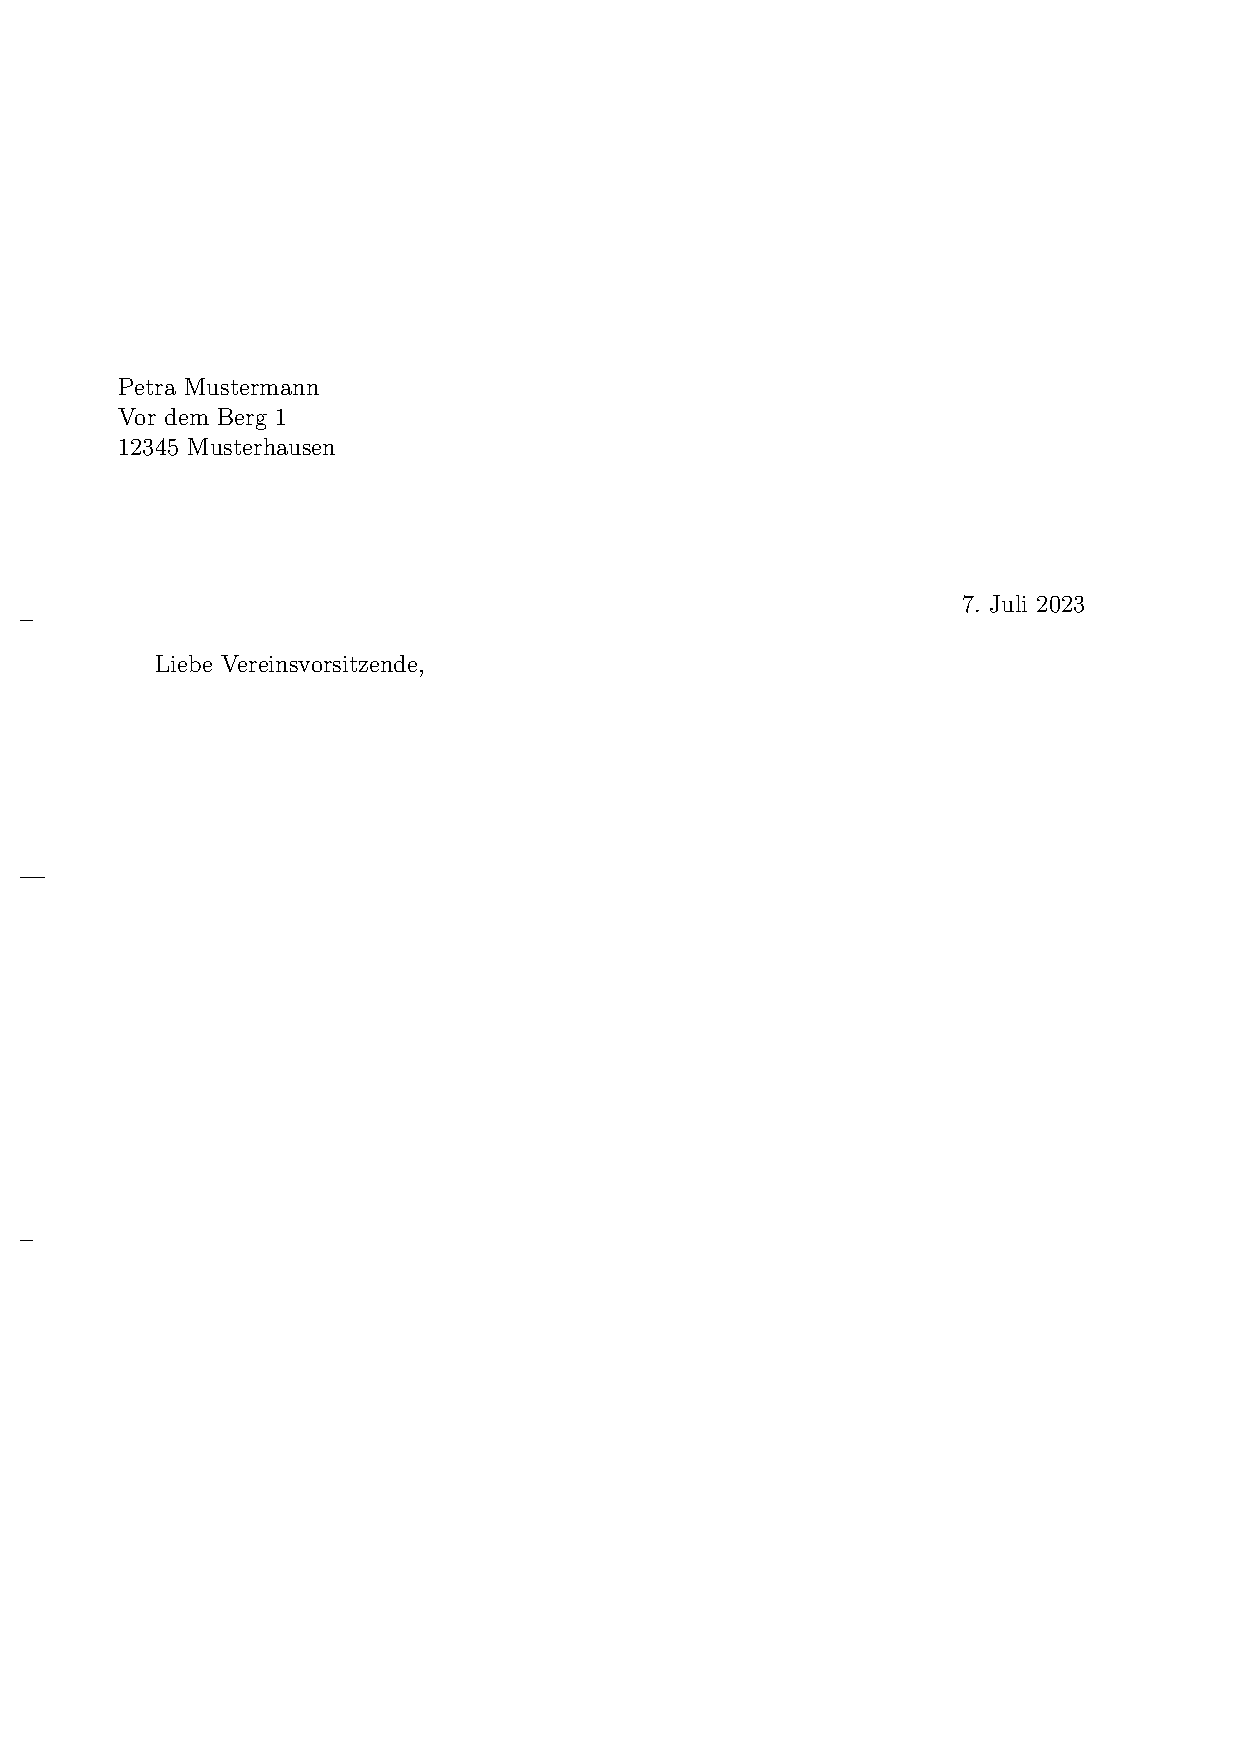
\includegraphics[width=.4\textwidth]{letter-example-00-de}}
    \end{captionbeside}
    \label{fig:\LabelBase.letter-0}
  \end{figure}
\end{Example}
\iffalse % Umbruchkorrekturtext
\begin{Explain}
  Bei\textnote{Tipp!} maschinell erstellten Briefen wurde früher meist auf
  eine Anrede verzichtet, da individualisierte Serienbriefe kaum möglich
  waren. Heute sind persönliche Anreden auch bei Massensendungen üblich.%
\end{Explain}%
\else
\ExampleEndFix% Beispiel am Ende der Beschreibung
\fi
\EndIndexGroup


\begin{Declaration}
  \Macro{closing}\Parameter{Grußfloskel}
\end{Declaration}
Mit der Anweisung \Macro{closing} wird in erster Linie die
\PName{Grußfloskel}\Index{Gruss=Gruß}\Index{Schlussgruss=Schlussgruß}
gesetzt. Diese kann auch mehrzeilig sein. Die einzelnen Zeilen sollten dann
mit doppeltem Backslash voneinander getrennt werden.  Absätze innerhalb der
\PName{Grußfloskel} sind jedoch nicht gestattet.

Darüber hinaus setzt diese Anweisung %
\iffalse% Umbruchkorrekturgelabler
aber auch noch gleich %
\fi%
den Inhalt der Variablen \DescRef{\LabelBase.variable.signature} als
Signatur. Näheres zur Signatur und deren Konfiguration ist
\autoref{sec:\LabelBase.closing} ab
\DescPageRef{\LabelBase.variable.signature} zu entnehmen.

\begin{Example}
  Erweitern wir unser Beispiel um einige Zeilen Brieftext und eine Grußfloskel
  zu:
  \lstinputcode[xleftmargin=1em]{letter-example-01-de.tex}
  Damit sieht das Ergebnis wie in \autoref{fig:\LabelBase.letter-1} aus.
  \begin{figure}
    \setcapindent{0pt}%
    \begin{captionbeside}[{Beispiel: Brief mit Anschrift,
        Anrede, Text und Grußfloskel}]{Ergebnis eines kleinen
        Briefes mit Anschrift, Anrede, Text und Grußfloskel (Datum und
        Faltmarken entstammen den Voreinstellungen für DIN-Briefe)}[l]
      \frame{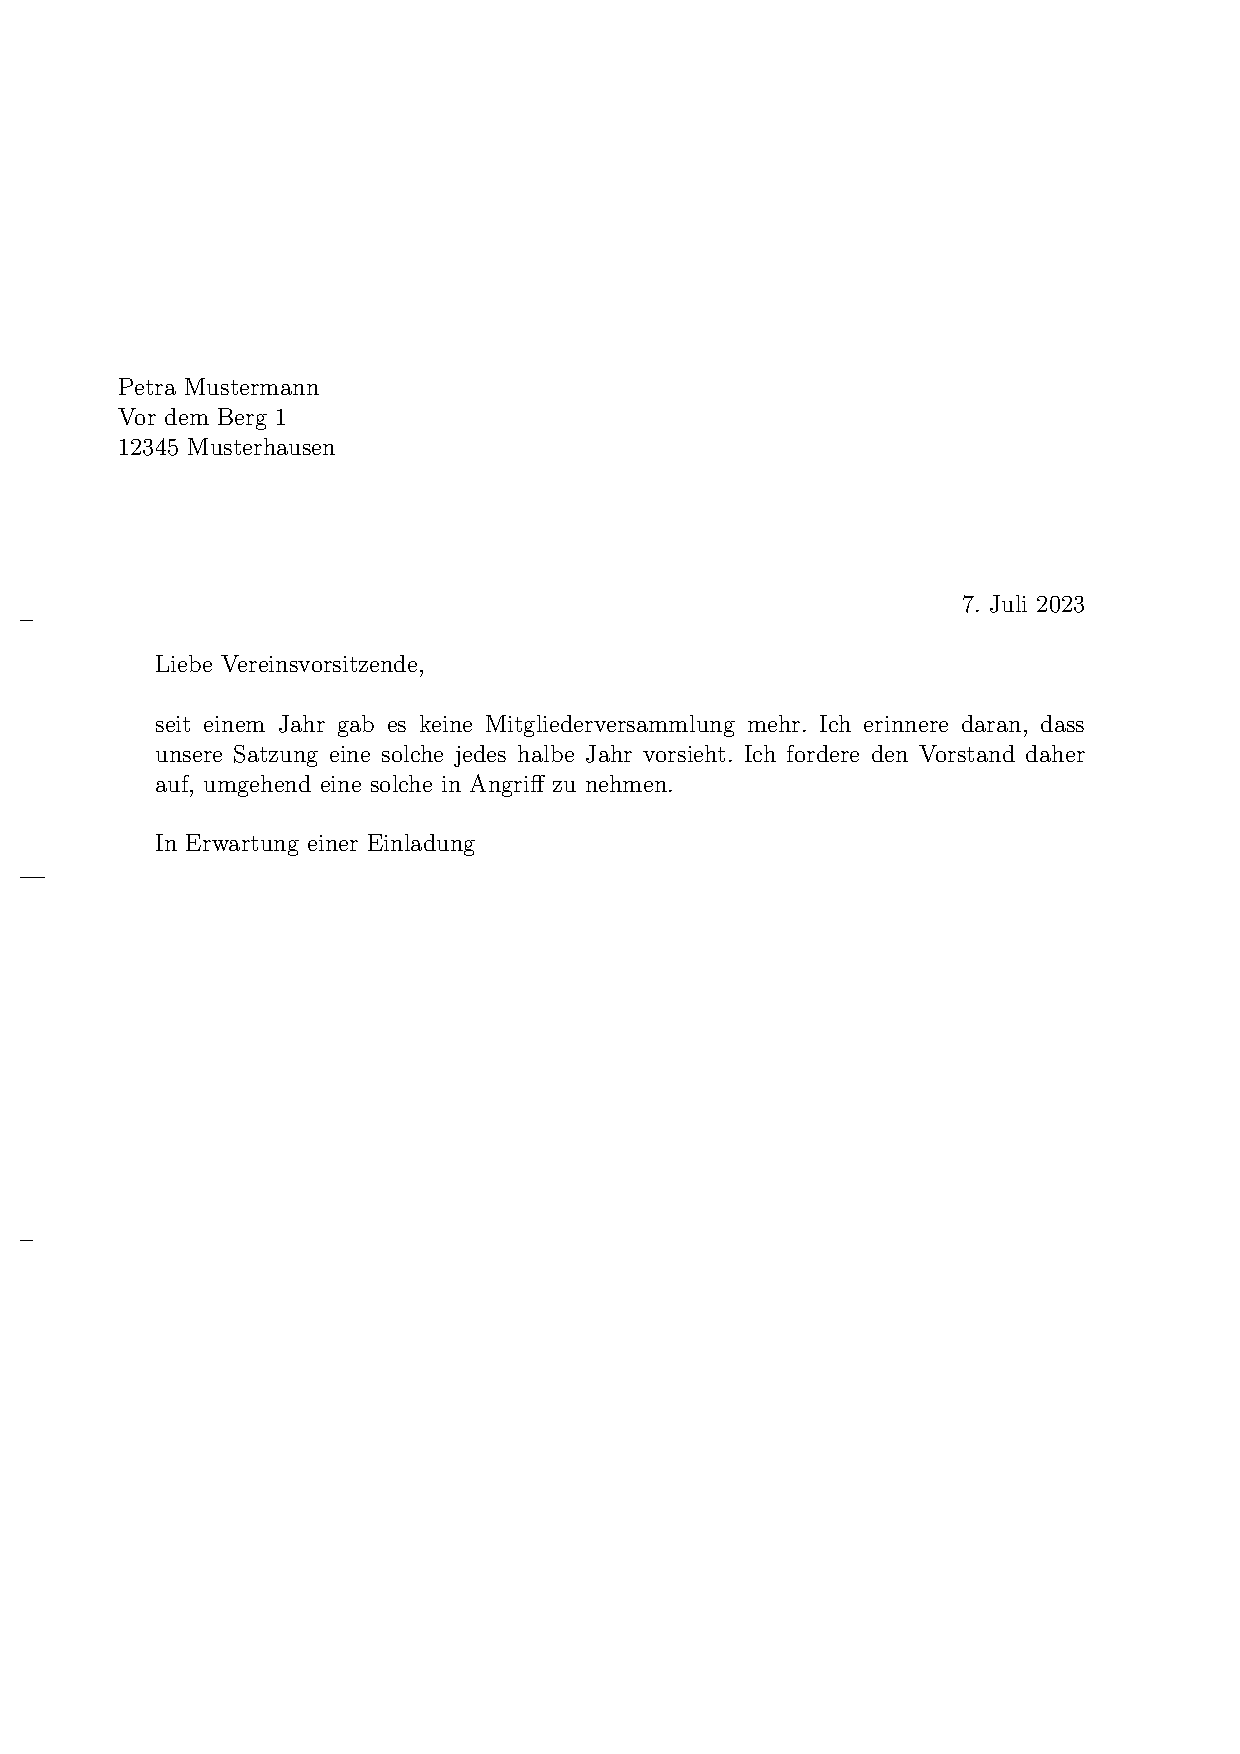
\includegraphics[width=.4\textwidth]{letter-example-01-de}}
    \end{captionbeside}
    \label{fig:\LabelBase.letter-1}
  \end{figure}
\end{Example}
%
\EndIndexGroup
\ExampleEndFix% Beispiel am Ende der Beschreibung


\begin{Declaration}
  \Macro{ps}
\end{Declaration}%
Diese Anweisung schaltet auf das
Postskriptum\Index{Postskriptum} um. Dazu wird ein neuer Absatz
begonnen und ein vertikaler Abstand -- in der Regel zur Signatur --
eingefügt. Auf die Anweisung \Macro{ps} kann beliebiger Text folgen.
Dabei muss der Anwender auch selbst entscheiden, ob er den Nachsatz
etwa mit der Abkürzung »PS:«, die übrigens ohne Punkt gesetzt wird,
beginnen will. \KOMAScript{} setzt diese Abkürzung weder
automatisch noch optional.

\begin{Example}
  Unser Beispielbrief, um ein Postskriptum erweitert,
  \lstinputcode[xleftmargin=1em]{letter-example-02-de.tex}
  sieht dann wie in \autoref{fig:\LabelBase.letter-2} aus.
  \begin{figure}
    \setcapindent{0pt}%
    \begin{captionbeside}[{Beispiel: Brief mit Anschrift,
        Anrede, Text, Grußfloskel und Postskriptum}]{Ergebnis eines kleinen
        Briefes mit Anschrift, Anrede, Text, Grußfloskel und Postskriptum
        (Datum und Faltmarken entstammen den Voreinstellungen für
        DIN-Briefe)}[l]
      \frame{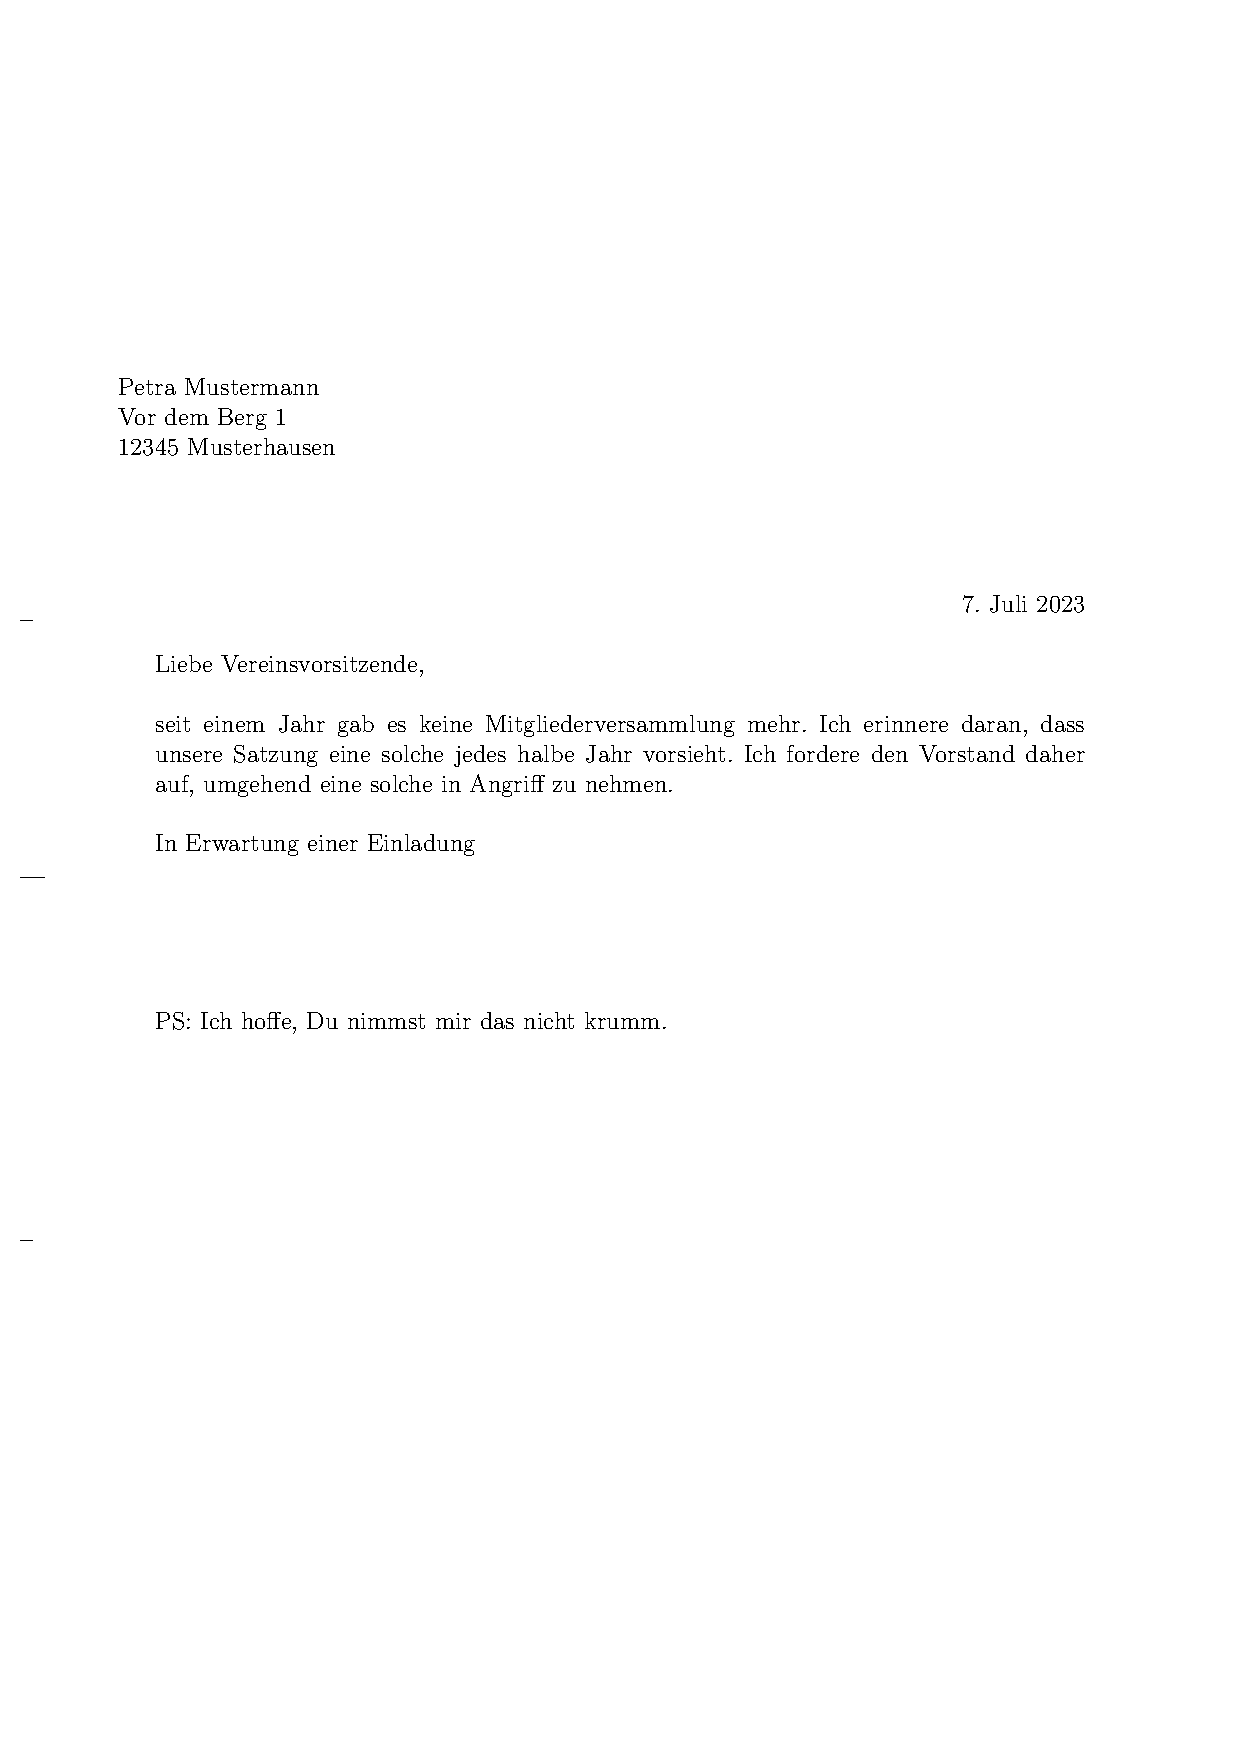
\includegraphics[width=.4\textwidth]{letter-example-02-de}}
    \end{captionbeside}
    \label{fig:\LabelBase.letter-2}
  \end{figure}
\end{Example}%
\iffalse % Umbruchkorrektur
\begin{Explain}%
  Als Briefe noch von Hand geschrieben wurden, war das Postskriptum
  sehr beliebt. Es handelte sich bei diesen Nachsätzen ursprünglich um
  Angaben, die im eigentlichen Brief vergessen wurden. Bei Briefen,
  die mit \LaTeX{} geschrieben werden, ist es natürlich einfach,
  Vergessenes nachträglich in den Brief einzuarbeiten. %
\iftrue % Umbruchkorrektur
  Trotzdem ist das Postskriptum noch immer sehr beliebt, kann man damit doch
  sehr schön noch einmal auf ganz andere äußerst wichtige oder eigentlich
  ganz unwichtige Dinge hinweisen.%
\fi%
\iffalse % Umbruchkorrektur
  Heutzutage verwendet man das Postskriptum dagegen eher für
  Hinweise, die mit dem eigentlichen Briefinhalt wenig zu tun haben.
\fi%
\end{Explain}%
\else%
\ExampleEndFix% Beispiel am Ende
\fi%
%
\EndIndexGroup


\begin{Declaration}
  \Macro{cc}\Parameter{Verteiler}
  \Variable{ccseparator}
\end{Declaration}
Ein \PName{Verteiler}\Index{Verteiler} kann mit der Anweisung \Macro{cc}
gesetzt werden. %
\iftrue% Umbruchkorrektur
Der \PName{Verteiler} wird der Anweisung dabei als Argument übergeben. %
\fi%
Wenn die \PName{Bezeichnung} der Variablen
\Variable{ccseparator}\Index{Trennzeichen} nicht leer ist, wird dem
\PName{Verteiler} die \PName{Bezeichnung} und der \PName{Inhalt} dieser
Variablen vorangestellt. Der \PName{Verteiler} selbst wird dann um die
entsprechende Breite eingerückt ausgegeben. Sollen die einzelnen Einträge
untereinander gesetzt werden, können sie durch doppelten Backslash voneinander
getrennt angegeben werden.
\begin{Example}
  Der Beispielbrief soll dieses Mal nicht nur an die Vorsitzende, sondern mit
  Verteiler auch an alle Mitglieder des Vereins gehen:
  \lstinputcode[xleftmargin=1em]{letter-example-03-de.tex}%
  \iftrue % Umbruchkorrektur (siehe auch unten)
  Das Ergebnis ist in \autoref{fig:\LabelBase.letter-3} zu sehen.%
  \fi%
  \begin{figure}
    \setcapindent{0pt}%
    \begin{captionbeside}[{Beispiel: Brief mit Anschrift,
        Anrede, Text, Grußfloskel, Postskriptum und Verteiler}]{Ergebnis eines
        kleinen Briefes mit Anschrift, Anrede, Text, Grußfloskel, Postskriptum
        und Verteiler (Datum und Faltmarken entstammen den Voreinstellungen
        für DIN-Briefe)}[l]
      \frame{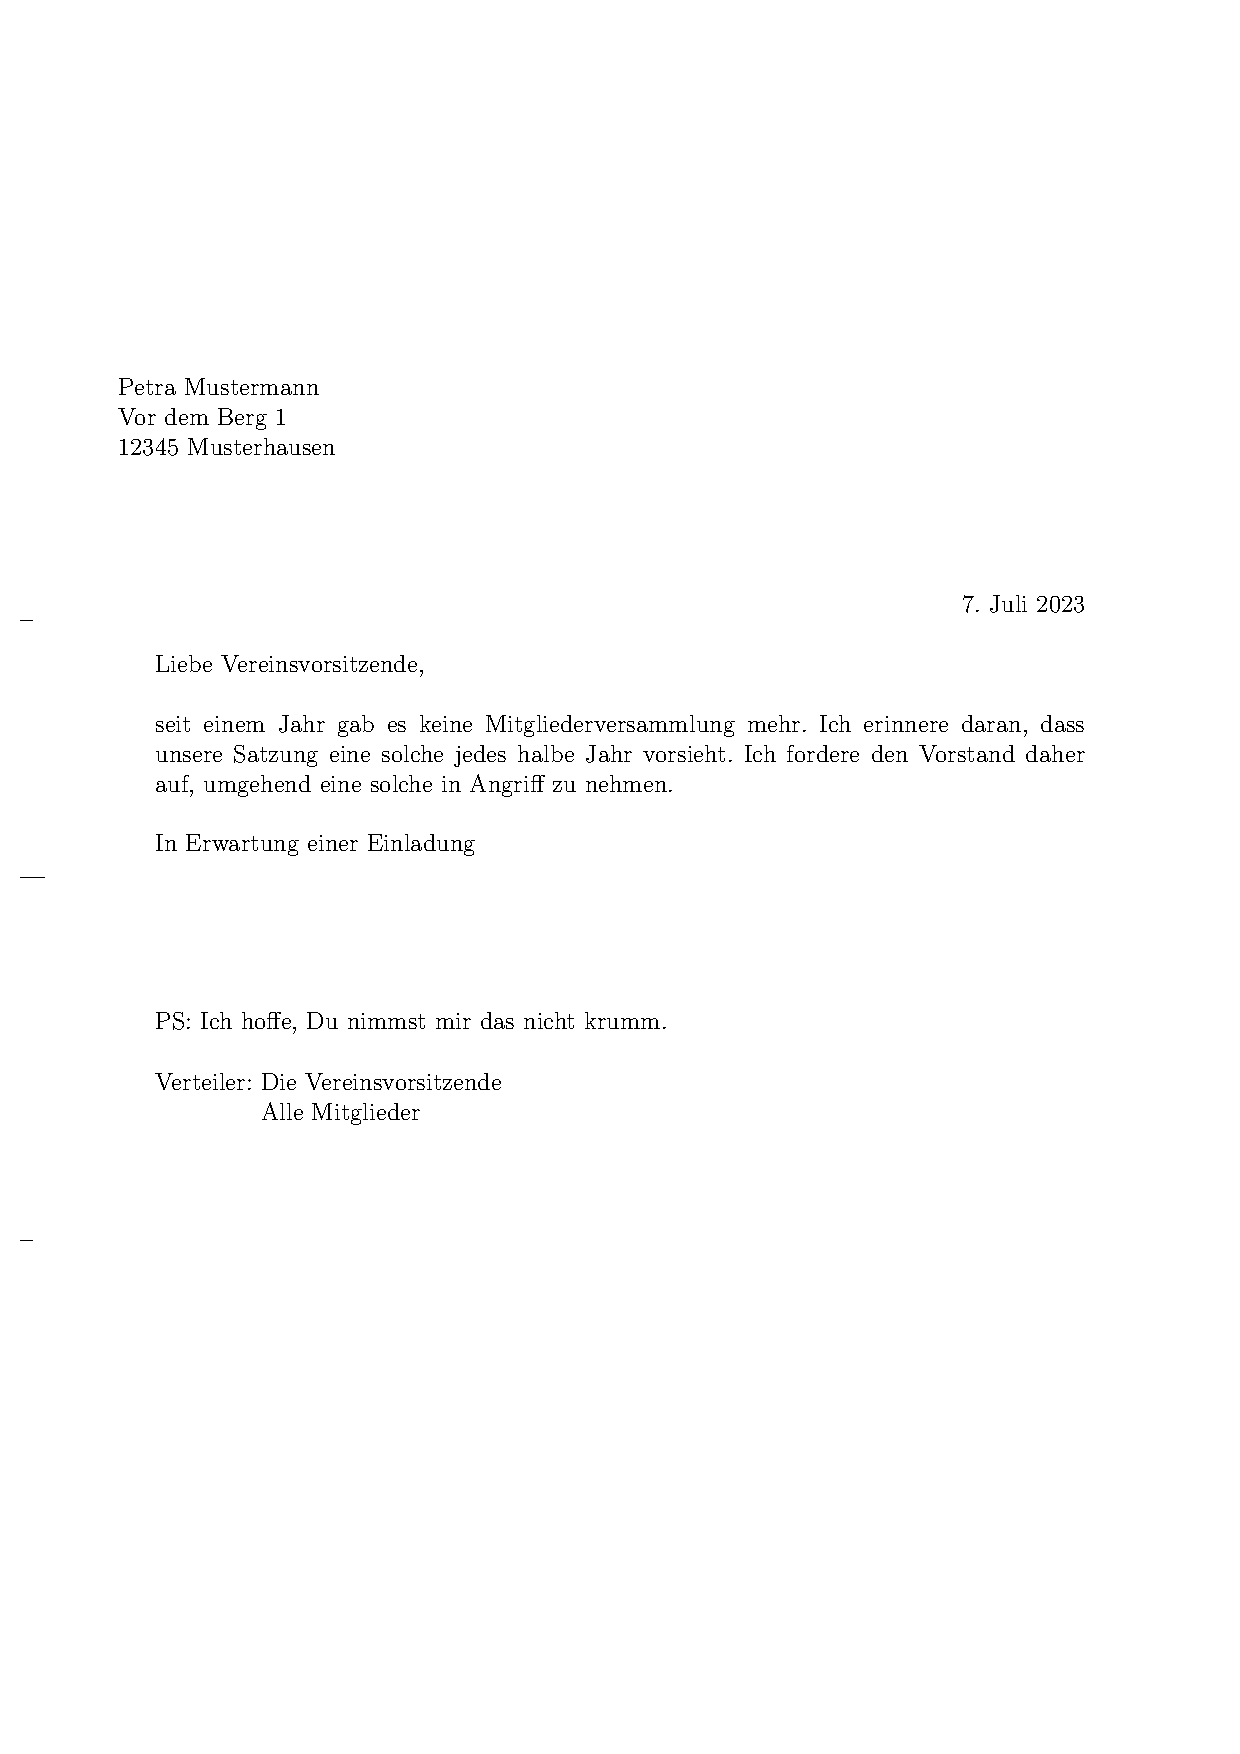
\includegraphics[width=.4\textwidth]{letter-example-03-de}}
    \end{captionbeside}
    \label{fig:\LabelBase.letter-3}
  \end{figure}
\end{Example}
\iftrue% Umbruchkorrektur in Korrelation zu der im Beispiel
Vor dem Verteiler wird automatisch ein Abstand eingefügt.%
\else%
Wie in \autoref{fig:\LabelBase.letter-3} zu sehen, wird vor dem Verteiler
automatisch ein Abstand eingefügt.%
\fi%
%
\EndIndexGroup


\begin{Declaration}
  \Macro{encl}\Parameter{Anlagen}
  \Variable{enclseparator}
\end{Declaration}
Die \PName{Anlagen}\Index{Anlagen} sind genauso aufgebaut wie der
Verteiler. Der einzige Unterschied besteht darin, dass die Einleitung
hier von der \PName{Bezeichnung} und dem \PName{Inhalt} der Variablen
\Variable{enclseparator}\Index{Trennzeichen} bestimmt wird.
\begin{Example}
  Dem Beispielbrief wird nun als Anlage noch ein Auszug aus der Satzung
  beigefügt. Da es nur eine Anlage gibt, wird auch die voreingestellte
  Bezeichnung passend geändert:
  \lstinputcode[xleftmargin=1em]{letter-example-04-de.tex}
  Das Ergebnis ist in \autoref{fig:\LabelBase.letter-4} zu sehen.
  \begin{figure}
    \setcapindent{0pt}%
    \begin{captionbeside}[{Beispiel: Brief mit Anschrift,
        Anrede, Text, Grußfloskel, Postskriptum, Anlagen und
        Verteiler}]{Ergebnis eines kleinen Briefes mit Anschrift, Anrede,
        Text, Grußfloskel, Postskriptum, Anlagen und Verteiler (Datum und
        Faltmarken entstammen den Voreinstellungen für DIN-Briefe)}[l]
      \frame{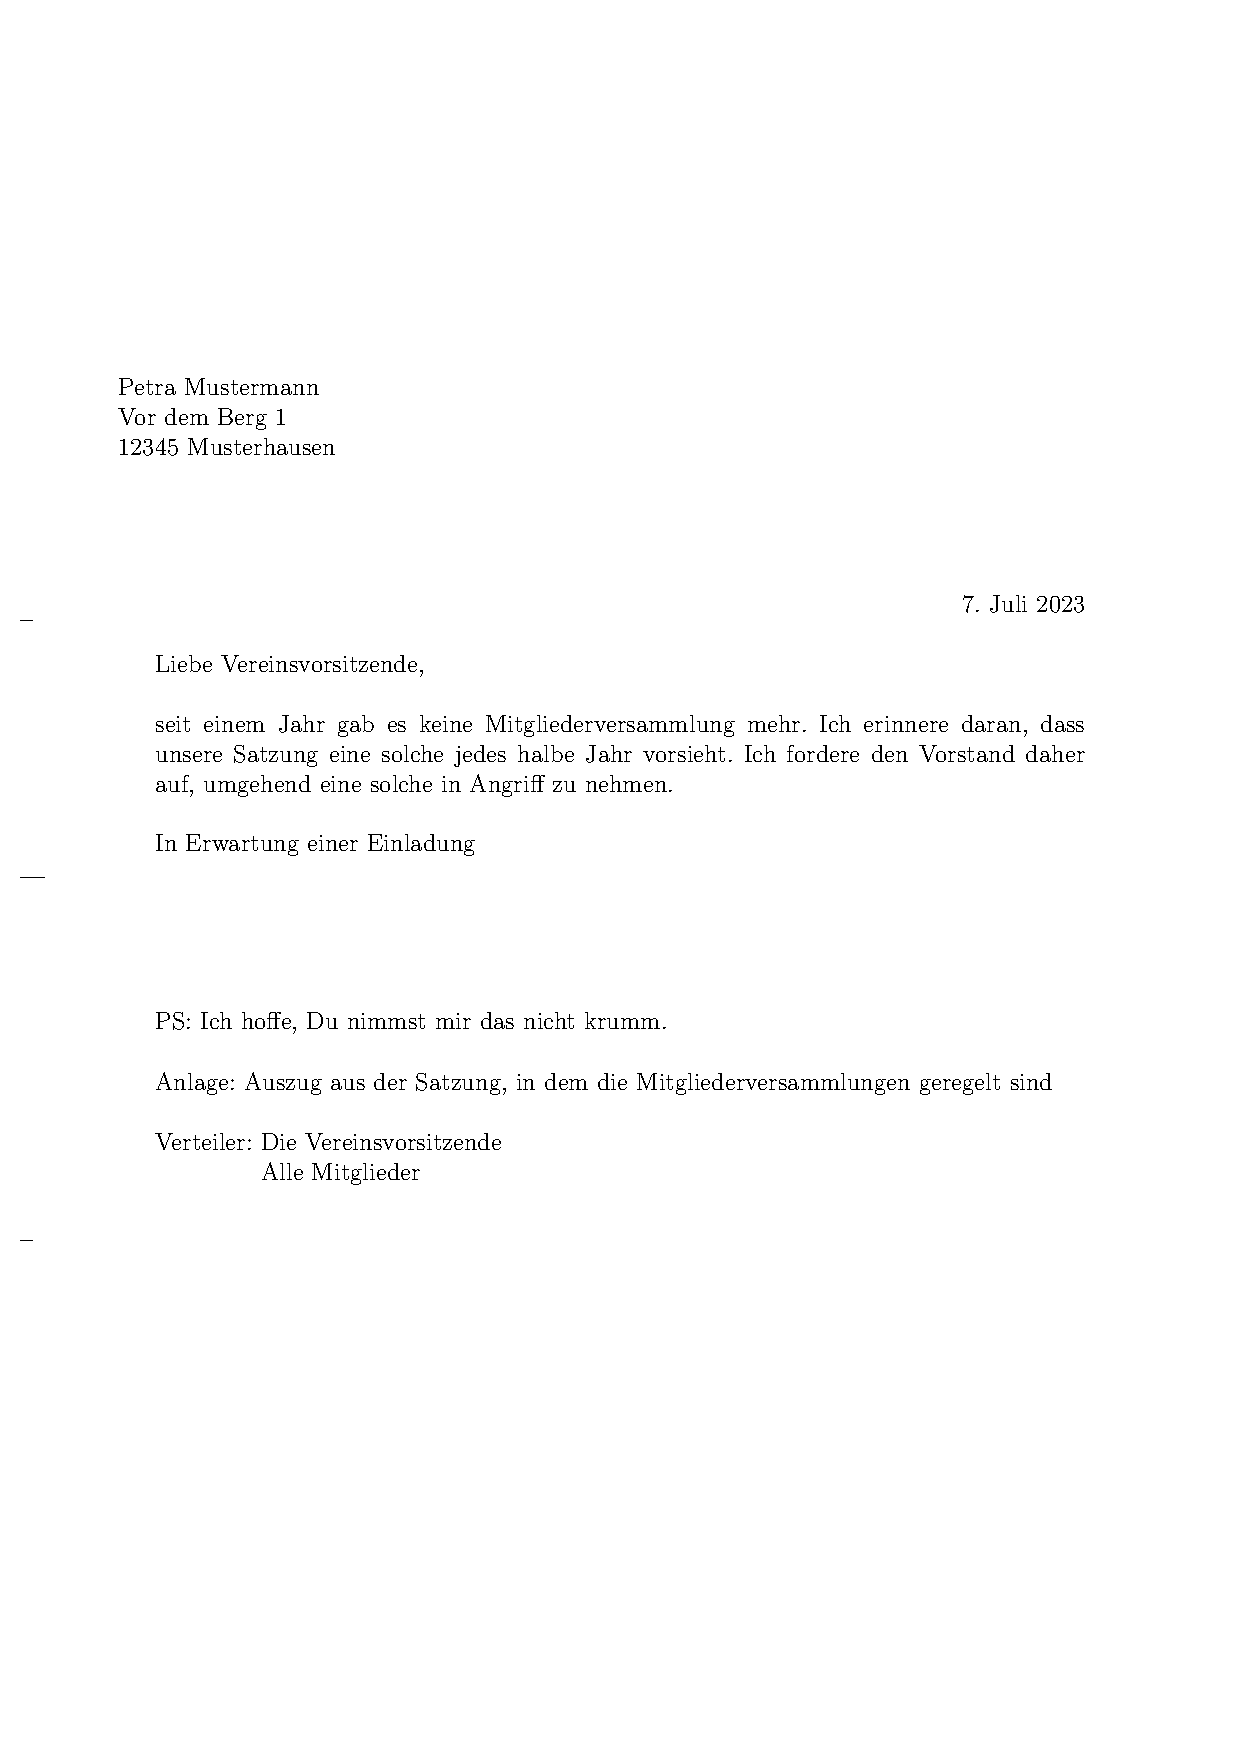
\includegraphics[width=.4\textwidth]{letter-example-04-de}}
    \end{captionbeside}
    \label{fig:\LabelBase.letter-4}
  \end{figure}
\end{Example}
%
\EndIndexGroup
%
\EndIndexGroup

\LoadCommonFile{fontsize} % \section{Wahl der Schriftgröße für das Dokument}

\LoadCommonFile{textmarkup} % \section{Textauszeichnungen}

\section{Briefbogen}
\seclabel{firstpage}
\BeginIndexGroup
\BeginIndex{}{Briefbogen}

Der Briefbogen ist die erste Seite und damit das Aushängeschild jedes
Briefes. Im geschäftlichen Bereich handelt es sich dabei oft um einen
Vordruck, auf dem viele Elemente, wie ein Briefkopf mit Absenderinformationen
und Logo, bereits enthalten sind. Bei \KOMAScript{} sind diese Elemente frei
positionierbar. Damit ist es nicht nur möglich, einen Briefbogen direkt
nachzubilden, sondern auch vorgesehene Felder, wie die Anschrift, unmittelbar
auszufüllen. Die freie Positionierbarkeit wird über Pseudolängen (siehe
\autoref{sec:\LabelBase.pseudoLength} ab
\autopageref{sec:\LabelBase.pseudoLength}) erreicht. Eine schematische
Darstellung des Briefbogens und der dafür verwendeten Variablen ist in
\autoref{fig:\LabelBase.variables} zu finden. Dabei sind die Namen der
Variablen zur besseren Unterscheidung von Anweisungen und deren Argumenten
fett gedruckt.

Folgeseiten\Index{Folgeseite} sind vom Briefbogen zu
unterscheiden. Folgeseiten im Sprachgebrauch dieser Anleitung sind alle
Briefseiten abgesehen von der ersten.


\begin{figure}
  \centering
  \tikzset{x=.56mm,y=-.56mm}
  \tiny
  % ======================================================================
% variables-tikz.tex
% Copyright (c) Markus Kohm, 2005-2022
%
% This file is part of the LaTeX2e KOMA-Script bundle.
%
% This work may be distributed and/or modified under the conditions of
% the LaTeX Project Public License, version 1.3c of the license.
% The latest version of this license is in
%   http://www.latex-project.org/lppl.txt
% and version 1.3c or later is part of all distributions of LaTeX 
% version 2005/12/01 or later and of this work.
%
% This work has the LPPL maintenance status "author-maintained".
%
% The Current Maintainer and author of this work is Markus Kohm.
%
% This work consists of all files listed in MANIFEST.md.
% ======================================================================
%
% Generation of plength figures at scrlttr2 chapter of the KOMA-Script
% guide
%
% Maintained by Markus Kohm
% Original metapost source by Stephan Hennig
% Original TikZ source by Marei Peischl
%
% ======================================================================

\KOMAProvidesFile{variables-tikz.tex}%
                 [$Date: 2022-06-05 12:40:11 +0200 (So, 05. Jun 2022) $
                  KOMA-Script guide (figure in scrlttr2.tex)]
                 
\ExplSyntaxOn
\prop_if_exist:NF \l_this_plength_description_prop {
  \prop_new:N \l_this_plength_description_prop
}
\prop_set_from_keyval:Nn \l_this_plength_description_prop {
  firsthead=\Multi{\DescRef{scrlttr2.variable.firsthead}\\
    \DescRef{scrlttr2.variable.fromname}\and
    \DescRef{scrlttr2.variable.fromaddress}\and
    \DescRef{scrlttr2.variable.fromphone}\and
    \DescRef{scrlttr2.variable.fromfax}\and
    \DescRef{scrlttr2.variable.fromemail}\and
    \DescRef{scrlttr2.variable.fromurl}},
  firstfoot=\DescRef{scrlttr2.variable.firstfoot},
  backaddress =\DescRef{scrlttr2.variable.backaddress},
  specialmail=\DescRef{scrlttr2.variable.specialmail},
  refline=\Multi{\DescRef{scrlttr2.variable.yourref}\and
    \DescRef{scrlttr2.variable.yourmail}\and
    \DescRef{scrlttr2.variable.myref}\and
    \DescRef{scrlttr2.variable.customer}\and
    \DescRef{scrlttr2.variable.invoice}\and
    \DescRef{scrlttr2.variable.place}\and
    \DescRef{scrlttr2.variable.date}},
  title=\DescRef{scrlttr2.variable.title},
  subject=\DescRef{scrlttr2.variable.subject},
  signature=\DescRef{scrlttr2.variable.signature},
  location= \DescRef{scrlttr2.variable.location},
  toaddr=\Macro{begin}\PParameter{\DescRef{scrlttr2.env.letter}}\Parameter{\toaddrname},
  opening=\DescRef{scrlttr2.cmd.opening}\Parameter{\openingargumentname},
  body=\desc\letterbodyname,
  closing=\DescRef{scrlttr2.cmd.closing}\Parameter{\closingargumentname},
}

\prop_if_exist:NF \l_this_plength_var_prop {
  \prop_new:N \l_this_plength_var_prop
}

\prop_set_from_keyval:Nn \l_this_plength_var_prop {
  ticksize=1,
  textwidth= 147,
  textheight= 209.4,
  evensidemargin= 6.1,
  oddsidemargin = 6.1,
  paperwidth = 210,
  paperheight = 297,
  baselineskip = .9\baselineskip, %3.86607,
  headheight     =  6,
  headsep        =7.2,
  footskip       =16.73,
  foldmarkhpos = 3.5,
  tfoldmarkvpos = 105,
  bfoldmarkvpos = 210,
  tfoldmarklength = 2,
  pfoldmarklength = 4,
  bfoldmarklength = 2,
  toaddrvpos = 45,
  refvpos = 98.5,
  refaftervskip = \UseVar{baselineskip},
  toaddrhpos = 20,
  toaddrwidth = 85,
  toaddrheight = 40,
  toaddrindent = 6,
  specialmailwidth = 50,
  specialmailrightindent = 4,
  specialmailheight = \UseVar{baselineskip},
  locwidth = 37.5,
  backaddrheight = 5,
  firstheadvpos = 8,
  firstheadwidth = \UseVar{paperwidth} - 2 * \UseVar{toaddrhpos},
  firstfootwidth = \UseVar{firstheadwidth},
  firstfootvpos =  16.58 + \UseVar{headheight} + \UseVar{headsep} + \UseVar{textheight} + \UseVar{footskip},
  refwidth = 0,
  sigindent = 0,
  toaddrindent =0,
  sigbeforevskip = 2*\UseVar{baselineskip},
  firstheadhpos = 0.5* \UseVar{paperwidth}-.5*\UseVar{firstheadwidth},
  firstheadheight = 5*\UseVar{baselineskip},
  firstfoothpos = 0.5*(\UseVar{paperwidth}-\UseVar{firstfootwidth}),
  firstfootheight = 3*\UseVar{baselineskip},
  fromrulewidth = 0.5 * \UseVar{firstheadwidth},
  lochpos = \UseVar{paperwidth}-\UseVar{toaddrhpos}-\UseVar{locwidth},
  refhpos = 25.40+\UseVar{oddsidemargin},
  text = \UseVar{refhpos},
  textcenter = \UseVar{refhpos}+0.5*\UseVar{textwidth},
  refheight = 2*\UseVar{baselineskip},
  refwidth = \UseVar{textwidth},
  titlevpos = \UseVar{refvpos}+\UseVar{refheight}+\UseVar{refaftervskip},
  titlewidth = 90,
  titleheight = 1.2*\UseVar{baselineskip},
  subjectvpos = \UseVar{titlevpos}+\UseVar{titleheight}+1*\UseVar{baselineskip},
  subjectwidth = 80,
  subjectheight = \UseVar{baselineskip},
  openingvpos = \UseVar{subjectvpos}+\UseVar{subjectheight}+2*\UseVar{baselineskip},
  openingwidth = 60,
  openingheight = \UseVar{baselineskip},
  bodyvpos = \UseVar{openingvpos}+\UseVar{openingheight}+\UseVar{baselineskip},
  bodywidth = \UseVar{textwidth},
  bodyheight = 6*\UseVar{baselineskip},
  typeareabottom = \UseVar{firstfootvpos}-\UseVar{footskip},
  sigvpos = \UseVar{bodyvpos}+\UseVar{bodyheight}+\UseVar{baselineskip},
  sigwidth = 50,
  sigheight = \UseVar{baselineskip},
  locvpos = \UseVar{toaddrvpos},
  locheight = \UseVar{toaddrheight},
}
\def\UseVar#1{
  \fp_eval:n {\prop_item:Nn \l_this_plength_var_prop {#1}}
}

\def\UseDesc#1{
  \prop_item:Nn \l_this_plength_description_prop {#1}
}

\ExplSyntaxOff

\def\desc{\itshape}

\providecommand*{\Multi}[1]{%
  {\def\and{, }%
    \begin{tabular}{@{}l@{}}
      #1
    \end{tabular}
  }%
}

\begin{tikzpicture}[fill=black!20]
  \draw (0,0)rectangle (\UseVar{paperwidth},\UseVar{paperheight});
  
  \filldraw(\UseVar{firstheadhpos},\UseVar{firstheadvpos})rectangle node{\UseDesc{firsthead}}+(\UseVar{firstheadwidth},\UseVar{firstheadheight});
  
  \filldraw(\UseVar{toaddrhpos},\UseVar{toaddrvpos}) rectangle
  node {\UseDesc{backaddress}}
  +(\UseVar{toaddrwidth},\UseVar{backaddrheight});
  
  \filldraw(\UseVar{toaddrhpos}+.5*\UseVar{toaddrwidth}-\UseVar{specialmailrightindent},\UseVar{toaddrvpos}+\UseVar{backaddrheight}) rectangle
  node {\UseDesc{specialmail}}
  +(.5*\UseVar{toaddrwidth},\UseVar{specialmailheight});
  
  \filldraw(\UseVar{toaddrhpos}+\UseVar{toaddrindent},\UseVar{toaddrvpos}+\UseVar{backaddrheight}+\UseVar{specialmailheight})
  rectangle node {\UseDesc{toaddr}}
  +(\UseVar{toaddrwidth}-2*\UseVar{toaddrindent},\UseVar{toaddrheight}-\UseVar{backaddrheight}-\UseVar{specialmailheight});
  
  \draw(\UseVar{toaddrhpos},\UseVar{toaddrvpos})rectangle+(\UseVar{toaddrwidth},\UseVar{toaddrheight});
  
  \filldraw (\UseVar{refhpos},\UseVar{refvpos})rectangle node{\UseDesc{refline}}
  +(\UseVar{refwidth},\UseVar{refheight});
  
  \filldraw (\UseVar{textcenter}-.5*\UseVar{titlewidth},\UseVar{titlevpos})rectangle node{\UseDesc{title}}
  +(\UseVar{titlewidth},\UseVar{titleheight});
  
  \filldraw (\UseVar{text},\UseVar{subjectvpos})rectangle node{\UseDesc{subject}}
  +(\UseVar{subjectwidth},\UseVar{subjectheight});
  
  \filldraw (\UseVar{text},\UseVar{openingvpos})rectangle node{\UseDesc{opening}}
  +(\UseVar{openingwidth},\UseVar{openingheight});
  
  \filldraw (\UseVar{text},\UseVar{bodyvpos})rectangle node{\UseDesc{body}}
  +(\UseVar{bodywidth},\UseVar{bodyheight});
  
  \filldraw (\UseVar{text}+\UseVar{sigindent},\UseVar{sigvpos})rectangle node{\UseDesc{closing}}
  +(\UseVar{sigwidth},\UseVar{sigheight});
  
  \filldraw (\UseVar{text}+\UseVar{sigindent}+.1*\UseVar{sigwidth},\UseVar{sigvpos}+\UseVar{sigheight}+\UseVar{sigbeforevskip})rectangle node{\UseDesc{signature}}
  +(.8*\UseVar{sigwidth},\UseVar{sigheight});
  
  \filldraw (\UseVar{lochpos},\UseVar{locvpos}) rectangle node{\UseDesc{location}}+(\UseVar{locwidth},\UseVar{locheight});
  
  \filldraw (\UseVar{firstfoothpos},\UseVar{firstfootvpos}) rectangle node{\UseDesc{firstfoot}} +(\UseVar{firstfootwidth},\UseVar{firstfootheight});
  
  \draw[thick] (\UseVar{foldmarkhpos},\UseVar{tfoldmarkvpos}) --+(\UseVar{tfoldmarklength},0);
  \draw[thick] (\UseVar{foldmarkhpos},.5*\UseVar{paperheight}) --+(\UseVar{pfoldmarklength},0);
  \draw[thick] (\UseVar{foldmarkhpos},\UseVar{bfoldmarkvpos}) --+(\UseVar{bfoldmarklength},0);
\end{tikzpicture}

\endinput

%%% Local Variables: 
%%% mode: latex
%%% coding: utf-8
%%% End: 

  \caption{Schematische Darstellung des Briefbogens mit den wichtigsten
    Anweisungen und Variablen für die skizzierten Elemente}
  \label{fig:\LabelBase.variables}
\end{figure}


\subsection{Faltmarken}
\seclabel{foldmarks}
\BeginIndexGroup
\BeginIndex{}{Faltmarke}%

Falt- oder Falzmarken sind kleine horizontale Striche am linken und kleine
vertikale Striche am oberen Rand. \KOMAScript{} unterstützt für den Briefbogen
derzeit drei konfigurierbare horizontale und eine konfigurierbare vertikale
Faltmarke. Dazu wird noch eine horizontale Loch- oder Seitenmittenmarke
unterstützt, die nicht in der Vertikalen verschoben werden kann.

\begin{Declaration}
  \OptionVName{foldmarks}{Einstellung}
\end{Declaration}
Mit der Option \Option{foldmarks} können Faltmarken\Index{Faltmarke} für eine
vertikale Zwei"~, Drei- oder Vierteilung und eine horizontale Zweiteilung
aktiviert oder deaktiviert werden. Die einzelnen Teile müssen dabei nicht
äquidistant sein. Die Positionen von drei der vier horizontalen und der
vertikalen Marke sind über Pseudolängen konfigurierbar (siehe
\autoref{sec:\LabelBase.pseudoLength},
\autopageref{sec:\LabelBase.pseudoLength}).

Über die Option \Option{foldmarks} können entweder mit den Standardwerten für
einfache Schalter, die in \autoref{tab:truefalseswitch},
\autopageref{tab:truefalseswitch} angegeben sind, alle konfigurierten
Faltmarken am linken und oberen Rand ein- und ausgeschaltet werden,
oder\ChangedAt{v2.97e}{\Class{scrlttr2}} es kann durch die Angabe eines oder
mehrerer Buchstaben aus \autoref{tab:\LabelBase.foldmark} die Verwendung der
einzelnen Faltmarken gezielt konfiguriert werden. Auch in diesem Fall werden
die Faltmarken nur dann angezeigt, wenn die Faltmarken nicht mit
\PValue{false}, \PValue{off} oder \PValue{no} generell abgeschaltet
wurden. Die genaue Position der Faltmarken ist von den Einstellungen des
Anwenders beziehungsweise der \File{lco}-Dateien (siehe
\autoref{sec:\LabelBase.lcoFile} ab \autopageref{sec:\LabelBase.lcoFile})
abhängig. Voreingestellt sind \PValue{true} und
\PValue{TBMPL}.\textnote{Voreinstellung}
%
\begin{table}
%  \centering
  \KOMAoptions{captions=topbeside}%
  \setcapindent{0pt}%
%  \caption
  \begin{captionbeside}[{%
      Kombinierbare Werte für die Konfiguration der Faltmarken mit der
      Option \Option{foldmarks}%
    }]{%
      \hspace{0pt plus 1ex}%
      Kombinierbare Werte für die Konfiguration der Faltmarken mit der
      Option \Option{foldmarks}\label{tab:\LabelBase.foldmark}%
    }[l]
  \begin{tabular}[t]{ll}
    \toprule
    \PValue{B} & untere, horizontale Faltmarke am linken Rand aktivieren\\%
    \PValue{b} & untere, horizontale Faltmarke am linken Rand deaktivieren\\%
    \PValue{H} & alle horizontalen Faltmarken am linken Rand aktivieren\\%
    \PValue{h} & alle horizontalen Faltmarken am linken Rand deaktivieren\\%
    \PValue{L} & linke, vertikale Faltmarke am oberen Rand aktivieren\\%
    \PValue{l} & linke, vertikale Faltmarke am oberen Rand deaktivieren\\%
    \PValue{M} & mittlere, horizontale Faltmarke am linken Rand aktivieren\\%
    \PValue{m} & mittlere, horizontale Faltmarke am linken Rand deaktivieren\\%
    \PValue{P} & Locher- bzw. Seitenmittenmarke am linken Rand aktivieren\\%
    \PValue{p} & Locher- bzw. Seitenmittenmarke am linken Rand deaktivieren\\%
    \PValue{T} & obere, horizontale Faltmarke am linken Rand aktivieren\\%
    \PValue{t} & obere, horizontale Faltmarke am linken Rand deaktivieren\\%
    \PValue{V} & alle vertikalen Faltmarken am oberen Rand aktivieren\\%
    \PValue{v} & alle vertikalen Faltmarken am oberen Rand deaktivieren\\
    \bottomrule
  \end{tabular}
  \end{captionbeside}
\end{table}
\begin{Example}
  Angenommen, Sie wollen alle Faltmarken außer der Lochermarke
  abschalten. Wenn die Voreinstellung zuvor noch nicht geändert wurde, können
  Sie das Abschalten wie folgt erreichen:
\begin{lstcode}
  \KOMAoptions{foldmarks=blmt}
\end{lstcode}
  Besteht die Möglichkeit, dass die Voreinstellung bereits geändert wurde, so
  sollten Sie lieber auf Nummer Sicher gehen. Unser Beispiel ist dann
  entsprechend abzuändern.%
  \lstinputcode[xleftmargin=1em]{letter-example-07-de.tex}%
  Das Ergebnis ist in \autoref{fig:\LabelBase.letter-7} zu sehen.
  \begin{figure}
    \setcapindent{0pt}%
    \begin{captionbeside}[{Beispiel: Brief mit Anschrift,
        Anrede, Text, Grußfloskel, Postskriptum, Anlagen, Verteiler und
        Lochermarke}]{Ergebnis eines kleinen Briefes mit Anschrift, Anrede,
        Text, Grußfloskel, Postskriptum, Anlagen, Verteiler und Lochermarke
        (das Datum entstammt den Voreinstellungen für DIN-Briefe)}[l]
      \frame{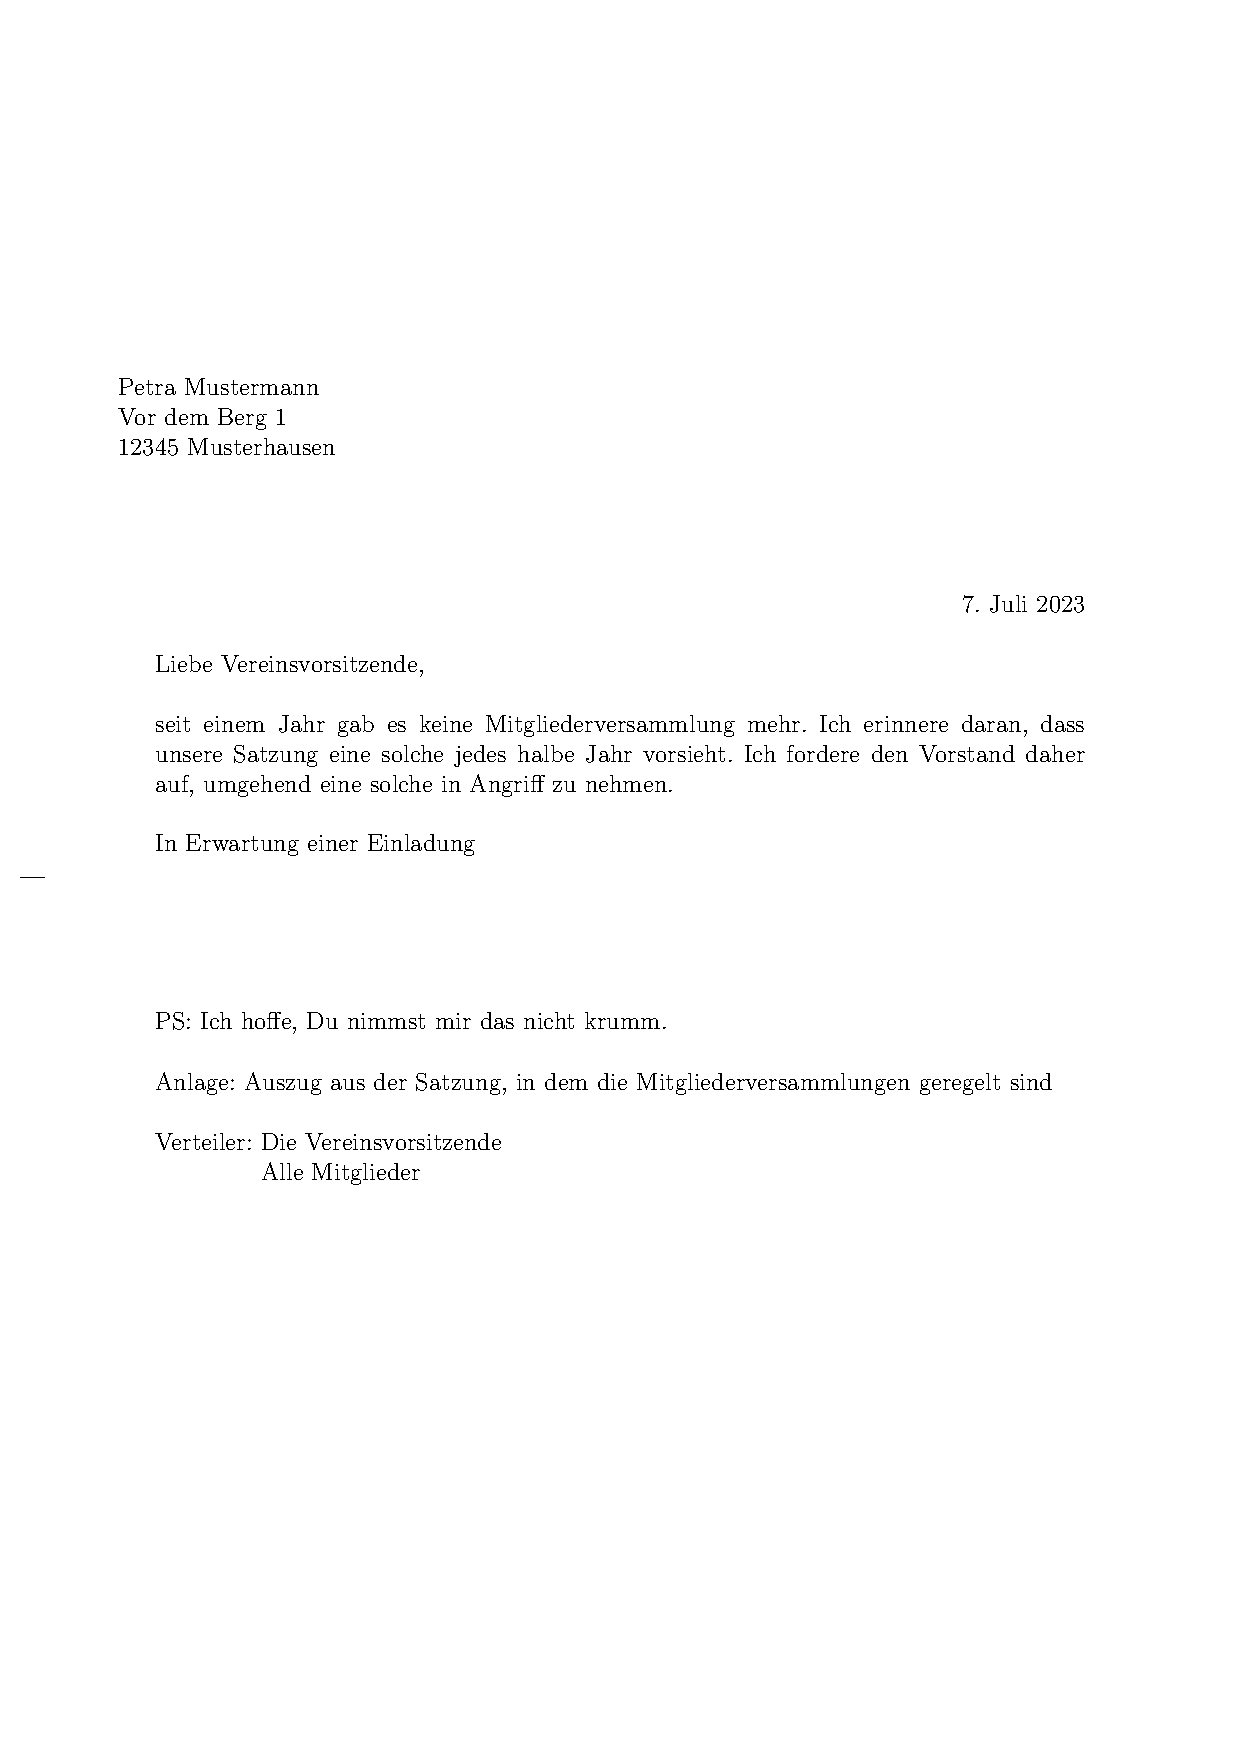
\includegraphics[width=.4\textwidth]{letter-example-07-de}}
    \end{captionbeside}
    \label{fig:\LabelBase.letter-7}
  \end{figure}
\end{Example}
\BeginIndex{FontElement}{foldmark}\LabelFontElement{foldmark}%
Über\ChangedAt{v2.97c}{\Class{scrlttr2}} das Element \FontElement{foldmark}
kann die Farbe der Faltmarken geändert werden. Dazu werden die Anweisungen
\DescRef{\LabelBase.cmd.setkomafont} und
\DescRef{\LabelBase.cmd.addtokomafont} (siehe
\autoref{sec:\LabelBase.textmarkup}, \DescPageRef{\LabelBase.cmd.setkomafont})
verwendet. Voreingestellt ist keine Änderung.%
\EndIndexGroup


\begin{Declaration}
  \PLength{tfoldmarkvpos}
  \PLength{mfoldmarkvpos}
  \PLength{bfoldmarkvpos}
\end{Declaration}
\KOMAScript{} kennt für Briefe \Class{scrlttr2} insgesamt drei in der vertikalen
Platzierung konfigurierbare Faltmarken. Die Position der oberen Faltmarke vom
oberen Papierrand wird von der Pseudolänge \PLength{tfoldmarkvpos}
bestimmt. Für die Position der mittleren Faltmarke ist Pseudolänge
\PLength{mfoldmarkvpos}\ChangedAt{v2.97e}{\Class{scrlttr2}}, für die untere
Faltmarke \PLength{bfoldmarkvpos} zuständig. Mit der
Locher-\Index{Lochermarke} oder Seitenmittenmarke kommt noch eine weitere
horizontale Marke dazu. Diese wird jedoch immer in der vertikalen Seitenmitte
platziert. 
\iffalse% Umbruchkorrekturtext!
Da ihre vertikale Position also nicht konfigurierbar ist, existiert
auch keine Pseudolänge dafür.
\fi

Die\important{Achtung!} obere und untere Faltmarke dienen nicht der exakten
Drittelung des Papiers beim Falten. Vielmehr soll das Papier mit ihrer Hilfe
so geknickt werden können, dass das Feld für die Anschrift in einem
Fensterbriefumschlag zu sehen ist. Die Einstellungen sind daher von den
\File{lco}-Dateien\textnote{\File{lco}-Datei}%
\Index{lco-Datei=\File{lco}-Datei} abhängig. Eine
Besonderheit\textnote{Achtung!} stellt \Option{DINmtext} dar. Hier wird
von einem Briefumschlag im Format C6/5 (auch »C6 lang« genannt)
ausgegangen. Briefe, die mit dieser Option erstellt wurden, sind normalerweise
nicht für Fensterbriefumschläge im Format C5 oder C4 geeignet.

Die mittlere Faltmarke wird für abendländische Briefe normalerweise nicht
benötigt. Beispielsweise in Japan gibt es jedoch so unterschiedliche
Briefumschläge, dass eine weitere Faltmarke benötigt wurde (siehe die
japanischen \File{lco}-Dateien). An dieser Stelle sei darauf hingewiesen, dass
die Bezeichnungen »obere«, »mittlere« und »untere« Faltmarke lediglich eine
Sprachkonvention darstellen. Tatsächlich ist nicht festgelegt, dass
\PLength{tfoldmarkvpos} kleiner als \PLength{mfoldmarkvpos} und dieses kleiner
als \PLength{bfoldmarkvpos} sein muss. Ist\textnote{Achtung!} eine der
Pseudolängen hingegen Null, so wird die entsprechende Faltmarke auch dann
nicht gesetzt, wenn sie per Option \DescRef{\LabelBase.option.foldmarks}%
\IndexOption{foldmarks~=\PName{Einstellung}}%
\important{\DescRef{\LabelBase.option.foldmarks}} (siehe
\DescPageRef{\LabelBase.option.foldmarks}) explizit aktiviert wurde.%
\EndIndexGroup


\begin{Declaration}
  \PLength{tfoldmarklength}
  \PLength{mfoldmarklength}
  \PLength{bfoldmarklength}
  \PLength{pfoldmarklength}
\end{Declaration}
Diese\ChangedAt{v2.97e}{\Class{scrlttr2}} vier Pseudolängen bestimmen die
Länge der vier horizontalen Marken. Dabei gilt eine
Besonderheit. Ist\textnote{Achtung!} die Länge nämlich mit Null angegeben, so
werden bei den Pseudolängen \PLength{tfoldmarklength},
\PLength{mfoldmarklength} und \PLength{bfoldmarklength} für die drei in der
vertikalen Position konfigurierbaren Faltmarken stattdessen 2\Unit{mm} als
Länge verwendet. Die Länge der Lochermarke, \PLength{pfoldmarklength}, wird
hingegen auf 4\Unit{mm} gesetzt.%
\EndIndexGroup


\begin{Declaration}
  \PLength{foldmarkhpos}
\end{Declaration}
Diese Pseudolänge gibt den Abstand aller horizontalen Faltmarken vom linken
Papier\-rand an.  Normalerweise sind das 3{,}5\Unit{mm}. Sie\textnote{Tipp!}
können den Wert aber auch in Ihrer eigenen \File{lco}-Datei ändern, falls Sie
einen Drucker verwenden, der einen breiteren unbedruckbaren linken Rand
hat. Ob die Faltmarken überhaupt gesetzt werden, hängt außerdem von der Option
\DescRef{\LabelBase.option.foldmarks}%
\important{\DescRef{\LabelBase.option.foldmarks}}%
\IndexOption{foldmarks~=\PName{Einstellung}} ab (siehe
\DescPageRef{\LabelBase.option.foldmarks}).%
%
\EndIndexGroup


\begin{Declaration}
  \PLength{lfoldmarkhpos}
\end{Declaration}
Neben\ChangedAt{v2.97e}{\Class{scrlttr2}} den horizontalen Faltmarken gibt es
auch noch eine vertikale Faltmarke. Deren Abstand von der linken Papierkante
wird über die Pseudolänge \PLength{lfoldmarkhpos} bestimmt. Diese Faltmarke
wird beispielsweise bei Briefen für einige japanische Chou- oder You-Umschläge
benötigt, wenn man diese für A4-Papier verwenden
will. In\textnote{Voreinstellung} den japanischen
\File{lco}-Dateien\Index{lco-Datei=\File{lco}-Datei} (siehe
\autoref{sec:\LabelBase.lcoFile} ab \autopageref{sec:\LabelBase.lcoFile}) ist
daher ein Wert von 202\Unit{mm} voreingestellt. Mit der Voreinstellung Null
der übrigen \File{lco}-Dateien wird auch dann keine Marke ausgegeben, wenn sie
per Option \DescRef{\LabelBase.option.foldmarks}%
\important{\DescRef{\LabelBase.option.foldmarks}}%
\IndexOption{foldmarks~=\PName{Einstellung}} (siehe
\DescPageRef{\LabelBase.option.foldmarks}) aktiviert wird.%
\EndIndexGroup


\begin{Declaration}
  \PLength{lfoldmarklength}
\end{Declaration}
Die Pseudolänge \PLength{lfoldmarklength} bestimmt
die\ChangedAt{v2.97e}{\Class{scrlttr2}} Länge der vertikalen
Faltmarke. Auch\textnote{Achtung!}  hier gibt es die Besonderheit, dass bei
einer angegebenen Länge von Null stattdessen 4\Unit{mm} verwendet werden.%
\EndIndexGroup


\begin{Declaration}
  \PLength{foldmarkvpos}
\end{Declaration}
Die\ChangedAt{v2.97e}{\Class{scrlttr2}} Pseudolänge gibt den Abstand
\iffree{aller}{der} vertikalen Faltmarke\iffree{n}{} vom oberen Papier\-rand
an. Normalerweise\textnote{Voreinstellung} sind das 3{,}5\Unit{mm}. %
\iffalse% Umbruchkorrektur
Sie\textnote{Tipp!} können den Wert aber auch in Ihrer eigenen
\File{lco}-Datei ändern, falls Sie einen Drucker verwenden, der einen
breiteren unbedruckbaren oberen Rand hat. %
\fi%
Ob die Faltmarke\iffree{n}{} überhaupt gesetzt \iffree{werden}{wird}, hängt
außerdem von der Option \DescRef{\LabelBase.option.foldmarks}%
\important{\DescRef{\LabelBase.option.foldmarks}}%
\IndexOption{foldmarks~=\PName{Einstellung}} ab (siehe
\DescPageRef{\LabelBase.option.foldmarks}).\iffree{ Derzeit gibt es nur eine
  einzige vertikale Faltmarke, die als linke vertikale Faltmarke bezeichnet
  wird.}{}%
\EndIndexGroup


\begin{Declaration}
  \PLength{foldmarkthickness}
\end{Declaration}
Diese\ChangedAt{v2.97c}{\Class{scrlttr2}} Pseudolänge gibt die Dicke aller
Faltmarken an. Voreingestellt\textnote{Voreinstellung} sind 0,2\Unit{pt}, also
eine sehr dünne Haarlinie. Insbesondere wenn die Farbe der Faltmarken
geändert wird, kann dies zu wenig sein!%
\EndIndexGroup
%
\EndIndexGroup


\subsection{Briefkopf}
\seclabel{firstHead}
\BeginIndexGroup
\BeginIndex{}{Briefkopf}%

Unter dem Briefkopf verstehen wir alle Angaben, die den Absender betreffen und
die über der Anschrift stehen. Normalerweise würde man erwarten, dass diese
über den Seitenstil gesetzt werden. %
\iffalse% Umruchkorrektur
Bei der alten Briefklasse \Class{scrlettr} war dies auch so. %
\fi%
Bei\textnote{Achtung!} \Class{scrlttr2} und \Package{scrletter} wird der
Briefkopf jedoch unabhängig vom Seitenstil von der Anweisung
\DescRef{\LabelBase.cmd.opening}\IndexCmd{opening} ausgegeben.
\iffalse% Umbruchkorrektur
Dabei wird der Briefkopf absolut positioniert, ist also vom Satzspiegel
unabhängig.  Die erste Seite eines Briefes, also die Seite mit dem Briefkopf,
wird tatsächlich mit dem Seitenstil
\DescRef{\LabelBase.pagestyle.empty}\IndexPagestyle{empty} gesetzt.%
\fi

\begin{Declaration}
  \OptionVName{firsthead}{Ein-Aus-Wert}
\end{Declaration}
\iffalse% Umbruchkorrekturtext
Das\ChangedAt{v2.97e}{\Class{scrlttr2}} oberste Element eines Briefbogens ist
normalerweise der Briefkopf. Bei
\else%
Bei\ChangedAt{v2.97e}{\Class{scrlttr2}}
\fi%
\KOMAScript{} kann mit der Option
\Option{firsthead} gewählt werden, ob der Briefkopf auf dem Briefbogen
überhaupt gesetzt werden soll. Als \PName{Ein-Aus-Wert} kann dabei einer der
Standardwerte für einfache Schalter aus \autoref{tab:truefalseswitch},
\autopageref{tab:truefalseswitch} verwendet werden. In der Voreinstellung ist
der Briefkopf aktiviert.\textnote{Voreinstellung}%%
%
\EndIndexGroup


\begin{Declaration}
  \OptionVName{fromalign}{Methode}
\end{Declaration}
\BeginIndex{}{Briefkopf}%
Die\important{\Option{fromalign}} Option \Option{fromalign} bestimmt, wo der
Absender\Index{Absender} auf der ersten Seite platziert werden soll. Neben
verschiedenen Platzierungen im Briefkopf gibt es
auch\ChangedAt{v2.97e}{\Class{scrlttr2}} die Möglichkeit, den Absender in der
Absenderergänzung\Index{Absenderergaenzung=Absenderergänzung}
unterzubringen. Gleichzeitig\textnote{Achtung!} dient diese Option als
zentraler Schalter, um die Erweiterungen der Briefkopfgestaltung überhaupt zu
aktivieren oder zu deaktivieren. Sind die Erweiterungen deaktiviert, so
bleiben %
\iffalse % Umbruchkorrektur
die Optionen \DescRef{\LabelBase.option.fromrule},
\DescRef{\LabelBase.option.fromphone},
\DescRef{\LabelBase.option.frommobilephone},
\DescRef{\LabelBase.option.fromemail}, \DescRef{\LabelBase.option.fromurl} und
\DescRef{\LabelBase.option.fromlogo} %
\else%
diverse Optionen für den Absender %
\fi %
ohne Wirkung. Mögliche Werte für \Option{fromalign} sind
\autoref{tab:\LabelBase.fromalign} zu entnehmen. Voreingestellt ist der Wert
\PValue{left}.\textnote{Voreinstellung}%
\EndIndexGroup
%
\begin{table}
  \Index{Briefkopf}%
  \caption[{Mögliche Werte für Option
    \Option{fromalign} zur Platzierung des Absenders auf dem Briefbogen}]
  {Mögliche Werte für Option
    \Option{fromalign} zur Platzierung des Absenders auf dem Briefbogen}
  \label{tab:\LabelBase.fromalign}
  \begin{desctabular}
    \entry{\PValue{center}, \PValue{centered}, \PValue{middle}}{%
      Der Absender wird innerhalb des Briefkopfes zentriert; ein Logo wird
      gegebenenfalls am Anfang der erweiterten Absenderangabe platziert; die
      Erweiterungen der Briefkopfgestaltung werden
      aktiviert.}\\[-1.7ex]
    \entry{\PValue{false}, \PValue{no}, \PValue{off}}{%
      Die einfache Form des Absender wird verwendet; die Erweiterungen der
      Briefkopfgestaltung werden deaktiviert; die Optionen
      \DescRef{\LabelBase.option.fromrule},
      \DescRef{\LabelBase.option.fromphone},
      \DescRef{\LabelBase.option.frommobilephone},
      \DescRef{\LabelBase.option.fromemail},
      \DescRef{\LabelBase.option.fromurl} und
      \DescRef{\LabelBase.option.fromlogo} werden
      wirkungslos.}\\[-1.7ex]
    \entry{\PValue{left}}{%
      Der Absender steht linksbündig im Briefkopf; ein Logo wird
      gegebenenfalls rechtsbündig platziert; die Erweiterungen der
      Briefkopfgestaltung werden
      aktiviert.}\\[-1.7ex]
    \entry{\PValue{locationleft}, \PValue{leftlocation}}{%
      Der Absender steht linksbündig in der Absenderergänzung; ein Logo wird
      gegebenenfalls darüber platziert; der Briefkopf wird automatisch
      deaktiviert, kann aber über Option \DescRef{\LabelBase.option.firsthead}
      wieder aktiviert werden.}\\[-1.7ex]
    \entry{\PValue{locationright}, \PValue{rightlocation},
      \PValue{location}}{%
      Der Absender steht rechtsbündig in der Absenderergänzung; ein Logo wird
      gegebenenfalls darüber platziert; der Briefkopf wird automatisch
      deaktiviert, kann aber über Option \DescRef{\LabelBase.option.firsthead}
      wieder aktiviert werden.}\\[-1.7ex]
    \entry{\PValue{right}}{%
      Der Absender steht rechtsbündig im Briefkopf; ein Logo wird
      gegebenenfalls linksbündig platziert; die Erweiterungen der
      Briefkopfgestaltung werden aktiviert.}%
  \end{desctabular}
\end{table}


\begin{Declaration}
  \PLength{firstheadvpos}
\end{Declaration}
Die Pseudolänge \PLength{firstheadvpos} gibt den Abstand des Briefkopfes von
der oberen Papierkante an. Der Wert wird in den vordefinierten
\File{lco}-Dateien\textnote{\File{lco}-Datei}\Index{lco-Datei=\File{lco}-Datei}
unterschiedlich gesetzt. Ein typischer Wert ist 8\Unit{mm}.%
\EndIndexGroup


\begin{Declaration}
  \PLength{firstheadhpos}
\end{Declaration}
Die Pseudolänge \PLength{firstheadhpos}\ChangedAt{v3.05}{\Class{scrlttr2}}
gibt bei einem positiven Wert den Abstand des Briefkopfes von der linken
Papierkante an. Ist\textnote{Achtung!} der Wert sogar größer oder gleich der
Breite des Papiers,
\Length{paperwidth}\important{\Length{paperwidth}}\IndexLength{paperwidth}, so
wird der Briefkopf horizontal zentriert auf dem Briefbogen platziert. Ein
negativer Wert gibt den Abstand des Briefkopfes von der rechten Papierkante
an. Ist der Wert jedoch kleiner oder gleich der negativen Breite des Papiers,
so wird der Briefkopf bündig zum linken Rand des Satzspiegels platziert.
Voreingestellt\textnote{Voreinstellung} ist typischerweise ein Wert von
\Length{maxdimen}\IndexLength{maxdimen}%
\iffalse % Umbruchkorrektur
, also der größtmögliche Wert für eine Länge%
\fi%
\ und infolge dessen horizontale Zentrierung.%
\EndIndexGroup


\begin{Declaration}
  \PLength{firstheadwidth}
\end{Declaration}
Die Pseudolänge \PLength{firstheadwidth} gibt die Breite des Briefkopfes
an. Der Wert wird in den vordefinierten
\File{lco}-Dateien\textnote{\File{lco}-Datei}\Index{lco-Datei=\File{lco}-Datei}
unterschiedlich gesetzt. Während er normalerweise\textnote{Voreinstellung} von
der Papierbreite und dem horizontalen Abstand der Empfängeradresse vom linken
Papierrand abhängt, entspricht er bei \Option{KOMAold} der Breite des
Satzspiegels und ist bei \Option{NF} fest auf 170\Unit{mm} eingestellt.%
\EndIndexGroup


\begin{Declaration}
  \OptionVName{fromrule}{Position}
  \Variable{fromname}
  \Variable{fromaddress}
\end{Declaration}
Der\important{\Variable{fromname}} Name des Absenders wird über die Variable
\Variable{fromname} bestimmt. Im Briefkopf wird dabei die \PName{Bezeichnung}
(siehe auch \autoref{tab:\LabelBase.fromTerm},
\autopageref{tab:\LabelBase.fromTerm}) nicht gesetzt.

Optional\important{\OptionValue{fromrule}{aftername}} kann mit Einstellung
\OptionValue{fromrule}{aftername} im erweiterten Briefkopf auf den Namen eine
horizontale Linie
folgen. Alternativ\important{\OptionValue{fromrule}{afteraddress}} kann die
Linie mit \OptionValue{fromrule}{afteraddress} auch unterhalb des kompletten
Absenders gesetzt werden. Eine Übersicht über alle möglichen Einstellungen für
die Linie bietet \autoref{tab:\LabelBase.fromrule}. Die Länge der Linie wird
über die Pseudolänge
\DescRef{\LabelBase.plength.fromrulewidth}\IndexPLength{fromrulewidth}
bestimmt (siehe \DescPageRef{\LabelBase.plength.fromrulewidth}).

\begin{table}
  \KOMAoptions{captions=topbeside}%
  \setcapindent{0pt}%
%  \caption
  \begin{captionbeside}
    [{%
      Mögliche Werte für Option \Option{fromrule}%
    }]{%
      \label{tab:\LabelBase.fromrule}%
      Mögliche Werte für Option \Option{fromrule} zur
      Platzierung einer horizontalen Linie im Absender des erweiterten
      Briefkopfes von \Class{scrlttr2} und \Package{scrletter}%
    }%
    [l]%
%    \label{tab:\LabelBase.fromrule}%
    \begin{minipage}[t]{.6\linewidth}%
      \begin{desctabular}[t]
        \entry{%
          \PValue{afteraddress}, \PValue{below}, \PValue{on}, \PValue{true},
          \PValue{yes}}{%
          Linie unterhalb des kompletten Absenders}%
        \entry{\PValue{aftername}}{%
          Linie direkt unter dem Namen des Absenders}%
        \entry{\PValue{false}, \PValue{no}, \PValue{off}}{%
          keine Linie}%
      \end{desctabular}
    \end{minipage}
  \end{captionbeside}
\end{table}

In der Voreinstellung\textnote{Voreinstellung} ist die Linie im erweiterten
Briefkopf nicht aktiviert. Im einfachen Briefkopf wird die Linie immer nach
dem Namen gesetzt.

Unter\important{\Variable{fromaddress}} dem Namen folgt die Anschrift des
Absenders. Diese wird über die Variable \Variable{fromaddress} bestimmt. Im
Briefkopf wird dabei die \PName{Bezeichnung} (siehe auch
\autoref{tab:\LabelBase.fromTerm}, \autopageref{tab:\LabelBase.fromTerm}) nicht
gesetzt.

\BeginIndexGroup
\BeginIndex{FontElement}{fromaddress}\LabelFontElement{fromaddress}%
\BeginIndex{FontElement}{fromname}\LabelFontElement{fromname}%
\BeginIndex{FontElement}{fromrule}\LabelFontElement{fromrule}%
Die Schrift, die für den Absender verwendet wird, kann über das Element
\FontElement{fromaddress}\IndexFontElement{fromaddress}%
\important{\FontElement{fromaddress}} eingestellt werden. Abweichungen davon
können für den Absendernamen über das Element
\FontElement{fromname}\IndexFontElement{fromname}%
\important{\FontElement{fromname}} und für die %
\iffalse% Umbruchkorrektur
mit \Option{fromrule} gesetzte %
\else %
optionale %
\fi%
Linie über das Element \FontElement{fromrule}\IndexFontElement{fromrule}%
\important{\FontElement{fromrule}} eingestellt werden. In der Voreinstellung
erfolgt keinerlei Schriftumschaltung. Bei der Linie ist die Möglichkeit der
Schriftumschaltung hauptsächlich dazu gedacht, die Farbe %
\iffalse % Umbruchkorrektur
der Linie %
\fi
ändern zu können%
\iffalse% Umbruchkorrektur
, um etwa Grau anstelle von Schwarz zu verwenden%
\fi%
. Siehe hierzu \cite{package:xcolor}.%
%
\EndIndexGroup
%
\begin{Example}
  Geben wir nun dem Absender 
  \iffalse % Umbruchkorrektur
  aus den bisherigen Beispielen 
  \fi %
  einen Namen.
  \lstinputcode[xleftmargin=1em]{letter-example-08-de.tex}
  \begin{figure}
    \centering
    \frame{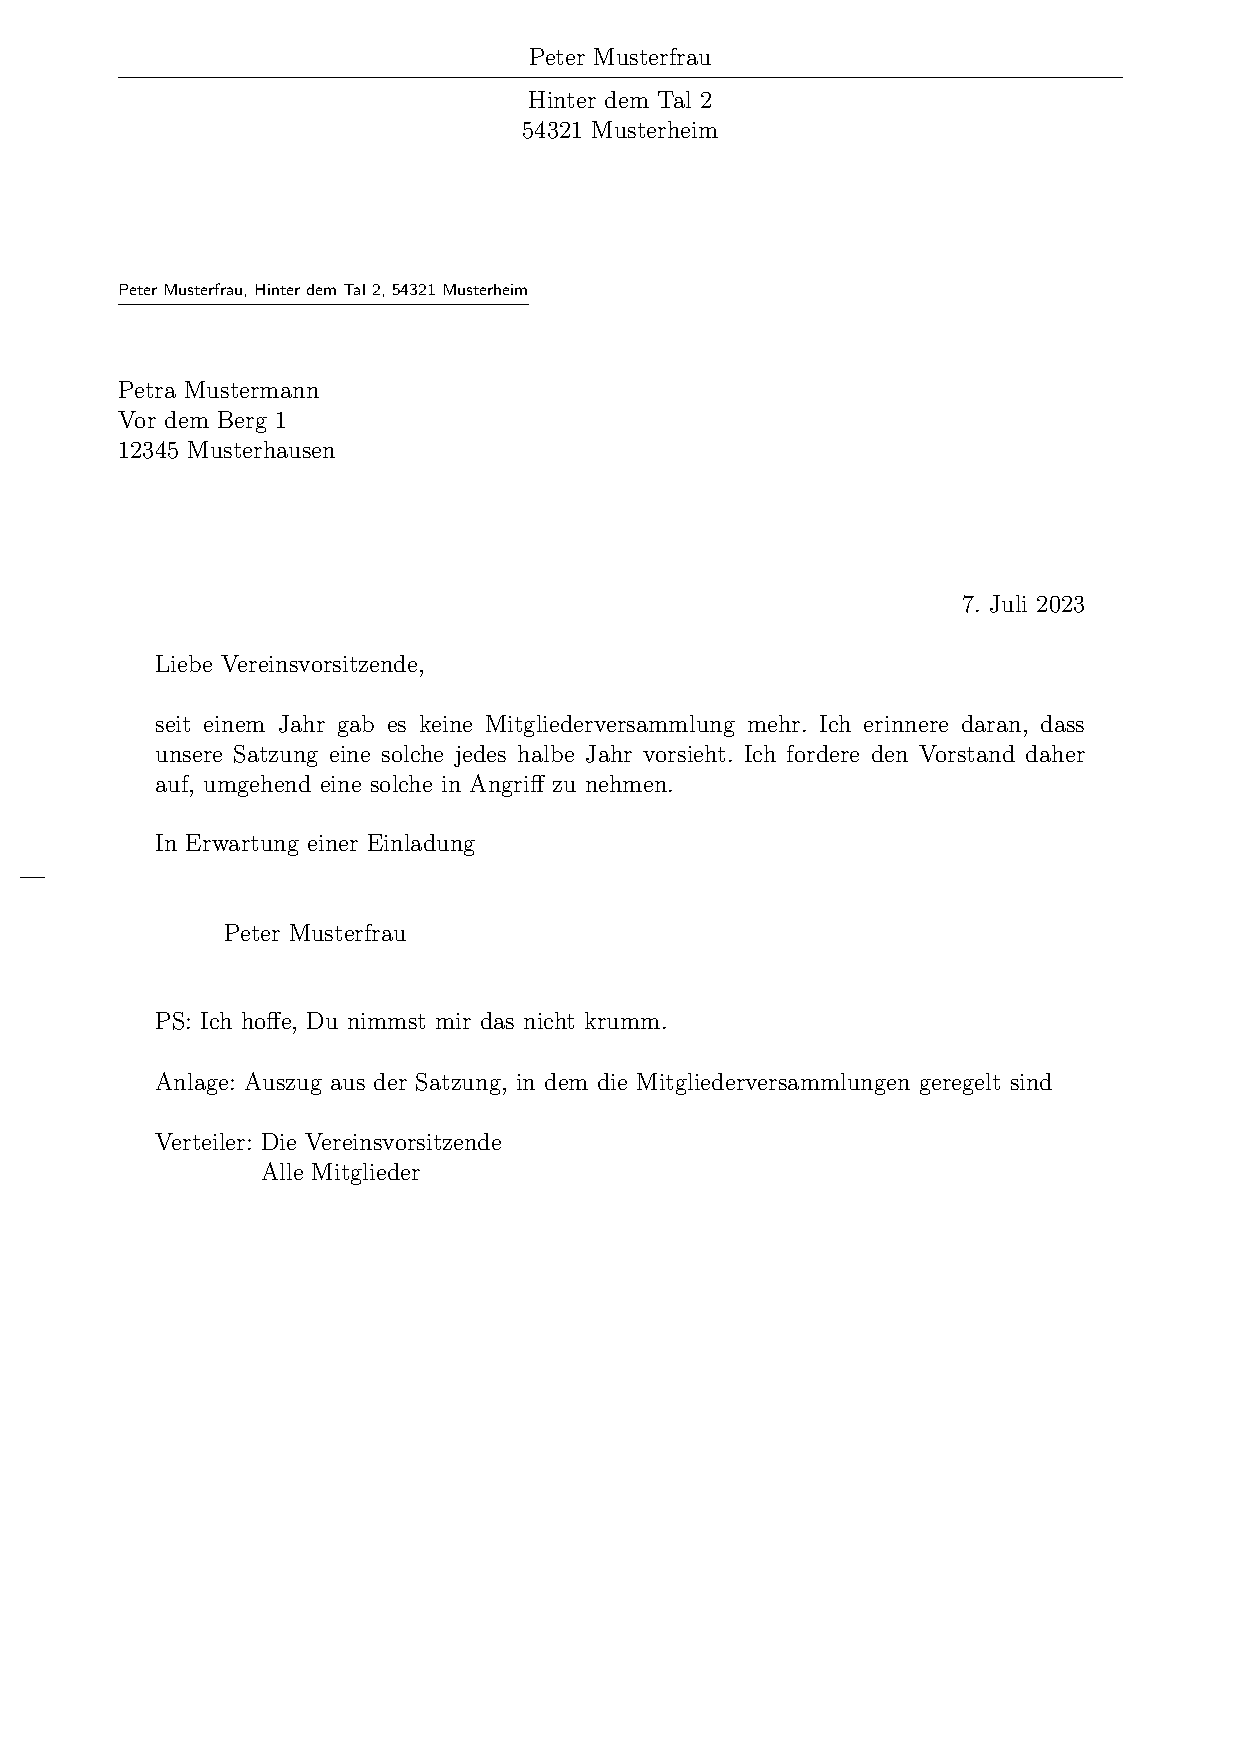
\includegraphics[width=.4\textwidth]{letter-example-08-de}}\quad
    \frame{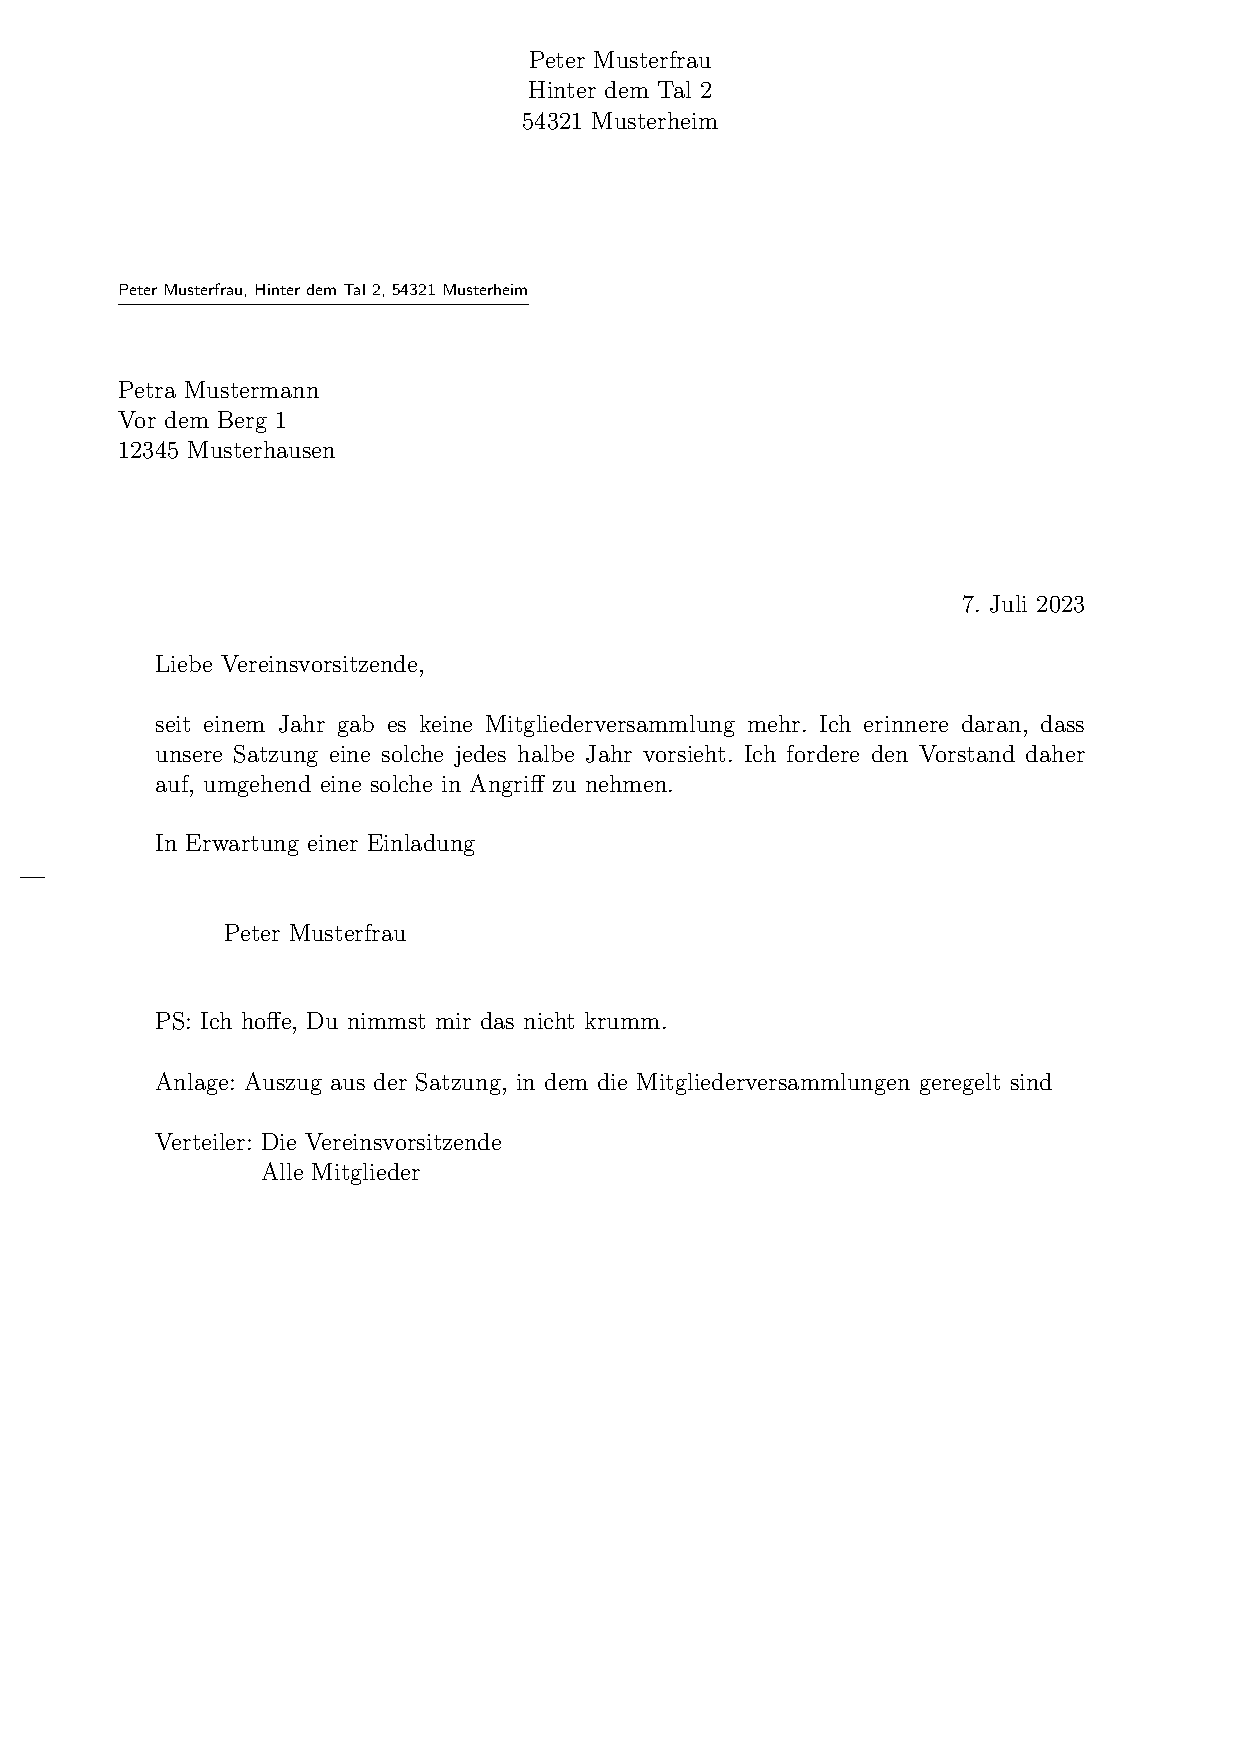
\includegraphics[width=.4\textwidth]{letter-example-09-de}}
    \caption[{Beispiel: Brief mit Absender, Anschrift, Anrede,
      Text, Grußfloskel, Signatur, Postskriptum, Anlagen und Verteiler}]
    {Ergebnis eines kleinen Briefes mit Absender, Anschrift, Anrede, Text,
      Grußfloskel, Signatur, Postskriptum, Anlagen und Verteiler (Datum und
      Faltmarken entstammen den Voreinstellungen für DIN-Briefe); links der
      einfache Briefkopf mit \OptionValueRef{\LabelBase}{fromalign}{false},
      rechts der
      erweiterte Briefkopf mit \OptionValueRef{\LabelBase}{fromalign}{center}}
    \label{fig:\LabelBase.letter-8-9}
  \end{figure}
  Dabei wird zunächst %
  \iffalse % Umbruchkorrektur
  einmal nicht der erweiterte Briefkopf, sondern %
  \fi %
  nur der einfache Briefkopf verwendet. Das Ergebnis ist in
  \autoref{fig:\LabelBase.letter-8-9} links zu sehen.  Im Vergleich dazu ist
  rechts daneben das gleiche Beispiel, jedoch mit Option
  \OptionValueRef{\LabelBase}{fromalign}{center}, also mit den aktivierten
  Erweiterungen für den Briefkopf, abgebildet. Wie zu sehen ist, hat diese
  Variante zunächst einmal keine Linie.

  In \autoref{fig:\LabelBase.letter-8-9} taucht nun auch erstmals eine Signatur
  unter dem Gruß auf. Diese wird automatisch aus dem Absendername
  gewonnen. Wie sie konfiguriert werden kann, ist in
  \autoref{sec:\LabelBase.closing} ab \autopageref{sec:\LabelBase.closing} zu
  finden.

  Nun soll der Brief mit aktivierter Erweiterung für den Briefkopf mit Hilfe
  der Option \Option{fromrule} auch noch eine Linie unter dem Namen erhalten:%
  \lstinputcode[xleftmargin=1em]{letter-example-11-de.tex}%
  Das Ergebnis ist in \autoref{fig:\LabelBase.letter-10-11} rechts zu sehen. %
  \iffalse % Umbruchkorrektur
  Im Vergleich dazu ist links daneben das gleiche Beispiel noch einmal mit dem
  einfachen Briefkopf und ohne Reaktion auf die zusätzliche Option.
  % 
  \else %
  Links steht zum Vergleich ein Beispiel mit dem einfachen Briefkopf.
  %
  \fi 
  %
  \begin{figure}
    \centering
    \frame{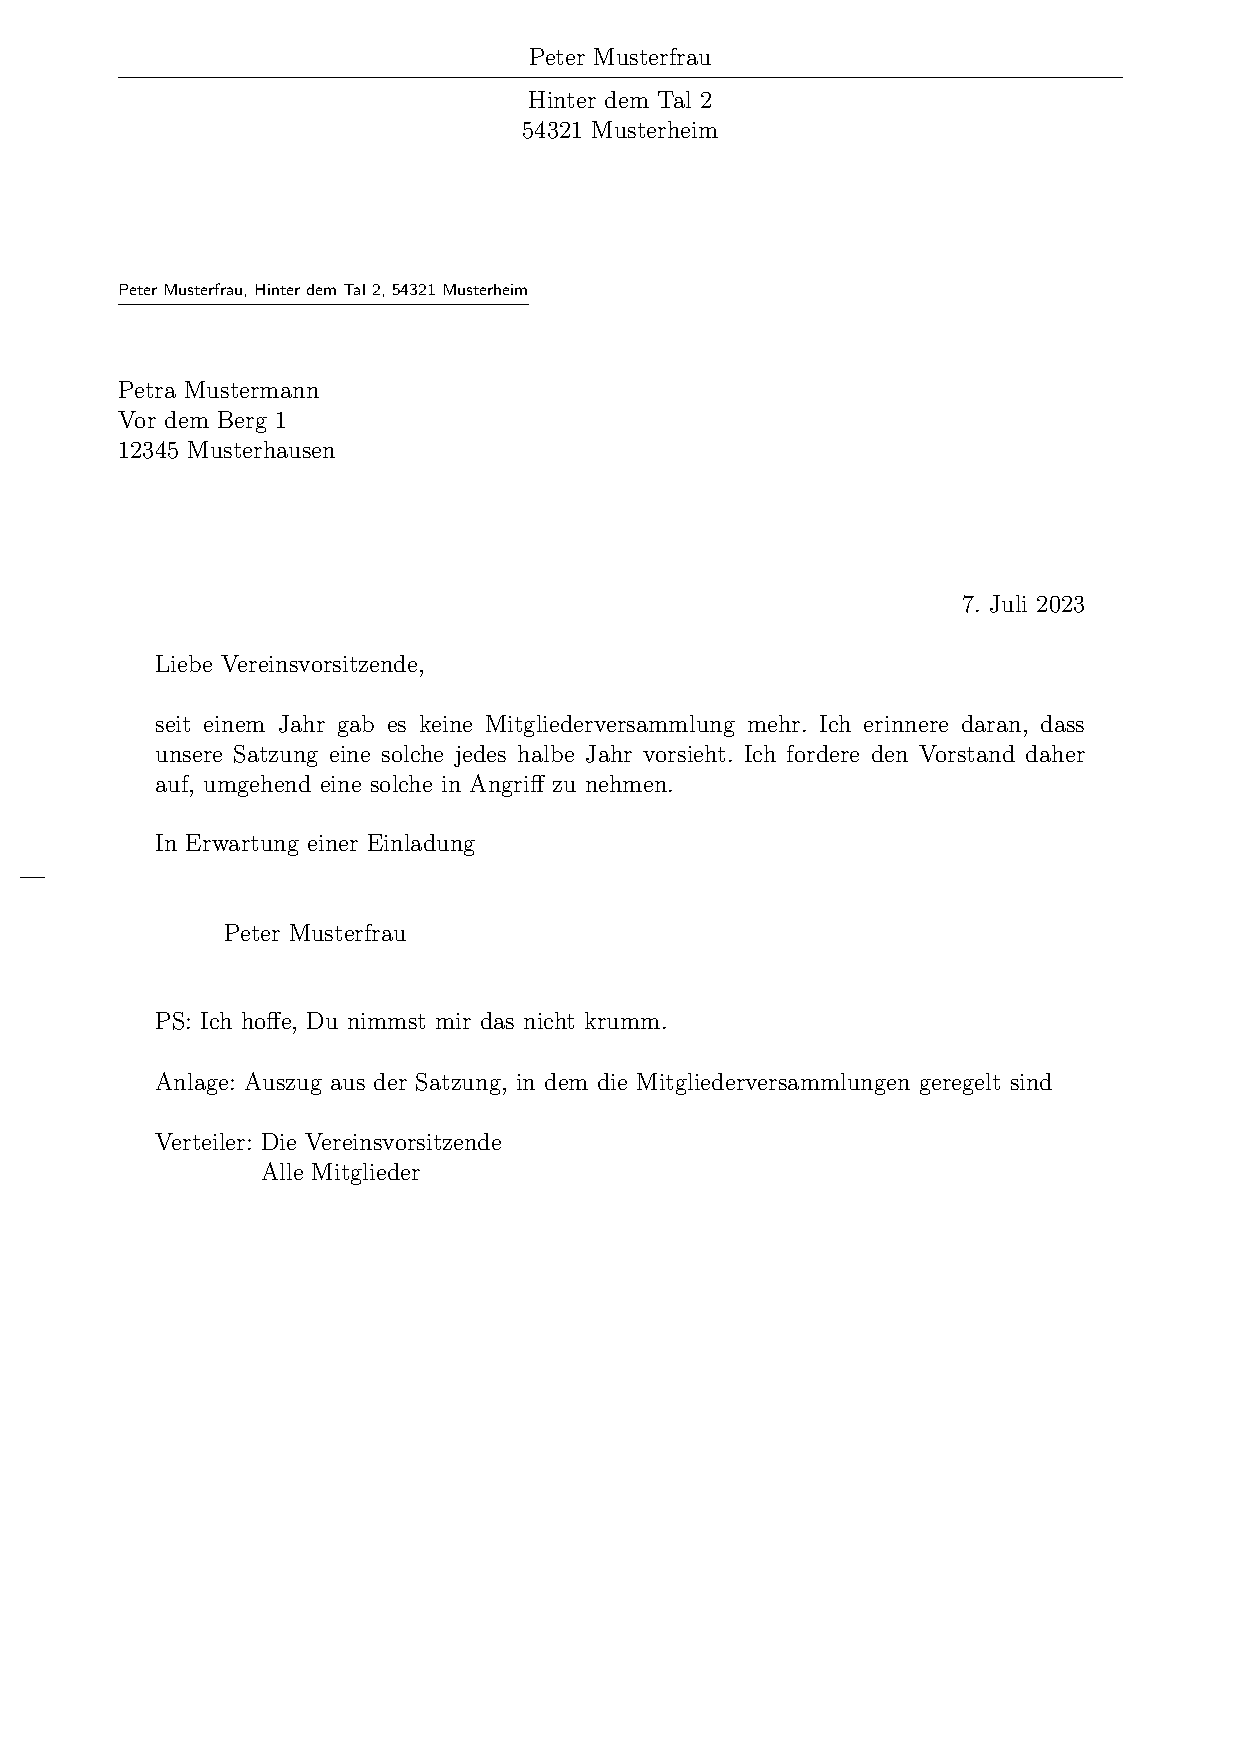
\includegraphics[width=.4\textwidth]{letter-example-10-de}}\quad
    \frame{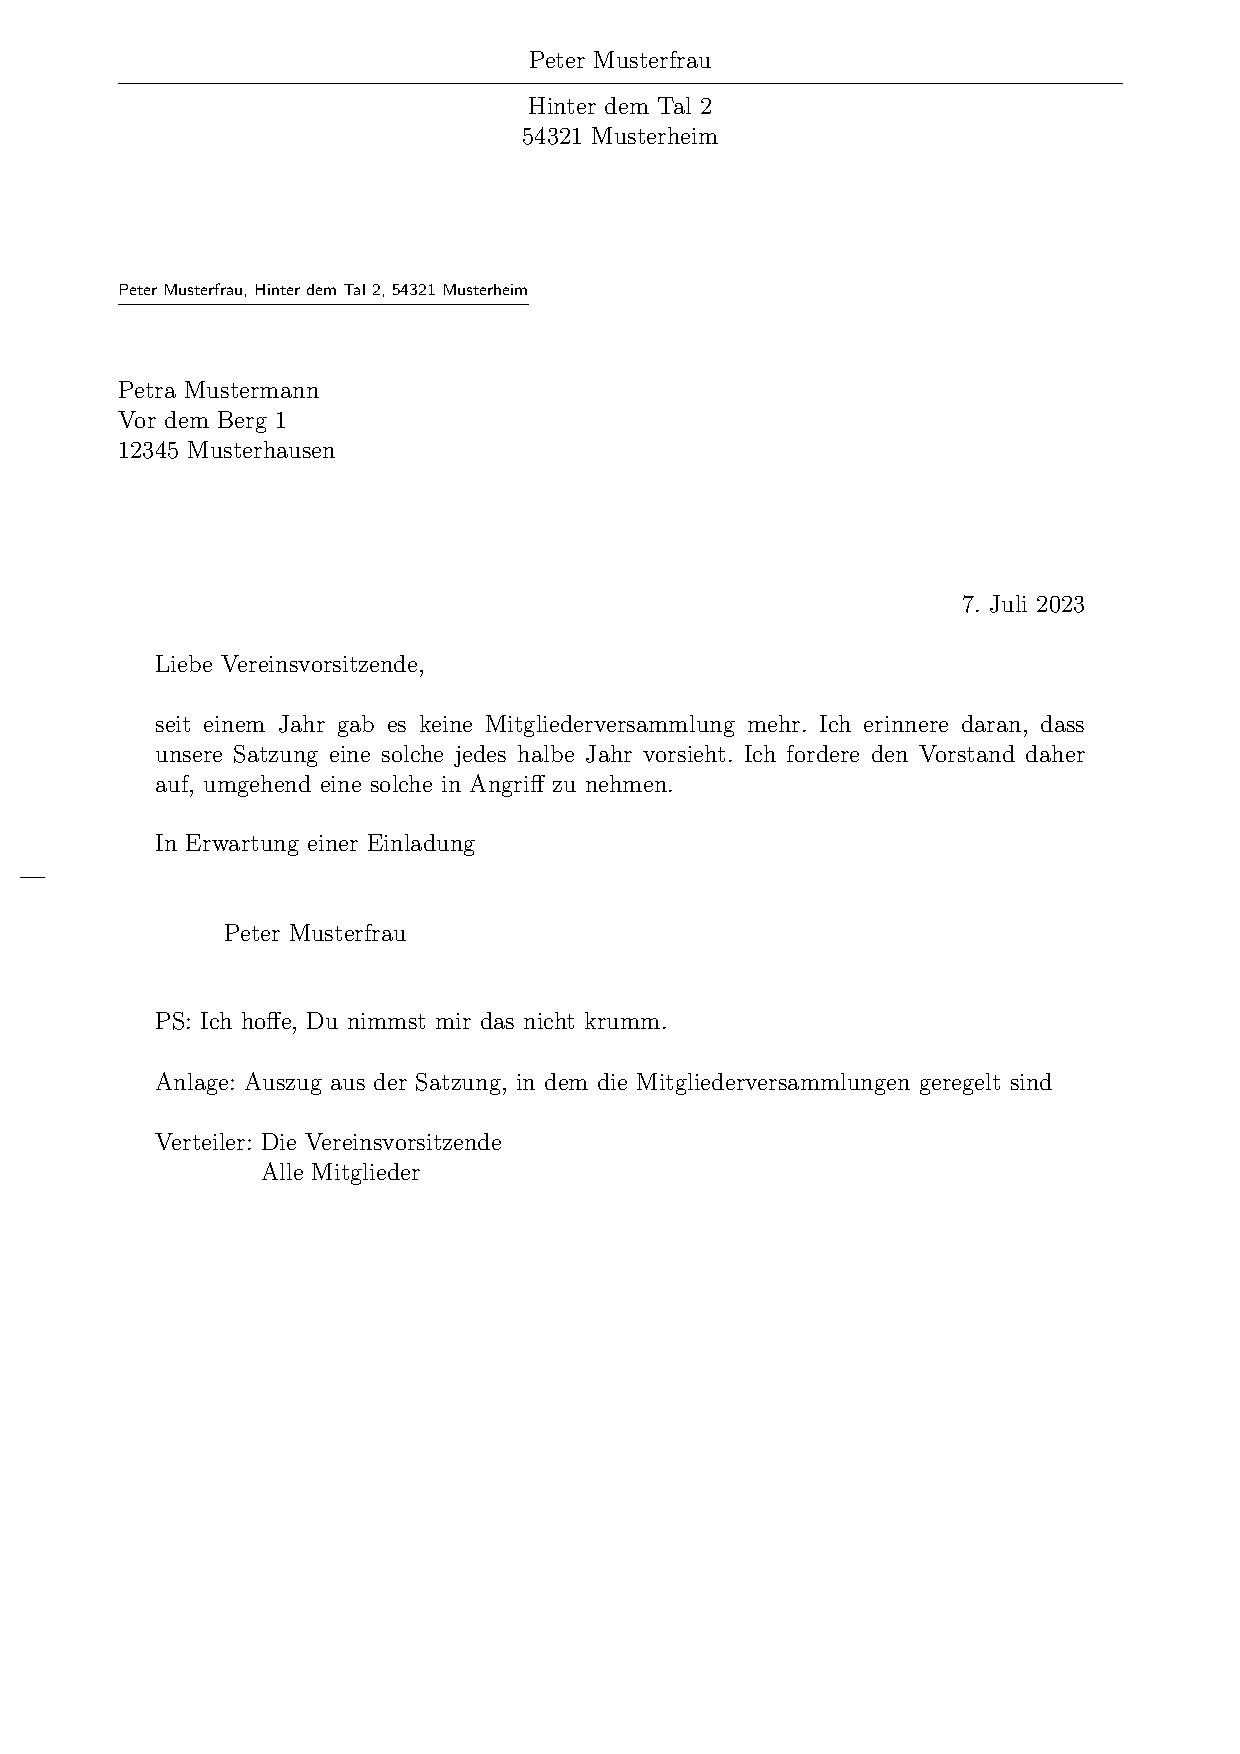
\includegraphics[width=.4\textwidth]{letter-example-11-de}}
    \caption[{Beispiel: Brief mit Absender, Trennlinie, Anschrift, Anrede, Text,
      Grußfloskel, Signatur, Postskriptum, Anlagen, Verteiler und
      Lochermarke}]{Ergebnis eines kleinen Briefes mit Absender, Trennlinie,
      Anschrift, Anrede, Text, Grußfloskel, Signatur, Postskriptum, Anlagen,
      Verteiler und Lochermarke (das Datum entstammt den Voreinstellungen für
      DIN-Briefe); links der einfache Briefkopf mit
      \OptionValueRef{\LabelBase}{fromalign}{false}, rechts der erweiterte
      Briefkopf mit \OptionValueRef{\LabelBase}{fromalign}{center}}
    \label{fig:\LabelBase.letter-10-11}
  \end{figure}
\end{Example}

Ein\textnote{Achtung!} wichtiger Hinweis betrifft \iffree{noch}{\unskip} die
Absenderadresse: Innerhalb der Absenderadresse werden einzelne Teilangaben
durch doppelten Backslash voneinander getrennt. Solche Teilangaben sind
beispielsweise Straße und Hausnummer, Postleitzahl und Ort oder eine
Länderangabe. Dieser doppelte Backslash wird je nach Verwendung der
Absenderadresse unterschiedlich interpretiert und ist nicht zwangsläufig als
Zeilenumbruch zu verstehen.  Absätze, vertikale Abstände und Ähnliches sind
innerhalb der Absenderangaben normalerweise nicht gestattet%
\iffalse % Umbruchkorrektur
. Man muss \KOMAScript{} schon sehr genau kennen, um solche Mittel
gegebenenfalls sinnvoll im Absender einsetzen zu können.  Außerdem sollte man
in dem Fall unbedingt die Variablen für Rücksendeadresse (siehe Variable
\DescRef{\LabelBase.variable.backaddress},
\DescPageRef{\LabelBase.variable.backaddress}) und Signatur (siehe Variable
\DescRef{\LabelBase.variable.signature},
\DescPageRef{\LabelBase.variable.signature}) selbst setzen.%
\else %
\ und hätten außerdem gegebenenfalls Auswirkungen auf die Rücksendeadresse
(siehe Variable \DescRef{\LabelBase.variable.backaddress},
\DescPageRef{\LabelBase.variable.backaddress}) und Signatur (siehe Variable
\DescRef{\LabelBase.variable.signature},
\DescPageRef{\LabelBase.variable.signature}).%
\fi %
%
\EndIndexGroup


\begin{Declaration}
  \PLength{fromrulethickness}
  \PLength{fromrulewidth}
\end{Declaration}
Wie bereits bei Option
\DescRef{\LabelBase.option.fromrule}\IndexOption{fromrule} auf
\DescPageRef{\LabelBase.option.fromrule} erwähnt wurde, kann in den
vordefinierten Briefköpfen eine Linie im oder unter dem Absender gesetzt
werden. Hat\textnote{Achtung!} die Pseudolänge \PLength{fromrulewidth} die
Länge 0, so wird dabei die Länge dieser Linie automatisch bestimmt. Dies ist
die Voreinstellung\textnote{Voreinstellung} bei den vordefinierten
\File{lco}-Dateien. %
\iffalse % Umbruchkorrekturtext
Der Wert kann mit \DescRef{\LabelBase.cmd.setplength} (siehe
\DescPageRef{\LabelBase.cmd.setplength}) in eigenen \File{lco}-Dateien aber
auch abweichend gesetzt werden. %
\fi%
Die voreingestellte Dicke\ChangedAt{v2.97c}{\Class{scrlttr2}},
\PLength{fromrulethickness}, der Linie beträgt 0,4\Unit{pt}.%
\EndIndexGroup


\begin{Declaration}
  \OptionVName{symbolicnames}{Wert}
  \OptionVName{fromphone}{Ein-Aus-Wert}
  \OptionVName{frommobilephone}{Ein-Aus-Wert}
  \OptionVName{fromfax}{Ein-Aus-Wert}
  \OptionVName{fromemail}{Ein-Aus-Wert}
  \OptionVName{fromurl}{Ein-Aus-Wert}
  \Variable{fromphone}
  \Variable{frommobilephone}
  \Variable{fromfax}
  \Variable{fromemail}
  \Variable{fromurl}
  \Variable{phoneseparator}
  \Variable{mobilephoneseparator}
  \Variable{faxseparator}
  \Variable{emailseparator}
  \Variable{urlseparator}
\end{Declaration}%
Mit Hilfe der fünf Optionen \Option{fromphone},
\Option{frommobilephone}\ChangedAt{v3.12}{\Class{scrlttr2}}, \Option{fromfax},
\Option{fromemail} und \Option{fromurl} kann bestimmt werden, ob die
Telefonnummer\Index{Telefon}, die
Mobiltelefonnummer\Index{Mobiltelefon}\Index{Handy}, die Faxnummer\Index{Fax},
die E-Mail-Adresse und die URL im Absender\Index{Absender} gesetzt werden
soll. Als \PName{Ein-Aus-Wert} kann dabei einer der Standardwerte für einfache
Schalter aus \autoref{tab:truefalseswitch}, \autopageref{tab:truefalseswitch}
verwendet werden. Voreingestellt\textnote{Voreinstellung} ist jeweils
\PValue{false}. Die Inhalte selbst werden über die gleichnamigen Variablen
bestimmt. Die Voreinstellungen für die dabei verwendeten Bezeichnungen sind
\autoref{tab:\LabelBase.fromTerm} zu entnehmen, die verwendeten Trennzeichen,
die zwischen der \PName{Bezeichnung} und dem \PName{Inhalt} einer Variablen
eingefügt werden, \autoref{tab:\LabelBase.fromSeparator}.

Mit\ChangedAt{v3.12}{\Class{scrlttr2}}\important{\Option{symbolicnames}}
Option \Option{symbolicnames} kann diese Voreinstellung auf einen Schlag
geändert werden. Die Option versteht die
Ein-Aus-Werte für einfache Schalter, wie sie in
\autoref{tab:truefalseswitch}, \autopageref{tab:truefalseswitch} angegeben
sind. Die\ChangedAt{v3.27}{\Class{scrlttr2}\and \Package{scrletter}}
Aktivierung der Option entspricht dabei dem \PName{Wert} \PValue{marvosym},
wodurch statt der sprachabhängigen Bezeichner
\DescRef{scrlttr2-experts.cmd.emailname},
\DescRef{scrlttr2-experts.cmd.faxname},
\DescRef{scrlttr2-experts.cmd.mobilephonename} und
\DescRef{scrlttr2-experts.cmd.phonename} Symbole aus dem
\Package{marvosym}\IndexPackage{marvosym}-Paket verwendet werden. Gleichzeitig
entfällt der Doppelpunkt bei der Definition der Trennzeichen. Für die URL
entfallen in diesem Fall sowohl der sprachabhängige Bezeichner als auch das
Trennzeichen. Mit \OptionValue{symbolicnames}{fontawesome} oder
\OptionValue{symbolicnames}{awesome} werden stattdessen Symbole von Paket
\Package{fontawesome}\IndexPackage{fontawesome} verwendet. Dabei wird auch für
die URL ein passendes Symbol aktiviert. Es ist zu beachten\textnote{Achtung!},
dass das Paket \Package{marvosym} oder \Package{fontawesome} gegebenenfalls
selbst in der Dokumentpräambel zu laden ist, falls mit der Option erst nach
\Macro{begin}\PParameter{document} die Verwendung eines dieser Pakete
aktiviert wird.

\begin{table}
  \centering
  \caption[{Vordefinierte Bezeichnungen der Variablen für die\newline
    Absenderangaben im Briefkopf}]{Vordefinierte Bezeichnungen der Variablen
    für die Absenderangaben im Briefkopf (die Bezeichnungen und Inhalte der
    verwendeten Variablen für Trennzeichen sind
    \autoref{tab:\LabelBase.fromSeparator} zu entnehmen)}
  \begin{desctabular}[1.8em]
    \ventry{fromemail}{%
      \DescRef{\LabelBase.cmd.usekomavar*}\PParameter{emailseparator}%
      \DescRef{\LabelBase.cmd.usekomavar}\PParameter{emailseparator}}%
    \ventry{fromfax}{%
      \DescRef{\LabelBase.cmd.usekomavar*}\PParameter{faxseparator}%
      \DescRef{\LabelBase.cmd.usekomavar}\PParameter{faxseparator}}%
    \ventry{frommobilephone}{%
      \DescRef{\LabelBase.cmd.usekomavar*}\PParameter{mobilephoneseparator}%
      \DescRef{\LabelBase.cmd.usekomavar}\PParameter{mobilephoneseparator}}%
    \ventry{fromname}{\DescRef{scrlttr2-experts.cmd.headfromname}}%
    \ventry{fromphone}{%
      \DescRef{\LabelBase.cmd.usekomavar*}\PParameter{phoneseparator}%
      \DescRef{\LabelBase.cmd.usekomavar}\PParameter{phoneseparator}}%
    \ventry{fromurl}{%
      \DescRef{\LabelBase.cmd.usekomavar*}\PParameter{urlseparator}%
      \DescRef{\LabelBase.cmd.usekomavar}\PParameter{urlseparator}}%
  \end{desctabular}
  \label{tab:\LabelBase.fromTerm}
\end{table}

\begin{table}[tp]
  \centering
%  \KOMAoptions{captions=topbeside}%
%  \setcapindent{0pt}%
  \caption
%  \begin{captionbeside}
  {Vordefinierte Bezeichnungen und Inhalte der Trennzeichen
    für die Absenderangaben im Briefkopf ohne Option
    \Option{symbolicnumbers}}
%    [l]
  \begin{tabularx}{\textwidth}{llX}
    \toprule
    Name                      & Bezeichnung & Inhalt \\
    \midrule
    \Variable{emailseparator} & \DescRef{scrlttr2-experts.cmd.emailname} & \texttt{:\~} \\
    \Variable{faxseparator}   & \DescRef{scrlttr2-experts.cmd.faxname}   & \texttt{:\~} \\
    \Variable{mobilephoneseparator} & \DescRef{scrlttr2-experts.cmd.mobilephonename} &
                   \DescRef{\LabelBase.cmd.usekomavar}\PParameter{phoneseparator} \\
    \Variable{phoneseparator} & \DescRef{scrlttr2-experts.cmd.phonename} & \texttt{:\~} \\
    \Variable{urlseparator}   & \DescRef{scrlttr2-experts.cmd.wwwname}   & \texttt{:\~} \\
    \bottomrule
  \end{tabularx}
%  \end{captionbeside}
  \label{tab:\LabelBase.fromSeparator}
\end{table}

\begin{Example}
  Herr Musterfrau aus unserem Beispiel hat auch Telefon und eine
  E-Mail-Adresse. Diese möchte er ebenfalls im Briefkopf haben. Gleichzeitig
  soll die Trennlinie nun nach dem Briefkopf stehen. Also gibt er die
  entsprechenden Optionen an und setzt auch die zugehörigen Variablen:%
  \lstinputcode[xleftmargin=1em]{letter-example-12-de.tex}%
  Das Ergebnis aus \autoref{fig:\LabelBase.letter-12-13} links ist jedoch
  ernüchternd. Die Optionen werden ignoriert. Das liegt %
  \iffalse% Umbruchkorrektur
  daran, dass diese zusätzlichen Variablen und Optionen nur im erweiterten
  Briefkopf verwendet werden. %
  \else%
  an Option \OptionValueRef{\LabelBase}{fromalign}{false}. %
  \fi%
  Es muss also, wie in \autoref{fig:\LabelBase.letter-12-13}, rechts
  beispielsweise Option \OptionValueRef{\LabelBase}{fromalign}{center}
  verwendet werden:%
  \begin{figure}
    \centering
    \frame{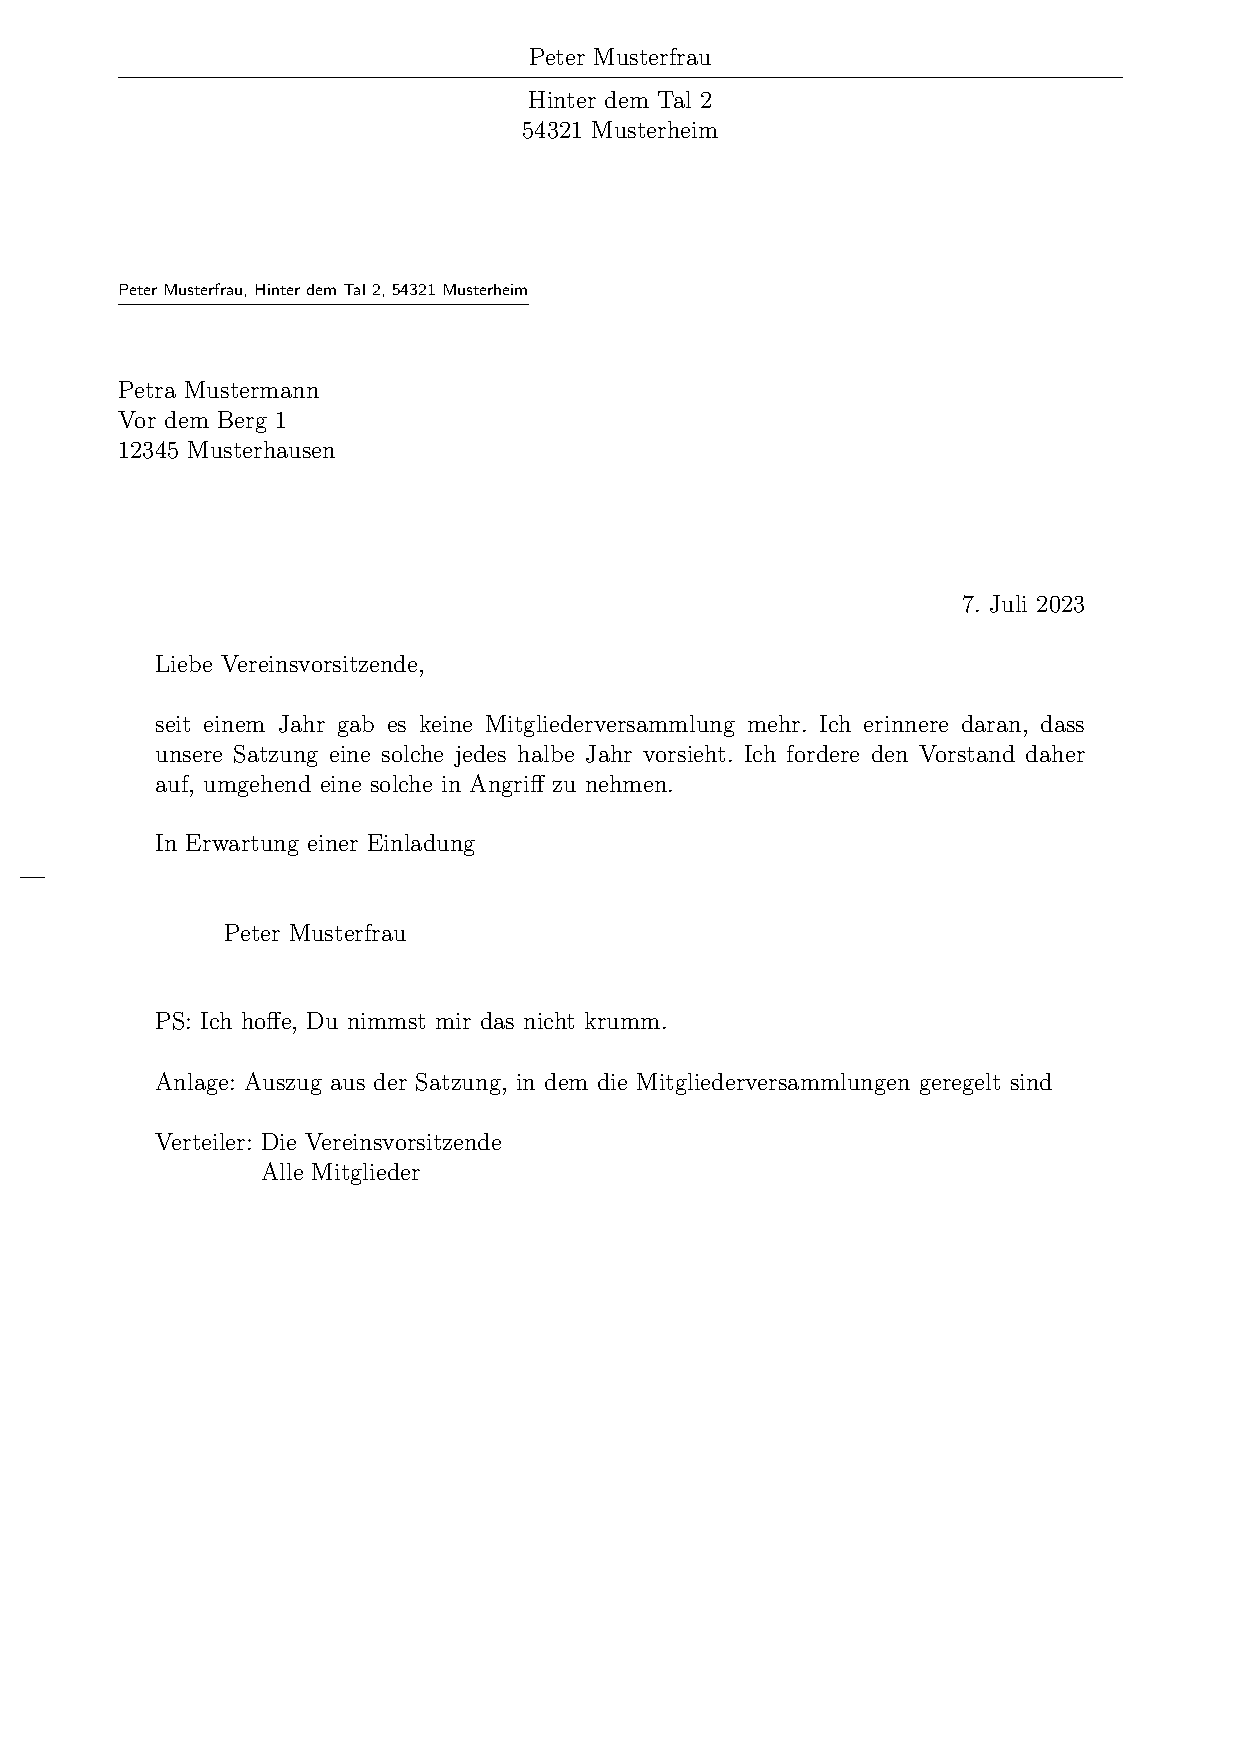
\includegraphics[width=.4\textwidth]{letter-example-12-de}}\quad
    \frame{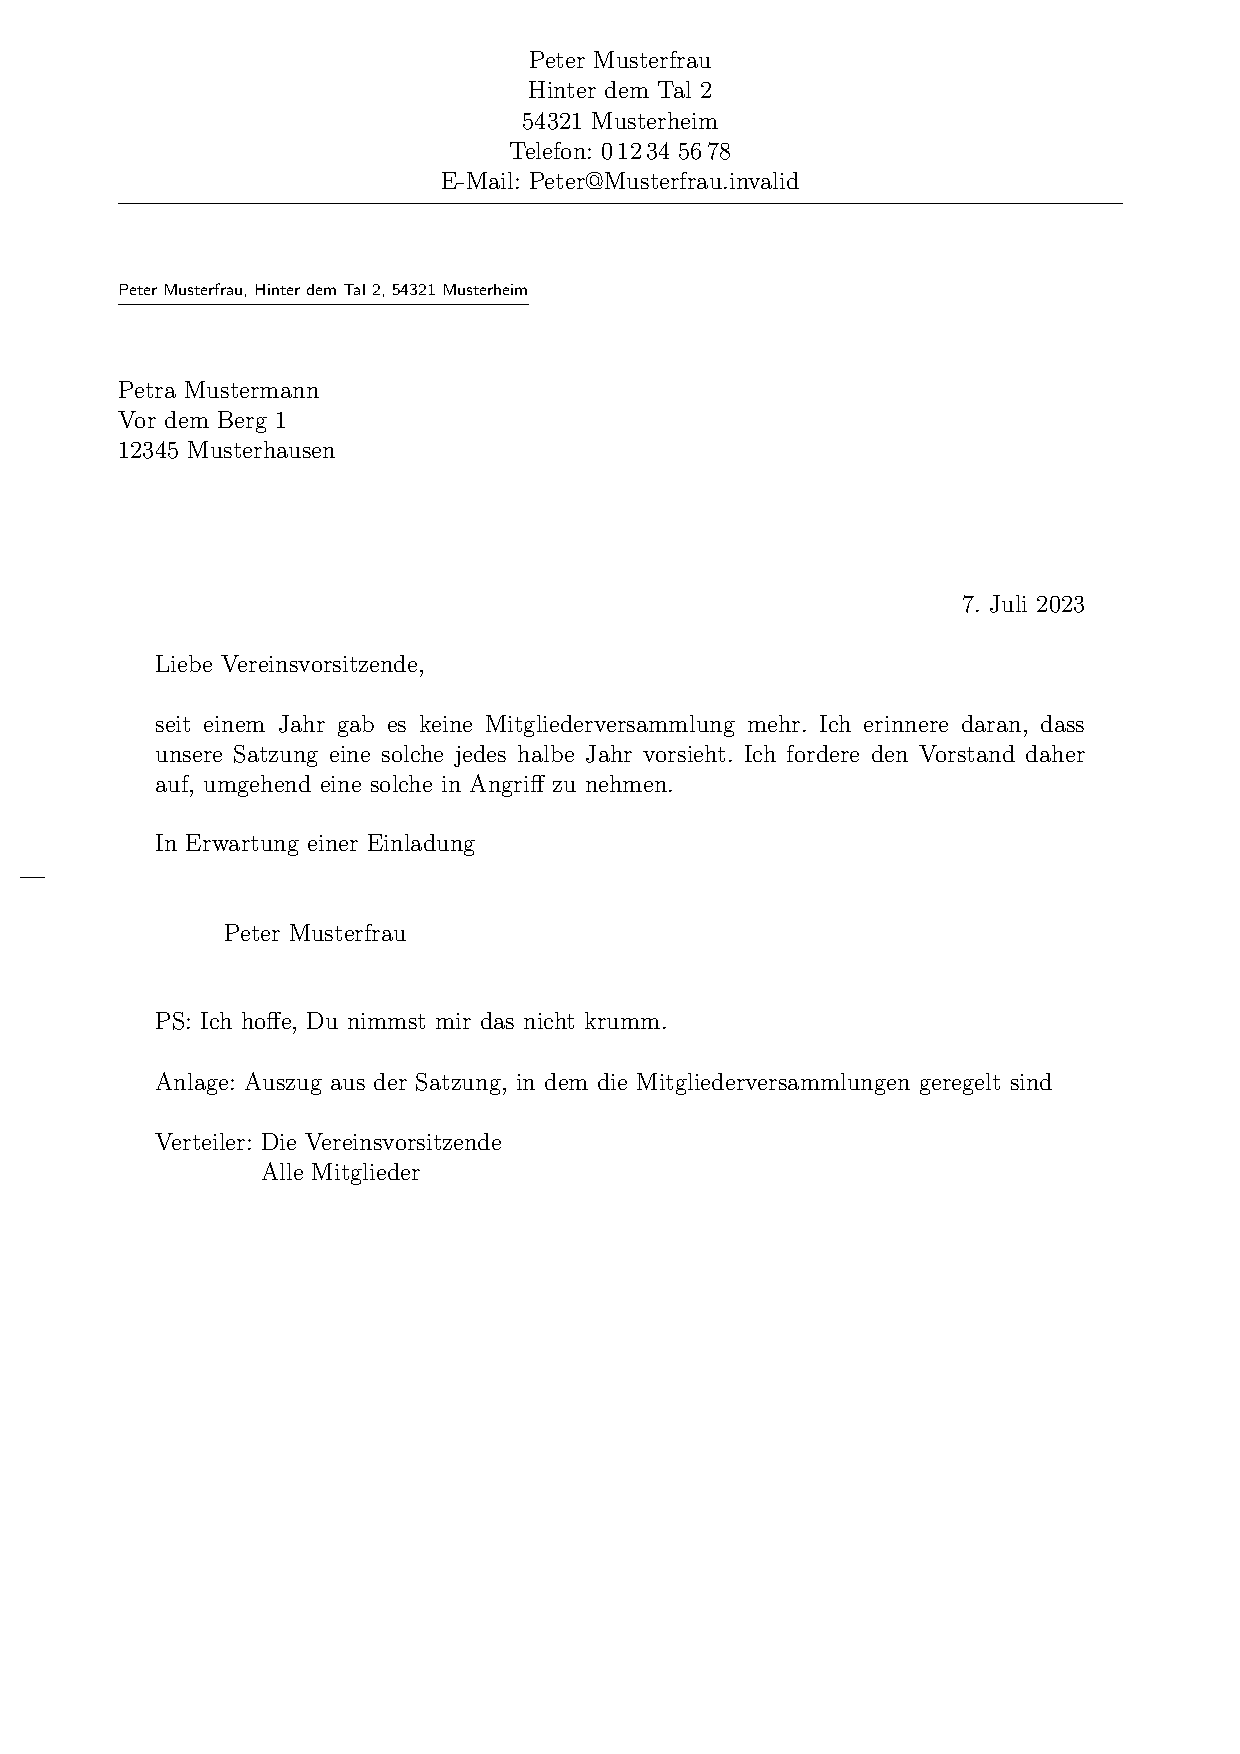
\includegraphics[width=.4\textwidth]{letter-example-13-de}}
    \caption[{Beispiel: Brief mit erweitertem Absender, Trennlinie, Anschrift,
      Anrede, Text, Grußfloskel, Signatur, Postskriptum, Anlagen, Verteiler
      und Lochermarke; Standard- vs. erweiterter Briefkopf}]{Ergebnis eines
      kleinen Briefes mit erweitertem Absender, Trennlinie, Anschrift, Anrede,
      Text, Grußfloskel, Signatur, Postskriptum, Anlagen, Verteiler und
      Lochermarke (das Datum entstammt den Voreinstellungen für DIN-Briefe);
      links der einfache Briefkopf mit
      \OptionValueRef{\LabelBase}{fromalign}{false}, rechts der erweiterte
      Briefkopf mit \OptionValueRef{\LabelBase}{fromalign}{center}}
    \label{fig:\LabelBase.letter-12-13}
  \end{figure}
  \lstinputcode[xleftmargin=1em]{letter-example-13-de.tex}

  Den Vergleich zweier weiterer Alternativen mit linksbündigem Absender durch
  Einstellung \OptionValueRef{\LabelBase}{fromalign}{left} und rechtsbündigem
  Absender durch Einstellung \OptionValueRef{\LabelBase}{fromalign}{right} zeigt
  \autoref{fig:\LabelBase.letter-14-15}.
  \begin{figure}
    \centering
    \frame{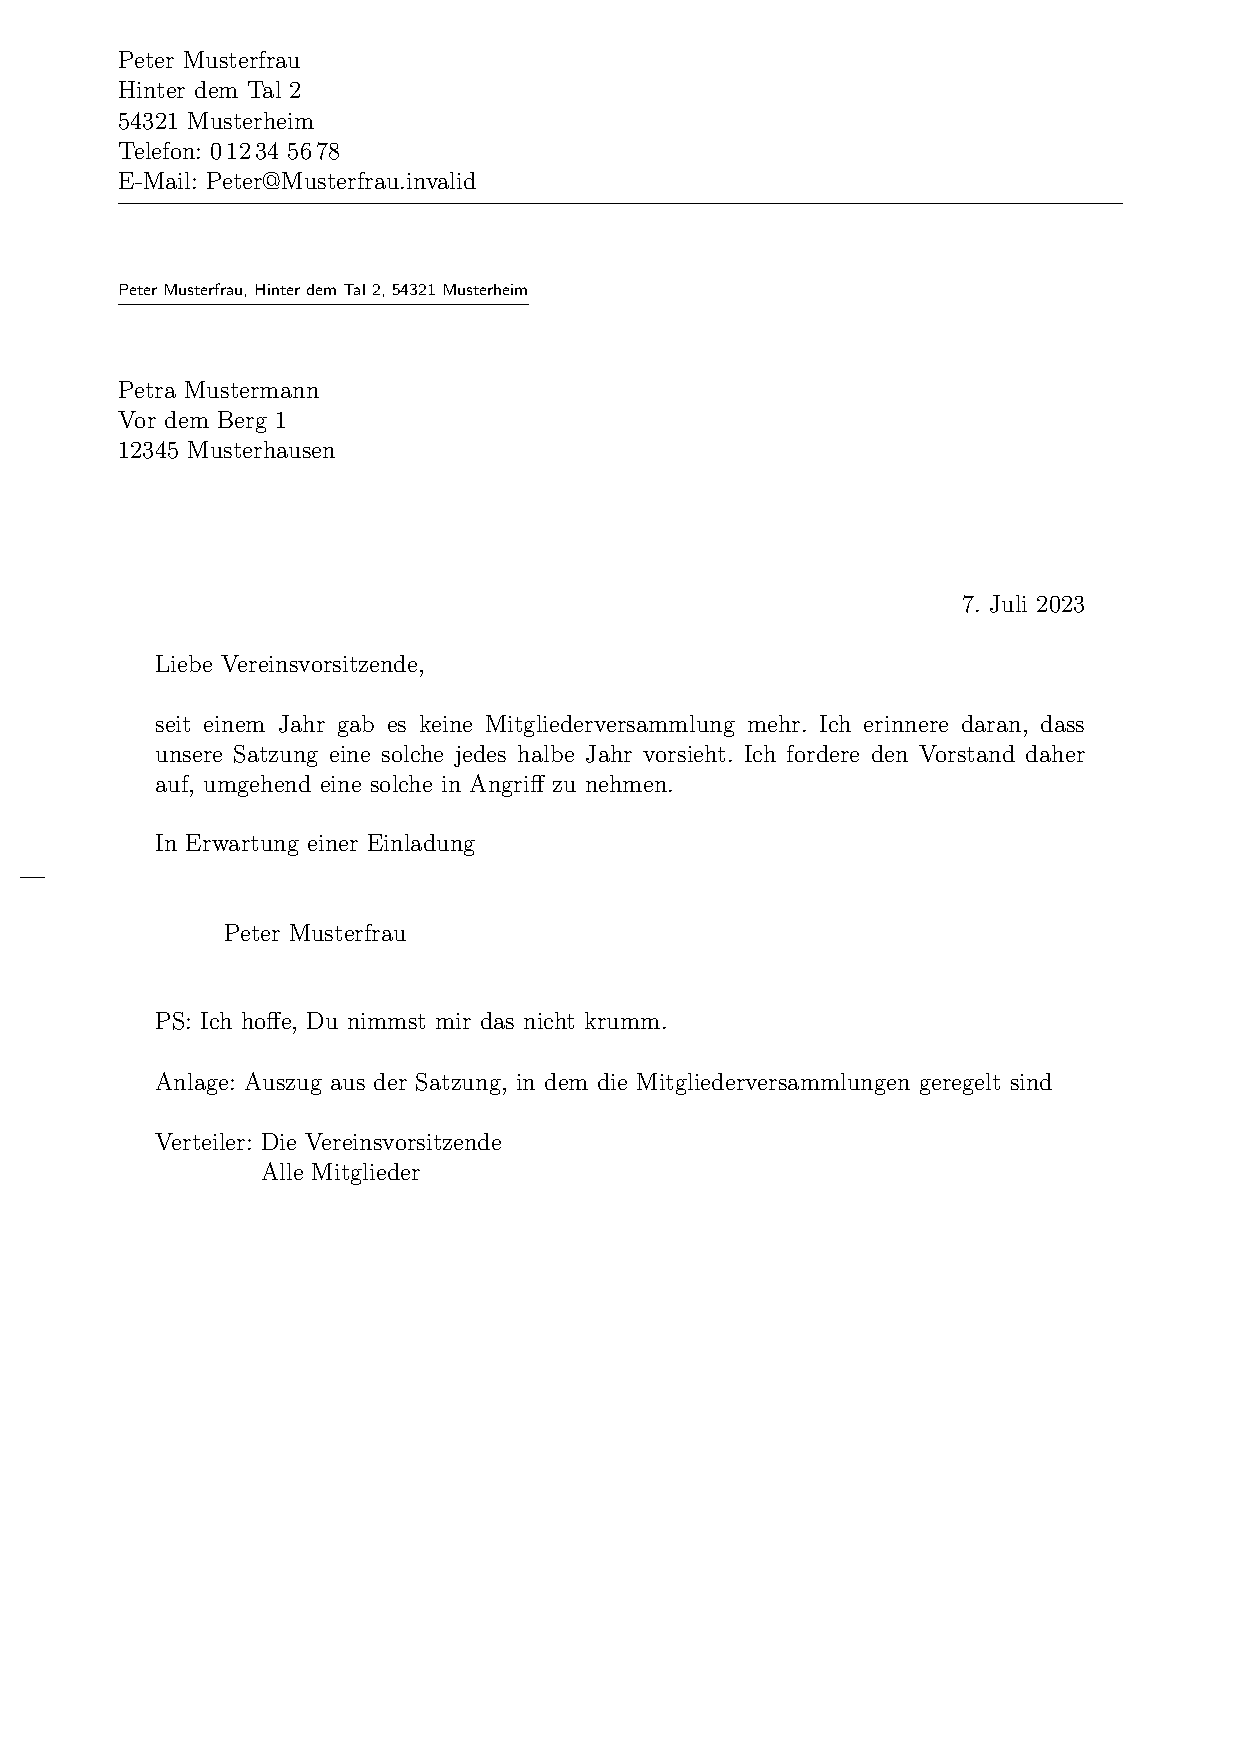
\includegraphics[width=.4\textwidth]{letter-example-14-de}}\quad
    \frame{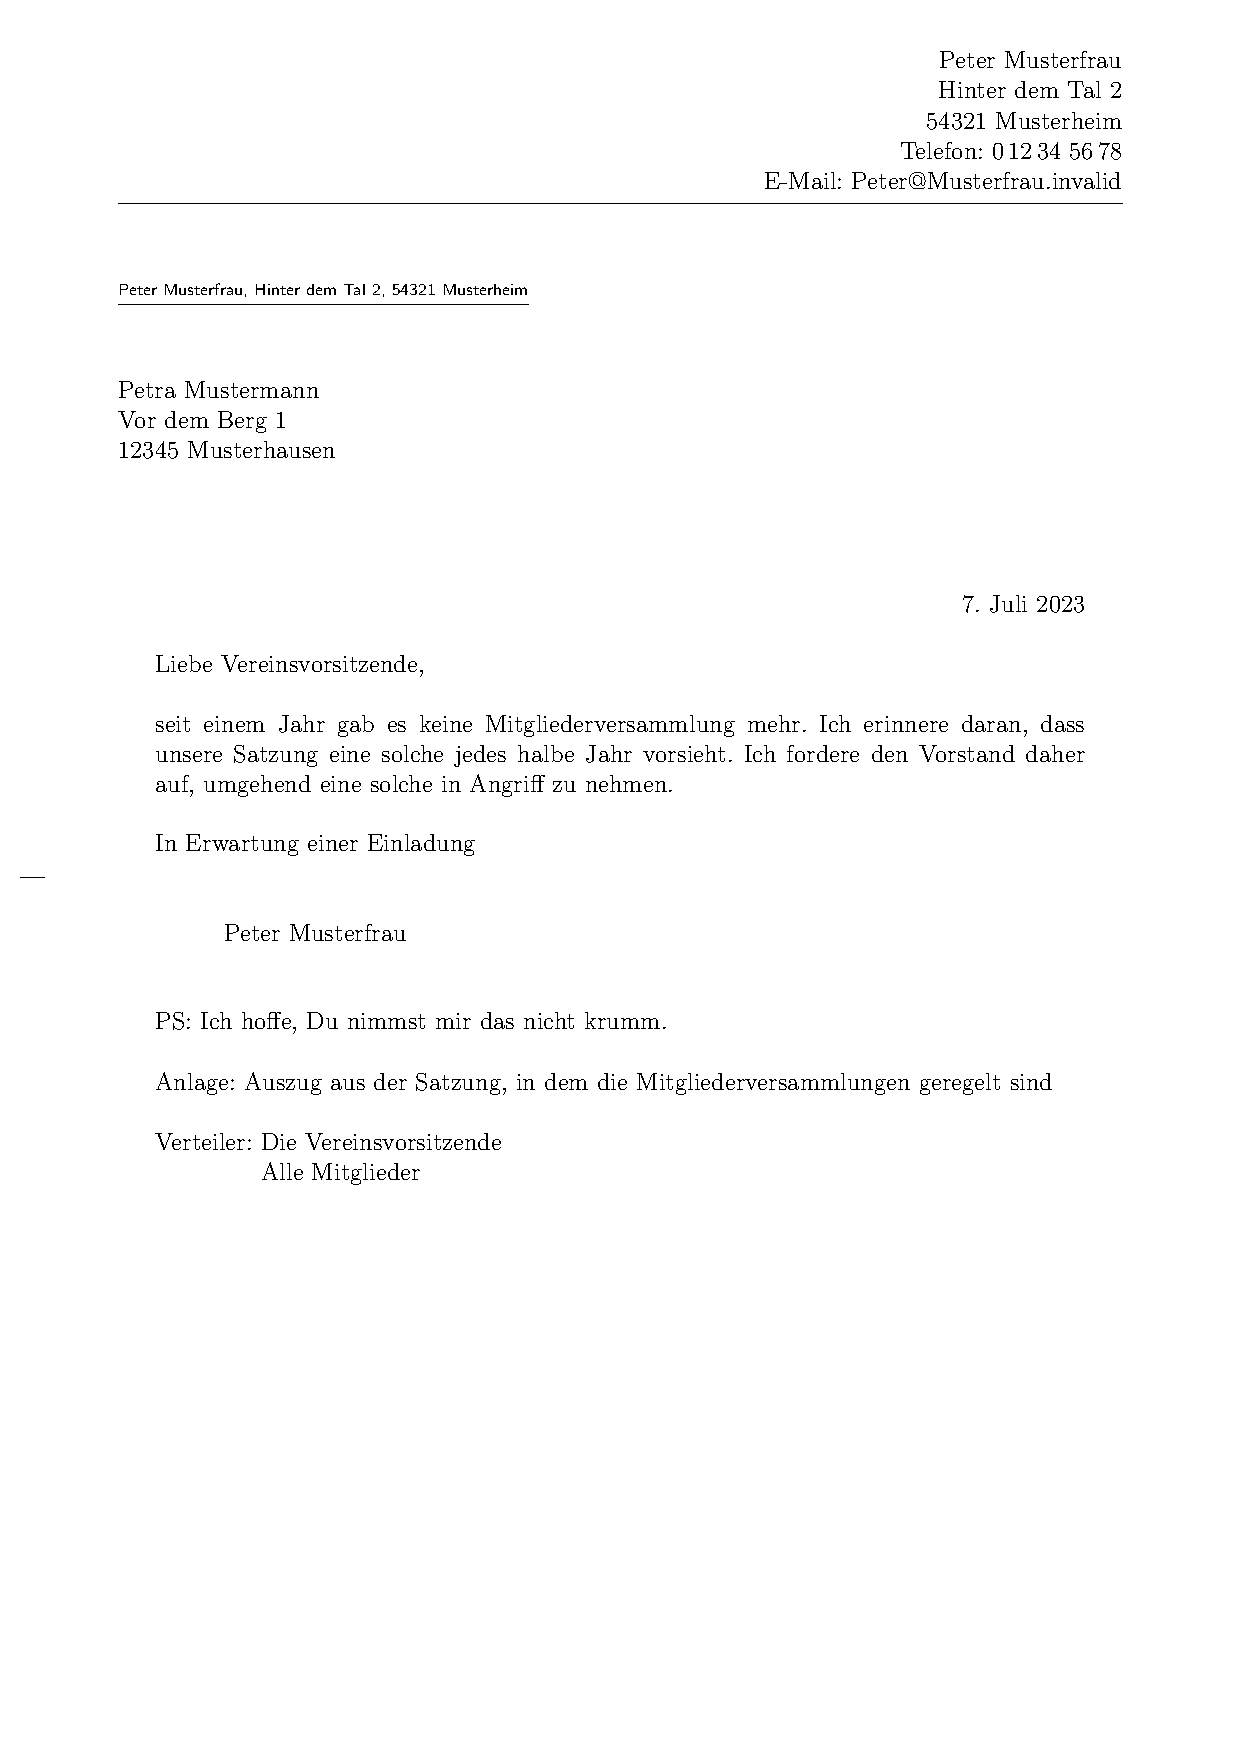
\includegraphics[width=.4\textwidth]{letter-example-15-de}}
    \caption[{Beispiel: Brief mit erweitertem Absender, Trennlinie, Anschrift,
      Anrede, Text, Grußfloskel, Signatur, Postskriptum, Anlagen, Verteiler
      und Lochermarke; links- vs. rechtsbündiger Briefkopf}]{Ergebnis eines
      kleinen Briefes mit erweitertem Absender, Trennlinie, Anschrift, Anrede,
      Text, Grußfloskel, Signatur, Postskriptum, Anlagen, Verteiler und
      Lochermarke (das Datum entstammt den Voreinstellungen für DIN-Briefe);
      links mit linksbündigem Kopf durch
      \OptionValueRef{\LabelBase}{fromalign}{left}, rechts mit Option
      \OptionValueRef{\LabelBase}{fromalign}{right} und damit rechtsbündigem
      Kopf}
    \label{fig:\LabelBase.letter-14-15}
  \end{figure}
\end{Example}
%
\EndIndexGroup
\ExampleEndFix% Beispiel am Ende


\begin{Declaration}
  \OptionVName{fromlogo}{Ein-Aus-Wert}
  \Variable{fromlogo}
\end{Declaration}
\BeginIndex{Option}{fromlogo~=\PName{Ein-Aus-Wert}}%
\BeginIndex{Variable}{fromlogo}%
Mit der Option \Option{fromlogo} kann bestimmt werden, ob ein Logo\Index{Logo}
im Briefkopf gesetzt werden soll. Als \PName{Ein-Aus-Wert} kann dabei einer
der Standardwerte für einfache Schalter aus \autoref{tab:truefalseswitch},
\autopageref{tab:truefalseswitch} verwendet
werden. Voreingestellt\textnote{Voreinstellung} ist \PValue{false}, also kein
Logo. Das Logo selbst wird über die Variable \Variable{fromlogo}
definiert. Die \PName{Bezeichnung} für das Logo ist in der Voreinstellung leer
und wird von \KOMAScript{} auch nicht verwendet.%
\begin{Example}
  Herr Musterfrau findet es besonders schick, wenn er seine Briefe mit einem
  Logo versieht. Sein Logo hat er als Grafikdatei gespeichert, die er gerne
  mit Hilfe der Anweisung \Macro{includegraphics} laden würde. Dazu bindet er
  zusätzlich das Paket \Package{graphics}\IndexPackage{graphics} (siehe
  \cite{package:graphics}) ein.%
  \lstinputcode[xleftmargin=1em]{letter-example-16-de}%
  Das Ergebnis ist in \autoref{fig:\LabelBase.letter-16-18}
  % ,\autopageref{fig:\LabelBase.letter-16-18}
  links oben zu sehen. Die beiden anderen Bilder in dieser Abbildung zeigen
  das Ergebnis bei rechtsbündigem und bei zentriertem Absender.
  \begin{figure}
     \setcapindent{0pt}%
     {\hfill
       \frame{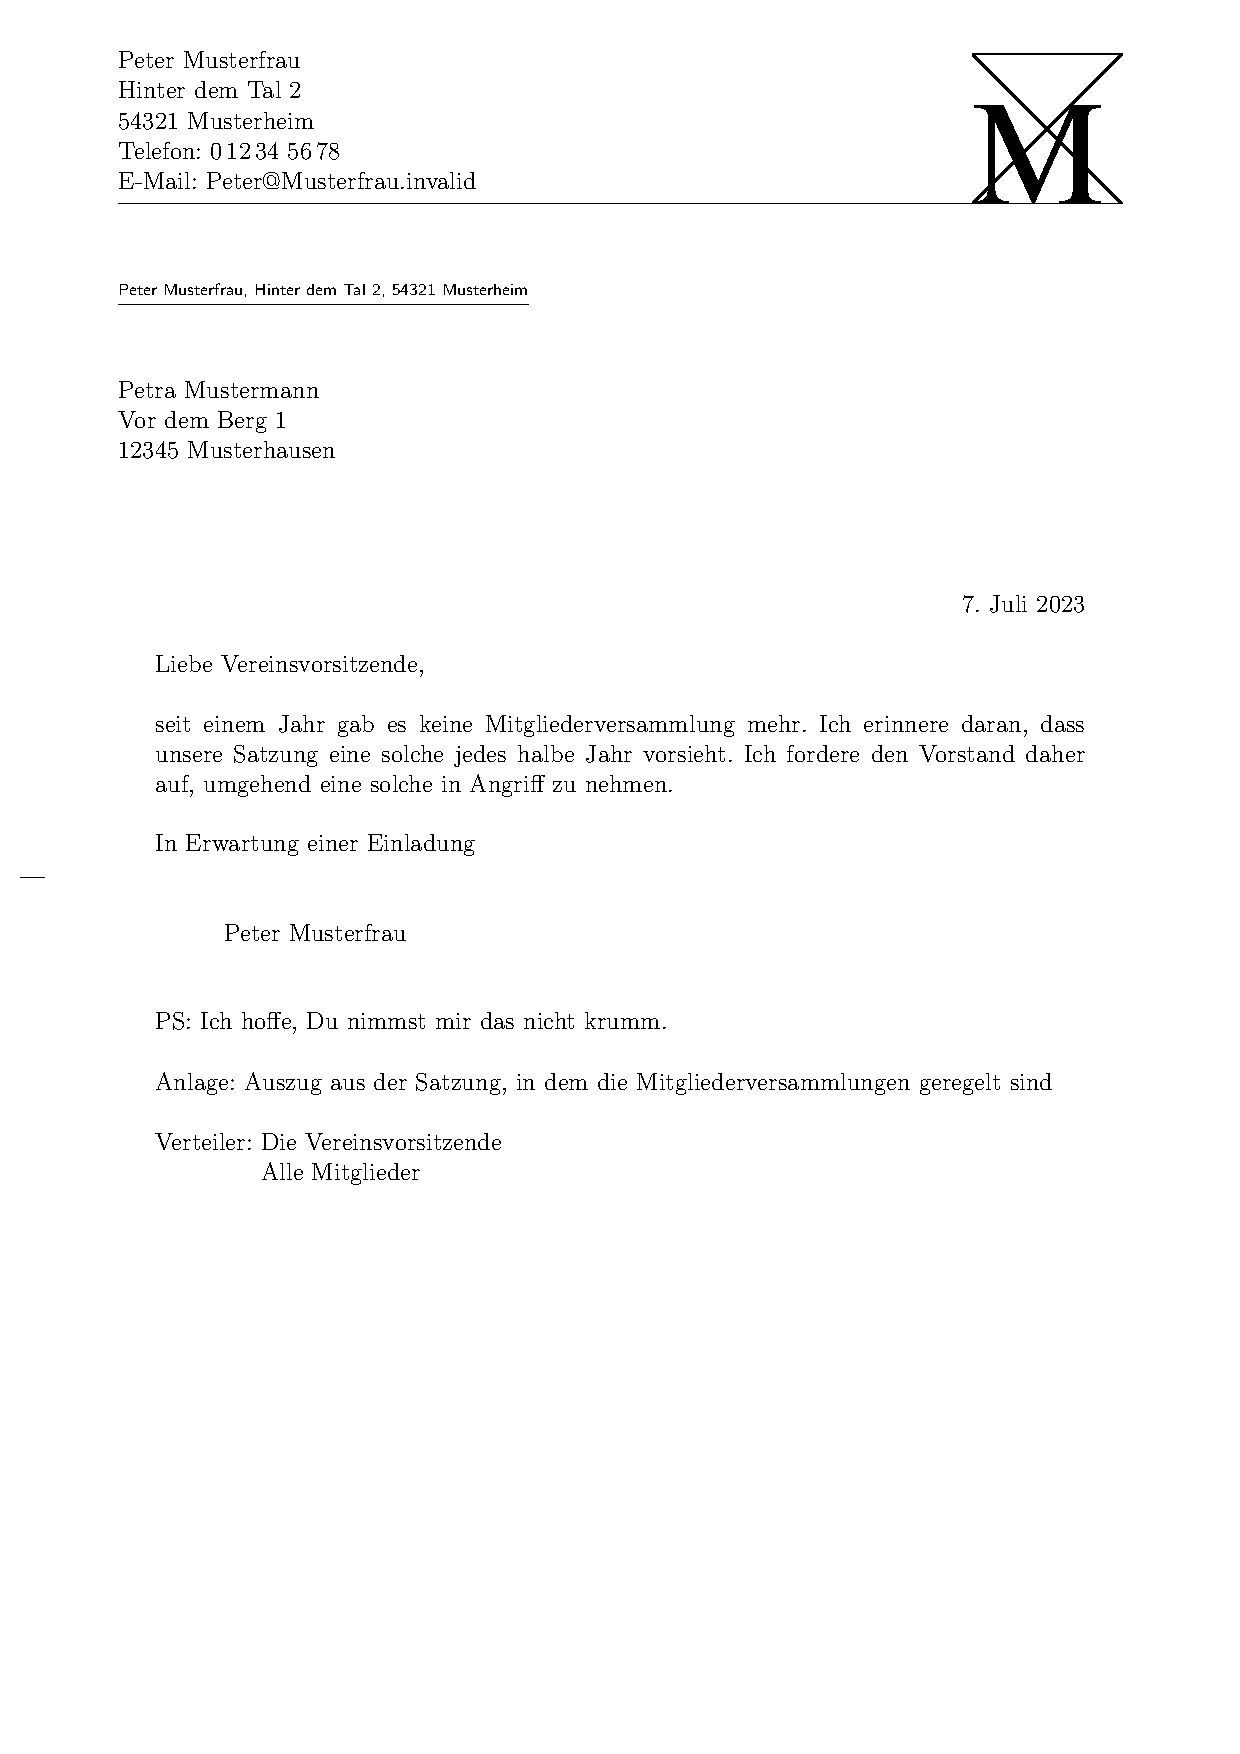
\includegraphics[width=.4\textwidth]{letter-example-16-de}}\quad
       \frame{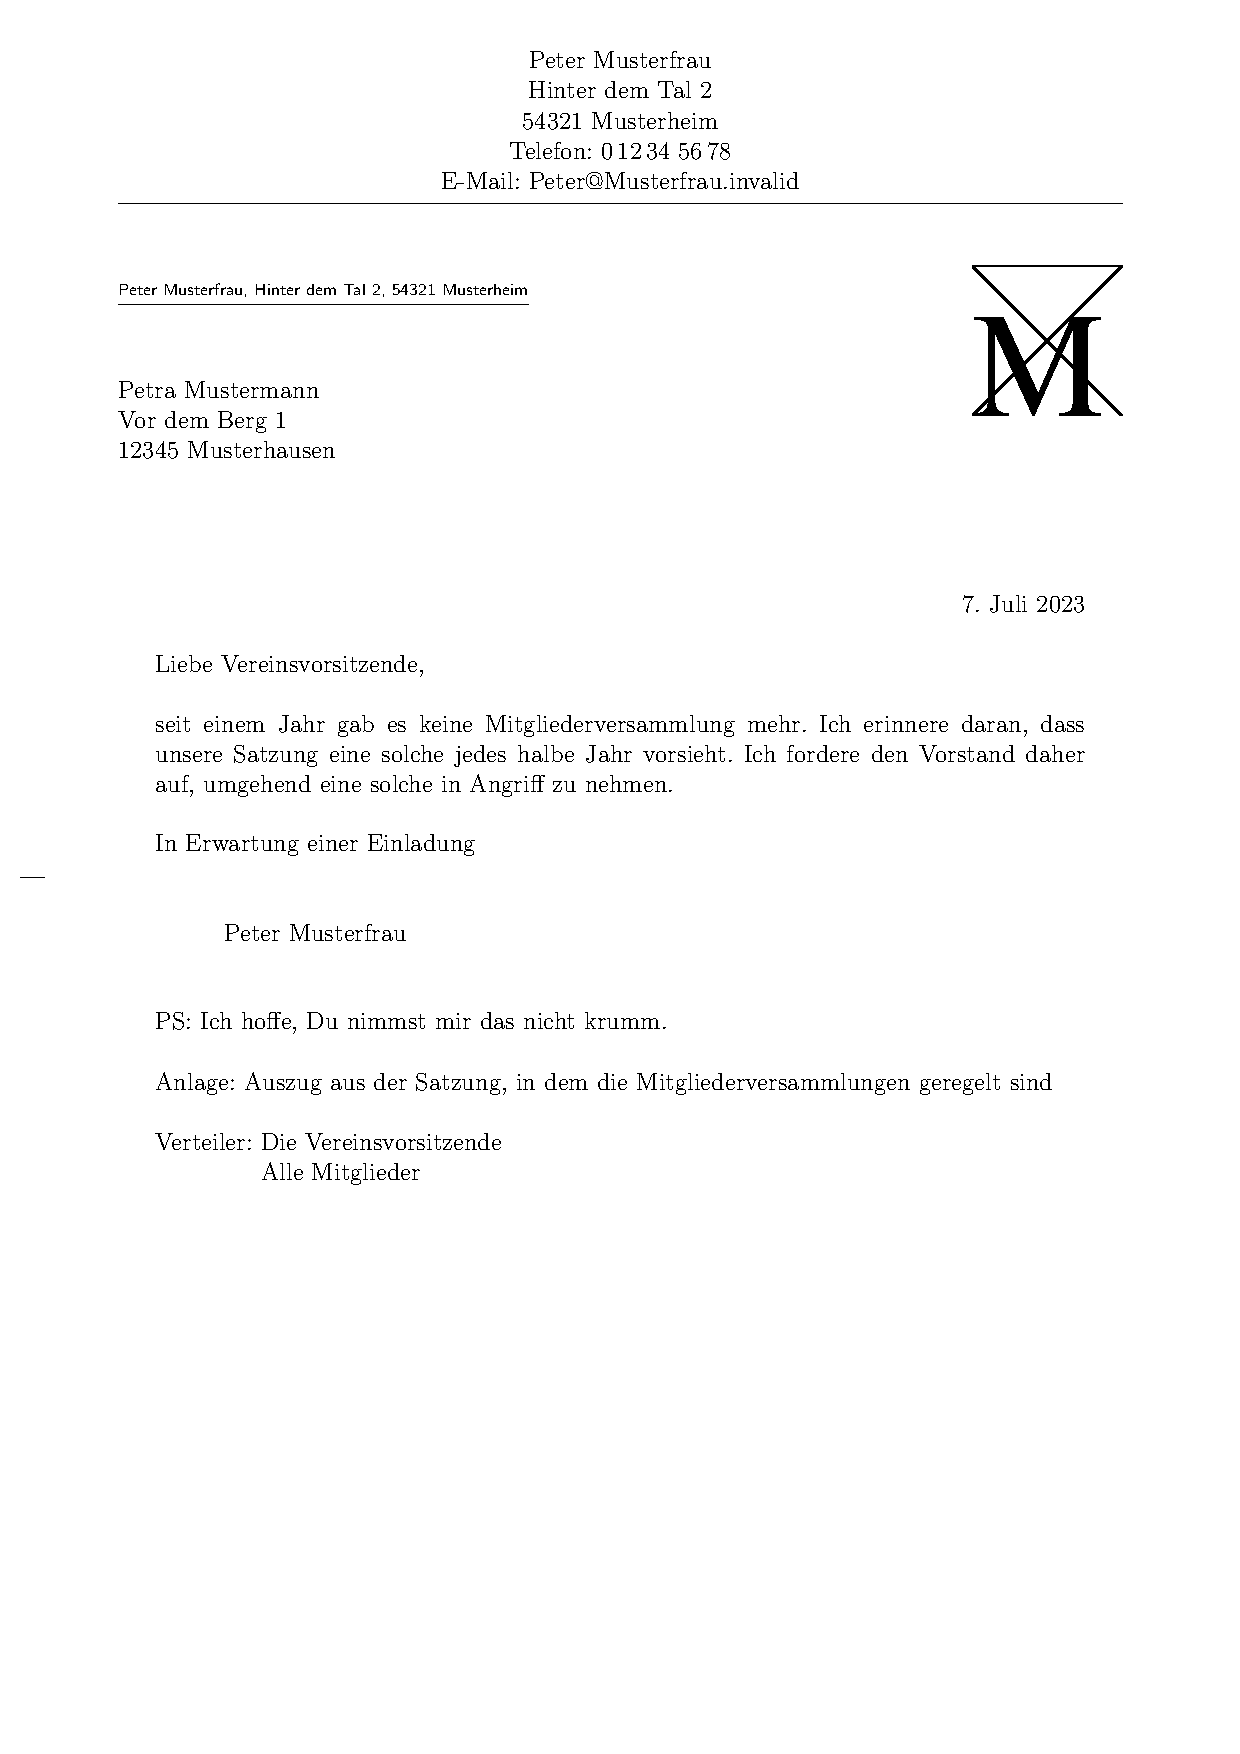
\includegraphics[width=.4\textwidth]{letter-example-17-de}}\par\bigskip}
     \begin{captionbeside}[{Beispiel: Brief mit erweitertem Absender, Logo,
         Trennlinie, Anschrift, Anrede, Text, Grußfloskel, Signatur,
         Postskriptum, Anlagen, Verteiler und Lochermarke; Absender links
         vs. rechts vs. zentriert}]{Ergebnis eines kleinen Briefes mit
         erweitertem Absender, Logo, Trennlinie, Anschrift, Anrede, Text,
         Grußfloskel, Signatur, Postskriptum, Anlagen, Verteiler und
         Lochermarke (das Datum entstammt den Voreinstellungen für
         DIN-Briefe); links, oben mit linksbündigem Absender, rechts daneben
         mit zentriertem Absender und rechts mit rechtsbündigem Absender}[l]
       \frame{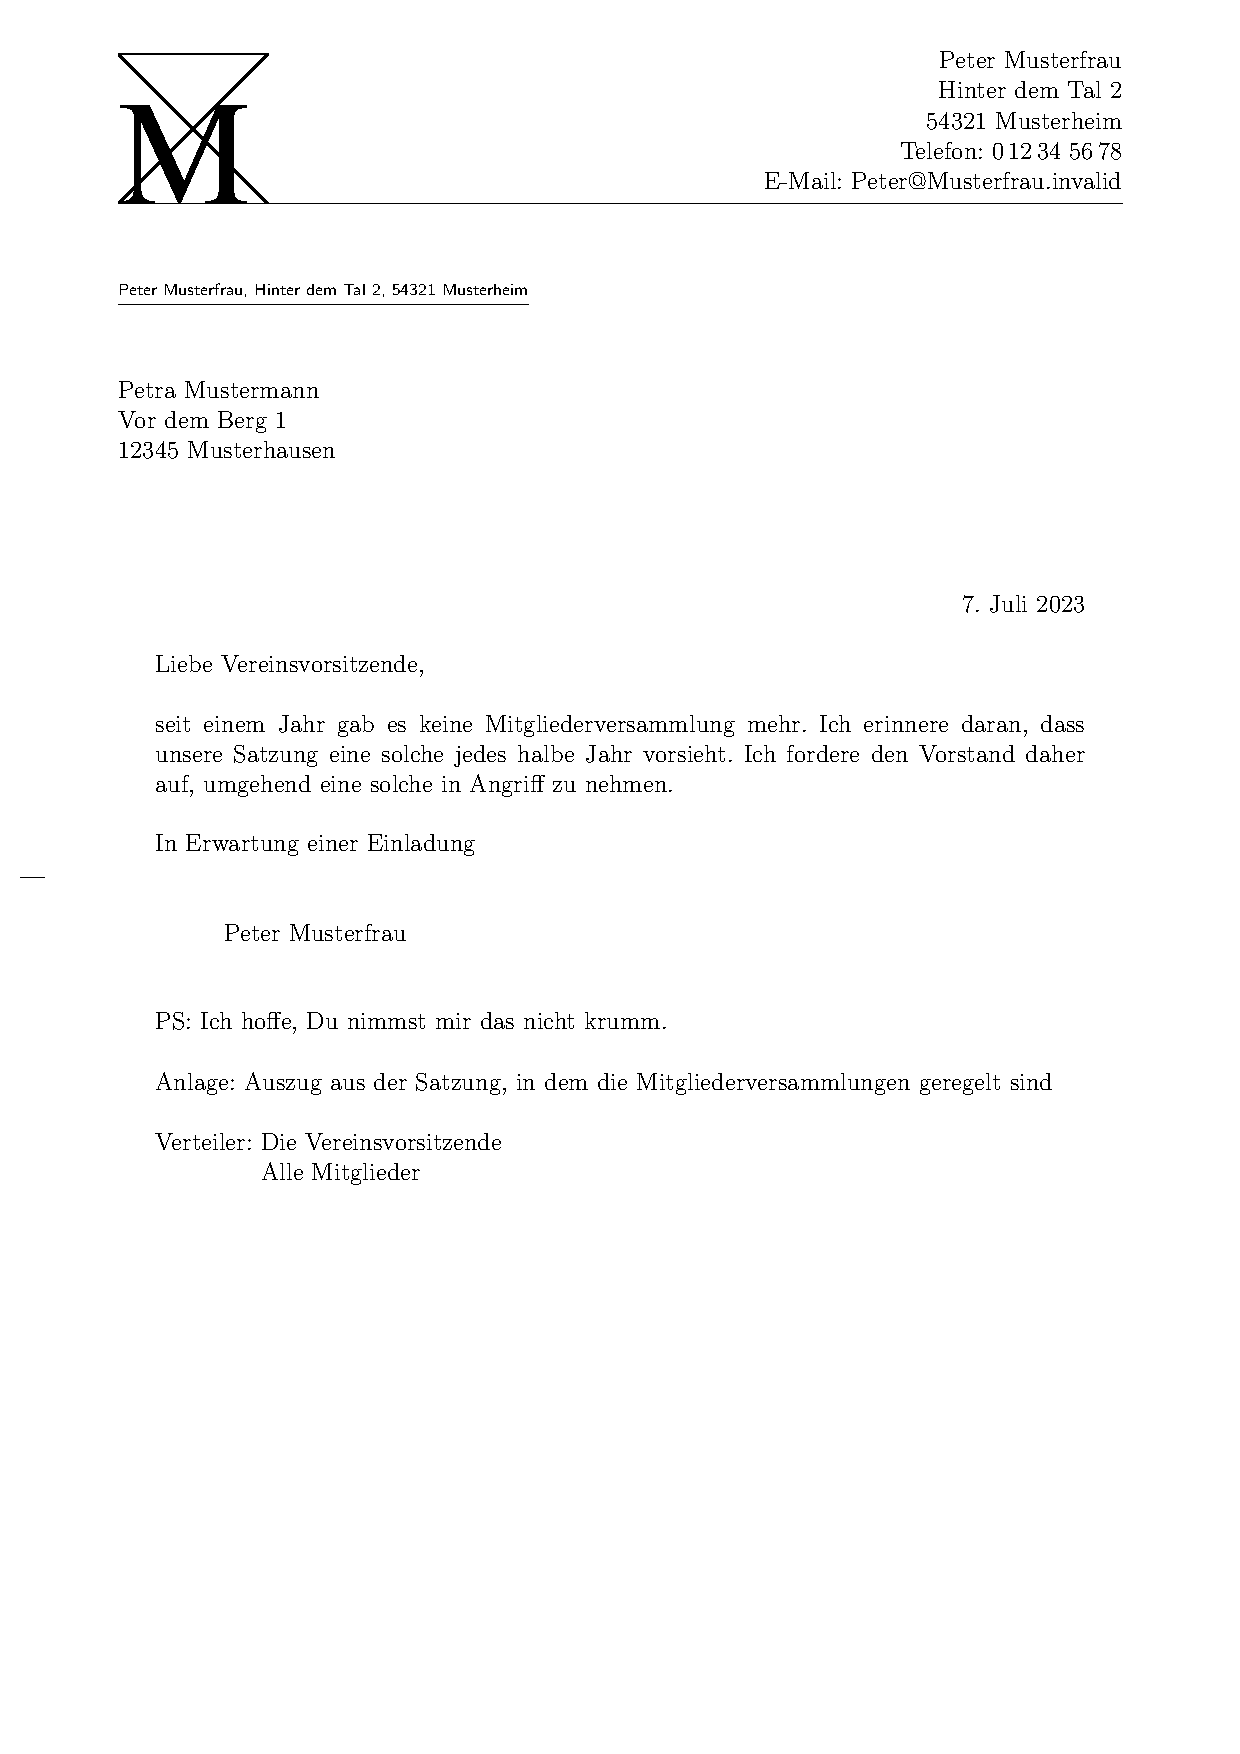
\includegraphics[width=.4\textwidth]{letter-example-18-de}}\quad
  \end{captionbeside}
  \label{fig:\LabelBase.letter-16-18}
  \end{figure}
\end{Example}%
%
\EndIndexGroup
\ExampleEndFix% Beispiel am Ende


\begin{Declaration}
  \Variable{firsthead}
\end{Declaration}
In vielen Fällen reichen die Möglichkeiten aus, die \Class{scrlttr2} über
Optionen und obige Variablen für die Gestaltung des Briefkopfes bietet. In
einigen Fällen will man jedoch den Briefkopf freier gestalten können. In
diesen Fällen muss man auf die Möglichkeiten der vordefinierten Briefköpfe,
die über die oben erwähnten Option ausgewählt werden können,
verzichten. Stattdessen gestaltet man sich seinen Briefkopf frei. Dazu
definiert man den gewünschten Aufbau über den \PName{Inhalt} der Variablen
\Variable{firsthead}. Dabei können beispielsweise mit Hilfe der
\Macro{parbox}-Anweisung (siehe \cite{latex:usrguide}) mehrere Boxen neben-
und untereinander gesetzt werden.  Einem versierten Anwender sollte es so
möglich sein, seinen eigenen Briefkopf zu gestalten. Natürlich kann und sollte
man dabei auch Zugriff auf andere Variablen mit Hilfe von
\DescRef{\LabelBase.cmd.usekomavar} nehmen. Die \PName{Bezeichnung} der
Variablen \Variable{firsthead} wird von \KOMAScript{} nicht verwendet.
\iffree{Ein ausführliches Beispiel für die Definition eines Briefkopfes ist
  beispielsweise im Anhang von \cite{book:komascript} und
  \cite{ebook:komascript} zu finden.%
}{Ein ausführliches Beispiel für die Definition eines Briefkopfes wird in
  \autoref{cha:modernletters} behandelt.}%
\EndIndexGroup
%
\EndIndexGroup


\subsection{Anschrift}
\seclabel{addressee}%
\BeginIndexGroup
\BeginIndex{}{Anschrift}%

% Verschiedene Umbruchvarianten
Unter der Anschrift versteht man normalerweise nur den Namen und die Adresse
des Empfängers. %
\iffalse%
Als \iffree{erste }{}Erweiterung zur Anschrift kann die
Versandart betrachtet werden, die etwa bei \iffree{Einschreiben oder
}{}Infobriefen zur Anwendung kommt. Bei Fensterbriefumschlägen wird auch die
sogenannte Rücksendeadresse \iffree{zur Anschrift}{dazu} gezählt, da sie im
Anschriftfenster zu sehen \iffree{sein wird}{ist}. Die Anschrift folgt
unmittelbar auf den Briefkopf.%
\else%
Aber auch die Versandart, beispielsweise bei Infobriefen, oder die
Rücksendeadresse werden als Teil des Anschriftfeldes gesetzt.%
\fi


\begin{Declaration}
  \OptionVName{addrfield}{Modus}
  \OptionVName{backaddress}{Wert}
  \OptionVName{priority}{Priorität}
  \Variable{toname}
  \Variable{toaddress}
  \Variable{backaddress}
  \Variable{backaddressseparator}
  \Variable{specialmail}
  \Variable{fromzipcode}
  \Variable{zipcodeseparator}
  \Variable{place}
  \Variable{PPcode}
  \Variable{PPdatamatrix}
  \Variable{addresseeimage}
\end{Declaration}%
\BeginIndex{}{Anschrift}%
Mit der Option \Option{addrfield} kann gewählt werden, ob ein Anschriftfeld
gesetzt werden soll oder nicht. Voreingestellt\textnote{Voreinstellung} ist
mit \PValue{true} die Verwendung eines Anschriftfeldes.  Die Option versteht
die in \autoref{tab:\LabelBase.addrfield}\ChangedAt{v3.03}{\Class{scrlttr2}}
%, \autopageref{tab:\LabelBase.addrfield} 
angegebenen Werte für den \PName{Modus}.  Bei den Werten \PValue{true},
\PValue{topaligned}\ChangedAt{v3.17}{\Class{scrlttr2}\and
  \Package{scrletter}}, \PValue{PP} und \PValue{backgroundimage} werden Name
und Adresse des Empfängers, die im Anschriftfeld gesetzt werden, über das
Argument der Umgebung \DescRef{\LabelBase.env.letter} (siehe
\autoref{sec:\LabelBase.document}, \DescPageRef{\LabelBase.env.letter})
bestimmt. Diese Angaben werden außerdem in die Variablen \Variable{toname} und
\Variable{toaddress} kopiert.

\BeginIndexGroup
\BeginIndex{FontElement}{addressee}\LabelFontElement{addressee}%
\BeginIndex{FontElement}{toname}\LabelFontElement{toname}%
\BeginIndex{FontElement}{toaddress}\LabelFontElement{toaddress}%
Die voreingestellten Schriftarten können\ChangedAt{v2.97c}{\Class{scrlttr2}}
über die Anweisungen \DescRef{\LabelBase.cmd.setkomafont} und
\DescRef{\LabelBase.cmd.addtokomafont} (siehe
\autoref{sec:\LabelBase.textmarkup}, ab
\DescPageRef{\LabelBase.cmd.setkomafont}) verändert werden. Dabei existieren
drei Elemente. Zunächst gibt es das Element
\FontElement{addressee}\IndexFontElement{addressee}%
\important{\FontElement{addressee}}, das generell für die Anschrift zuständig
ist. Dazu gibt es die Elemente
\FontElement{toname}\IndexFontElement{toname}\important{\FontElement{toname}}
und \FontElement{toaddress}\IndexFontElement{toaddress}%
\important{\FontElement{toaddress}}, die sich nur auf den Namen bzw. die
Adresse des Empfängers beziehen. Für \FontElement{toname} und
\FontElement{toaddress} können also Abweichungen von der Einstellung für
\FontElement{addressee} definiert werden.%
\EndIndexGroup
%
\begin{table}
  \caption[{Mögliche Werte für Option \Option{addrfield}}]%
  {Mögliche Werte für Option \Option{addrfield} zur
    Auswahl der Art der Anschrift%
    \label{tab:\LabelBase.addrfield}}%
  \begin{desctabular}
    \entry{\PValue{backgroundimage}, \PValue{PPbackgroundimage},
      \PValue{PPBackgroundImage}, \PValue{PPBackGroundImage},
      \PValue{ppbackgroundimage}, \PValue{ppBackgroundImage},
      \PValue{ppBackGroundImage}}{%
      Es wird eine Anschrift mit einer in Variable \Variable{addresseeimage}
      abgelegten Hintergrundgrafik als Port-Payé-Kopf (P.\,P.-Kopf), aber ohne
      Rücksendeadresse und Versandart gesetzt.}\\[-1.7ex]
    \entry{\PValue{false}, \PValue{off}, \PValue{no}}{%
      Es wird keine Anschrift gesetzt.}\\[-1.7ex]
    \entry{\PValue{image}, \PValue{Image}, \PValue{PPimage}, \PValue{PPImage},
      \PValue{ppimage}, \PValue{ppImage}}{%
      Eine in Variable \Variable{addresseeimage} abgelegte Abbildung wird als
      Anschrift mit Port-Payé gesetzt. Adressinformationen und Angaben für
      Rücksendeadresse, Versandart oder Priorität werden ignoriert.}\\[-1.7ex]
    \entry{\PValue{PP}, \PValue{pp}, \PValue{PPexplicite},
      \PValue{PPExplicite}, \PValue{ppexplicite}, \PValue{ppExplicite}}{%
      Es wird eine Anschrift mit explizit über die Variablen
      \Variable{fromzipcode}, \Variable{place} und \Variable{PPcode}
      ausgefülltem Port-Payé-Kopf (P.\,P.-Kopf), gegebenenfalls mit Priorität
      und über Variable \Variable{PPdatamatrix} gesetzter Data-Matrix, aber
      ohne Rücksendeadresse und Versandart gesetzt.}\\[-1.7ex]
    \entry{\PValue{topaligned}, \PValue{alignedtop}%
      \ChangedAt{v3.17}{\Class{scrlttr2}\and \Package{scrletter}}}{%
      Es wird eine Anschrift mit Rücksendeadresse und Versandart oder
      Priorität gesetzt. Die Anschrift wird dabei unter der Versandart nicht
      vertikal zentriert.}\\[-1.7ex]
    \entry{\PValue{true}, \PValue{on}, \PValue{yes}}{%
      Es wird eine Anschrift mit Rücksendeadresse und Versandart oder
      Priorität gesetzt.}%
  \end{desctabular}
\end{table}%

Im Anschriftfeld wird in der Voreinstellung \OptionValue{addrfield}{true}
zusätzlich noch die unterstrichene Rücksendeadresse gesetzt.  Mit Option
\Option{backaddress} kann gewählt werden, ob und in welcher Form die
Rücksendeadresse\Index{Ruecksendeadresse=Rücksendeadresse} für
Fensterbriefumschläge im Anschriftfeld gesetzt werden soll.  Die
Option\important{\OptionValue{backaddress}{false}} versteht dazu einerseits
die Standardwerte für einfache Schalter, die in \autoref{tab:truefalseswitch},
\autopageref{tab:truefalseswitch} angegeben sind. Dabei bleibt der Stil der
Rücksendeadresse unverändert. Beim Einschalten der Rücksendeadresse kann
andererseits\ChangedAt{v2.96}{\Class{scrlttr2}} gleichzeitig auch der Stil der
Rücksendeadresse gewählt werden. So aktiviert der Wert
\PValue{underlined}\important{\OptionValue{backaddress}{underlined}} die
unterstrichene Rücksendeadresse, während
\PValue{plain}\important{\OptionValue{backaddress}{plain}} den Stil ohne
Unterstreichung auswählt. Voreingestellt\textnote{Voreinstellung} ist
\PValue{underlined}, also das Setzen der unterstrichenen Rücksendeadresse.

Die Rücksendeadresse selbst wird über den \PName{Inhalt} der Variable
\Variable{backaddress} bestimmt. Voreingestellt ist hier der über
\DescRef{\LabelBase.variable.fromname} angegebene Name und die über
\DescRef{\LabelBase.variable.fromaddress} angegebene Adresse, wobei der
Doppelbackslash in diesem Fall durch den Inhalt der Variablen
\Variable{backaddressseparator} ersetzt wird. Für diese ist ein Komma, gefolgt
von einem nicht umbrechbaren Leerzeichen vordefiniert. Die \PName{Bezeichnung}
der Variablen \Variable{backaddress} wird von \KOMAScript{} nicht genutzt.
\BeginIndexGroup\BeginIndex{FontElement}{backaddress}%
\LabelFontElement{backaddress}%
Die Schriftart der Rücksendeadresse ist über das Element
\FontElement{backaddress}\important{\FontElement{backaddress}}
konfigurierbar. Voreingestellt ist hierbei
\ChangedAt{v3.39}{\Class{scrlttr2}}%
\DescRef{\LabelBase.cmd.maybesffamily}\IndexCmd{maybesffamily} (siehe
\autoref{tab:\LabelBase.AddresseeElements}). Vor der Anwendung der
konfigurierten Schriftumschaltung wird noch \Macro{scriptsize} ausgeführt.%
\EndIndexGroup

Während die Adresse in der Voreinstellung
\OptionValue{addrfield}{true}\ChangedAt{v3.17}{\Class{scrlttr2}\and
  \Package{scrletter}} im für die Anschrift verfügbaren Platz vertikal
zentriert wird, entfällt die Zentrierung mit
\OptionValue{addrfield}{topaligned}%
\important{\OptionValue{addrfield}{topaligned}}. Sie wird dann oben bündig im
verfügbaren Platz gesetzt.

\begin{table}
%  \centering
  \KOMAoptions{captions=topbeside}%
  \setcapindent{0pt}%
%  \caption
  \begin{captionbeside}[{%
      Schriftvoreinstellungen für die Elemente des Anschriftfensters%
    }]{%
      \hspace{0pt plus 1ex}%
      Voreinstellungen für die Schrift der Elemente des Anschriftfensters%
      \label{tab:\LabelBase.AddresseeElements}%
    }%
    [l]
  \begin{tabular}[t]{ll}
    \toprule
    Element & Voreinstellung \\
    \midrule
    \DescRef{\LabelBase.fontelement.addressee}\IndexFontElement{addressee} & 
    \\
    \ChangedAt{v3.39}{\Class{scrlttr2}}%
    \DescRef{\LabelBase.fontelement.backaddress}\IndexFontElement{backaddress} & 
    \DescRef{\LabelBase.cmd.maybesffamily}\IndexCmd{maybesffamily}%
    \\
    \DescRef{\LabelBase.fontelement.PPdata}\IndexFontElement{PPdata} &
    \Macro{sffamily}%
    \\
    \DescRef{\LabelBase.fontelement.PPlogo}\IndexFontElement{PPlogo} &
    \Macro{sffamily}\Macro{bfseries}%
    \\
    \DescRef{\LabelBase.fontelement.priority}\IndexFontElement{priority} &
    \Macro{fontsize}\PParameter{10pt}\PParameter{10pt}%
    \Macro{sffamily}\Macro{bfseries}%
    \\
    \DescRef{\LabelBase.fontelement.prioritykey}\IndexFontElement{prioritykey} &
    \Macro{fontsize}\PParameter{24.88pt}\PParameter{24.88pt}%
    \Macro{selectfont}%
    \\
    \DescRef{\LabelBase.fontelement.specialmail}\IndexFontElement{specialmail} & 
    \\
    \DescRef{\LabelBase.fontelement.toaddress}\IndexFontElement{toaddress} & 
    \\
    \DescRef{\LabelBase.fontelement.toname}\IndexFontElement{toname} & 
    \\
    \bottomrule
  \end{tabular}
  \end{captionbeside}
\end{table}

\BeginIndexGroup
\BeginIndex{FontElement}{specialmail}\LabelFontElement{specialmail} Zwischen
Rücksendeadresse und Empfängeradresse kann bei der Standardeinstellung
\OptionValue{addrfield}{true}\important{\OptionValue{addrfield}{true}} noch
eine optionale Versandart\Index{Versandart} gesetzt werden. Diese wird genau
dann gesetzt, wenn die Variable \Variable{specialmail} einen \PName{Inhalt}
hat und
\OptionValue{priority}{manual}\important{\OptionValue{priority}{manual}}%
\ChangedAt{v3.03}{\Class{scrlttr2}} gewählt wird, was der Voreinstellung
entspricht. Die \PName{Bezeichnung} von \Variable{specialmail} wird durch
\Class{scrlttr2} nicht genutzt. Die Ausrichtung wird mit Hilfe der
Pseudolängen \DescRef{\LabelBase.plength.specialmailindent} und
\DescRef{\LabelBase.plength.specialmailrightindent} (siehe
\DescPageRef{\LabelBase.plength.specialmailindent}) festgelegt. Die
voreingestellte Schriftart des Elements\ChangedAt{v2.97c}{\Class{scrlttr2}}
\FontElement{specialmail}\important{\FontElement{specialmail}}, die Sie
\autoref{tab:\LabelBase.AddresseeElements} entnehmen können, kann mit Hilfe
der Anweisungen \DescRef{\LabelBase.cmd.setkomafont} und
\DescRef{\LabelBase.cmd.addtokomafont} (siehe
\autoref{sec:\LabelBase.textmarkup}, \DescPageRef{\LabelBase.cmd.setkomafont})
verändert werden.%
\EndIndexGroup

\BeginIndexGroup
\BeginIndex{FontElement}{priority}\LabelFontElement{priority}%
\BeginIndex{FontElement}{prioritykey}\LabelFontElement{prioritykey}%
Wird\ChangedAt{v3.03}{\Class{scrlttr2}}%
\important[i]{\normalcolor\OptionValue{priority}{A}\\
  \normalcolor\OptionValue{priority}{B}} hingegen mit
\OptionValue{priority}{A} oder \OptionValue{priority}{B} (siehe
\autoref{tab:\LabelBase.priority}) eine internationale Priorität ausgewählt,
so wird diese bei \OptionValue{addrfield}{true} als Versandart und bei
\OptionValue{addrfield}{PP} an entsprechender Stelle im Port-Payé-Kopf
gesetzt. Dabei wird die
Grundschrift\important{\FontElement{priority}\\
  \FontElement{prioritykey}} über das Element \FontElement{priority} und die
davon abweichende Schrift für den Prioritätsschlüssel, »A« oder »B«, über das
Element \FontElement{prioritykey} bestimmt. Die voreingestellten Schriftarten
der beiden Elemente, die Sie \autoref{tab:\LabelBase.AddresseeElements}
entnehmen können, lassen sich mit den Anweisungen
\DescRef{\LabelBase.cmd.setkomafont} und
\DescRef{\LabelBase.cmd.addtokomafont} (siehe
\autoref{sec:\LabelBase.textmarkup}, \DescPageRef{\LabelBase.cmd.setkomafont})
ändern.%
\EndIndexGroup

\begin{table}
  \caption[{Mögliche Werte für Option \Option{priority}}]
  {Mögliche Werte für Option \Option{priority} zur
    Auswahl einer internationalen Priorität im Adressfeld}
  \label{tab:\LabelBase.priority}
  \begin{desctabular}
    \entry{\PValue{false}, \PValue{off}, \PValue{no}, \PValue{manual}}{%
      Es wird keine Priorität gesetzt.}\\[-1.7ex]
    \entry{\PValue{B}, \PValue{b}, \PValue{economy}, \PValue{Economy},
      \PValue{ECONOMY}, \PValue{B-ECONOMY}, \PValue{B-Economy},
      \PValue{b-economy}}{%
      Es wird die internationale Priorität B-Economy gesetzt. Bei
      \OptionValue{addrfield}{true} erfolgt dies anstelle der
      Versandart.}\\[-1.7ex]
    \entry{\PValue{A}, \PValue{a}, \PValue{priority}, \PValue{Priority},
      \PValue{PRIORITY}, \PValue{A-PRIORITY}, \PValue{A-Priority},
      \PValue{a-priority}}{%
      Es wird die internationale Priorität A-Priority gesetzt. Bei
      \OptionValue{addrfield}{true} erfolgt dies anstelle der Versandart.}%
  \end{desctabular}
\end{table}

Bei\ChangedAt{v3.03}{\Class{scrlttr2}}\important{\OptionValue{addrfield}{PP}}
\OptionValue{addrfield}{PP} wird im Port-Payé-Kopf die Postleitzahl aus der
Variablen \Variable{fromzipcode} und der Ort aus der Variablen
\Variable{place} gesetzt. Dabei wird der Postleitzahl, also dem \PName{Inhalt}
von \Variable{fromzipcode}, die \PName{Bezeichnung} der Variablen
\Variable{fromzipcode}, gefolgt vom \PName{Inhalt} von
\Variable{zipcodeseparator} vorangestellt. Für diese
\PName{Bezeichnung}\textnote{Voreinstellung} hängt die Voreinstellung von der
verwendeten \File{lco}-Datei (siehe \autoref{sec:\LabelBase.lcoFile} ab
\autopageref{sec:\LabelBase.lcoFile}) ab. Für den \PName{Inhalt} von
\Variable{zipcodeseparator} ist hingegen %
\iffalse % Umbruchvarianten
ein kleiner Abstand, gefolgt von einem Streckenstrich, gefolgt von einem
kleinen Abstand (\Macro{,}\texttt{-{}-}\Macro{,}) %
\else%
»\Macro{,}\texttt{-{}-}\Macro{,}« %
\fi%
voreingestellt.

Darüber\ChangedAt{v3.03}{\Class{scrlttr2}} hinaus wird bei
\OptionValue{addrfield}{PP}\important{\OptionValue{addrfield}{PP}} im
Port-Payé-Kopf auch noch ein Code gesetzt, der den Absender eindeutig
identifiziert. Dieser ist in Variable \Variable{PPcode} abgelegt. Rechts von
der Anschrift kann zusätzlich eine Data-Matrix gesetzt werden, die in Variable
\Variable{PPdatamatrix} abgelegt ist.

\BeginIndexGroup
\BeginIndex{FontElement}{PPdata}\LabelFontElement{PPdata}
Postleitzahl\ChangedAt{v3.03}{\Class{scrlttr2}}, Ort und Code werden in der
Voreinstellung mit einer Schrift der Größe 8\,pt gesetzt. Dabei wird die
Schrift des Elements \FontElement{PPdata}%
\important{\FontElement{PPdata}} verwendet. Dessen Voreinstellung ist
\autoref{tab:\LabelBase.AddresseeElements} zu entnehmen und kann mit Hilfe der
Anweisungen \DescRef{\LabelBase.cmd.setkomafont} und
\DescRef{\LabelBase.cmd.addtokomafont} (siehe
\autoref{sec:\LabelBase.textmarkup}, \DescPageRef{\LabelBase.cmd.setkomafont})
verändert werden.%
\EndIndexGroup

\BeginIndexGroup
\BeginIndex{FontElement}{PPlogo}\LabelFontElement{PPlogo}
Für den Port-Payé-Schriftzug »P.P.« kommt dagegen die Schrift des Elements
\FontElement{PPlogo}\important{\FontElement{PPlogo}} zur Anwendung. Dessen
Voreinstellung ist ebenfalls Tabelle
\autoref{tab:\LabelBase.AddresseeElements} zu entnehmen.%
\EndIndexGroup

Bei\important{\OptionValue{addrfield}{backgroundimage}\\
  \OptionValue{addrfield}{image}} den beiden Einstellungen
\OptionValue{addrfield}{backgroundimage}\ChangedAt{v3.03}{\Class{scrlttr2}}
und \OptionValue{addrfield}{image} wird eine Abbildung in das Adressfenster
gesetzt. Diese ist im \PName{Inhalt} der Variablen \Variable{addresseeimage}
abgelegt. Die \PName{Bezeichnung} dieser Variablen wird von \KOMAScript{}
nicht genutzt. Während bei Einstellung \OptionValue{addrfield}{image} außer der
Abbildung nichts gesetzt wird, wird bei
\OptionValue{addrfield}{backgroundimage} zusätzlich noch die Anschrift aus dem
obligatorischen Argument der \DescRef{\LabelBase.env.letter}-Umgebung
ausgegeben.

Die Anordnung des Port-Payé-Kopfes wird ebenso wie die Anordnung der
Port-Payé-Anschrift über die Pseudolängen
\DescRef{\LabelBase.plength.toaddrindent} (siehe
\DescPageRef{\LabelBase.plength.toaddrindent}) sowie
\DescRef{\LabelBase.plength.PPheadwidth} und
\DescRef{\LabelBase.plength.PPheadheight} (siehe
\DescPageRef{\LabelBase.plength.PPheadheight}) bestimmt. Für die Anordnung der
Data-Matrix ist die Pseudolänge \DescRef{\LabelBase.plength.PPdatamatrixvskip}
(siehe \DescPageRef{\LabelBase.plength.PPdatamatrixvskip}) zuständig.

Es\textnote{Achtung!} wird an dieser Stelle ausdrücklich darauf hingewiesen,
dass \KOMAScript{} selbst keine externen Abbildungen setzen kann. %
\iffalse % Umbruchkorrektur
Verwenden Sie für solche Abbildungen beispielsweise das Paket
\Package{graphicx}\IndexPackage{graphicx} und dessen Anweisung
\Macro{includegraphics}.%
\else%
Sollen also über die Variablen \Variable{addresseeimage} oder
\Variable{PPdatamatrix} externe Abbildungen gesetzt werden, so ist
beispielsweise das Grafikpaket \Package{graphics}\IndexPackage{graphics} oder
\Package{graphicx}\IndexPackage{graphicx} zu laden und in den Variablen dessen
Anweisung \Macro{includegraphics} zu verwenden.%
\fi%
\EndIndexGroup


\begin{Declaration}
  \PLength{toaddrvpos}
  \PLength{toaddrhpos}
\end{Declaration}
Diese Pseudolängen geben den Abstand des Anschriftfensters eines
Fensterbriefumschlags vom oberen und vom linken Rand des Papiers an.  Sie
werden in den vordefinierten
\File{lco}-Dateien\textnote{\File{lco}-Datei}\Index{lco-Datei=\File{lco}-Datei}
unterschiedlich eingestellt.  Für \PLength{toaddrhpos} gilt außerdem eine
Besonderheit. Ist\textnote{Achtung!} der Wert \iffree{}{wie bei \Option{SN}
  oder \Option{NF} }negativ, so ist sein Betrag der Abstand des
Anschriftfeldes vom rechten Rand des Papiers. %
\iffree{%
  Sie\textnote{Beispiele!} finden dies beispielsweise bei \Option{SN} oder
  \Option{NF}. Am kleinsten ist der Wert \PLength{toaddrvpos} bei
  \Option{DINmtext}. Hier kann es schnell passieren, dass der Briefkopf in das
  Anschriftfenster ragt.%
}{%
  Große Briefköpfe\textnote{Achtung!} können bei kleinem \PLength{toaddrvpos},
  beispielsweise bei \Option{DINmtext}, bis in das Anschriftfeld ragen.%
} Ob das Anschriftfenster überhaupt gesetzt wird, hängt von der Option
\DescRef{\LabelBase.option.addrfield}\IndexOption{addrfield} ab (siehe
\DescPageRef{\LabelBase.option.addrfield}).%
\EndIndexGroup


\begin{Declaration}
  \PLength{toaddrheight}
\end{Declaration}
Diese Pseudolänge gibt die Höhe des Anschriftfeldes einschließlich der
Versandart an. Ob Name und Adresse des Empfängers unter Berücksichtigung der
Versandart im Anschriftfeld vertikal zentriert werden, hängt von Option
\DescRef{\LabelBase.option.addrfield}\IndexOption{addrfield} ab.%
\EndIndexGroup


\begin{Declaration}
  \PLength{toaddrwidth}
\end{Declaration}
Diese Pseudolänge gibt die Breite des Anschriftfensters an. Sie wird in den
vordefinierten
\File{lco}-Dateien\textnote{\File{lco}-Datei}\Index{lco-Datei=\File{lco}-Datei}
entsprechend der unterschiedlichen Normen unterschiedlich
eingestellt. Typische Werte liegen zwischen 70\Unit{mm} und 100\Unit{mm}.

\begin{Example}
  Angenommen, Sie haben das Problem, dass Ihr Drucker einen \iffree{sehr
    breiten }{}unbedruckbaren rechten \iffree{oder linken }{}Rand von
  15\Unit{mm} besitzt. Dadurch kann bei Option \Option{SN} der Briefkopf, die
  Absenderergänzung und die Anschrift nicht komplett gedruckt werden. Sie
  erstellen daher eine neue \iffree{\File{lco}-Datei mit folgendem Inhalt}{Datei
    \File{SNmmarg.lco}, die Sie anstelle von \Option{SN} verwenden}:
\begin{lstcode}
  \ProvidesFile{SNmmarg.lco}
               [2002/06/04 v0.1 my own lco]
  \LoadLetterOption{SN}
  \addtoplength{toaddrwidth}{%
    -\useplength{toaddrhpos}}
  \setplength{toaddrhpos}{-15mm}
  \addtoplength{toaddrwidth}{%
    \useplength{toaddrhpos}}
  \endinput
\end{lstcode}%
  \iffree{ Bis Sie sich einen Drucker mit kleineren Rändern zugelegt haben,
    verwenden Sie \Option{SNmmarg} anstelle von
    \Option{SN}.}{}% Umbruchoptimierung
\end{Example}
%
\EndIndexGroup
\ExampleEndFix


\begin{Declaration}
  \PLength{toaddrindent}
\end{Declaration}
Manchmal will man, dass die Anschrift nicht am linken Rand des
Anschriftfensters beginnt und bis zum rechten Rand des Fensters reicht,
sondern ein wenig eingezogen wird. Der Wert dieses Einzugs kann über die
Pseudolänge \PLength{toaddrindent} festgelegt
werden. Typischerweise\textnote{Voreinstellung} ist dieser Wert jedoch
0\Unit{pt}.

Bei\textnote{Achtung!} jeder der
Einstellungen\ChangedAt{v3.03}{\Class{scrlttr2}}
\OptionValueRef{scrlttr2}{addrfield}{PP}\important{%
  \OptionValueRef{scrlttr2}{addrfield}{PP}\\
  \OptionValueRef{scrlttr2}{addrfield}{image}\\
  \OptionValueRef{scrlttr2}{addrfield}{backgroundimage}
}\IndexOption{addrfield~=\textKValue{PP}},
\OptionValueRef{scrlttr2}{addrfield}{image}%
\IndexOption{addrfield~=\textKValue{image}} und
\OptionValueRef{scrlttr2}{addrfield}{backgroundimage}%
\IndexOption{addrfield~=\textKValue{backgroundimage}} (siehe
\DescPageRef{\LabelBase.option.addrfield}) wird beim Wert 0\Unit{pt}
stattdessen ein Einzug von 8\Unit{mm} verwendet. Soll hier tatsächlich kein
Einzug verwendet werden, so kann mit 1\Unit{sp} ein vernachlässigbar kleiner
Einzug gesetzt werden. Des Weiteren wird \PLength{toaddrindent} bei den
genannten Einstellungen für
\DescRef{\LabelBase.option.addrfield}\IndexOption{addrfield} auch für den
Abstand zum rechten Rand des Anschriftfensters verwendet.%
\EndIndexGroup


\begin{Declaration}
  \PLength{backaddrheight}
\end{Declaration}
Bei Fensterbriefumschlägen wird der Absender häufig in einer kleinen Schrift
einzeilig über der Empfängeradresse ausgegeben. Diese Absenderangabe nennt man
Rücksendeadresse\textnote{Rücksendeadresse}%
\Index{Ruecksendeadresse=Rücksendeadresse}, da sie \iffree{im Anschriftfenster
  sichtbar ist und }{}der Post bei unzustellbaren Briefen für die Rücksendung
an den Absender dient. In dieser Adresse muss daher auch nur die Information
enthalten sein, die zur Rücksendung notwendig ist.

Die Höhe, die innerhalb des Anschriftfensters für die Rücksendeadresse zur
Verfügung steht, ist in der Pseudolänge \PLength{backaddrheight} abgelegt. Der
Wert\textnote{Voreinstellung} wird in den vordefinierten \File{lco}-Dateien
typischerweise auf 5\Unit{mm} eingestellt.  Ob die Rücksendeadresse überhaupt
gesetzt wird, bestimmt der Anwender mit den Optionen
\DescRef{\LabelBase.option.addrfield}\IndexOption{addrfield} (siehe
\DescPageRef{\LabelBase.option.addrfield}) und
\DescRef{\LabelBase.option.backaddress} (siehe
\DescPageRef{\LabelBase.option.backaddress}).%
\iftrue% Umbruchkorrektur
\ Ein Abschalten der Rücksendeadresse ist beispielsweise sinnvoll, wenn gar
keine Fensterbriefumschläge verwendet werden.%
\fi%
\EndIndexGroup


\begin{Declaration}
  \PLength{specialmailindent}
  \PLength{specialmailrightindent}
\end{Declaration}
Zwischen Rücksendeadresse und Empfängeradresse kann noch eine optionale
Versandart\Index{Versandart} gesetzt werden\iffree{. Diese wird genau dann
  gesetzt}{}, wenn die Variable \DescRef{\LabelBase.variable.specialmail}
einen Inhalt hat. Die Ausrichtung wird mit Hilfe der Pseudolängen
\PLength{specialmailindent} und \PLength{specialmailrightindent}
festgelegt. Diese geben den linken und rechten Einzug der Zeile an. In den
vordefinierten\textnote{Voreinstellung} \File{lco}-Dateien ist
\PLength{specialmailindent} auf den dehnbaren Wert \Macro{fill} gesetzt,
während \PLength{specialmailrightindent} auf 1\Unit{em} eingestellt ist. Damit
wird die Versandart 1\Unit{em} vom rechten Rand des Anschriftfensters
gesetzt.%
\EndIndexGroup


\begin{Declaration}
  \PLength{PPheadheight}
  \PLength{PPheadwidth}
\end{Declaration}
Die Pseudolänge \PLength{PPheadheight} gibt bei den beiden
Einstellungen\ChangedAt{v3.03}{\Class{scrlttr2}}
\OptionValueRef{scrlttr2}{addrfield}{PP}\important{%
  \OptionValueRef{scrlttr2}{addrfield}{PP}\\
  \OptionValueRef{scrlttr2}{addrfield}{backgroundimage}}%
\IndexOption{addrfield~=\textKValue{PP}} und
\OptionValueRef{scrlttr2}{addrfield}{backgroundimage}%
\IndexOption{addrfield~=\textKValue{backgroundimage}} die Höhe an, die am
Anfang des Adressfeldes für den Port-Payé-Kopf reserviert wird. Die
Pseudolänge \PLength{PPheadwidth} wird nur bei
\OptionValueRef{scrlttr2}{addrfield}{PP} (siehe
\DescPageRef{\LabelBase.option.addrfield}) verwendet und gibt die Breite des
linken Feldes des Port-Payé-Kopf mit dem P.\,P.-Logo, der Postleitzahl und dem
Ort an. Die Breite des rechten Feldes mit dem Code für den Absender und der
Priorität ist durch die Restbreite bestimmt.

Den\textnote{Achtung!\\Voreinstellung} normalerweise voreingestellten Wert von
0\Unit{mm} für Pseudolänge \PLength{PPheadheight} ändert \KOMAScript{}
selbstständig in 20,74\Unit{pt}. Den normalerweise voreingestellten Wert von
0\Unit{mm} für \PLength{PPheadwidth} ändert \KOMAScript{} selbstständig in
42\Unit{mm}.%
%
\EndIndexGroup


\begin{Declaration}
  \PLength{PPdatamatrixvskip}
\end{Declaration}
Durch\ChangedAt{v3.03}{\Class{scrlttr2}} diese Pseudolänge wird der vertikale
Abstand zwischen dem Port-Payé-Kopf und der Data-Matrix bei
\OptionValueRef{scrlttr2}{addrfield}{PP}%
\important{\OptionValueRef{scrlttr2}{addrfield}{PP}}%
\IndexOption{addrfield~=\textKValue{PP}} (siehe
\DescPageRef{\LabelBase.option.addrfield})
festgelegt. Den\textnote{Achtung!\\Voreinstellung} normalerweise
voreingestellten Wert von 0\Unit{mm} ändert \KOMAScript{} selbstständig in
9\Unit{mm}. Die Data-Matrix wird rechtsbündig zum Port-Payé-Kopf gesetzt.%
\EndIndexGroup
%
\EndIndexGroup


\subsection{Absenderergänzung}
\seclabel{locationField}
\BeginIndexGroup
\BeginIndex{}{Absenderergaenzung=Absenderergänzung}%

\iffalse% Umbruchvarianten
Insbesondere bei Geschäftsbriefen reicht der Platz im Briefkopf und im
Seitenfuß oftmals nicht aus, um alle Angaben des Absenders unterzubringen. Für
die zusätzlichen Informationen kann der Platz neben der Anschrift
genutzt werden. In dieser Anleitung wird dieses Feld \emph{Absenderergänzung}
genannt.%
\else%
\iffalse%
Reicht der Raum in Briefkopf und Seitenfuß nicht aus, um alle Angaben zum
Absender unterzubringen, kann der Platz neben der Anschrift als
\emph{Absenderergänzung} genutzt werden.%
\else%
Der freie Platz neben der Anschrift kann für zusätzliche Angaben zum Absender
genutzt werden.%
\fi%
\fi

\begin{Declaration}
  \OptionVName{locfield}{Einstellung}
\end{Declaration}
\BeginIndex{}{Absenderergaenzung=Absenderergänzung}%
Der Inhalt der Absenderergänzung neben der Anschrift ist frei wählbar.
Je\important{%
  \OptionValueRef{\LabelBase}{fromalign}{locationleft}\\
  \OptionValueRef{\LabelBase}{fromalign}{center}\\
  \OptionValueRef{\LabelBase}{fromalign}{locationright}} nach Einstellung der
oben erklärten Option \DescRef{\LabelBase.option.fromalign} wird sie außerdem
für das Logo des Absenders oder den Absender selbst mitverwendet. Die Breite
dieses Feldes kann beispielsweise in einer \File{lco}-Datei (siehe
\autoref{sec:\LabelBase.lcoFile}) gesetzt werden. Wird dort die Breite 0
gesetzt, so kann über die Option \Option{locfield} zwischen zwei
unterschiedlichen Voreinstellungen für die Breite dieses Feldes gewählt
werden. Dies ist bei der Mehrzahl der \File{lco}-Dateien der Fall, die
\KOMAScript{} beiliegen. Siehe hierzu auch die Erklärungen zur Pseudolänge
\DescRef{\LabelBase.plength.locwidth},
\DescPageRef{\LabelBase.plength.locwidth}. Mögliche Werte für die Option
sind \autoref{tab:\LabelBase.locfield} zu
entnehmen. Voreingestellt\textnote{Voreinstellung} ist \PValue{narrow}.
%
\begin{table}
%  \caption
  \KOMAoptions{captions=topbeside}%
  \setcapindent{0pt}%
  \begin{captionbeside}
    [{Mögliche Werte für Option \Option{locfield}}]
    {Mögliche Werte für Option \Option{locfield} zur Wahl der Breite des
      Feldes für die Absenderergänzung (Erklärung im Text beachten!)%
      \label{tab:\LabelBase.locfield}}%
    [l]
    \begin{minipage}[t]{.58\linewidth}
      \begin{desctabular}[t]
        \pventry{narrow}{schmales Feld für die Absenderergänzung}%
        \pventry{wide}{breites Feld für die Absenderergänzung}%
      \end{desctabular}
    \end{minipage}
  \end{captionbeside}
\end{table}


\begin{Declaration}
  \Variable{location}
\end{Declaration}
Der Inhalt der Absenderergänzung, soweit er nicht durch Logo oder den Absender
selbst belegt ist, wird mit der Variablen \Variable{location} festgelegt. Für
den \PName{Inhalt} dieser Variablen dürfen auch Formatierungsanweisungen wie
\Macro{raggedright} verwendet werden. Die \PName{Bezeichnung} dieser Variablen
wird von \KOMAScript{} nicht genutzt.

\begin{Example}
  Herr Musterfrau möchte ein paar zusätzliche Informationen zu seiner
  Mitgliedschaft angeben. Er wählt dazu die Absenderergänzung:%
  \lstinputcode[xleftmargin=1em]{letter-example-19-de.tex}%
  Das entsprechende Feld neben der Anschrift wird dann wie in
  \autoref{fig:\LabelBase.letter-19} gesetzt.
  \begin{figure}
    \setcapindent{0pt}%
    \begin{captionbeside}[{Beispiel: Brief mit erweitertem Absender, Logo,
        Anschrift, Absenderergänzung, Anrede, Text, Grußfloskel,
        Signatur, Postskriptum, Anlagen, Verteiler und Lochermarke}]{Ergebnis
        eines kleinen Briefes mit erweitertem Absender, Logo, 
        Anschrift, Absenderergänzung, Anrede, Text, Grußfloskel, Signatur,
        Postskriptum, Anlagen, Verteiler und Lochermarke (das Datum entstammt
        den Voreinstellungen für DIN-Briefe)}[l]
      \frame{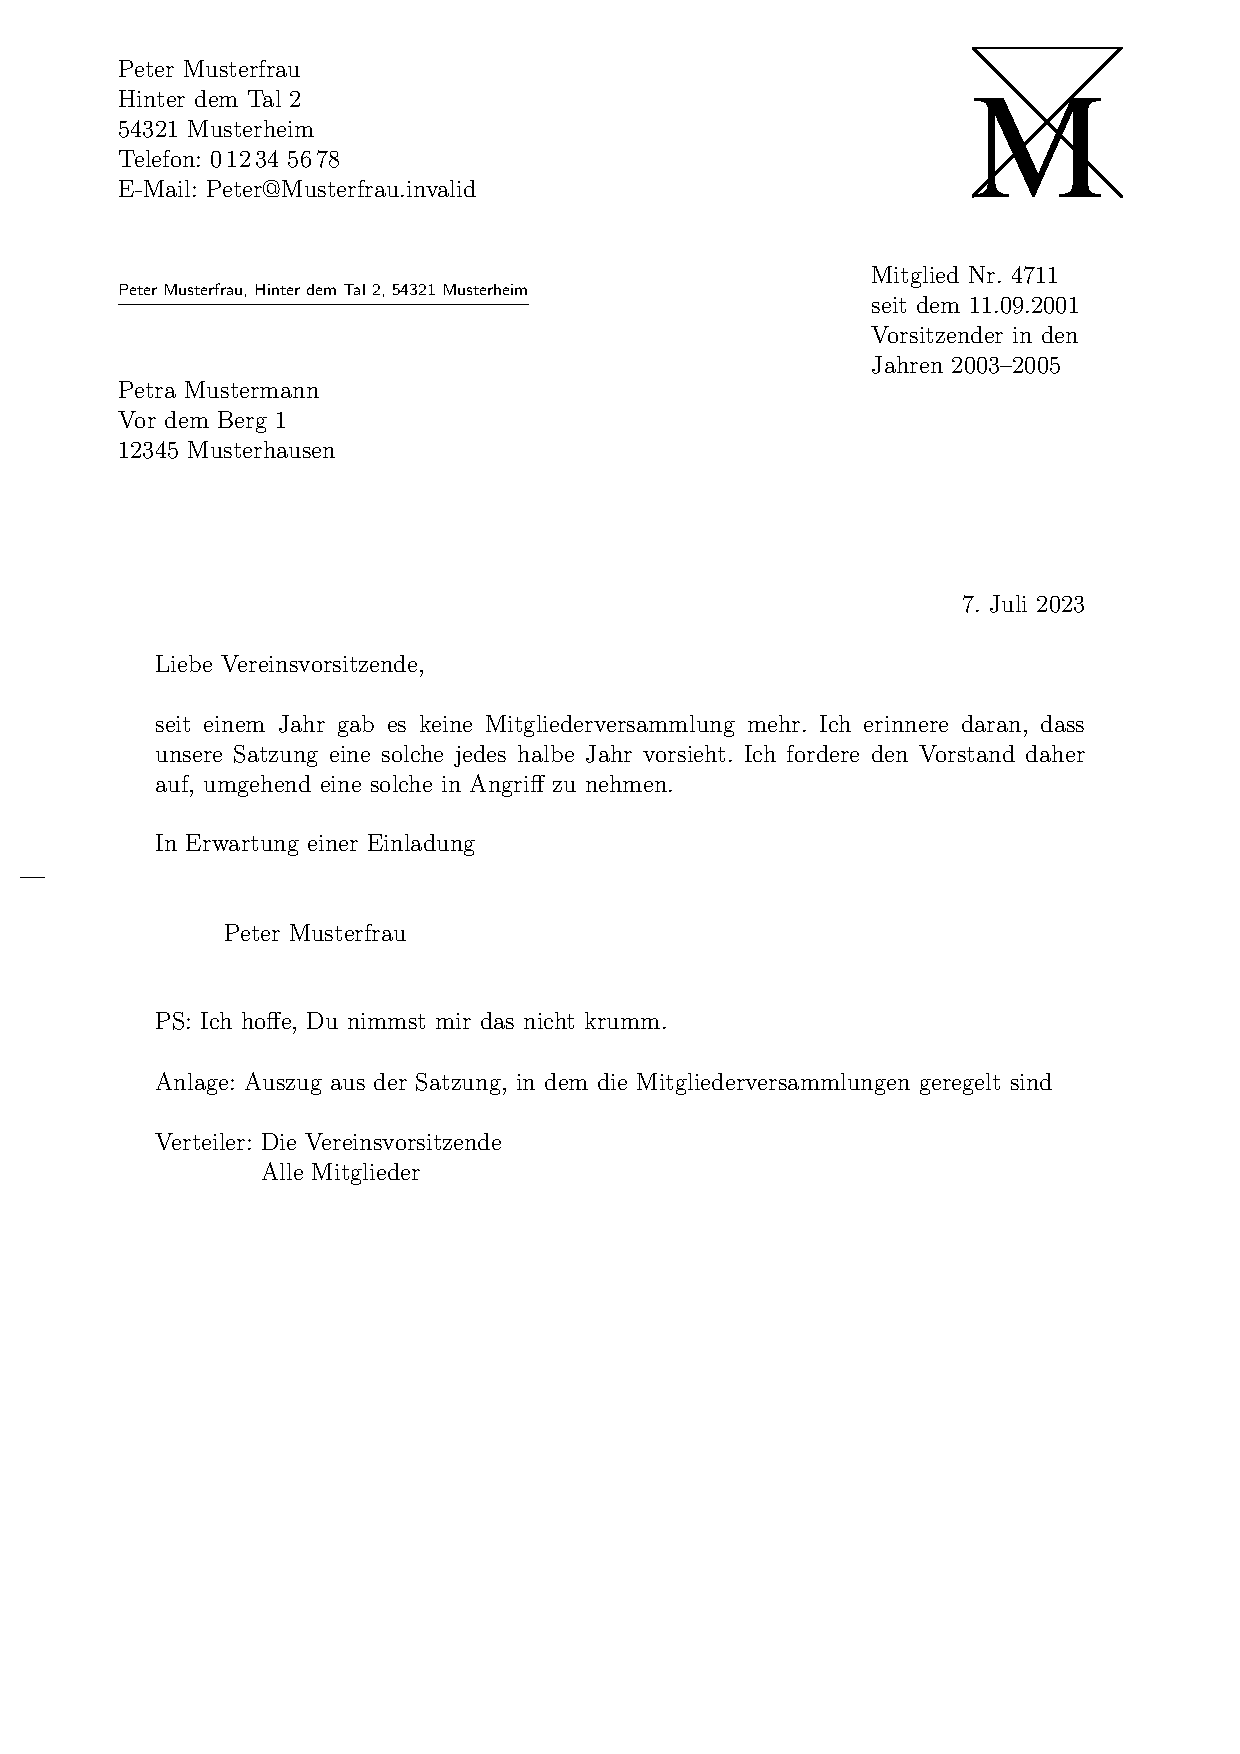
\includegraphics[width=.4\textwidth]{letter-example-19-de}}
    \end{captionbeside}
    \label{fig:\LabelBase.letter-19}
  \end{figure}
\end{Example}
%
\EndIndexGroup
\EndIndexGroup
\ExampleEndFix % Beispiel am Ende der Beschreibung


\begin{Declaration}
  \PLength{locheight}
  \PLength{lochpos}
  \PLength{locvpos}
  \PLength{locwidth}
\end{Declaration}
Die Pseudolängen \PLength{locwidth} und
\PLength{locheight}\ChangedAt{v2.97d}{\Class{scrlttr2}} geben die Breite und
Höhe der Absenderergänzung an. Die Pseudolängen \PLength{lochpos} und
\PLength{locvpos} geben die Abstände von der rechten, oberen
Papierecke an. Die Werte werden in den vordefinierten \File{lco}-Dateien
typischerweise auf 0\Unit{pt} gesetzt. Dieser\textnote{Achtung!} Wert nimmt
eine Sonderstellung ein. Er bedeutet, dass die Werte erst bei
\DescRef{\LabelBase.cmd.opening}\IndexCmd{opening} anhand der Breite des
Papiers, der Breite des Anschriftfensters, des Abstandes des
Anschriftfensters von der linken, oberen Papierecke und
Option \DescRef{\LabelBase.option.locfield} (siehe
\DescPageRef{\LabelBase.option.locfield})
gesetzt werden. Wie\textnote{Achtung!} bei \PLength{toaddrhpos} nehmen
negative Werte für \PLength{lochpos} eine Sonderstellung ein. Es wird dann
statt des Abstandes vom rechten Papierrand der Betrag von \PLength{lochpos}
als Abstand vom linken Papierrand verwendet. Die Bedeutung ist also genau
umgekehrt zu der bei \PLength{toaddrhpos} (siehe
\DescPageRef{\LabelBase.plength.toaddrhpos}).%
\EndIndexGroup
%
\EndIndexGroup


\subsection{Geschäftszeilen}
\seclabel{refLine}%
\BeginIndexGroup
\BeginIndex{}{Geschaeftszeile=Geschäftszeile}%

\iftrue % Umbruchkorrektur
Die Geschäftszeilen enthalten typischerweise Angaben wie Namenskürzel oder
Durchwahlnummern. \KOMAScript{} setzt automatisch nur nicht leere Felder. Ist
nur das Datum nicht leer, wird die Geschäftzeile zur Datumszeile.
\else%
Die Geschäftszeile kann auch länger als eine Zeile sein. Sie wird nur gesetzt,
wenn mindestens eine der Variablen für die Geschäftszeile nicht leer ist.  Es
werden nur nicht leere Felder gesetzt. Um\textnote{Tipp!} ein scheinbar leeres
Feld zu setzen, kann man einen scheinbar leeren Variableninhalt wie
\Macro{mbox}\Parameter{} verwenden. Wird auf die Geschäftszeile verzichtet, so
werden an ihrer Stelle Bezeichnung und Inhalt der Variablen
\DescRef{\LabelBase.variable.date} ausgegeben. %
\iffalse% Umbruchoptimierung
Informationen, wie Variablen zur Geschäftszeile hinzugefügt oder entfernt
werden, sind in \autoref{sec:scrlttr2-experts.variables},
\DescPageRef{scrlttr2-experts.cmd.removereffields} zu finden.%
\fi%
\fi

\begin{Declaration}
  \OptionVName{numericaldate}{Ein-Aus-Wert}
\end{Declaration}
Mit dieser Option kann zwischen der sprachabhängigen Standarddarstellung des
Datums\Index{Datum} in
\Macro{today}\IndexCmd[indexmain]{today}\important{\Macro{today}} und einem
ebenfalls sprachabhängigen rein numerischen Datum umgeschaltet werden. Die
Standarddarstellung wird nicht von \KOMAScript{} bereitgestellt. Sie kann
wahlweise vom \LaTeX-Kern oder einem Paket wie
\Package{babel}\IndexPackage{babel} oder
\Package{isodate}\IndexPackage{isodate}
stammen. Das\important{\OptionValue{numericaldate}{true}} kurze numerische
Datum wird hingegen von \Class{scrlttr2} selbst erzeugt. Die Option versteht
die Standardwerte für einfache Schalter, die in \autoref{tab:truefalseswitch},
\autopageref{tab:truefalseswitch} angegeben
sind. Voreingestellt\textnote{Voreinstellung} ist mit \PValue{false} die
Verwendung der Standarddarstellung.

\begin{Declaration}
  \Variable{date}
\end{Declaration}
Das Datum \iffalse % Umbruchkorektur (stimmt das so?)
in der gewählten Darstellung %
\fi %
wird im \PName{Inhalt} der Variablen \Variable{date}
abgelegt. Voreingestellt\textnote{Voreinstellung} ist das mit
\Macro{date}\IndexCmd{date} gesetzte Datum, das selbst mit
\Macro{today}\important{\Macro{date}, \Macro{today}}\IndexCmd{today}
voreingestellt ist. Damit ist der \PName{Inhalt} der Variablen nur indirekt
von Option \DescRef{\LabelBase.option.numericaldate}%
\important{\DescRef{\LabelBase.option.numericaldate}} abhängig.

Gesetzt wird das Datum normalerweise
als Teil der Geschäftszeile. Wenn die Geschäftszeile ansonsten leer bleibt,
wird allerdings nur eine Datumszeile, bestehend aus dem Ort und dem Datum,
gesetzt. Trotzdem haben auch in diesem Fall die Einstellungen der nachfolgend
beschriebenen Option \DescRef{\LabelBase.option.refline} Auswirkungen auf
diese Datumszeile. Weitere Informationen zum Ort finden Sie in der
Beschreibung zur Variablen
\DescRef{\LabelBase.variable.placeseparator}\IndexVariable{placeseparator} auf
\DescPageRef{\LabelBase.variable.placeseparator}.%
%
\EndIndexGroup
\EndIndexGroup


\begin{Declaration}
  \OptionVName{refline}{Einstellung}
\end{Declaration}
\BeginIndex{}{Geschaeftszeile=Geschäftszeile}%
\iffalse% Überflüssig
Insbesondere bei Geschäftsbriefen findet sich häufig eine Zeile mit Angaben
wie Namenskürzeln\Index{Kuerzel=Kürzel}, Durchwahl\Index{Durchwahl},
Kunden-\Index{Kundennummer} und Rechnungsnummer\Index{Rechnungsnummer} oder
zur Bezugnahme auf ein früheres Schreiben. Diese Zeile wird in dieser
Anleitung \emph{Geschäftszeile}\textnote{Geschäftszeile} genannt.

\fi%
Bei \Class{scrlttr2} und \Package{scrletter} können Kopf, Fuß, Anschrift und
das Feld mit der Absenderergänzung links und rechts aus dem normalen
Satzspiegel herausragen.  Über
\OptionValue{refline}{wide}\important{\OptionValue{refline}{wide}} kann
gewählt werden, dass dies auch für die Geschäftszeile gelten soll. %
\iffalse% Hier überflüssig
Die Geschäftszeile enthält normalerweise zumindest das Datum, kann aber auch
weitere Angaben aufnehmen. %
\fi%
Mögliche Werte für diese Option sind \autoref{tab:\LabelBase.refline} zu
entnehmen. Voreingestellt\textnote{Voreinstellung} sind \PValue{narrow} und
\PValue{dateright}\ChangedAt{v3.09}{\Class{scrlttr2}}.%
%
\begin{table}
  \caption[{Mögliche Werte für Option \Option{refline}}]
  {Mögliche Werte für Option \Option{refline} zur
    Konfiguration der Geschäftszeile}
  \label{tab:\LabelBase.refline}
  \begin{desctabular}
    \pventry{dateleft}{\ChangedAt{v3.09}{\Class{scrlttr2}}%
      Das Datum steht automatisch links in der Geschäftszeile.}%
    \pventry{dateright}{\ChangedAt{v3.09}{\Class{scrlttr2}}%
      Das Datum steht automatisch rechts in der Geschäftszeile.}%
    \pventry{narrow}{Die Breite der Geschäftszeile richtet sich nach dem
      Satzspiegel.}%
    \pventry{nodate}{\ChangedAt{v3.09}{\Class{scrlttr2}}%
      Das Datum wird nicht automatisch in die Geschäftszeile gesetzt.}%
    \pventry{wide}{Die Breite der Geschäftszeile richtet sich nach Anschrift
      und Absenderergänzung.}%
  \end{desctabular}
\end{table}


\begin{Declaration}
  \Variable{yourref}
  \Variable{yourmail}
  \Variable{myref}
  \Variable{customer}
  \Variable{invoice}
\end{Declaration}
Typische Felder der Geschäftszeile werden über die fünf Variablen
\Variable{yourref}, \Variable{yourmail}, \Variable{myref}, \Variable{customer}
und \Variable{invoice} verwaltet. %
\iffalse % Umbruchkorrektur
Die Bedeutung dieser Felder %
\else %
Ihre Bedeutung %
\fi %
ist \autoref{tab:\LabelBase.variables}, \autopageref{tab:\LabelBase.variables}
zu entnehmen. Jede dieser Variablen hat auch eine vordefinierte
\PName{Bezeichnung}, die in \autoref{tab:\LabelBase.reflineTerm} zu finden
ist. Wie weitere Variablen zur Geschäftszeile hinzugefügt werden können, ist
in \autoref{sec:scrlttr2-experts.variables} ab
\DescPageRef{scrlttr2-experts.cmd.newkomavar} erklärt.

\begin{table}
%  \centering
  \KOMAoptions{captions=topbeside}%
  \setcapindent{0pt}%
%  \caption
  \begin{captionbeside}
    [{Vordefinierte Bezeichnungen der Variablen der
      Geschäftszeile}]
    {Vordefinierte Bezeichnungen der typischen Variablen der
      Geschäftszeile unter Verwendung sprachabhängiger Anweisungen%
      \label{tab:\LabelBase.reflineTerm}%
    }
    [l]
    \begin{tabular}[t]{lll}
      \toprule
      Name                & Bezeichnung  & bei deutscher Sprache \\
      \midrule
      \Variable{yourref}  & \DescRef{scrlttr2-experts.cmd.yourrefname}  & Ihr Zeichen \\
      \Variable{yourmail} & \DescRef{scrlttr2-experts.cmd.yourmailname} & Ihr Schreiben vom \\
      \Variable{myref}    & \DescRef{scrlttr2-experts.cmd.myrefname}    & Unser Zeichen \\
      \Variable{customer} & \DescRef{scrlttr2-experts.cmd.customername} & Kundennummer \\
      \Variable{invoice}  & \DescRef{scrlttr2-experts.cmd.invoicename}  & Rechnungsnummer \\
      \DescRef{\LabelBase.variable.date}     & \DescRef{scrlttr2-experts.cmd.datename}     & Datum \\
      \bottomrule
    \end{tabular}
  \end{captionbeside}
\end{table}

\BeginIndexGroup
\BeginIndex{FontElement}{refname}\LabelFontElement{refname}%
\BeginIndex{FontElement}{refvalue}\LabelFontElement{refvalue}%
Schriftart und Farbe\ChangedAt{v2.97c}{\Class{scrlttr2}} der Feldbezeichnung
und des Feldinhalts können über die beiden Elemente
\FontElement{refname}\important{\FontElement{refname}, \FontElement{refvalue}}
und \FontElement{refvalue} geändert werden. Dazu werden die Anweisungen
\DescRef{\LabelBase.cmd.setkomafont} und
\DescRef{\LabelBase.cmd.addtokomafont} (siehe
\autoref{sec:\LabelBase.textmarkup}, \DescPageRef{\LabelBase.cmd.setkomafont})
verwendet. Die Voreinstellungen der \iffree{beiden }{}Elemente sind
\autoref{tab:\LabelBase.refnamerefvalue} zu entnehmen.%
\begin{table}[tp]
%  \centering
  \KOMAoptions{captions=topbeside}%
  \setcapindent{0pt}%
%  \caption
  \begin{captionbeside}
    [{Schriftvoreinstellungen für die Elemente der Geschäftszeile}]
    {Voreinstellungen für die Schrift der Elemente der Geschäftszeile%
      \label{tab:\LabelBase.refnamerefvalue}}
    [l]
    \begin{tabular}[t]{ll}
      \toprule
      Element & Voreinstellung \\
      \midrule
      \ChangedAt{v3.39}{\Class{scrlttr2}}%
      \FontElement{refname}
              & \DescRef{\LabelBase.cmd.maybesffamily}\IndexCmd{maybesffamily}%
                \Macro{scriptsize} \\
      \FontElement{refvalue} & \\
      \bottomrule
    \end{tabular}
  \end{captionbeside}
\end{table}%
%
\EndIndexGroup


\begin{Declaration}
  \Variable{placeseparator}
\end{Declaration}%
Sind bis auf \DescRef{\LabelBase.variable.date}%
\important{\DescRef{\LabelBase.variable.date}}\IndexVariable{date} alle
Variablen der Geschäftszeile leer, so wird keine echte Geschäftszeile
gesetzt. Stattdessen\textnote{Datumszeile} werden dann nur Ort\Index{Ort} und
Datum\Index{Datum} ausgegeben. Dabei bestimmt der \PName{Inhalt} der Variablen
\DescRef{\LabelBase.variable.place}\IndexVariable{place}%
\important{\DescRef{\LabelBase.variable.place}} den Ort. Für das Trennzeichen,
das in diesem Fall nach dem Ort gesetzt wird, ist der \PName{Inhalt} der
Variablen \Variable{placeseparator} zuständig. Der
vordefinierte\textnote{Voreinstellung} \PName{Inhalt} des Trennzeichens ist
dabei ein Komma, gefolgt von einem nicht umbrechbaren Leerzeichen. Ist der Ort
leer, so wird auch das Trennzeichen nicht gesetzt.%
\iffalse % Umbruchkorrektur
\ Der vordefinierte \PName{Inhalt} der Variablen
\DescRef{\LabelBase.variable.date} ist
\Macro{today}\IndexCmd{today}\important{\Macro{today}} und hängt indirekt von
der Einstellung der Option \DescRef{\LabelBase.option.numericaldate}%
\important{\DescRef{\LabelBase.option.numericaldate}}%
\IndexOption{numericaldate} ab (siehe
\DescPageRef{\LabelBase.option.numericaldate}).%
\fi %

\BeginIndexGroup
\BeginIndex{FontElement}{placeanddate}\LabelFontElement{placeanddate}%
Für\ChangedAt{v3.12}{\Class{scrlttr2}} eine solche Datumszeile mit Ort findet
nicht die Schrifteinstellung des Elements
\DescRef{\LabelBase.fontelement.refvalue} Anwendung. Stattdessen wird das
Element \FontElement{placeanddate}\important{\FontElement{placeanddate}}
verwendet, dessen leere Voreinstellung mit Hilfe der Anweisungen
\DescRef{\LabelBase.cmd.setkomafont} und
\DescRef{\LabelBase.cmd.addtokomafont} (siehe
\autoref{sec:\LabelBase.textmarkup}, \DescPageRef{\LabelBase.cmd.setkomafont})
geändert werden kann.%
\EndIndexGroup

\iffalse% Umbruchkorrektur
Seit Version~3.09\ChangedAt{v3.09}{\Class{scrlttr2}} werden Ort und Datum
nicht mehr zwingend rechtsbündig ausgegeben. Stattdessen findet auch im Falle
der Datumszeile die Datumseinstellung von Option
\DescRef{\LabelBase.option.refline}\IndexOption{refline}%
\important{\DescRef{\LabelBase.option.refline}}, wie sie in
\autoref{tab:\LabelBase.refline} angegeben ist, Anwendung.%
\else%
Die in \autoref{tab:\LabelBase.refline} angegebenen Datumseinstellungen
\iffree{für \DescRef{\LabelBase.option.refline}\IndexOption{refline}%
  \important{\DescRef{\LabelBase.option.refline}} }{}% Umbruchkorrektur
werden auch von der Datumszeile
beachtet. Voreingestellt\textnote{Voreinstellung} ist rechtsbündig.%
\fi

\begin{Example}
  Herr Musterfrau setzt nun auch die Variable für den Ort:
  \lstinputcode[xleftmargin=1em]{letter-example-20-de.tex}%
  \iffalse% Umbruchkorrektur
  Damit erscheint vor dem Datum, wie in \autoref{fig:\LabelBase.letter-20} zu
  sehen, %
  \else%
  In \autoref{fig:\LabelBase.letter-20} erscheint damit %
  \fi %
  der Ort, gefolgt von den automatischen Trennzeichen vor dem Datum. Dieses
  Datum wurde im Beispielcode über Variable \DescRef{\LabelBase.variable.date}
  explizit gesetzt, damit bei einem späteren \LaTeX-Durchlauf des Briefes das
  ursprüngliche Datum erhalten bleibt und nicht automatisch das Datum des
  \LaTeX-Laufs verwendet wird.
  \begin{figure}
    \setcapindent{0pt}%
    \begin{captionbeside}[{Beispiel: Brief mit erweitertem Absender, Logo,
        Anschrift, Absenderergänzung, Ort, Datum, Anrede, Text,
        Grußfloskel, Signatur, Postskriptum, Anlagen, Verteiler und
        Lochermarke}]{Ergebnis eines kleinen Briefes mit erweitertem Absender,
        Logo, Anschrift, Absenderergänzung, Ort, Datum, Anrede,
        Text, Grußfloskel, Signatur, Postskriptum, Anlagen, Verteiler und
        Lochermarke}[l]
      \frame{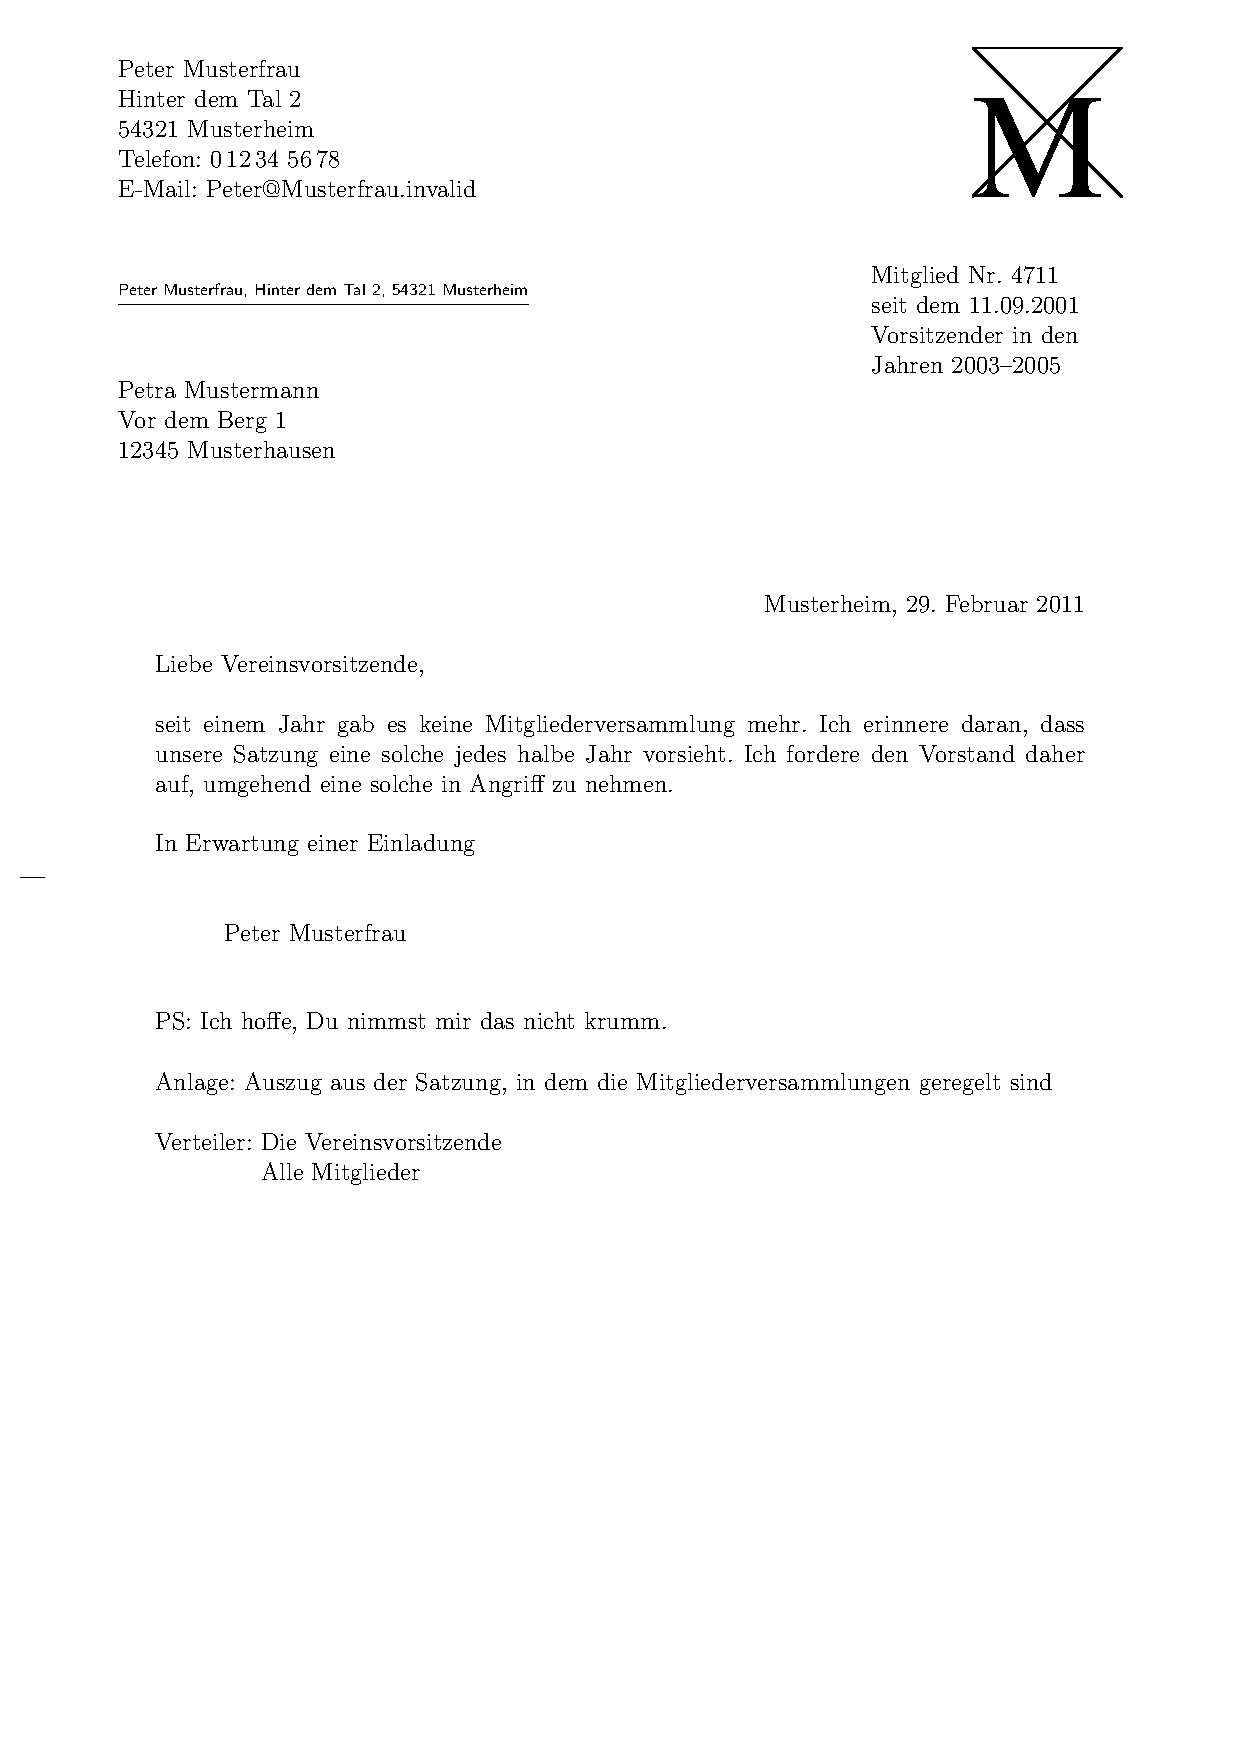
\includegraphics[width=.4\textwidth]{letter-example-20-de}}
    \end{captionbeside}
    \label{fig:\LabelBase.letter-20}
  \end{figure}
\end{Example}%
\EndIndexGroup
\EndIndexGroup
\EndIndexGroup
\ExampleEndFix% Beispiel am Ende der Beschreibung


\begin{Declaration}
  \PLength{refvpos}
\end{Declaration}
Diese Pseudolänge gibt den Abstand der Geschäftszeile von der Oberkante des
Papiers an. Ihr Wert wird in den vordefinierten
\File{lco}-Dateien\textnote{\File{lco}-Datei}\Index{lco-Datei=\File{lco}-Datei}
unterschiedlich eingestellt. %
\iffalse%
Typische Werte liegen zwischen 80{,}5\Unit{mm} und 98{,}5\Unit{mm}.%
\fi%
\EndIndexGroup


\begin{Declaration}
  \PLength{refwidth}
  \PLength{refhpos}
\end{Declaration}
Die Pseudolänge \PLength{refwidth} gibt die Breite an, die für die
Geschäftszeile zur Verfügung steht. Ihr Wert wird in den vordefinierten
\File{lco}-Dateien typischerweise auf 0\Unit{pt}
gesetzt. Dieser\textnote{Achtung!} Wert hat eine besondere Bedeutung. %
\iffalse% Umbruchoptimierung
Es wird damit keineswegs festgelegt, dass für die Geschäftszeile keine Breite
zur Verfügung steht. Vielmehr bedeutet der Wert%
\else%
Damit wird festgelegt%
\fi%
, dass die verfügbare Breite erst innerhalb von
\DescRef{\LabelBase.cmd.opening}\IndexCmd{opening} ermittelt wird.  Die%
\iffalse% Umbruchoptimierung
\ dort ermittelte %
\else%
se %
\fi%
Breite richtet sich \iffree{dann }{}nach der Einstellung der Option
\DescRef{\LabelBase.option.refline}\important{\DescRef{\LabelBase.option.refline}}%
\IndexOption{refline~=\PName{Einstellung}} (siehe
\DescPageRef{\LabelBase.option.refline}). Gleichzeitig wird 
\PLength{refhpos} entsprechend der Option gesetzt. Bei
\OptionValueRef{scrlttr2}{refline}{wide}%
\IndexOption{refline~=\textKValue{wide}} wird die Geschäftszeile zentriert,
wohingegen sie bei \OptionValueRef{scrlttr2}{refline}{narrow}%
\IndexOption{refline~=\textKValue{narrow}} am Satzspiegel links ausgerichtet
wird.

Ist \PLength{refwidth} von Null verschieden, wird die Breite der
Geschäftszeile nicht von der Option \DescRef{\LabelBase.option.refline}
bestimmt, sondern \PLength{refhpos} ist der Abstand der Geschäftszeile von der
linken Papierkante. Ist\textnote{Achtung!} dieser Abstand Null, so wird die
Geschäftszeile so ausgerichtet, dass das Verhältnis zwischen ihrem Abstand von
der linken Papierkante zu ihrem Abstand von der rechten Papierkante dem
Verhältnis zwischen den Abständen des Satzspiegels von der linken und rechten
Papierkante entspricht. Bei auf dem Papier horizontal zentriertem Satzspiegel
wird also auch die Geschäftszeile zentriert.

In der Regel werden diese Sonderfälle für die %
\iffalse% Umbruchkorrektur
häufigsten Anwendungen %
\else %
meisten Anwender %
\fi %
von geringem Interesse sein. Die\textnote{Tipp!} einfachste Regel lautet hier:
Entweder wird \PLength{refwidth} auf Null belassen und die Breite und
Ausrichtung der Geschäftszeile über die Option
\DescRef{\LabelBase.option.refline} bestimmt oder sowohl \PLength{refwidth} als
auch \PLength{refhpos} werden vom Anwender vorgegeben.%
\EndIndexGroup


\begin{Declaration}
  \PLength{refaftervskip}
\end{Declaration}
Diese Pseudolänge gibt den vertikalen Abstand an, der nach der Geschäftszeile
eingefügt werden soll. Der Wert wird in den vordefinierten
\File{lco}-Dateien\textnote{\File{lco}-Datei}\Index{lco-Datei=\File{lco}-Datei}
eingestellt. Er wirkt sich unmittelbar auf die Höhe des Textbereichs der
ersten Seite aus.%
\iffalse % Umbruchkorrektur
\ Der typische Wert liegt zwischen einer und zwei Zeilen.%
\fi %
\EndIndexGroup
%
\EndIndexGroup


\subsection{Titel und Betreff}
\seclabel{subject}%
\BeginIndexGroup
\BeginIndex{}{Betreff}

Der Betreff eine Briefes wird in unterschiedlichen Ländern unterschiedlich
gesetzt. Die einen haben ihn gerne vor der Anrede, die anderen setzen ihn
danach. Einige Berufsgruppen wollen ihn teilweise sogar vor der Geschäftszeile
haben.


\begin{Declaration}
  \Variable{title}
\end{Declaration}
Bei \KOMAScript{} kann ein Brief zusätzlich mit einem Titel\Index{Titel}
versehen werden. Der Titel wird zentriert in der Schriftgröße \Macro{LARGE}
unterhalb der Geschäftszeile ausgegeben.

\BeginIndex{FontElement}{lettertitle}\LabelFontElement{lettertitle}%
\BeginIndex{FontElement}{title}\LabelFontElement{title}%
Die Schriftart für das Element\ChangedAt{v3.17}{\Class{scrlttr2}\and
  \Package{scrletter}} \FontElement{lettertitle}%
\important{\FontElement{lettertitle}} kann mit den Anweisungen
\DescRef{\LabelBase.cmd.setkomafont} und
\DescRef{\LabelBase.cmd.addtokomafont} (siehe
\autoref{sec:\LabelBase.textmarkup} ab
\DescPageRef{\LabelBase.cmd.setkomafont}) geändert werden. Dabei sind auch
Größenangaben erlaubt. Die Größe \Macro{LARGE} wird der Schriftauswahl
innerhalb von \KOMAScript{} immer vorangestellt und ist daher auch nicht
Teil\textnote{Voreinstellung} der Voreinstellung
\ChangedAt{v3.39}{\Class{scrlttr2}}\Macro{normalcolor}""%
\DescRef{\LabelBase.cmd.maybesffamily}\IndexCmd{maybesffamily}""%
\Macro{bfseries}. Bei
\Class{scrlttr2}\OnlyAt{\Class{scrlttr2}} kann als Alias für
\FontElement{lettertitle} auch
\FontElement{title}\important{\FontElement{title}} verwendet werden. Bei
Verwendung von \Package{scrletter} mit einer \KOMAScript-Klasse ist das
nicht\textnote{Achtung!} möglich, da bei diesen Klassen bereits ein Element
\FontElement{title} mit abweichender Einstellung für den Dokumenttitel
existiert.%
\EndIndex{FontElement}{title}%
\EndIndex{FontElement}{lettertitle}%
\begin{Example}
  Angenommen, Sie schreiben eine Mahnung. Sie setzen einen
  entsprechenden Titel:
\begin{lstcode}
  \setkomavar{title}{Mahnung}
\end{lstcode}
  Damit sollte der Empfänger die Mahnung als solche erkennen.
\end{Example}
Während der \PName{Inhalt} der Variablen, wie im Beispiel gezeigt, den Titel
definiert, wird die \PName{Bezeichnung} der Variablen \Variable{title} von
\KOMAScript{} nicht genutzt.
%
\EndIndexGroup


\begin{Declaration}
  \OptionVName{subject}{Einstellung}
  \Variable{subject}
  \Variable{subjectseparator}
\end{Declaration}
\BeginIndex{}{Betreff}%
Um einen Betreff zu setzen, legt man den \PName{Inhalt} der Variablen
\Variable{subject} entsprechend fest. Mit Option
\OptionValue{subject}{titled}\important{\OptionValue{subject}{titled}} kann
dann zum einen gewählt werden, dass der Betreff mit einem Titel versehen
werden soll oder nicht. Der Titel wird über die Bezeichnung der Variablen
\Variable{subject} bestimmt (siehe \autoref{tab:\LabelBase.subjectTerm}).
Der\textnote{Voreinstellung} vordefinierte Inhalt des
Trennzeichens\Index{Trennzeichen} \Variable{subjectseparator} besteht aus
einem Doppelpunkt, gefolgt von einem Leerzeichen.  Zum%
\important{\OptionValue{subject}{afteropening}\\
  \OptionValue{subject}{beforeopening}}
anderen kann über
\OptionValue{subject}{afteropening}
gewählt werden, dass der Betreff
abweichend von der Voreinstellung \OptionValue{subject}{beforeopening} erst
nach der Anrede gesetzt werden soll. Eine%
\important{\OptionValue{subject}{underlined}\\
  \OptionValue{subject}{centered}\\
  \OptionValue{subject}{right}} andere Formatierung kann mit
\OptionValue{subject}{underlined} und \OptionValue{subject}{centered} oder
\OptionValue{subject}{right}\ChangedAt{v2.97c}{\Class{scrlttr2}} eingestellt
werden.

\begin{table}
%  \centering
  \KOMAoptions{captions=topbeside}%
  \setcapindent{0pt}%
%  \caption
  \begin{captionbeside}
    [{Vordefinierte Bezeichnungen der Variablen für den Betreff}]
    {\hspace{0pt plus 1ex}%
      Vordefinierte Bezeichnungen der Variablen für den Betreff}
    [l]
    \begin{tabular}[t]{lll}
      \toprule
      Name               & Bezeichnung \\
      \midrule
      \Variable{subject} & \DescRef{\LabelBase.cmd.usekomavar*}\PParameter{subjectseparator}%
                           \texttt{\%} \\ 
                         & \texttt{\quad}%
                           \DescRef{\LabelBase.cmd.usekomavar}\PParameter{subjectseparator} \\
      \Variable{subjectseparator} & \DescRef{scrlttr2-experts.cmd.subjectname} \\
      \bottomrule
    \end{tabular}
  \end{captionbeside}
  \label{tab:\LabelBase.subjectTerm}
\end{table}

Mögliche Werte für Option \Option{subject} sind
\autoref{tab:\LabelBase.subject} zu entnehmen. %
\iffalse% Umbruchkorrektur
Es wird ausdrücklich\textnote{Achtung!} darauf hingewiesen, dass bei der
Einstellung \OptionValue{subject}{underlined} der Betreff komplett in eine
Zeile passen muss!%
\else%
Es wird\textnote{Achtung!} darauf hingewiesen, dass bei Einstellung
\OptionValue{subject}{underlined} der Betreff in eine Zeile passen muss!%
\fi%
\begin{table}
%  \centering
  \KOMAoptions{captions=topbeside}%
  \setcapindent{0pt}%
%  \caption
  \begin{captionbeside}
    [{Mögliche Werte für Option \Option{subject}}]
    {\hspace{0pt plus 1ex}%
      Mögliche Werte für Option \Option{subject} zur Platzierung und
      Formatierung eines Betreffs%
      \label{tab:\LabelBase.subject}}
    [l]
    \begin{minipage}[t]{.667\linewidth}
      \begin{desctabular}[t]
        \pventry{afteropening}{Betreff nach der Anrede setzen.}\\[-1.7ex]
        \pventry{beforeopening}{Betreff vor der Anrede setzen
          (Voreinstellung).}\\[-1.7ex]
        \pventry{centered}{Betreff zentrieren.}\\[-1.7ex]
        \pventry{left}{Betreff linksbündig setzen (Voreinstellung).}\\[-1.7ex]
        \pventry{right}{Betreff rechtsbündig setzen.}\\[-1.7ex]
        \pventry{titled}{Betreff mit Titel versehen.}\\[-1.7ex]
        \pventry{underlined}{Betreff unterstreichen. (Hinweis im Text
          beachten!)}\\[-1.7ex]
        \pventry{untitled}{Betreff nicht mit Titel versehen (Voreinstellung).}%
      \end{desctabular}
    \end{minipage}
  \end{captionbeside}
\end{table}

\BeginIndexGroup
\BeginIndex{FontElement}{lettersubject}\LabelFontElement{lettersubject}%
\BeginIndex{FontElement}{subject}\LabelFontElement{subject}%
Der Betreff wird in einer eigenen Schriftart\Index{Schrift>Art} gesetzt. Um
diese zu ändern, verwenden Sie die Anweisungen
\DescRef{\LabelBase.cmd.setkomafont} und
\DescRef{\LabelBase.cmd.addtokomafont} (siehe
\autoref{sec:\LabelBase.textmarkup} ab
\DescPageRef{\LabelBase.cmd.setkomafont}). Für das
Element\ChangedAt{v3.17}{\Class{scrlttr2}\and \Package{scrletter}}
\FontElement{lettersubject}\important{\FontElement{lettersubject}} ist als
Schrift \Macro{normalcolor}\Macro{bfseries} voreingestellt. Bei Klasse
\Class{scrlttr2}\OnlyAt{\Class{scrlttr2}} kann als Alias für
\FontElement{lettersubject} auch
\FontElement{subject}\important{\FontElement{subject}} verwendet werden. Bei
Verwendung von Paket \Package{scrletter} mit einer \KOMAScript-Klasse ist das
nicht\textnote{Achtung!} möglich, da bei diesen Klassen bereits ein Element
\FontElement{subject} mit abweichender Einstellung für den Dokumenttitel
existiert.
\EndIndexGroup

\begin{Example}
  Herr Musterfrau setzt nun auch den Betreff. %
  \iftrue % Umbruchkorrektur
  Als eher traditioneller veranlagter Mensch möchte er %
  \else %
  Er möchte %
  \fi %
  außerdem, dass der Betreff mit einer %
  \iftrue % Umbruchkorrektur
  entsprechenden %
  \fi %
  Spitzmarke versehen wird, und setzt deshalb auch die zugehörige Option:%
  \lstinputcode[xleftmargin=1em]{letter-example-21-de.tex}%
  Das Ergebnis ist in \autoref{fig:\LabelBase.letter-21} zu sehen.
  \begin{figure}
    \setcapindent{0pt}%
    \begin{captionbeside}[{Beispiel: Brief mit erweitertem Absender, Logo,
        Anschrift, Absenderergänzung, Ort, Datum, Betreff, Anrede, Text,
        Grußfloskel, Signatur, Postskriptum, Anlagen, Verteiler und
        Lochermarke}]{Ergebnis eines kleinen Briefes mit erweitertem Absender,
        Logo, Anschrift, Absenderergänzung, Ort, Datum, Betreff,
        Anrede, Text, Grußfloskel, Signatur, Postskriptum, Anlagen, Verteiler
        und Lochermarke}[l]
      \frame{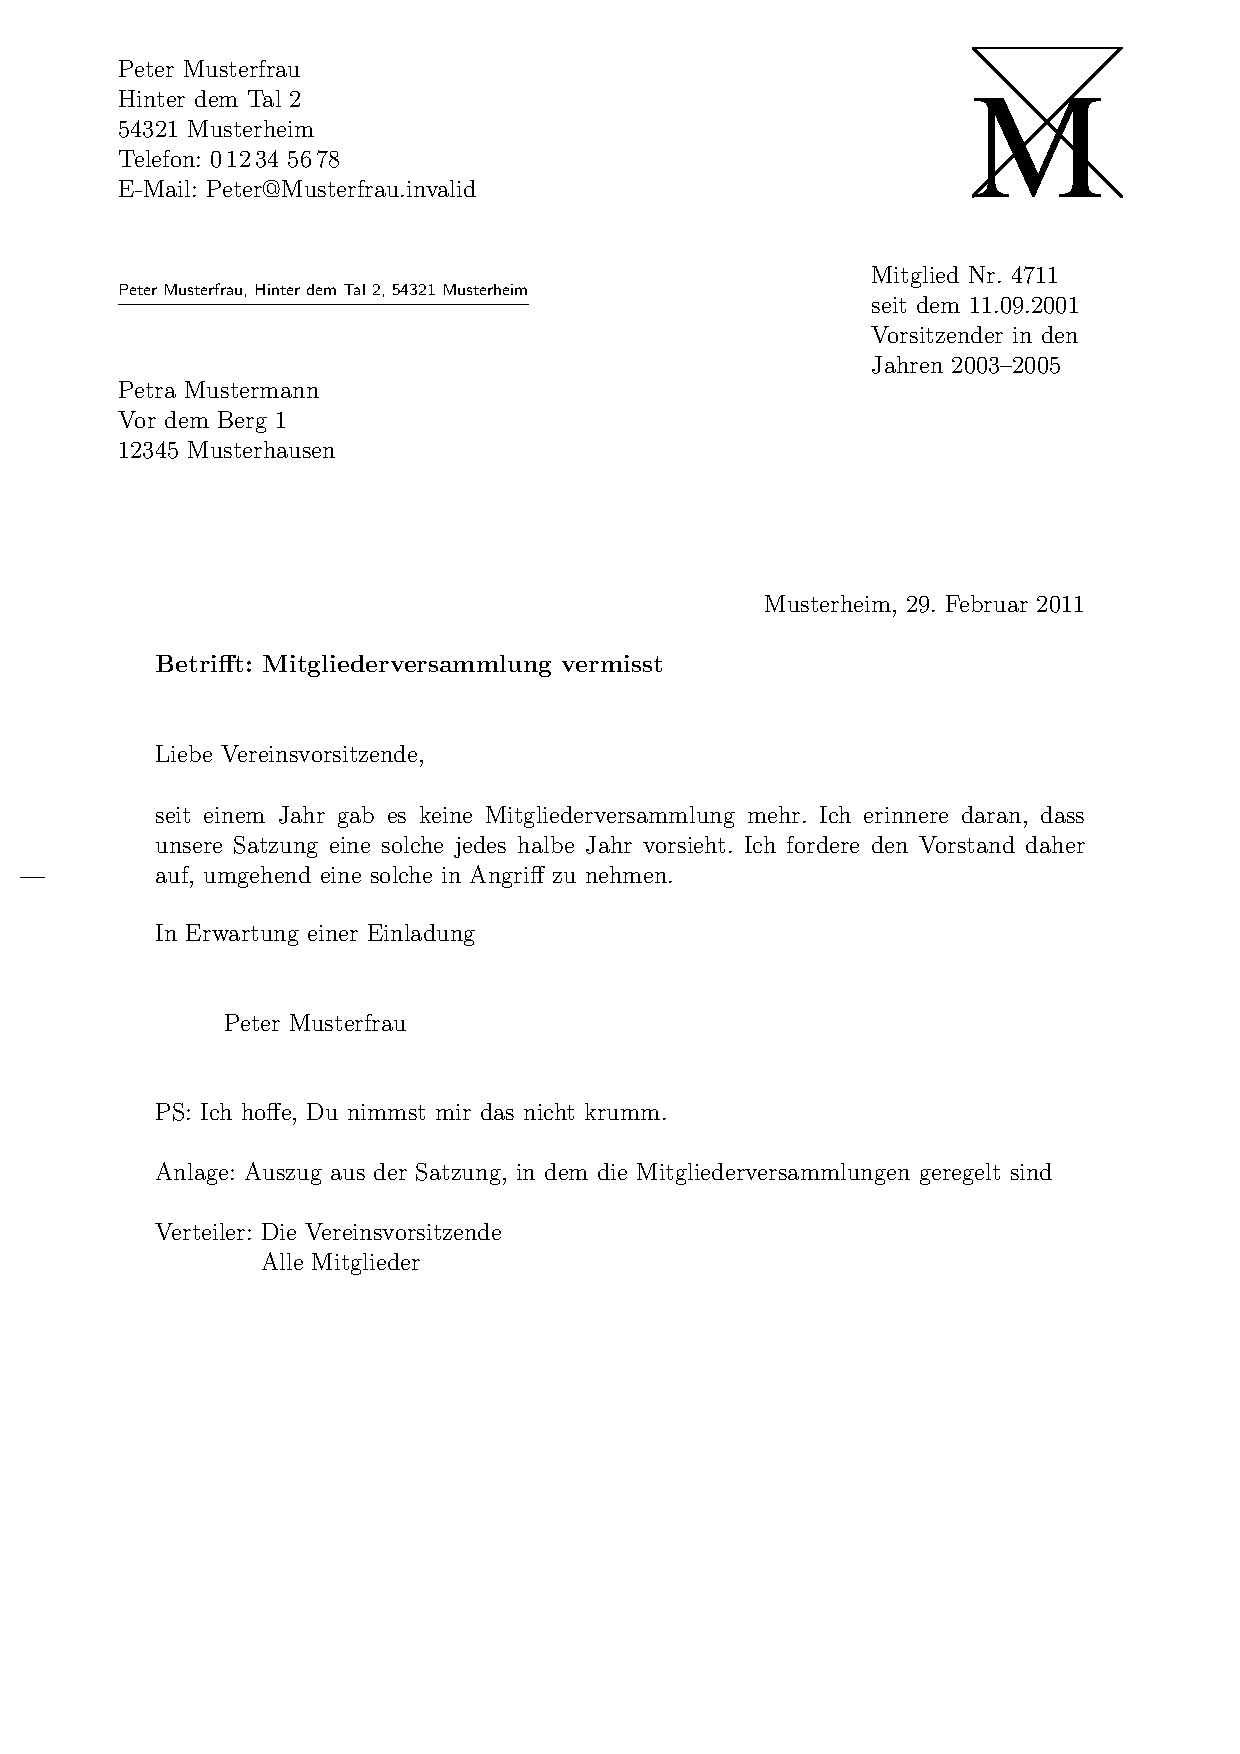
\includegraphics[width=.4\textwidth]{letter-example-21-de}}
    \end{captionbeside}
    \label{fig:\LabelBase.letter-21}
  \end{figure}
\end{Example}
Voreingestellt\textnote{Voreinstellung} sind
\OptionValue{subject}{beforeopening}, \OptionValue{subject}{left} sowie
\OptionValue{subject}{untitled}.%
\EndIndexGroup

\begin{Declaration}
  \PLength{subjectvpos}
\end{Declaration}
\ChangedAt{v3.01}{\Class{scrlttr2}}%
Ist\textnote{Achtung!} der Wert dieser Pseudolänge 0\Unit{pt}, so bestimmt die
Option
\DescRef{\LabelBase.option.subject}\important{\DescRef{\LabelBase.option.subject}}%
\IndexOption{subject~=\PName{Einstellung}} (siehe
\DescPageRef{\LabelBase.option.subject}) die
Position des Betreffs. Dabei spielen dann auch die nachfolgend erklärten
Pseudolängen \DescRef{\LabelBase.plength.subjectbeforevskip} und \DescRef{\LabelBase.plength.subjectaftervskip} ihre
Rolle. Bei allen anderen Werten wird der Betreff mit dem entsprechenden
Abstand von der oberen Papierkante platziert. Es\textnote{Tipp!} wird
empfohlen in diesem Fall darauf zu achten, dass genügend Platz zur Verfügung
steht, damit Überschneidungen mit anderen Elementen unwahrscheinlich sind.
\begin{Example}
  Einige wenige Berufsgruppen ziehen es vor, wenn der Betreff noch vor der
  Geschäftszeile steht. Hierzu kann man die Position wie folgt wählen, wobei
  auch die Position der Geschäftszeile angepasst wird:
\begin{lstcode}
  \ProvidesFile{lawsubj.lco}
               [2008/11/03 lawyers lco file]
  \setplength{subjectvpos}{\useplength{refvpos}}
  \addtoplength{refvpos}{3\baselineskip}
  \endinput
\end{lstcode}
  Will man, dass zwischen Betreff und Geschäftszeile noch mindestens eine
  Zeile frei bleibt, hat man so Platz für maximal zwei Zeilen Betreff.%
  \iftrue % Umbruchkorrektur
  \ Das sollte in den allermeisten Fällen genügen.%
  \fi%
\end{Example}
\EndIndexGroup
\ExampleEndFix


\begin{Declaration}
  \PLength{subjectbeforevskip}
  \PLength{subjectaftervskip}
\end{Declaration}
\ChangedAt{v3.01}{\Class{scrlttr2}}%
Wird der Betreff nicht absolut platziert, sondern vor oder nach der Anrede, so
kann vor und nach dem Betreff ein zusätzlicher Abstand eingefügt werden. Der
Abstand vor dem Betreff trifft dabei gegebenenfalls mit anderen Abständen,
etwa dem automatischen Abstand von einer Zeile nach dem Titel, zusammen. In
der Voreinstellung\textnote{Voreinstellung} wird daher in der Regel kein
weiterer Abstand an dieser Stelle eingefügt. Der Abstand nach dem Betreff
beträgt in der Voreinstellung von Klasse und Paket zwei Zeilen.%
\EndIndexGroup
% 
\EndIndexGroup


\subsection{Schlussgruß}
\seclabel{closing}
\BeginIndexGroup
\BeginIndex{}{Schlussgruss=Schlussgruß}%
\BeginIndex{}{Gruss=Gruß}

Dass der Schlussgruß mit \DescRef{\LabelBase.cmd.closing}\IndexCmd{closing}
gesetzt wird, wurde bereits in \autoref{sec:\LabelBase.document},
\DescPageRef{\LabelBase.cmd.closing} erklärt. %
\iffalse % Umbruchkorrektur
Unter dem Schlussgruß wird häufig noch eine Signatur, eine Art Erläuterung zur
Unterschrift, gesetzt. Die Unterschrift wiederum findet Platz zwischen dem
Schlussgruß und der Signatur.%
\else%
Unter Schlussgruß und Unterschrift wird häufig noch eine Signatur als eine Art
Erläuterung oder Klartext der Unterschrift gesetzt.%
\fi%

\begin{Declaration}
  \Variable{signature}
\end{Declaration}
Die Variable \Variable{signature}\Index{Signatur} nimmt eine Art Erläuterung
zur Unterschrift\Index{Unterschrift} auf. Ihr \PName{Inhalt} ist mit
\DescRef{\LabelBase.cmd.usekomavar}\PParameter{fromname} vordefiniert. Eine
solche Erläuterung kann auch mehrzeilig sein. Die einzelnen Zeilen sollten
dann mit doppeltem Backslash voneinander getrennt
werden. Absätze\textnote{Achtung!} innerhalb der Erläuterung sind jedoch nicht
gestattet.%
%
\EndIndexGroup


\begin{Declaration}
  \Macro{raggedsignature}
\end{Declaration}
Grußfloskel\Index{Gruss=Gruß}\Index{Signatur} und Erläuterung der
Unterschrift\Index{Unterschrift} werden innerhalb einer gemeinsamen Box
gesetzt.  Die Breite dieser Box wird durch die längste Zeile innerhalb von
Grußfloskel und Erläuterung bestimmt.

Wo genau diese Box platziert wird, ist durch die Pseudolängen
\DescRef{\LabelBase.plength.sigindent}\IndexPLength{sigindent} und
\DescRef{\LabelBase.plength.sigbeforevskip}\IndexPLength{sigbeforevskip}
(siehe \DescPageRef{\LabelBase.plength.sigindent}) bestimmt.  Durch den Befehl
\Macro{raggedsignature} wird die Ausrichtung innerhalb der Box bestimmt. In
den vordefinierten\textnote{Voreinstellung} \File{lco}-Dateien ist die
Anweisung entweder auf \Macro{centering} oder
auf \Macro{raggedright} (nur \Option{KOMAold}) gesetzt. Um innerhalb der Box
beispielsweise eine linksbündige oder rechtsbündige Ausrichtung zu erhalten,
kann der Befehl in gleicher Weise umdefiniert werden wie
\DescRef{maincls.cmd.raggedsection} (siehe %
\iffalse % Umbruchkorrektur
das entsprechende Beispiel in %
\fi %
\autoref{sec:maincls.structure}, \DescPageRef{maincls.cmd.raggedsection}).

\begin{Example}
  Herr Musterfrau will sich nun wirklich wichtig machen und deshalb in der
  Signatur nochmals darauf hinweisen, dass er selbst schon Vereinsvorsitzender
  war. Deshalb ändert er die Variable
  \DescRef{\LabelBase.variable.signature}. Außerdem will er, dass die Signatur
  linksbündig unter dem Schlussgruß steht, und definiert dazu
  \Macro{raggedsignature} um:%
  {\phantomsection\xmpllabel{letterwithoutlco}}%
  \lstinputcode[xleftmargin=1em]{letter-example-22-de}%
  Das Ergebnis ist in \autoref{fig:\LabelBase.letter-22} zu sehen.%
  \iffalse % Umbruchkorrektur (Achtung wegen unten!)
  Dieses Beispiel zeigt die wichtigsten Elemente des Briefbogens und kann so
  als Muster für eigene Briefe dienen.%
  \fi %
  \begin{figure}
    \setcapindent{0pt}%
    \begin{captionbeside}[{Beispiel: Brief mit erweitertem Absender, Logo,
        Anschrift, Absenderergänzung, Ort, Datum, Betreff, Anrede, Text,
        Grußfloskel, geänderter Signatur, Postskriptum, Anlagen, Verteiler und
        Lochermarke}]{Ergebnis eines kleinen Briefes mit erweitertem Absender,
        Logo, Anschrift, Absenderergänzung, Ort, Datum, Betreff,
        Anrede, Text, Grußfloskel, geänderter Signatur, Postskriptum, Anlagen,
        Verteiler und Lochermarke}[l]
      \frame{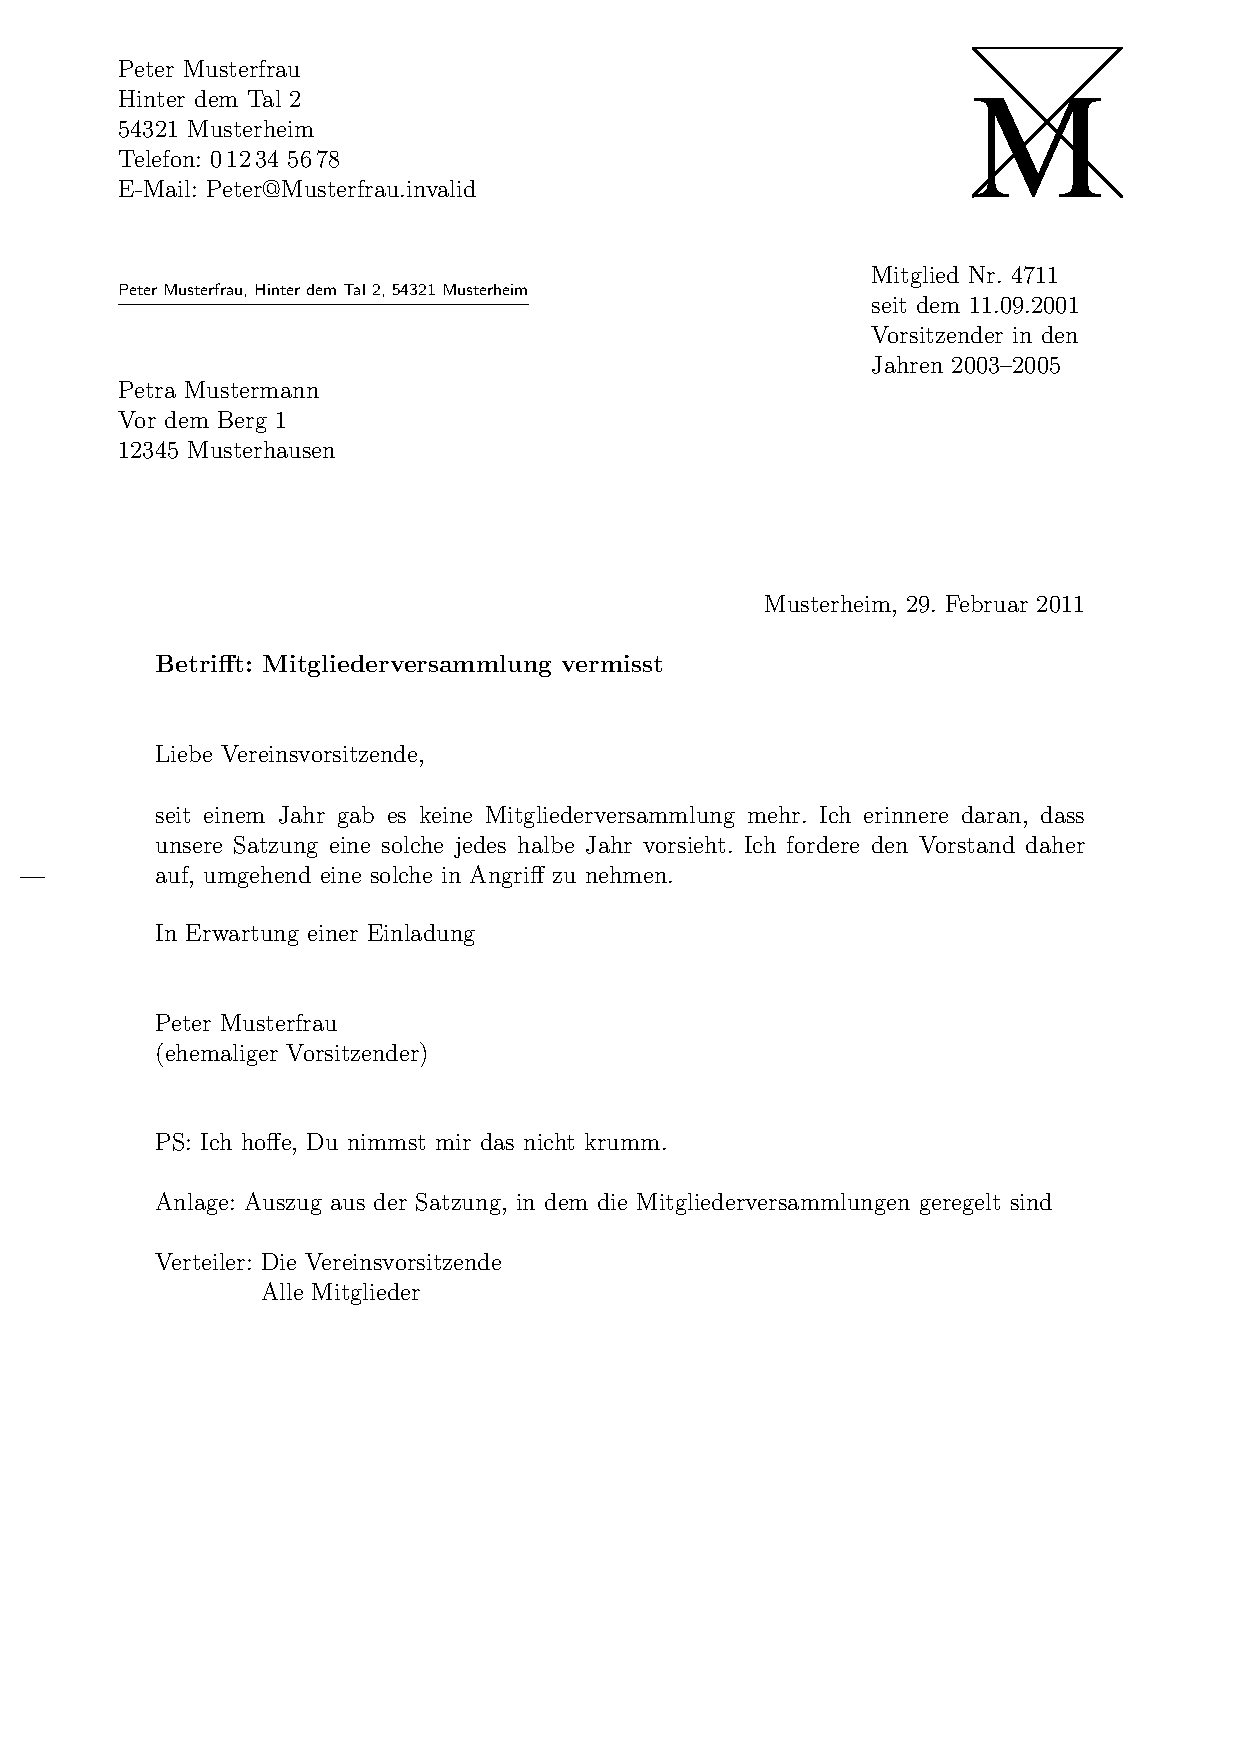
\includegraphics[width=.4\textwidth]{letter-example-22-de}}
    \end{captionbeside}
    \label{fig:\LabelBase.letter-22}
  \end{figure}
\end{Example}
\iffalse% Umbruchkorrekturtext (Achtung wegen oben!)
  Das vorausgehende Beispiel zeigt die wichtigsten, aber nicht alle möglichen
  Elemente eines Briefes. Es kann jedoch sehr gut als allgemeines Muster
  dienen.%
\else
  \ExampleEndFix% Beispiel am Ende der Erklärung  
\fi
%
\EndIndexGroup


\begin{Declaration}
  \PLength{sigindent}
  \PLength{sigbeforevskip}
\end{Declaration}
Grußfloskel\Index{Gruss=Gruß}\Index{Signatur} und Erläuterung der
Unterschrift\Index{Unterschrift} werden innerhalb einer Box gesetzt.  Die
Breite dieser Box wird durch die längste Zeile innerhalb von Grußfloskel und
Erläuterung bestimmt.

Die Box wird mit dem durch die Pseudolänge \PLength{sigindent} festgelegten
Einzug gesetzt. In den vordefinierten\textnote{Voreinstellung}
\File{lco}-Dateien ist der Einzug auf 0\Unit{mm} gesetzt.

Zwischen Grußfloskel und Erläuterung wird ein vertikaler Abstand eingefügt,
der mit der Pseudolänge \PLength{sigbeforevskip} festgelegt ist. In den
vordefinierten\textnote{Voreinstellung} \File{lco}-Dateien ist der Wert auf
zwei Zeilen eingestellt. In diese Lücke setzen Sie dann Ihre Unterschrift.%
\iffalse% Umbruchkorrekturtext
\ Sollten\textnote{Tipp!} Sie sich dazu entschließen in die Variable
\DescRef{\LabelBase.variable.signature}\IndexVariable{signature}%
\important{\DescRef{\LabelBase.variable.signature}} mit Paket
\Package{graphicx}\IndexPackage{graphicx} ein Faksimile Ihrer Unterschrift
einzufügen, wäre es also sinnvoll den Wert von \PLength{sigbeforevskip} und
damit die Lücke zwischen Schlussgruß und Signatur zu verringern.%
\fi%
\EndIndexGroup
% 
\EndIndexGroup


\subsection{Briefbogenfuß}
\seclabel{firstFoot}%
\BeginIndexGroup
\BeginIndex{}{Briefbogenfuss=Briefbogenfuß}%

Die erste Seite eines Briefes, der Briefbogen, enthält nicht nur einen eigenen
Kopf, den Briefkopf. Diese Seite enthält auch einen eigenen
Fuß\Index{Fuss=Fuß}, den Briefbogenfuß. %
\iftrue% Umbruchvarianten
Dieser wird ebenfalls nicht über den Seitenstil%
\else%
Genau wie der Briefkopf wird der Briefbogenfuß nicht über den Seitenstil%
\fi%
, sondern unmittelbar von \DescRef{\LabelBase.cmd.opening}\IndexCmd{opening}%
\important{\DescRef{\LabelBase.cmd.opening}} ausgegeben.


\begin{Declaration}
  \OptionVName{enlargefirstpage}{Ein-Aus-Wert}
\end{Declaration}
\begin{Explain}
  Die erste Seite eines Briefes fällt %
  \iftrue % Umbruchkorrektur
    aufgrund der vielen Konsultationselemente, wie dem Briefkopf oder der
    Anschrift,
    % 
  \fi %
  immer aus dem normalen Satzspiegel. Von \KOMAScript{} werden Mechanismen
  bereitgestellt, um die Höhe und vertikale Ausrichtung von Kopf und Fuß der
  ersten Seite unabhängig von den Folgeseiten zu bestimmen. Würde dadurch der
  Fuß der ersten Seite in den Textbereich\Index{Text>Bereich} ragen, so wird
  der Textbereich der ersten Seite automatisch mit Hilfe von
  \Macro{enlargethispage}\IndexCmd{enlargethispage} verkleinert. 
\end{Explain}
Soll der Textbereich auch automatisch mit \Macro{enlargethispage} vergrößert
werden, falls der Fuß der ersten Seite dies erlaubt, so kann das mit dieser
Option erreicht werden. Es passt dann bestenfalls etwas mehr Text auf die
erste Seite.  Siehe hierzu auch die Erklärung zur Pseudolänge
\DescRef{\LabelBase.plength.firstfootvpos} auf
\DescPageRef{\LabelBase.plength.firstfootvpos}. Als \PName{Ein-Aus-Wert} kann
einer der Standardwerte für einfache Schalter aus
\autoref{tab:truefalseswitch}, \autopageref{tab:truefalseswitch} verwendet
werden. Voreingestellt\textnote{Voreinstellung} ist
\PValue{false}.%
\EndIndexGroup


\begin{Declaration}
  \OptionVName{firstfoot}{Ein-Aus-Wert}
\end{Declaration}
\BeginIndex{}{Briefbogenfuss=Briefbogenfuß}%
Diese\ChangedAt{v2.97e}{\Class{scrlttr2}} Option bestimmt, ob der
Briefbogenfuß überhaupt gesetzt wird. Das Abschalten mit
\OptionValue{firstfoot}{false}\important{\OptionValue{firstfoot}{false}} hat
Auswirkungen wenn gleichzeitig die zuvor dokumentierte Option
\DescRef{\LabelBase.option.enlargefirstpage} verwendet wird, da sich
dadurch die Seite logisch nach unten verlängert. Zwischen dem Ende des
Satzspiegels und dem Seitenende bleibt dann nur der normale Abstand zwischen
Satzspiegel und Seitenfuß.

Die Option versteht die Standardwerte für einfache Schalter, die in
\autoref{tab:truefalseswitch}, \autopageref{tab:truefalseswitch} angegeben
sind. Voreingestellt\textnote{Voreinstellung} ist das Setzen des
Briefbogenfußes.%
\EndIndexGroup


\begin{Declaration}
  \Variable{firstfoot}
\end{Declaration}%
\BeginIndex{}{Briefbogenfuss=Briefbogenfuß}%
\iffalse % Umbruchkorrektur
Der Fuß der ersten Seite ist in der Voreinstellung\textnote{Voreinstellung}
leer.  Es besteht jedoch die Möglichkeit, über den \PName{Inhalt} der
Variablen\ChangedAt{v3.08}{\Class{scrlttr2}} \Variable{firstfoot} einen neue
Festlegung zu treffen. %
\else %
Der Inhalt der Variablen\ChangedAt{v3.08}{\Class{scrlttr2}}
\Variable{firstfoot} und damit des Fußes der ersten Seite ist in der
Voreinstellung\textnote{Voreinstellung} leer. %
\fi %
Die \PName{Bezeichnung} der Variablen wird von \KOMAScript{} nicht genutzt.

\BeginIndex{Variable}{frombank}%
\begin{Example}
  Sie wollen den Inhalt der Variablen \DescRef{\LabelBase.variable.frombank},
  also die Bankverbindung, im Fuß der ersten Seite ausgeben. Der doppelte
  Backslash soll dabei durch ein Komma ersetzt werden:
\begin{lstcode}
  \setkomavar{firstfoot}{%
    \parbox[b]{\linewidth}{%
      \centering\def\\{, }\usekomavar{frombank}%
    }%
  }
\end{lstcode}
  Natürlich können Sie für das Trennzeichen auch eine eigene Variable
  definieren.%
  \iffalse % Umbruchkorrektunr
  Ich überlasse dem Leser dies als Übung.%
  \fi%
  
  Will man eine Art Brief"|fuß als Gegengewicht zum Briefkopf verwenden, so
  kann dieser beispielsweise wie folgt definiert werden:
\begin{lstcode}
  \setkomavar{firstfoot}{%
    \parbox[t]{\textwidth}{\footnotesize
      \begin{tabular}[t]{l@{}}%
        \multicolumn{1}{@{}l@{}}{Gesellschafter:}\\
        Hugo Mayer\\
        Bernd Müller
      \end{tabular}%
      \hfill
      \begin{tabular}[t]{l@{}}%
        \multicolumn{1}{@{}l@{}}{Geschäftsführung:}\\
        Liselotte Mayer\\[1ex]
        \multicolumn{1}{@{}l@{}}{Gerichtsstand:}\\
        Hinterdupfeldingen
      \end{tabular}%
      \Ifkomavarempty{frombank}{}{%
        \hfill
        \begin{tabular}[t]{l@{}}%
          \multicolumn{1}{@{}l@{}}{%
            \usekomavar*{frombank}:}\\
          \usekomavar{frombank}
        \end{tabular}%
        }%
      }%
    }
\end{lstcode}
  Das Beispiel stammt ursprünglich von Torsten Krüger. Es wird empfohlen, eine
  solche Definition für die mehrfache Verwendung in unterschiedlichen
  Dokumenten in einer eigenen
  \File{lco}-Datei\Index{lco-Datei=\File{lco}-Datei} abzulegen. Mit
\begin{lstcode}
  \setkomavar{frombank}{IBAN DE21~87654321~13456789\\
                        bei der HansWurstBank\\
                        BIC GRMLDEHD000}
\end{lstcode}
  kann die Bankverbindung dann im Dokument passend dazu gesetzt werden.%
\iffalse% Umbruchkorrekturmöglichkeit
  \ Abhängig\textnote{Achtung!} von den Voreinstellungen ist ein solch hoher
  Fuß jedoch eventuell nicht vorgesehen und wird deshalb möglicherweise zu
  tief platziert. In einem solchen Fall kann die vertikale Position über die
  Pseudolänge \DescRef{\LabelBase.plength.firstfootvpos}%
  \important{\DescRef{\LabelBase.plength.firstfootvpos}}%
  \IndexPLength{firstfootvpos} angepasst werden (siehe
  \DescPageRef{\LabelBase.plength.firstfootvpos}).%
\fi
\end{Example}

Im\textnote{Achtung!} Beispiel wurde ein mehrzeiliger Fuß gesetzt. Bei einer
Kompatibilitätseinstellung ab Version
2.9u\important{\OptionValueRef{\LabelBase}{version}{2.9u}} (siehe
\DescRef{\LabelBase.option.version} in
\autoref{sec:\LabelBase.compatibilityOptions},
\DescPageRef{\LabelBase.option.version}) reicht der Platz dafür in der Regel
nicht aus. Sie sollten dann \DescRef{\LabelBase.plength.firstfootvpos} (siehe
\DescPageRef{\LabelBase.plength.firstfootvpos}) entsprechend
verringern.%
\EndIndexGroup

\begin{Declaration}
  \Variable{frombank}
\end{Declaration}%
\BeginIndex{}{Briefbogenfuss=Briefbogenfuß} Die im vorherigen Beispiel
verwendete Variable \Variable{frombank} nimmt derzeit eine Sonderstellung
ein. Sie wird intern bisher nicht verwendet. Sie kann jedoch vom Anwender
verwendet werden, um die Bankverbindung\Index{Bankverbindung} in das
Absenderergänzungsfeld (siehe Variable \DescRef{\LabelBase.variable.location},
\DescPageRef{\LabelBase.variable.location}) oder wie im Beispiel in den Fuß zu
setzen.%
%
\EndIndexGroup

\begin{Declaration}
  \PLength{firstfootvpos}
\end{Declaration}
Diese Pseudolänge gibt den Abstand des Fußes der ersten Briefseite von der
Oberkante des Papiers an. Es wird außerdem dafür gesorgt, dass der Textbereich
nicht in den Fuß hineinragt. Hierzu wird auf der ersten Seite gegebenenfalls
die Höhe des Textbereichs mit Hilfe von
\Macro{enlargethispage}\IndexCmd{enlargethispage}%
\important{\Macro{enlargethispage}} verkleinert. Mit Hilfe der Option
\DescRef{\LabelBase.option.enlargefirstpage}%
\important{\DescRef{\LabelBase.option.enlargefirstpage}} (siehe
\DescPageRef{\LabelBase.option.enlargefirstpage}) kann dafür gesorgt werden,
dass die Höhe des Textbereichs umgekehrt gegebenenfalls auch vergrößert
wird. Damit kann dann der Abstand zwischen Textbereich und Fuß der ersten
Seite auf den Wert der Länge
\Length{footskip}\IndexLength{footskip}\important{\Length{footskip}}
verringert werden.

Bei\textnote{\OptionValueRef{\LabelBase}{version}{2.9t}}
Kompatibilitätseinstellungen\ChangedAt{v2.9t}{\Class{scrlttr2}} bis
Version~2.9t (siehe \DescRef{\LabelBase.option.version} in
\autoref{sec:\LabelBase.compatibilityOptions},
\DescPageRef{\LabelBase.option.version}) wird außer bei \Option{KOMAold} und
\Option{NF} in allen vordefinierten
\File{lco}-Dateien\textnote{\File{lco}-Datei}\Index{lco-Datei=\File{lco}-Datei}
(siehe \autoref{sec:\LabelBase.lcoFile}) der Fuß abhängig vom Satzspiegel
gesetzt%
\iffalse % Umbruchkorrektur
. Damit hat dann auch \DescRef{\LabelBase.option.enlargefirstpage}%
\important{\DescRef{\LabelBase.option.enlargefirstpage}} keine Wirkung. %
\else %
\ und \DescRef{\LabelBase.option.enlargefirstpage}%
\important{\DescRef{\LabelBase.option.enlargefirstpage}} ignoriert. %
\fi %
Ab
Version 2.9u bekommt der Fuß eine Position am unteren Ende des Papiers. Damit
ist dann die Höhe des Satzspiegels des Briefbogens eventuell auch von der
Option \DescRef{\LabelBase.option.enlargefirstpage} abhängig.

Wird der Briefbogenfuß mit Option
\OptionValueRef{scrlttr2}{firstfoot}{false}%
\important{\OptionValueRef{scrlttr2}{firstfoot}{false}}%
\IndexOption{firstfoot~=\textKValue{false}}\ChangedAt{v2.97e}{\Class{scrlttr2}}
(siehe \DescPageRef{\LabelBase.option.firstfoot}) abgeschaltet, so wird
\PLength{firstfootvpos} ignoriert und stattdessen
\Length{paperheight}\IndexLength{paperheight} angenommen. Es bleibt dann
ein minimaler unterer Rand von \Length{footskip}\IndexLength{footskip}.%
\EndIndexGroup


\begin{Declaration}
  \PLength{firstfoothpos}
\end{Declaration}
Die\textnote{Achtung!} Pseudolänge
\PLength{firstfoothpos}\ChangedAt{v3.05}{\Class{scrlttr2}} gibt bei einem
positiven Wert den Abstand des Briefbogenfußes von der linken Papierkante
an. Ist der Wert sogar größer oder gleich der Breite des Papiers,
\Length{paperwidth}\IndexLength{paperwidth}, so wird der Fuß horizontal
zentriert auf dem Briefbogen platziert. Ein negativer Wert gibt den Abstand
des Fußes von der rechten Papierkante an. Ist der Wert jedoch kleiner oder
gleich der negativen Breite des Papiers, so wird der Fuß bündig zum linken
Rand des Satzspiegels platziert.

Voreingestellt\textnote{Voreinstellung} ist typischerweise ein Wert von
\Length{maxdimen}\IndexLength{maxdimen}%
\iffalse % Umbruchkorrektur
, also der größtmögliche Wert für eine Länge%
\fi%
\ und infolge dessen horizontale Zentrierung.%
\EndIndexGroup


\begin{Declaration}
  \PLength{firstfootwidth}
\end{Declaration}
Diese Pseudolänge gibt die Breite des Fußes der ersten Briefseite, also des
Briefbogens, an. Der Wert stimmt in den vordefinierten \File{lco}-Dateien mit
\DescRef{\LabelBase.plength.firstheadwidth}\important{\DescRef{\LabelBase.plength.firstheadwidth}}%
\IndexPLength{firstheadwidth} überein.%
%
\EndIndexGroup
%
\EndIndexGroup
% 
\EndIndexGroup

\iffree{}{\clearpage}% Umbruchkorrektur
\LoadCommonFile{parmarkup}% \section{Absatzauszeichnung}

\LoadCommonFile{oddorevenpage}% \section{Erkennung von rechten und linken Seiten}


\section{Kopf und Fuß bei vordefinierten Seitenstilen}
\seclabel{pagestyle}
\BeginIndexGroup
\BeginIndex{}{Seiten>Stil}

Eine der allgemeinen Eigenschaften eines Dokuments ist der Seitenstil. Bei
{\LaTeX} versteht man unter dem Seitenstil in erster Linie den Inhalt der
Kopf- und Fußzeilen. Wie\textnote{Achtung!} bereits in
\autoref{sec:\LabelBase.firstpage} erwähnt, werden Kopf und Fuß des Briefbogens
als Elemente des Briefbogens betrachtet und unterliegen damit nicht den
Einstellungen für den Seitenstil. Es geht also hier im Wesentlichen um den
Seitenstil der weiteren Briefseiten nach dem Briefbogen. Bei einseitigen
Briefen ist das der Seitenstil des Zweitbogens. Bei doppelseitigen Briefen ist
auch der Seitenstil aller Rückseiten betroffen.


\begin{Declaration}
  \Macro{letterpagestyle}
\end{Declaration}
Der\ChangedAt{v3.19}{\Class{scrlttr2}\and \Package{scrletter}} für Briefe
voreingestellte Seitenstil wird durch den Inhalt dieser Anweisung bestimmt. In
der Voreinstellung\textnote{Voreinstellung} von
\Class{scrlttr2}\OnlyAt{\Class{scrlttr2}} ist die Anweisung leer
definiert. Das bedeutet, dass der Seitenstil von Briefen dem des restlichen
Dokuments entspricht. Dies ist deshalb sinnvoll, weil \Class{scrlttr2} für
reine Briefdokumente gedacht ist und es dafür einfacher ist, den Seitenstil
wie gewohnt mit \DescRef{\LabelBase.cmd.pagestyle} global einzustellen.

Da sowohl Seitenstil \DescRef{\LabelBase.pagestyle.plain} als auch der Stil
\DescRef{\LabelBase.pagestyle.headings} anderer Klassen vom gewünschten
Seitenstil für Briefe abweicht, ist für das Paket
\Package{scrletter}\OnlyAt{\Package{scrletter}}\textnote{Voreinstellung} der
Seitenstil
\DescRef{\LabelBase.pagestyle.plain.letter}\IndexPagestyle{plain.letter}%
\important{\DescRef{\LabelBase.pagestyle.plain.letter}} in der Anweisung
\Macro{letterpagestyle} gespeichert. Damit werden alle Briefe mit dem zum
Seitenstil \DescRef{\LabelBase.pagestyle.letter}\IndexPagestyle{letter}
gehörenden
\hyperref[desc:\LabelBase.pagestyle.plain.letter]{\PageStyle{plain}}-Seitenstil
gesetzt unabhängig davon, was für das restliche Dokument als Seitenstil
eingestellt ist.
\begin{Example}
  Sie wollen auch bei Verwendung von Paket \Package{scrletter}, dass die
  Briefe in dem Seitenstil gesetzt werden, der für das Dokument selbst mit
  \DescRef{\LabelBase.cmd.pagestyle} eingestellt wurde. Dazu schreiben sie die
  Anweisung
\begin{lstcode}
  \renewcommand*{\letterpagestyle}{}
\end{lstcode}
  in die Dokumentpräambel. Dabei\textnote{Achtung!} ist übrigens der Stern bei
  \Macro{renewcommand*} wichtig!%
\end{Example}
Natürlich haben die Anweisung \DescRef{\LabelBase.cmd.pagestyle} und
\DescRef{\LabelBase.cmd.thispagestyle} innerhalb eines Briefes Vorrang vor dem
innerhalb von \Macro{begin}\PParameter{letter} über \Macro{letterpagestyle}
eingestellten Seitenstil.%
\EndIndexGroup


\begin{Declaration}
  \OptionVName{headsepline}{Ein-Aus-Wert}
  \OptionVName{footsepline}{Ein-Aus-Wert}
\end{Declaration}%
Mit diesen Optionen kann bei \Class{scrlttr2}\OnlyAt{scrlttr2} eingestellt
werden, ob eine Trennlinie\Index{Trennlinie}\Index{Linie} unter dem
Kopf\Index{Seiten>Kopf} oder über dem Fuß\Index{Seiten>Fuss=Fuß} von
Folgeseiten gewünscht wird. Als \PName{Ein-Aus-Wert} kann einer der
Standardwerte für einfache Schalter aus \autoref{tab:truefalseswitch},
\autopageref{tab:truefalseswitch} verwendet
werden. Ein\important{\OptionValue{headsepline}{true}} Aktivieren der Option
\Option{headsepline} schaltet die Linie unter dem Kopf
ein. Ein\important{\OptionValue{footsepline}{true}} Aktivieren der Option
\Option{footsepline} schaltet die Linie über dem Fuß ein. Die Deaktivierung
der Optionen schaltet die jeweilige Linie aus.

Beim Seitenstil \DescRef{\LabelBase.pagestyle.empty}%
\important{\DescRef{\LabelBase.pagestyle.empty}} (siehe
\DescPageRef{\LabelBase.pagestyle.empty}) % später in diesem Abschnitt)
haben die beiden Optionen \Option{headsepline} und
\Option{footsepline} selbstverständlich keine Auswirkung. Bei diesem
Seitenstil soll ja auf Seitenkopf\Index{Seiten>Kopf} und
Seitenfuß\Index{Seiten>Fuss=Fuß} ausdrücklich verzichtet werden.

Typografisch\important{\DescRef{\LabelBase.pagestyle.headings}\\
  \DescRef{\LabelBase.pagestyle.myheadings}\\
  \DescRef{\LabelBase.pagestyle.plain}} betrachtet hat eine solche Linie immer
die Auswirkung, dass der Kopf oder Fuß optisch näher an den Text heranrückt.
Dies bedeutet aber nicht, dass Kopf oder Fuß räumlich weiter vom
Textkörper\Index{Text>Bereich} weggerückt werden müssten.  Stattdessen sollten
sie bei der Berechnung des Satzspiegels als zum Textkörper gehörend
betrachtet werden. Dies wird bei \Class{scrlttr2} dadurch erreicht, dass bei
Verwendung der Klassenoption \Option{headsepline} automatisch die Paketoption
\DescRef{typearea.option.headinclude}%
\important{\DescRef{typearea.option.headinclude}} mit gleichem Wert an das
\hyperref[cha:typearea]{\Package{typearea}}-Paket weitergereicht
wird. Entsprechendes gilt bei \DescRef{\LabelBase.option.footsepline} für
\DescRef{typearea.option.footinclude}%
\important{\DescRef{typearea.option.footinclude}}.

Die Optionen führen selbst keine automatische Neuberechnung des Satzspiegels
aus. Zur Neuberechnung des Satzspiegels siehe Option
\DescRef{typearea.option.DIV} mit den Werten \PValue{last} oder
\PValue{current} (\DescPageRef{typearea.option.DIV.last}) oder Anweisung
\DescRef{typearea.cmd.recalctypearea}
(\DescPageRef{typearea.cmd.recalctypearea}) in \autoref{cha:typearea}.

Das Paket \hyperref[cha:scrlayer-scrpage]{\Package{scrlayer-scrpage}}%
\IndexPackage{scrlayer-scrpage}%
\important{\hyperref[cha:scrlayer-scrpage]{\Package{scrlayer-scrpage}}} (siehe
\autoref{cha:scrlayer-scrpage}) bietet weitere Einflussmöglichkeiten für
Linien im Kopf und Fuß und kann auch mit \Class{scrlttr2} kombiniert
werden. Das Paket \Package{scrletter} verwendet hingegen automatisch
\hyperref[cha:scrlayer-scrpage]{\Package{scrlayer-scrpage}} zur Definition der
Seitenstile \DescRef{\LabelBase.pagestyle.letter} und
\DescRef{\LabelBase.pagestyle.plain.letter}.  Die von
\Package{scrletter}\OnlyAt{\Package{scrletter}} definierten Seitenstile
unterliegen damit den Regeln jenes Pakets. Dies betrifft insbesondere das
Setzen der Linien in Kopf und Fuß des
\hyperref[desc:\LabelBase.pagestyle.plain.letter]{\PageStyle{plain}}-Seitenstils
\DescRef{\LabelBase.pagestyle.plain.letter}. Siehe dazu in
\autoref{sec:scrlayer-scrpage.pagestyle.content},
\DescPageRef{scrlayer-scrpage.option.headsepline} und
\DescPageRef{scrlayer-scrpage.option.plainheadsepline} die Optionen
\DescRef{scrlayer-scrpage.option.headsepline} und
\DescRef{scrlayer-scrpage.option.plainheadsepline}. Auch Einstellungen wie
\DescRef{scrlayer-scrpage.option.automark} sind für den Seitenstil
\DescRef{\LabelBase.pagestyle.letter} von einiger Bedeutung.%
%
\EndIndexGroup


\begin{Declaration}
  \OptionVName{pagenumber}{Position}
\end{Declaration}
Mit Hilfe dieser Option kann bestimmt werden, ob und wo eine Seitenzahl auf
Folgeseiten gesetzt werden soll.  Die Option wirkt sich bei
\Class{scrlttr2}\OnlyAt{\Class{scrlttr2}} auf die
Seitenstile\important{\DescRef{\LabelBase.pagestyle.headings}\\
  \DescRef{\LabelBase.pagestyle.myheadings}\\
  \DescRef{\LabelBase.pagestyle.plain}}
\DescRef{\LabelBase.pagestyle.headings},
\DescRef{\LabelBase.pagestyle.myheadings} und
\DescRef{\LabelBase.pagestyle.plain} und bei
\Package{scrletter}\OnlyAt{\Package{scrletter}} auf
\DescRef{\LabelBase.pagestyle.letter} und
\DescRef{\LabelBase.pagestyle.plain.letter} aus. Sie beeinflusst außerdem die
Voreinstellung der Seitenstile des Pakets
\hyperref[cha:scrlayer-scrpage]{\Package{scrlayer-scrpage}}%
\important{\hyperref[cha:scrlayer-scrpage]{\Package{scrlayer-scrpage}}}%
\IndexPackage{scrlayer-scrpage}, soweit sie vor dem Laden des Pakets gesetzt
wird (siehe \autoref{cha:scrlayer-scrpage}). Es gibt Werte, die sich nur auf
die horizontale Position auswirken, Werte, die nur die vertikale Position
beeinflussen, und Werte, die zugleich die vertikale und die horizontale
Position festlegen. Mögliche Werte sind \autoref{tab:\LabelBase.pagenumber} zu
entnehmen. Voreingestellt\textnote{Voreinstellung} ist \PValue{botcenter}.%
%
\begin{table}[t!]% Umbruchkorrektur
  \caption[{Mögliche Werte für Option \Option{pagenumber}}]%
  {Mögliche Werte für Option \Option{pagenumber} zur Positionierung der
    Paginierung innerhalb der Seitenstile}
  \label{tab:\LabelBase.pagenumber}
  \begin{desctabular}
    \entry{\PValue{bot}, \PValue{foot}}{%
      Seitenzahl im Fuß ohne Änderung der horizontalen Position}\\[-1.7ex]
    \entry{\PValue{botcenter}, \PValue{botcentered}, \PValue{botmittle},
      \PValue{footcenter}, \PValue{footcentered}, \PValue{footmiddle}}{%
      Seitenzahl zentriert innerhalb des Fußes}\\[-1.7ex]
    \entry{\PValue{botleft}, \PValue{footleft}}{%
      Seitenzahl links im Fuß}\\[-1.7ex]
    \entry{\PValue{botright}, \PValue{footright}}{%
      Seitenzahl rechts im Fuß}\\[-1.7ex]
    \entry{\PValue{center}, \PValue{centered}, \PValue{middle}}{%
      Seitenzahl zentriert ohne Änderung der vertikalen Position}\\[-1.7ex]
    \entry{\PValue{false}, \PValue{no}, \PValue{off}}{%
      keine Seitenzahl}\\[-1.7ex]
    \entry{\PValue{head}, \PValue{top}}{%
      Seitenzahl im Kopf ohne Änderung der horizontalen Position}\\[-1.7ex]
    \entry{\PValue{headcenter}, \PValue{headcentered}, \PValue{headmiddle},
      \PValue{topcenter}, \PValue{topcentered}, \PValue{topmiddle}}{%
      Seitenzahl zentriert innerhalb des Kopfes}\\[-1.7ex]
    \entry{\PValue{headleft}, \PValue{topleft}}{%
      Seitenzahl links im Kopf}\\[-1.7ex]
    \entry{\PValue{headright}, \PValue{topright}}{%
      Seitenzahl rechts im Kopf}\\[-1.7ex]
    \entry{\PValue{left}}{%
      Seitenzahl links ohne Änderung der vertikalen Position}\\[-1.7ex]
    \entry{\PValue{right}}{%
      Seitenzahl rechts ohne Änderung der vertikalen Position}%
  \end{desctabular}
\end{table}
%
\EndIndexGroup


\begin{Declaration}
  \Macro{pagestyle}\Parameter{Seitenstil}
  \Macro{thispagestyle}\Parameter{lokaler Seitenstil}
\end{Declaration}%
\BeginIndex{Pagestyle}{empty}%
\BeginIndex{Pagestyle}{plain}%
\BeginIndex{Pagestyle}{headings}%
\BeginIndex{Pagestyle}{myheadings}%
Bei Briefen mit \Class{scrlttr2}\OnlyAt{\Class{scrlttr2}} wird zwischen vier
verschiedenen Seitenstilen unterschieden. Dagegen definiert
\Package{scrletter}\OnlyAt{\Package{scrletter}} nur zwei eigene Seitenstile.
\begin{description}\setkomafont{descriptionlabel}{}
\item[{\PageStyle{empty}}] \LabelPageStyle{empty}%
  ist der Seitenstil, bei dem Kopf- und Fußzeile von Folgeseiten vollständig
  leer bleiben. Dieser Seitenstil wird auch automatisch für die erste
  Briefseite verwendet, da auf dieser Seite Kopf und Fuß über
  \DescRef{\LabelBase.cmd.opening}\IndexCmd{opening}%
  \important{\DescRef{\LabelBase.cmd.opening}} (siehe
  \autoref{sec:\LabelBase.firstpage}, \DescPageRef{\LabelBase.cmd.opening})
  mit anderen Mitteln gesetzt werden. Die Klasse \Class{scrlttr2} verlässt
  sich bei diesem Seitenstil auf den \LaTeX-Kern, während bei
  \Package{scrletter} der Stil von \hyperref[cha:scrlayer]{\Package{scrlayer}}
  bereitgestellt wird.
\item[{\PageStyle{headings}}] \LabelPageStyle{headings}%
  ist bei \Class{scrlttr2}\OnlyAt{\Class{scrlttr2}} der Seitenstil für
  automatische Kolumnentitel auf Folgeseiten. Dabei werden als automatisch
  gesetzte Marken der Absendername aus der Variablen
  \DescRef{\LabelBase.variable.fromname}\IndexVariable{fromname} und der
  Betreff aus der Variablen
  \DescRef{\LabelBase.variable.subject}\IndexVariable{subject} verwendet
  (siehe \autoref{sec:\LabelBase.firstpage},
  \DescPageRef{\LabelBase.variable.fromname} und
  \DescPageRef{\LabelBase.variable.subject}). Wo genau diese Marken und die
  Seitenangabe ausgegeben werden, hängt von der oben erklärten Option
  \DescRef{\LabelBase.option.pagenumber} und dem Inhalt der Variablen
  \DescRef{\LabelBase.variable.nexthead}\IndexVariable{nexthead}%
  \important{\DescRef{\LabelBase.variable.nexthead}} und
  \DescRef{\LabelBase.variable.nextfoot}\IndexVariable{nextfoot}%
  \important{\DescRef{\LabelBase.variable.nextfoot}} ab. Der Autor kann die
  Marken aber auch noch nach \DescRef{\LabelBase.cmd.opening} manuell
  beeinflussen. Hierzu stehen wie üblich die Anweisungen
  \DescRef{\LabelBase.cmd.markboth} und \DescRef{\LabelBase.cmd.markright},
  bei Verwendung von
  \hyperref[cha:scrlayer-scrpage]{\Package{scrlayer-scrpage}}%
  \IndexPackage{scrlayer-scrpage}%
  \important{\hyperref[cha:scrlayer-scrpage]{\Package{scrlayer-scrpage}}} auch
  \DescRef{scrlayer-scrpage.cmd.markleft} und
  \DescRef{scrlayer-scrpage.cmd.markdouble} (siehe
  \autoref{sec:scrlayer-scrpage.pagestyle.content},
  \DescPageRef{scrlayer-scrpage.cmd.markleft}), zur Verfügung.

  Da \Package{scrletter}\OnlyAt{scrletter} intern
  \hyperref[cha:scrlayer-scrpage]{\Package{scrlayer-scrpage}} verwendet, wird
  ein eventuell von der Klasse bereitgestellter Seitenstil
  \DescRef{maincls.pagestyle.headings} als Alias von
  \DescRef{scrlayer-scrpage.pagestyle.scrheadings} umdefiniert. Näheres zu
  diesem Seitenstil ist in \autoref{cha:scrlayer-scrpage} auf
  \DescPageRef{scrlayer-scrpage.pagestyle.scrheadings} zu erfahren.
\item[{\PageStyle{letter}}] \LabelPageStyle{letter}%
  wird nur von \Package{scrletter}\OnlyAt{scrletter} definiert, da der
  Seitenstil \PageStyle{headings} im allgemeinen bereits von den Klassen
  belegt ist. Dies geschieht mit Hilfe von
  \hyperref[cha:scrlayer-scrpage]{\Package{scrlayer-scrpage}} aus
  \autoref{cha:scrlayer-scrpage}, \autopageref{cha:scrlayer-scrpage}. Bei der
  Einstellung \OptionValueRef{scrlayer-scrpage}{automark}{true}%
  \important{\OptionValueRef{scrlayer-scrpage}{automark}{true}}%
  \IndexOption{automark} übernimmt \PageStyle{letter} dann die Rolle, die bei
  \Class{scrlttr2} von \DescRef{\LabelBase.pagestyle.headings} ausgefüllt
  wird. Bei \OptionValueRef{scrlayer-scrpage}{automark}{false}%
  \important{\OptionValueRef{scrlayer-scrpage}{automark}{false}}%
  \IndexOption{automark} übernimmt \PageStyle{letter} dagegen die Rolle von
  \DescRef{\LabelBase.pagestyle.myheadings}.
  
  Durch\textnote{Achtung!} die Verwendung von
  \hyperref[cha:scrlayer-scrpage]{\Package{scrlayer-scrpage}} kann das
  veraltete Paket \Package{scrpage2}\IndexPackage{scrpage2} oder das mit
  \KOMAScript{} wenig kompatible \iffalse Paket \fi% Umbruchkorrektur
  \Package{fancyhdr}\IndexPackage{fancyhdr} nicht zusammen mit
  \Package{scrletter} verwendet werden.
\item[{\PageStyle{myheadings}}] \LabelPageStyle{myheadings}%
  ist bei \Class{scrlttr2}\OnlyAt{\Class{scrlttr2}} der Seitenstil für
  manuelle Kolumnentitel auf Folgeseiten. Im Unterschied zu \PValue{headings}
  müssen die Marken vom Anwender gesetzt werden. Er verwendet dazu die
  Anweisungen \DescRef{\LabelBase.cmd.markboth}\IndexCmd{markboth} und
  \DescRef{\LabelBase.cmd.markright}\IndexCmd{markright}. Bei Verwendung von
  \hyperref[cha:scrlayer-scrpage]{\Package{scrlayer-scrpage}} stehen außerdem
  \DescRef{scrlayer-scrpage.cmd.markleft}\IndexCmd{markleft} und
  \DescRef{scrlayer-scrpage.cmd.markdouble}\IndexCmd{markdouble} zur
  Verfügung.

  Bei \Package{scrletter}\OnlyAt{\Package{scrletter}} übernimmt der
  Seitenstil \DescRef{\LabelBase.pagestyle.letter} ebenfalls die Rolle von
  \PageStyle{myheadings}.
\item[{\PageStyle{plain}}]
  \LabelPageStyle{plain}%
  ist bei \Class{scrlttr2}\OnlyAt{\Class{scrlttr2}}
  der voreingestellte Seitenstil, bei dem auf Folgeseiten keinerlei
  Kolumnentitel verwendet, sondern nur eine Seitenangabe ausgegeben wird. Wo
  diese gesetzt wird, hängt von der oben erklärten Option
  \DescRef{\LabelBase.option.pagenumber} ab.

  Da \Package{scrletter}\OnlyAt{scrletter} intern
  \hyperref[cha:scrlayer-scrpage]{\Package{scrlayer-scrpage}} verwendet, wird
  der Seitenstil \DescRef{maincls.pagestyle.plain} als Alias von
  \DescRef{scrlayer-scrpage.pagestyle.plain.scrheadings} umdefiniert. Näheres
  zu diesem Seitenstil ist in \autoref{cha:scrlayer-scrpage} auf
  \DescPageRef{scrlayer-scrpage.pagestyle.scrheadings} zu erfahren.
\item[{\PageStyle{plain.letter}}]%
  \LabelPageStyle{plain.letter}%
  wird von \Package{scrletter}\OnlyAt{scrletter} zusammen mit
  \DescRef{\LabelBase.pagestyle.letter} definiert.  Dies geschieht mit Hilfe
  von \hyperref[cha:scrlayer-scrpage]{\Package{scrlayer-scrpage}}. Nach der
  Aktivierung von \DescRef{\LabelBase.pagestyle.letter} bis zum Ende des
  Briefes ist \PageStyle{plain} dann ein Alias für diesen Stil.
  \iffalse% Umbruchkorrektur (steht auch schon oben bei letter)
  
  Durch\textnote{Achtung!}  die Verwendung von
  \hyperref[cha:scrlayer-scrpage]{\Package{scrlayer-scrpage}}%
  \IndexPackage{scrlayer-scrpage} kann das veraltete Pakete
  \Package{scrpage2}\IndexPackage{scrpage2} oder das mit \KOMAScript{} wenig
  kompatible \iffalse Paket \fi% Umbruchkorrektur
  \Package{fancyhdr}\IndexPackage{fancyhdr} nicht zusammen mit
  \Package{scrletter} verwendet werden.%
  \fi%
\end{description}

Die Form der Seitenstile wird außerdem durch die oben erklärten
Optionen\important{\DescRef{\LabelBase.option.headsepline}\\
  \DescRef{\LabelBase.option.footsepline}}
\DescRef{\LabelBase.option.headsepline}\IndexOption{headsepline} und
\DescRef{\LabelBase.option.footsepline}\IndexOption{footsepline}
beeinflusst. Der Seitenstil ab der aktuellen Seite wird mit \Macro{pagestyle}
umgeschaltet. Demgegenüber verändert \Macro{thispagestyle} nur den Seitenstil
der aktuellen Seite. \KOMAScript\textnote{Achtung!} verwendet
\Macro{thispagestyle}\PParameter{empty} selbst innerhalb von
\DescRef{\LabelBase.cmd.opening}\IndexCmd{opening} für die erste Briefseite.

\BeginIndexGroup \BeginIndex[indexother]{}{Schrift>Art}%
\BeginIndex{FontElement}{pageheadfoot}\LabelFontElement{pageheadfoot}%
\BeginIndex{FontElement}{pagehead}\LabelFontElement{pagehead}%
\BeginIndex{FontElement}{pagefoot}\LabelFontElement{pagefoot}%
\BeginIndex{FontElement}{pagenumber}\LabelFontElement{pagenumber}%
\iffalse % Umbruchkorrektur
Um die Schriftart von Kopf und Fuß der Seite oder der Seitenangabe zu ändern,
verwenden Sie die Benutzerschnittstelle, die in
\autoref{sec:\LabelBase.textmarkup} beschrieben ist. Für den Kopf und den
Fuß %
\else %
Für die Schriftart von Kopf und Fuß der Seite %
\fi %
gibt es das gemeinsame Element
\FontElement{pagehheadfoot}\important{\iffree{}{\normalcolor}% Linkfarbe
  % blutet in die Marginalienspalte aus
  \FontElement{pageheadfoot}}. Bei
Verwendung von \hyperref[cha:scrlayer-scrpage]{scrlayer-scrpage} und damit
auch bei Verwendung von \Package{scrletter} wird im Kopf zusätzlich das
Element \FontElement{pagehead}\important{\FontElement{pagehead}}
verwendet. Ohne das Paket ist bei \Class{scrlttr2} hingegen
\FontElement{pagehead} eine alternative Bezeichnung für
\FontElement{pageheadfoot}. Für den Fuß\ChangedAt{v3.00}{\Class{scrlttr2}} ist
zusätzlich das Element
\FontElement{pagefoot}\important{\FontElement{pagefoot}} zuständig, das nach
\FontElement{pageheadfoot} in mit Variable
\DescRef{\LabelBase.variable.nextfoot}\IndexVariable{nextfoot} oder per Paket
\hyperref[cha:scrlayer-scrpage]{\Package{scrlayer-scrpage}}%
\IndexPackage{scrlayer-scrpage}%
\important{\hyperref[cha:scrlayer-scrpage]{\Package{scrlayer-scrpage}}} (siehe
\autoref{cha:scrlayer-scrpage},
\DescPageRef{scrlayer-scrpage.fontelement.pagefoot}) definierten Seitenstilen
zur Anwendung kommt. Das Element für die Seitenzahl innerhalb des Kopfes oder
Fußes heißt \FontElement{pagenumber}\important{\FontElement{pagenumber}}. Die
Voreinstellungen sind in \autoref{tab:maincls.defaultFontsHeadFoot},
\autopageref{tab:maincls.defaultFontsHeadFoot} zu finden. Beachten Sie dazu
auch das Beispiel aus \autoref{sec:maincls.pagestyle},
\PageRefxmpl{maincls.cmd.pagestyle}.%
%
\EndIndexGroup
%
\EndIndexGroup


\begin{Declaration}
  \Macro{markboth}\Parameter{linke Marke}\Parameter{rechte Marke}
  \Macro{markright}\Parameter{rechte Marke}
\end{Declaration}
In den meisten Fällen werden die Möglichkeiten, die \KOMAScript{} über
Optionen und Variablen für die Gestaltung des Seitenkopfes\Index{Kopf} und
-fußes\Index{Fuss=Fuß} auf Folgeseiten\Index{Folgeseite} zur Verfügung stellt,
vollkommen ausreichen.  Dies gilt umso mehr, als man zusätzlich mit
\Macro{markboth} und \Macro{markright} die Möglichkeit hat, die Angaben zu
ändern, die \KOMAScript{} in den Kopf setzt.  Die Anweisungen
\Macro{markboth}\IndexCmd{markboth} und \Macro{markright}\IndexCmd{markright}
können insbesondere mit dem Seitenstil
\DescRef{\LabelBase.pagestyle.myheadings}\IndexPagestyle{myheadings}%
\important{\DescRef{\LabelBase.pagestyle.myheadings},
  \DescRef{\LabelBase.pagestyle.letter}} beziehungsweise
\DescRef{\LabelBase.pagestyle.letter}\IndexPagestyle{letter} genutzt
werden. Bei Verwendung des Pakets%
\important{\hyperref[cha:scrlayer-scrpage]{\Package{scrlayer-scrpage}}\\
  \DescRef{scrlayer-scrpage.pagestyle.scrheadings}}
\hyperref[cha:scrlayer-scrpage]{\Package{scrlayer-scrpage}}%
\IndexPackage{scrlayer-scrpage}
gilt dies auch für den
Seitenstil \DescRef{scrlayer-scrpage.pagestyle.scrheadings}%
\IndexPagestyle{scrheadings}.  Außerdem stehen dann die Anweisungen
\DescRef{scrlayer-scrpage.cmd.markleft}%
\IndexCmd{markleft}\important{\DescRef{scrlayer-scrpage.cmd.markleft}\\
  \DescRef{scrlayer-scrpage.cmd.markdouble}} und
\DescRef{scrlayer-scrpage.cmd.markdouble}%
\IndexCmd{markdouble} zur Verfügung (siehe
\autoref{sec:scrlayer-scrpage.pagestyle.content},
\DescPageRef{scrlayer-scrpage.cmd.markleft}).

\begin{Declaration}
  \Variable{nexthead}
  \Variable{nextfoot}
\end{Declaration}
In einigen wenigen Fällen will man den Kopf oder Fuß der Folgeseiten ähnlich
dem Briefbogen freier gestalten. In\textnote{Achtung!} diesen Fällen muss auf
die vordefinierten Möglichkeiten, die per oben erklärter Option
\DescRef{\LabelBase.option.pagenumber}\IndexOption{pagenumber} auswählbar
sind, verzichtet werden. Stattdessen gestaltet man sich den Kopf und Fuß der
Folgeseiten bei \Class{scrlttr2}\OnlyAt{\Class{scrlttr2}} im Seitenstil
\DescRef{\LabelBase.pagestyle.headings}\IndexPagestyle{headings}%
\important{\DescRef{\LabelBase.pagestyle.headings},
  \DescRef{\LabelBase.pagestyle.myheadings}} oder
\DescRef{\LabelBase.pagestyle.myheadings}\IndexPagestyle{myheadings} und bei
\Package{scrletter}\OnlyAt{\Package{scrletter}} im Seitenstil
\DescRef{\LabelBase.pagestyle.letter}%
\IndexPagestyle{letter}\important{\DescRef{\LabelBase.pagestyle.letter}}
frei. Dazu setzt man den gewünschten Aufbau als \PName{Inhalt} der
Variablen\ChangedAt{v3.08}{\Class{scrlttr2}} \Variable{nexthead}
beziehungsweise \Variable{nextfoot}.

Da die Seitenstile von \Class{scrlttr2}\important{\Class{scrlttr2}} nicht für
mehrzeilige Köpfe und Füße ausgelegt sind, geben sie die beider Variablen in
einer horizontalen Box aus. Damit sind zunächst weder Absätze noch
Zeilenumbrüche oder ähnliches möglich.  Innerhalb des Inhalts von
\Variable{nexthead} und \Variable{nextfoot} können aber beispielsweise mit
Hilfe der \Macro{parbox}-Anweisung (siehe \cite{latex:usrguide}) mehrere Boxen
neben- und untereinander gesetzt werden.  Einem versierten Anwender sollte es
so möglich sein, eigene Seitenköpfe und "~füße zu gestalten.  Natürlich kann
und sollte im \PName{Inhalt} mit Hilfe von \DescRef{\LabelBase.cmd.usekomavar}
auch auf weitere Variablen zugegriffen werden.

Als Alternative für mehrzeilige Köpf und Füße bietet sich die Verwendung des
in \autoref{cha:scrlayer-scrpage} beschriebenen Pakets
\Package{scrlayer-scrpage}\IndexPackage{scrlayer-scrpage}%
\important{\Package{scrlayer-scrpage}} an. Das Paket
\Package{scrletter}\important{\Package{scrletter}} verwendet für die
Definition von Seitenstil \DescRef{\LabelBase.pagestyle.letter}%
\IndexPagestyle{letter}\important{\DescRef{\LabelBase.pagestyle.letter}}
ohnehin bereits \Package{scrlayer-scrpage} und ist daher von der genannten
Beschränkung nicht betroffen.

Die \PName{Bezeichnung} wird von \KOMAScript{} bei beiden Variablen
nicht genutzt.%
\EndIndexGroup%
\EndIndexGroup%
\EndIndexGroup


\LoadCommonFile{interleafpage}% \section{Vakatseiten}

\LoadCommonFile{footnotes}% \section{Fußnoten}

\LoadCommonFile{lists}% \section{Listen}


\section{Mathematik}
\seclabel{math}%
\BeginIndexGroup
\BeginIndex{}{Mathematik}%
\BeginIndex{}{Formeln}%
\BeginIndex{}{Gleichungen}%

\iffalse % Umbruchkorrektur
  Die \KOMAScript-Klassen stellen keine eigenen Umgebungen für mathematische
  Formeln, Gleichungssysteme oder ähnliche Elemente der Mathematik
  bereit. Stattdessen stützt sich \KOMAScript{} im Bereich der Mathematik voll
  und ganz auf den \LaTeX-Kern. Da\textnote{Achtung!} jedoch Mathematik in Form
  von nummerierten Gleichungen und Formeln in Briefen eher ungewöhnlich ist, %
  \iffalse % Umbruchkorrektur
  unterstützt \Class{scrlttr2} dies nicht aktiv. Daher gibt es auch %
  \else%
  gibt es bei \Class{scrlttr2} %
  \fi%
  nicht die Optionen \DescRef{maincls.option.leqno} und
  \DescRef{maincls.option.fleqn}, die in \autoref{sec:maincls.math},
  \autopageref{sec:maincls.math} für \Class{scrbook}, \Class{scrreprt} und
  \Class{scrartcl} dokumentiert sind.%
  \iffalse% Umbruchkorrekturtext
    \ Bei \Package{scrletter} ist für dergleichen ohnehin die verwendete
    Klasse zuständig.%
    \par
    Auf eine Beschreibung der Mathematikumgebungen des \LaTeX-Kerns, also
    \Environment{displaymath}\IndexEnv{displaymath},
    \Environment{equation}\IndexEnv{equation} und
    \Environment{eqnarray}\IndexEnv{eqnarray}, wird an dieser Stelle
    verzichtet. Wer diese verwenden möchte, sei auf \cite{l2kurz} verwiesen. Für
    mehr als nur einfachste mathematische Formeln und Gleichungen sei jedoch die
    Verwendung von \Package{amsmath}\IndexPackage{amsmath} empfohlen (siehe
    \cite{package:amsmath}).%
  \fi%
\else%
  Da in Briefen ausladende Mathematik in Form nummerierter Gleichungen und
  Formeln eher ungewöhnlich ist, gibt es bei \Class{scrlttr2} die Optionen
  \DescRef{maincls.option.leqno} und \DescRef{maincls.option.fleqn}, die in
  \autoref{sec:maincls.math}, \autopageref{sec:maincls.math} für
  \Class{scrbook}, \Class{scrreprt} und \Class{scrartcl} dokumentiert sind,
  nicht. Dennoch können die vom \LaTeX-Kern oder von Zusatzpaketen wie
  \Package{amsmath}\IndexPackage{amsmath} bereitgestellten
  Mathematikumgebungen verwendet werden.%
\fi%
%
\EndIndexGroup


\section{Gleitumgebungen für Tabellen und Abbildungen}
\seclabel{floats}

Gleitumgebungen für Tabellen und Abbildungen sind in Briefen normalerweise
fehl am Platz. Daher\textnote{Achtung!} werden sie von \Class{scrlttr2} auch
nicht unterstützt. Wenn solche dennoch benötigt werden, deutet dies häufig auf
einen Missbrauch der Briefklasse hin. In solchen Fällen ist stattdessen zu
raten, eine der \KOMAScript-Klassen aus \autoref{cha:maincls} mit dem Paket
\Package{scrletter}\important{\Package{scrletter}} zu kombinieren. In diesem
Fall können Gleitumgebungen, wie für die Klasse dokumentiert, auch in Briefen
verwendet werden. Die Möglichkeiten zur Definition eigener Gleitumgebungen mit
Hilfe von \hyperref[cha:tocbasic]{\Package{tocbasic}}\IndexPackage{tocbasic}%
\important{\hyperref[cha:tocbasic]{\Package{tocbasic}}}, wie sie in
\autoref{cha:tocbasic} dokumentiert sind, können ebenfalls genutzt werden.


\LoadCommonFile{marginpar}% \section{Randnotizen}


\section{\emph{Letter-Class-Option}-Dateien}
\seclabel{lcoFile}%
\BeginIndexGroup
\BeginIndex{}{lco-Datei=\File{lco}-Datei}%
\BeginIndex{}{Letter-Class-Option}%

Normalerweise wird man Einstellungen wie den Absender nicht in jedem Brief neu
wählen, sondern diverse Parameter für bestimmte Gelegenheiten immer wieder
verwenden. Ganz Ähnliches gilt für die verwendeten Briefköpfe und den
Fußbereich der ersten Seite. Es ist deshalb sinnvoll, diese Einstellungen in
einer eigenen Datei zu speichern. \KOMAScript{} bietet
hierfür die \File{lco}-Dateien an. Die Endung \File{lco} steht
für \emph{\emph{l}etter \emph{c}lass \emph{o}ption}, also
Briefklassenoption. Dennoch finden diese Dateien für \Package{scrletter}
ebenso Anwendung.

In \File{lco}-Dateien können alle Anweisungen verwendet werden, die auch an
der Stelle im Dokument verwendet werden könnten, an der
sie mit \DescRef{\LabelBase.cmd.LoadLetterOption}
geladen werden. Außerdem können interne Anweisungen verwendet werden, die für
Paketautoren freigegeben sind.%
\iffalse % Das ist hier Unfug, der durch die Umwandlung interner Anweisungen
         % entstanden ist.
Bei \Class{scrlttr2} und \Package{scrletter}
sind dies insbesondere die Anweisungen
\DescRef{\LabelBase.cmd.newplength}\IndexCmd{newplength},
\DescRef{\LabelBase.cmd.setplength}\IndexCmd{setplength} und
\DescRef{\LabelBase.cmd.addtoplength}\IndexCmd{addtoplength} (siehe
\autoref{sec:\LabelBase.pseudoLength}).%
\fi

\KOMAScript{} liegen bereits einige \File{lco}-Dateien bei. Die Dateien
\File{DIN.lco}, \File{DINmtext.lco},
\File{DIN5008A.lco}\ChangedAt{v3.26}{\File{DIN5008A.lco}},
\File{DIN5008B.lco}\ChangedAt{v3.26}{\File{DIN5008B.clo}}, \File{SN.lco},
\File{SNleft.lco}, \File{UScommercial9}, \File{UScommercial9DW} und
\File{NF.lco}\ChangedAt{v3.04}{\Class{scrlttr2}} dienen dazu, \Class{scrlttr2}
und \Package{scrletter} an verschiedene Normen\Index{Norm} anzupassen. Sie
können von angehenden Experten sehr gut als Vorlage für eigene Parametersätze
verwendet werden. Die Datei \File{KOMAold.lco} dient hingegen dazu, die
Kompatibilität zu \Class{scrlettr}\IndexClass{scrlettr} zu verbessern. Diese
Klasse wurde schon vor über \the\numexpr \year-2002\relax~Jahren aus
\KOMAScript{} entfernt. Es wird daher nicht mehr näher darauf eingegangen. Da
hierbei auch auf Anweisungen zurückgegriffen wird, die nicht für Paketautoren
freigegeben sind, sollte man sie nicht als Vorlage für eigene
\File{lco}-Dateien verwenden. Eine Liste aller vordefinierten
\File{lco}-Dateien ist in \autoref{tab:lcoFiles}, \autopageref{tab:lcoFiles}
zu finden.

Wenn Sie einen Parametersatz für eine Briefnorm, die bisher nicht von
\KOMAScript{} unterstützt wird, erstellt haben, so sind Sie ausdrücklich
gebeten, diesen Parametersatz an die Supportadresse von \KOMAScript{} zu
schicken. Bitte geben Sie dabei auch die Erlaubnis zur Weiterverbreitung unter
den Lizenzbedingungen von \KOMAScript{} (siehe dazu die Datei
\href{https://mirrors.ctan.org/macros/latex/contrib/koma-script/doc/lppl-de.txt}%
{\File{lppl-de.txt}} im \KOMAScript-Paket). Wenn Sie zwar über die notwendigen
Maße aus einer bisher nicht unterstützen Briefnorm verfügen, sich jedoch nicht
in der Lage sehen, selbst eine passende \File{lco}-Datei zu erstellen, so
können Sie sich ebenfalls mit dem \KOMAScript-Autor in Verbindung
setzen. Beispiele für teilweise sehr komplexe \File{lco}-Dateien finden sich
unter anderem unter \cite{homepage} und in \cite{DANTE:TK0203:MJK}.


\begin{Declaration}
  \Macro{LoadLetterOption}\Parameter{Name}
  \Macro{LoadLetterOptions}\Parameter{Liste von Namen}
\end{Declaration}
Bei \Class{scrlttr2}\OnlyAt{\Class{scrlttr2}} können \File{lco}-Dateien direkt
über \DescRef{\LabelBase.cmd.documentclass} geladen werden. Dazu gibt man den
Namen der \File{lco}-Datei ohne die Endung als Option\Index{Optionen} an. Das
Laden der \File{lco}-Datei erfolgt dann direkt nach der Klasse. Das Paket
\Package{scrletter}\textnote{Achtung!} bietet diese Möglichkeit nicht! Hier
bleibt nur \File{lco}-Dateien über \Macro{LoadLetterOption}
oder \Macro{LoadLetterOptions}\ChangedAt{v3.14}{\Class{scrlttr2}} zu
laden. Für\textnote{Empfehlung!} \Class{scrlttr2} wird dies ebenfalls
ausdrücklich empfohlen!

\Macro{LoadLetterOption} und \Macro{LoadLetterOptions} können auch zu einem
späteren Zeitpunkt, selbst nach \Macro{begin}\PParameter{document} und sogar
innerhalb einer anderen \File{lco}-Datei verwendet werden.  Der \PName{Name}
der \File{lco}-Datei wird in diesen Fällen ebenfalls ohne Endung
übergeben. Während als Argument von \Macro{LoadLetterOption} der \PName{Name}
von genau einer \File{lco}-Datei erwartet wird, versteht
\Macro{LoadLetterOptions} eine durch Komma separierte \PName{Liste von
  Namen}. Die zu den Namen gehörenden \File{lco}-Dateien werden dann in der
Reihenfolge der Angabe in der Liste geladen.
\begin{Example}
  Peter Musterfrau erstellt auch ein Dokument, in dem mehrere Briefe enthalten
  sind. Die Mehrzahl der Briefe soll nach DIN erstellt werden. Also
  beginnt er (siehe auch den Tipp auf \autopageref{tipp:\LabelBase.DIN}):
\begin{lstcode}
  \documentclass{scrlttr2}
\end{lstcode}
  Allerdings soll bei einem Brief stattdessen die Variante
  \File{DINmtext} verwendet werden. Bei dieser steht das Adressfeld
  weiter oben, damit mehr Text auf die erste Seite passt. Dafür ist
  die Faltung so angepasst, dass das Adressfeld bei
  DIN~C6/5-Umschlägen trotzdem in das Adressfenster passt. Er
  erreicht das so:
\begin{lstcode}
  \begin{letter}{%
      Petra Mustermann\\
      Vor dem Berg 1\\
      12345 Musterhausen}
    \LoadLetterOption{DINmtext}
    \opening{Hallo,}
\end{lstcode}
  Da der Aufbau der ersten Seite erst mit
  \DescRef{\LabelBase.cmd.opening}\IndexCmd{opening} wirklich beginnt, genügt
  es, wenn die \File{lco}-Datei vor \DescRef{\LabelBase.cmd.opening} geladen
  wird. Dies muss also nicht vor \Macro{begin}\PParameter{letter}
  erfolgen. Die Änderungen durch das Laden der \File{lco}-Datei sind dann auch
  lokal zu dem entsprechenden Brief.
\end{Example}

Wird\ChangedAt{v2.97}{\Class{scrlttr2}} eine \File{lco}-Datei über
\Macro{documentclass} geladen, so darf sie nicht den Namen einer Option
haben.

\begin{Example}
  Da Herr Musterfrau regelmäßig Briefe mit immer gleichen Einstellungen
  schreibt, findet er es ziemlich lästig, diese Angaben immer wieder in jeden
  neuen Brief kopieren zu müssen. Zu seiner Erleichterung schreibt er deshalb
  eine \File{lco}-Datei, die ihm die Arbeit erleichtert:%
  \lstinputcode[xleftmargin=1em]{ich.lco}%
  Damit schrumpft sein Brief aus dem Beispiel von
  \PageRefxmpl{\LabelBase.letterwithoutlco} erheblich zusammen:
  \lstinputcode[xleftmargin=1em]{letter-example-23-de.tex}%
  Das Ergebnis ändert sich dabei natürlich nicht, wie ein Vergleich von
  \autoref{fig:\LabelBase.letter-22}, \autopageref{fig:\LabelBase.letter-22}
  mit \autoref{fig:\LabelBase.letter-23} zeigt.
  \begin{figure}
    \setcapindent{0pt}%
    \begin{captionbeside}[{Beispiel: Brief mit erweitertem Absender, Logo,
        Anschrift, Absenderergänzung, Ort, Datum, Betreff, Anrede,
        Text, Grußfloskel, geänderter Signatur, Postskriptum, Anlagen,
        Verteiler und Lochermarke mit \File{lco}-Datei}]{Ergebnis eines
        kleinen Briefes mit erweitertem Absender, Logo, Anschrift,
        Absenderergänzung, Ort, Datum, Betreff, Anrede, Text, Grußfloskel,
        geänderter Signatur, Postskriptum, Anlagen, Verteiler und Lochermarke
        bei Verwendung einer \File{lco}-Datei}[l]
      \frame{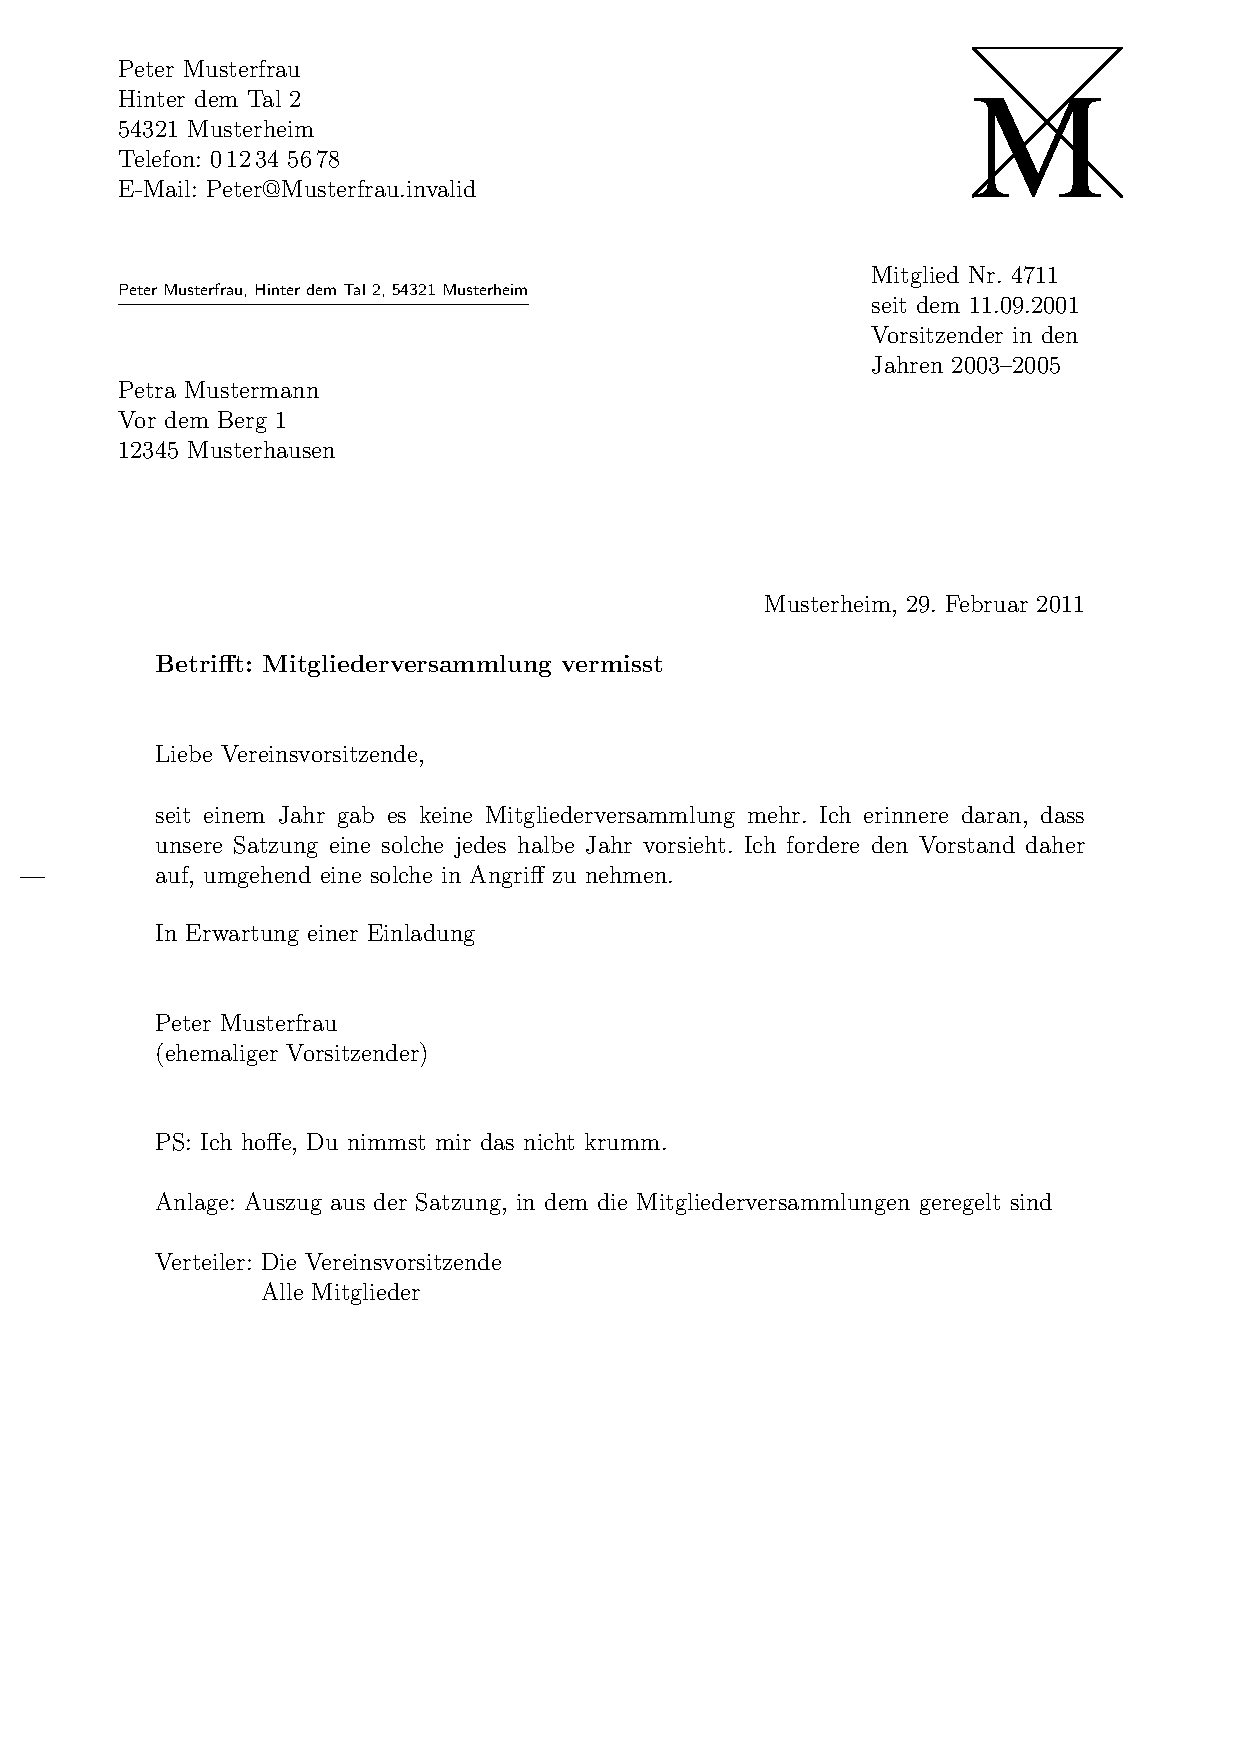
\includegraphics[width=.4\textwidth]{letter-example-23-de}}
    \end{captionbeside}
    \label{fig:\LabelBase.letter-23}
  \end{figure}
\end{Example}

Bitte\textnote{Achtung!} beachten Sie, dass im Beispiel in der Bankverbindung
der Datei \File{ich.lco} für »ß« die \TeX-Schreibweise »\Macro{ss}« verwendet
wurde. Dies hat seinen Grund darin, dass während des Ladens der Klasse weder
ein Paket zur Sprachumschaltung, beispielsweise für die neue, deutsche
Rechtschreibung mit \Macro{usepackage}\POParameter{ngerman}\PParameter{babel},
noch bei älteren \LaTeX-Versionen ein Paket für die Eingabecodierung,
beispielsweise mit \Macro{usepackage}\POParameter{utf8}\PParameter{inputenc}
für moderne Editoren, geladen ist. Wird mit Sicherheit eine \LaTeX-Version ab
April~2018 verwendet und wird die \File{lco}-Datei UTF-8 codiert, so können
Umlaute und Sonderzeichen natürlich auch direkt eingegeben werden.

In \autoref{tab:lcoFiles} finden Sie eine Liste aller vordefinierten
\File{lco}-Dateien. Falls\textnote{Achtung!} Sie einen Drucker verwenden, der
einen sehr großen unbedruckbaren Rand links oder rechts besitzt, werden Sie
mit der Option \Option{SN}\IndexOption{SN} möglicherweise Probleme
bekommen. Da die Schweizer Norm SN~101\,130 vorsieht, dass das Adressfeld
8\Unit{mm} vom rechten Papierrand gesetzt wird, werden bei Schweizer Briefen
auch die Kopfzeile und die Absenderergänzung mit einem entsprechend geringen
Abstand zum Papierrand gesetzt. Dies betrifft ebenfalls die Geschäftszeile bei
der Einstellung
\OptionValueRef{\LabelBase}{refline}{wide}%
\IndexOption{refline~=\textKValue{wide}}
(siehe \autoref{sec:\LabelBase.firstpage},
\DescPageRef{\LabelBase.option.refline}). Sollten\textnote{Tipp!} Sie damit
ein Problem haben, erstellen Sie sich eine eigene \File{lco}-Datei, die
zunächst \Option{SN} lädt und in der
\DescRef{\LabelBase.plength.toaddrhpos}\IndexPLength{toaddrhpos} (siehe
\DescPageRef{\LabelBase.plength.toaddrvpos}) dann auf einen kleineren
Wert gesetzt wird.  Verringern Sie dann außerdem
\DescRef{\LabelBase.plength.toaddrwidth}\IndexPLength{toaddrwidth}
entsprechend.

Die\textnote{Tipp!}\phantomsection\label{tipp:\LabelBase.DIN} \File{lco}-Datei
\File{DIN}\important{\Option{DIN}} wird übrigens immer als erste
\File{lco}-Datei automatisch geladen, damit alle Pseudolängen mehr oder
weniger sinnvoll vordefiniert sind. Es ist daher nicht notwendig diese
voreingestellte Datei selbst zu laden.

Zu den \File{lco}-Dateien \File{DIN5008A}\important{\File{DIN5008A},
  \File{DIN5008B}} und \File{DIN5008B} sei angemerkt, dass die entsprechenden
Vorschriften gewisse Spielräume aufweisen und, wie diversen Anfragen beim
Autor zu entnehmen ist, viele Anwender diese nicht nur auszureizen wünschen,
sondern auch die eine oder andere Abweichung von der Norm bevorzugen. Die
beiden Dateien implementieren jedoch jeweils nur eine einzige Interpretation
der Norm. Der Leser sei daher daran erinnert, dass diese Dateien lediglich als
Vorlagen zu begreifen sind, um das Erstellen eigener angepasster
\File{lco}-Dateien zu erleichtern.%
%
\begin{desclist}
  \renewcommand*{\abovecaptionskipcorrection}{-\normalbaselineskip}%
  \desccaption{%
    Vordefinierte \File{lco}-Dateien\label{tab:lcoFiles}%
  }{%
    Vordefinierte \File{lco}-Dateien (\emph{Fortsetzung})%
  }%
  \oentry{DIN}{%
    \leavevmode%
    \IndexOption[indexmain]{DIN}\IndexFile[indexmain]{DIN.lco}%
    voreingestellter Parametersatz für Briefe im Format A4 nach DIN~676;
    geeignet für Fensterbriefumschläge in den Formaten C4, C5, C6 und C6/5 (C6
    lang)}%
  \oentry{DIN5008A}{%
    \leavevmode%
    \IndexOption[indexmain]{DIN5008A}\IndexFile[indexmain]{DIN5008A.lco}%
    experimenteller Parametersatz für Briefe angelehnt an Variante~A im Format
    A4 nach DIN~5008; geeignet für Fensterbriefumschläge in den Formaten C4,
    C5, C6 und C6/5 (C6 lang)}%
  \oentry{DIN5008B}{%
    \leavevmode%
    \IndexOption[indexmain]{DIN5008B}\IndexFile[indexmain]{DIN5008B.lco}%
    experimenteller Parametersatz für Briefe angelehnt an Variante~B im Format
    A4 nach DIN~5008; geeignet für Fensterbriefumschläge in den Formaten C6
    und C6/5 (C6 lang)}%
  \oentry{DINmtext}{%
    \leavevmode%
    \IndexOption[indexmain]{DINmtext}\IndexFile[indexmain]{DINmtext.lco}%
    Parametersatz für Briefe im Format A4 nach DIN~676, wobei die Alternative
    für mehr Text auf der ersten Briefseite verwendet wird; nur geeignet für
    Fensterbriefumschläge in den Formaten C6 und C6/5 (C6 lang)}%
  \oentry{KakuLL}{%
    \leavevmode%
    \IndexOption[indexmain]{KakuLL}\IndexFile[indexmain]{KakuLL.lco}%
    Parametersatz für japanische Briefe im Format A4; geeignet für japanische
    Fensterbriefumschläge des Typs Kaku A4, bei denen das Fenster in etwa
    90\Unit{mm} breit, 45\Unit{mm} hoch, 25\Unit{mm} vom linken und
    24\Unit{mm} vom oberen Rand entfernt ist (siehe dazu auch \iffree{den
      Anhang der englischen \KOMAScript-Anleitung}{\autoref{cha:japanlco}})}%
  \oentry{KOMAold}{%
    \leavevmode%
    \IndexOption[indexmain]{KOMAold}\IndexFile[indexmain]{KOMAold.lco}%
    \iftrue%
    existiert nur noch aus Kompatibilitätsgründen; die Verwendung wird nicht
    mehr empfohlen%
    \else%
    Parametersatz für Briefe im Format A4 mit Annäherung an das Aussehen von
    Briefen der obsoleten Briefklasse \Class{scrlettr}; geeignet für
    Fensterbriefumschläge in den Formaten C4, C5, C6 und C6/5 (C6 lang); es
    werden einige zusätzliche Anweisungen zur Verbesserung der Kompatibilität
    mit der obsoleten Briefklasse \Class{scrlettr}\IndexClass{scrlettr}
    definiert; \Class{scrlttr2} verhält sich mit dieser \File{lco}-Datei
    möglicherweise nicht genau wie bei Verwendung der übrigen
    \File{lco}-Dateien%
    \fi }%
  \oentry{NF}{%
    \leavevmode%
    \IndexOption[indexmain]{NF}\IndexFile[indexmain]{NF.lco}%
    Parametersatz für französische Briefe nach NF~Z~11-001; geeignet für
    Fensterbriefumschläge im Format DL (110\Unit{mm} auf 220\Unit{mm}) mit
    einem Fenster von 45\Unit{mm} Breite und 100\Unit{mm} Höhe ca. jeweils
    20\Unit{mm} entfernt vom rechten unteren Rand; diese Datei wurde
    ursprünglich von Jean-Marie Pacquet entwickelt, der auf \cite{www:NF.lco}
    neben einer Erweiterung auch eine LyX-Einbindung bereitstellt.}%
  \oentry{NipponEH}{%
    \leavevmode%
    \IndexOption[indexmain]{NipponEH}\IndexFile[indexmain]{NipponEH.lco}%
    Parametersatz für japanische Briefe im Format A4; geeignet für japanische
    Fensterbriefumschläge der Typen Chou oder You 3 oder 4, bei denen das
    Fenster in etwa 90\Unit{mm} breit, 55\Unit{mm} hoch, 22\Unit{mm} vom
    linken und 12\Unit{mm} vom oberen Rand entfernt ist (siehe dazu auch
    \iffree{den Anhang der englischen
      \KOMAScript-Anleitung}{\autoref{cha:japanlco}})}%
  \oentry{NipponEL}{%
    \leavevmode%
    \IndexOption[indexmain]{NipponEL}\IndexFile[indexmain]{NipponEL.lco}%
    Parametersatz für japanische Briefe im Format A4; geeignet für japanische
    Fensterbriefumschläge der Typen Chou oder You 3 oder 4, bei denen das
    Fenster in etwa 90\Unit{mm} breit, 45\Unit{mm} hoch, 22\Unit{mm} vom
    linken und 12\Unit{mm} vom oberen Rand entfernt ist (siehe dazu auch
    \iffree{den Anhang der englischen
      \KOMAScript-Anleitung}{\autoref{cha:japanlco}})}%
  \oentry{NipponLH}{%
    \leavevmode%
    \IndexOption[indexmain]{NipponLH}\IndexFile[indexmain]{NipponLH.lco}%
    Parametersatz für japanische Briefe im Format A4; geeignet für japanische
    Fensterbriefumschläge der Typen Chou oder You 3 oder 4, bei denen das
    Fenster in etwa 90\Unit{mm} breit, 55\Unit{mm} hoch, 25\Unit{mm} vom
    linken und 12\Unit{mm} vom oberen Rand entfernt ist (siehe dazu auch
    \iffree{den Anhang der englischen
      \KOMAScript-Anleitung}{\autoref{cha:japanlco}})}%
  \oentry{NipponLL}{%
    \leavevmode%
    \IndexOption[indexmain]{NipponLL}\IndexFile[indexmain]{NipponLL.lco}%
    Parametersatz für japanische Briefe im Format A4; geeignet für japanische
    Fensterbriefumschläge der Typen Chou oder You 3 oder 4, bei denen das
    Fenster in etwa 90\Unit{mm} breit, 45\Unit{mm} hoch, 25\Unit{mm} vom
    linken und 12\Unit{mm} vom oberen Rand entfernt ist (siehe dazu auch
    \iffree{den Anhang der englischen
      \KOMAScript-Anleitung}{\autoref{cha:japanlco}})}%
  \oentry{NipponRL}{%
    \leavevmode%
    \IndexOption[indexmain]{NipponRL}\IndexFile[indexmain]{NipponRL.lco}%
    Parametersatz für japanische Briefe im Format A4; geeignet für japanische
    Fensterbriefumschläge der Typen Chou oder You 3 oder 4, bei denen das
    Fenster in etwa 90\Unit{mm} breit, 45\Unit{mm} hoch, 22\Unit{mm} vom
    rechten und 28\Unit{mm} vom oberen Rand entfernt ist (siehe dazu auch
    \iffree{den Anhang der englischen
      \KOMAScript-Anleitung}{\autoref{cha:japanlco}})}%
  \oentry{SN}{%
    \leavevmode%
    \IndexOption[indexmain]{SN}\IndexFile[indexmain]{SN.lco}%
    Parametersatz für Schweizer Briefe nach SN~010\,130 mit Anschrift rechts;
    geeignet für Schweizer Fensterbriefumschläge in den Formaten C4, C5, C6
    und C6/5 (C6 lang)}%
  \oentry{SNleft}{%
    \leavevmode%
    \IndexOption[indexmain]{SNleft}\IndexFile[indexmain]{SNleft.lco}%
    Parametersatz für Schweizer Briefe mit Anschrift links; geeignet für
    Schweizer Fensterbriefumschläge mit dem Fenster links in den Formaten C4,
    C5, C6 und C6/5 (C6 lang)}%
  \oentry{UScommercial9}{%
    \leavevmode%
    \IndexOption[indexmain]{UScommercial9}%
    \IndexFile[indexmain]{UScommercial9.lco}%
    Parametersatz für US-amerikanische Briefe im Format letter; geeignet für
    US-amerikanische Fensterbriefumschläge der Größe \emph{commercial~No.\,9}
    mit einem Anschriftfenster der Breite 4\,1/2\Unit{in} und Höhe
    1\,1/8\Unit{in} an einer Position 7/8\Unit{in} von links und 1/2\Unit{in}
    von unten ohne Rücksendeadresse im Fenster; bei Faltung zunächst an der
    Mittelmarke und dann an der oberen Faltmarke kann auch Papier im Format
    legal verwendet werden, führt dann jedoch zu einer Papiergrößen-Warnung}%
  \oentry{UScommercial9DW}{%
    \leavevmode%
    \IndexOption[indexmain]{UScommercial9DW}%
    \IndexFile[indexmain]{UScommercial9DW.lco}%
    Parametersatz für US-amerikanische Briefe im Format letter; geeignet für
    US-amerikanische Fensterbriefumschläge der Größe \emph{commercial~No.\,9}
    mit einem Anschriftfenster der Breite 3\,5/8\Unit{in} und Höhe
    1\,1/8\Unit{in} an einer Position 3/4\Unit{in} von links und 1/2\Unit{in}
    von unten mit einem Absenderfenster der Breite 3\,1/2\Unit{in} und Höhe
    7/8\Unit{in} an einer Position 5/16\Unit{in} von links und 2\,1/2\Unit{in}
    von unten, jedoch ohne Rücksendeadresse im Fenster; bei Faltung zunächst
    an der Mittelmarke und dann an der oberen Faltmarke kann auch Papier im
    Format legal verwendet werden, führt dann jedoch zu einer
    Papiergrößen-Warnung}%
\end{desclist}
%
\EndIndexGroup
%
\EndIndexGroup


\section{Adressdateien und Serienbriefe}
\seclabel{addressFile}%
\BeginIndexGroup
\BeginIndex{}{Adressdatei}\BeginIndex{}{Serienbriefe}%

Als besonders lästig wird bei Briefen immer das Eintippen der Adressen und das
Erstellen von Serienbriefen betrachtet. \KOMAScript{} bietet
hierfür%
\iffalse% Umbruchkorrekturtext
  , wie schon die obsolete Klasse \Class{scrlettr},%
\fi%
\ eine minimalistische Unterstützung.%
\iffalse% Umbruchkorrekturtext
  \ Eine stark verbesserte Serienbrief"|funktion ist bereits seit längerem in
  Planung.%
\fi

\begin{Declaration}
  \Macro{adrentry}\Parameter{Name}\Parameter{Vorname}\Parameter{Adresse}
    \Parameter{Tel.}\Parameter{F1}\Parameter{F2}\Parameter{Kommentar}
    \Parameter{Kürzel}
\end{Declaration}
Mit \Class{scrlttr2} und \Package{scrletter} können
Adressdateien\Index[indexmain]{Adressdatei} ausgewertet werden. Dies ist
beispielsweise für Serienbriefe sehr nützlich. Eine Adressdatei muss
die Endung \File{.adr} haben und besteht aus einer Reihe von
\Macro{adrentry}-Einträgen. Ein solcher Eintrag besteht aus acht
Elementen und kann beispielsweise wie folgt aussehen:
\begin{lstcode}
  \adrentry{Maier}
           {Herbert}
           {Wiesenweg 37\\ 09091 Blumental}
           {0\,23\,34 / 91\,12\,74}
           {Bauunternehmer}
           {}
           {kauft alles}
           {MAIER}
\end{lstcode}
Die Elemente fünf und sechs, \PName{F1} und \PName{F2}, können frei
bestimmt werden. Denkbar wären neben Hinweisen auf das Geschlecht oder
akademische Grade auch der Geburtstag oder das Eintrittsdatum in einen
Verein.  Um das Überschreiben von \TeX- oder \LaTeX-Anweisungen zu
vermeiden, ist es empfehlenswert, für \PName{Kürzel} ausschließlich
Großbuchstaben zu verwenden.

\begin{Example}
  Herr Maier gehört zu Ihren engeren Geschäftspartnern. Da Sie eine
  rege Korrespondenz mit ihm pflegen, ist es Ihnen auf Dauer zu
  mühsam, jedesmal alle Empfängerdaten aufs Neue einzugeben.
  \KOMAScript{} nimmt Ihnen diese Arbeit ab. Angenommen, Sie haben
  Ihre Kundenkontakte in der Datei \File{partner.adr} gespeichert und
  Sie möchten Herrn Maier einen Brief schreiben, dann sparen Sie sich
  viel Tipparbeit, wenn Sie Folgendes eingeben:
\begin{lstcode}
  \input{partner.adr}
  \begin{letter}{\MAIER}
    Der Brief ...
  \end{letter}
\end{lstcode}
  Achten Sie bitte darauf, dass Ihr \TeX-System auch auf die
  \File{.adr}-Dateien zugreifen kann, da sonst eine Fehlermeldung 
  von \Macro{input} verursacht wird. Entweder Sie legen die Brief-
  und Adressdateien im selben Verzeichnis an, oder Sie binden ein
  Adressverzeichnis fest in Ihr \TeX-System ein.
\end{Example}
%
\EndIndexGroup
\vskip-\ht\strutbox% Wegen Beispiel am Ende der Erklärung


\begin{Declaration}
  \Macro{addrentry}\Parameter{Name}\Parameter{Vorname}\Parameter{Adresse}
    \Parameter{Telefon}\Parameter{F1}\Parameter{F2}\Parameter{F3}
    \Parameter{F4}\Parameter{Kürzel}
\end{Declaration}
Bevor Klagen aufkommen, dass insgesamt nur zwei freie Felder zu wenig seien:
\KOMAScript{} verfügt alternativ über die Anweisung \Macro{addrentry}. Mit dem
zusätzlichen »\texttt{d}« im Namen sind hier auch zwei weitere freie Felder
hinzugekommen, dafür ist jedoch der Kommentar entfallen. Ansonsten kann die
Anweisung genau wie \DescRef{\LabelBase.cmd.adrentry} verwendet werden.

In einer \File{adr}-Datei können die beiden Anweisungen
\DescRef{\LabelBase.cmd.adrentry} und \Macro{addrentry} nebeneinander
verwendet werden. Ich\textnote{Achtung!}  weise jedoch darauf hin, dass
Zusatzpakete eventuell nicht auf die Verwendung von \Macro{addrentry} ausgelegt
sind.  Hier muss der Anwender gegebenenfalls selbst entsprechende
Erweiterungen vornehmen.%
%
\EndIndexGroup


Neben dem vereinfachten Zugriff auf Kundendaten können die
\File{.adr}-Dateien auch für Serienbriefe\Index[indexmain]{Serienbriefe}
genutzt werden. So ist es ohne die komplizierte Anbindung an
Datenbanksysteme möglich, solche Massenpostsendungen zu erstellen.
%
\begin{Example}
  Sie wollen einen Serienbrief an alle Mitglieder Ihres
  Anglervereins schicken, um zur nächsten Mitgliederversammlung
  einzuladen.
\begin{lstcode}
  \documentclass{scrlttr2}
  \usepackage[ngerman]{babel}

  \begin{document}
  \renewcommand*{\adrentry}[8]{%
    \begin{letter}{#2 #1\\#3}
      \opening{Liebe Vereinsmitglieder,}
      unsere nächste Mitgliederversammlung findet am 
      Montag, dem 12.~August 2002, statt.
      
      Folgende Punkte müssen besprochen werden...
      \closing{Petri Heil,}
    \end{letter}
  }
  
  \input{mitglieder.adr}
  \end{document}
\end{lstcode}
  Sind in Ihrer \File{adr}-Datei auch
  \DescRef{\LabelBase.cmd.addrentry}-Anweisungen 
  enthalten, müssen Sie dafür eine entsprechende Definition vor dem
  Einladen der Adressdatei ergänzen:
\begin{lstcode}
  \renewcommand*{\addrentry}[9]{%
    \adrentry{#1}{#2}{#3}{#4}{#5}{#6}{#7}{#9}%
  }
\end{lstcode}
  Bei diesem Beispiel wird kein Gebrauch von dem zusätzlichen freien
  Feld gemacht und deshalb \DescRef{\LabelBase.cmd.addrentry} mit Hilfe von
  \DescRef{\LabelBase.cmd.adrentry} definiert.
\end{Example}

Natürlich kann der Brief"|inhalt auch von den Adressatenmerkmalen
abhängig gemacht werden. Als Bedingungsfelder können die frei
bestimmbaren Elemente fünf oder sechs eines
\DescRef{\LabelBase.cmd.adrentry}-Eintrages oder die frei bestimmbaren
Elemente fünf bis acht eines \DescRef{\LabelBase.cmd.addrentry}-Eintrags
genutzt werden.
\begin{Example}
  Angenommen, Sie verwenden das Element fünf, um das Geschlecht eines
  Vereinsmitgliedes zu hinterlegen (\PValue{m/w}) und das sechste
  Element weist auf einen Rückstand der Mitgliedsbeiträge hin. Wollen
  Sie nun alle säumigen Mitglieder anschreiben und persönlich anreden,
  so hilft Ihnen folgendes Beispiel weiter:
\begin{lstcode}
  \renewcommand*{\adrentry}[8]{
    \ifdim #6pt>0pt\relax
      % #6 ist ein Betrag (Gleitkommazahl) größer 0.
      % Es werden also die Säumigen erfasst.
      \begin{letter}{#2 #1\\#3}
        \if #5m \opening{Lieber #2,} \fi
        \if #5w \opening{Liebe #2,} \fi

        Leider mussten wir feststellen, dass du mit 
        der Zahlung deiner Mitgliedsbeiträge im 
        Rückstand bist.

        Wir möchten Dich bitten, den offenen Betrag 
        von #6~EUR auf das Vereinskonto einzuzahlen.
        \closing{Petri Heil,}
      \end{letter}
    \fi
  }
\end{lstcode}
\end{Example}
Es ist also möglich, den Brieftext auf bestimmte Empfängermerkmale
gezielt abzustimmen und so den Eindruck eines persönlichen
Schreibens zu erwecken. Die Anwendungsbreite ist lediglich durch
die maximale Anzahl von zwei freien \DescRef{\LabelBase.cmd.adrentry}-Elementen
beziehungsweise vier freien \DescRef{\LabelBase.cmd.addrentry}-Elementen
begrenzt.


\begin{Declaration}
  \Macro{adrchar}\Parameter{Anfangsbuchstaben}
  \Macro{addrchar}\Parameter{Anfangsbuchstaben}
\end{Declaration}
\Index[indexmain]{Adressverzeichnis}\Index[indexmain]{Telefonliste}%
Es ist auch möglich, die Informationen einer \File{.adr}-Datei in
Adressverzeichnisse oder Telefonlisten umzuwandeln. Sie benötigen dazu
zusätzlich das \Package{adrconv}\IndexPackage{adrconv}-Paket von Axel Kielhorn
(siehe \cite{package:adrconv}). In diesem Paket sind interaktive
\LaTeX-Dokumente enthalten, mit deren Hilfe sehr einfach entsprechende Listen
erstellt werden können.

Damit die Listen alphabetisch sortiert ausgegeben werden, muss bereits die
Adressdatei sortiert gewesen sein. Es empfiehlt sich dabei, vor jedem neuen
Anfangsbuchstaben eine Anweisung \Macro{adrchar} mit diesem Buchstaben als
Argument einzufügen. \Class{scrlttr2} und \Package{scrletter} selbst
ignorieren diese Anweisung ebenso wie \Macro{addrchar}.
%
\begin{Example}
  Angenommen Sie haben folgende, eher winzige Adressdatei, für die ein
  Adressbuch erstellt werden soll:
% In der folgenden lstcode-Umgebung je nach Umbruchbedarf einzelne
% Elemente löschen oder hinzufügen. MICHAEL und GABRIEL sollten jedoch
% erhalten bleiben.
% Umbruchkorrektur: Dies kann noch dazu:
  % \adrentry{Engel}{Raphael}
  %          {Wolke 3b\\12345 Himmelreich}
  %          {000\,01\,02\,05}{}{}{Erzengel}
  %          {RAPHAEL}
  % \adrchar{T}
  % \adrentry{Teufel}{Luzifer}
  %          {Hinter der Flamme 1\\
  %            66666 H\"ollenschlund}
  %          {}{}{}{Gefallener Engel ohne Telefon}
  %          {LUZIFER}
\begin{lstcode}
  \adrchar{E}
  \adrentry{Engel}{Gabriel}
           {Wolke 3\\12345 Himmelreich}
           {000\,01\,02\,03}{}{}{Erzengel}
           {GABRIEL}
  \adrentry{Engel}{Michael}
           {Wolke 3a\\12345 Himmelreich}
           {000\,01\,02\,04}{}{}{Erzengel}
           {MICHAEL}
  \adrchar{K}
  \adrentry{Kohm}{Markus}
           {Freiherr-von-Drais-Stra\ss e 66\\
             68535 Edingen-Neckarhausen}
           {+49~62\,03~1\,??\,??}{}{}
           {\"Uberhaupt kein Engel}
           {KOMA}
\end{lstcode}
  Diese verarbeiten Sie nun unter Verwendung des Dokuments \File{adrdir.tex}
  aus \cite{package:adrconv}. Eine Seite des Ergebnisses sieht dann etwa so aus:
  \begin{center}
    \setlength{\unitlength}{1mm}
    \begin{picture}(80,58)
      \put(0,58){\line(1,0){80}}
      \put(0,3){\line(0,1){55}}
      \put(80,3){\line(0,1){55}}
      \thicklines
      \put(10,43){\line(1,0){60}}
      \put(70,46){\makebox(0,0)[r]{\textsf{\textbf{E}}}}
      \put(10,23){\makebox(0,20)[l]{\parbox{5cm}{\raggedright
            \textsc{Engel}, Gabriel\\\quad\small Wolke 3\\
            \quad 12345 Himmelreich\\
            \quad (Erzengel)}}}
      \put(70,23){\makebox(0,20)[r]{\parbox{2cm}{\raggedright~\\
            \small~\\{\footnotesize GABRIEL}\\000\,01\,02\,03}}}
      \put(10,4){\makebox(0,20)[l]{\parbox{5cm}{\raggedright
            \textsc{Engel}, Michael\\\quad\small Wolke 3a\\
            \quad 12345 Himmelreich\\
            \quad (Erzengel)}}}
      \put(70,4){\makebox(0,20)[r]{\parbox{2cm}{\raggedright~\\
            \small~\\{\footnotesize MICHAEL}\\000\,01\,02\,04}}}
      \qbezier(0,3)(10,6)(40,3)\qbezier(40,3)(60,0)(80,3)
    \end{picture}
  \end{center}
  Dabei wird der Buchstabe in der Kopfzeile von \Macro{adrchar}
  erzeugt, wenn man die Frage »Namen in der Kopfzeile?« verneint. Siehe dazu
  die Definition in \File{adrdir.tex}.%
\end{Example}%

Das Paket \Package{adrconv}\IndexPackage{adrconv} kann auch dazu verwendet
werden, um aus Adressdatenbanken im \BibTeX-Format mit Einträgen wie:
\begin{lstlisting}[morekeywords={@address}]
  @address{HMUS,
     name =      {Hans Mustermann},
     title =     {Mag. art.},
     city =      {Heimstatt},
     zip =       01234,
     country =   {Germany},
     street =    {Mauerstra{\ss}e 1},
     phone =     {01234 / 5 67 89},
     note =      {Alles nur Erfindung},
     key =       {HMUS},
  }
\end{lstlisting}
Adressdateien für die \KOMAScript-Briefklasse oder das \KOMAScript-Briefpaket
zu erzeugen. Näheres zum \Package{adrconv}\IndexPackage{adrconv}-Paket ist der
zugehörigen Anleitung zu entnehmen.%
%
\EndIndexGroup
%
\EndIndexGroup
%
\EndIndexGroup

\endinput

%%% Local Variables: 
%%% mode: latex
%%% TeX-master: "scrguide-de.tex"
%%% coding: utf-8
%%% ispell-local-dictionary: "de_DE"
%%% eval: (flyspell-mode 1)
%%% End: 

%  LocalWords:  Paketoption Satzspiegels Briefklasse Seitenkopf Seitenfuß
%  LocalWords:  Versandart Zentrierung Dokumenttitel Serienbriefen Seitenstil
%  LocalWords:  Dokumentpräambel Grafikpaket Briefbogenfuß Briefbogenfußes
%  LocalWords:  Standardklassen Briefpaket Dokumentteile Briefkontext Torsten
%  LocalWords:  Briefumgebung neckische Briefinhalt Absenderinformationen
%  LocalWords:  Falzmarken Faltmarken Adressfeld Geschäftszeile Feldinhalts
%  LocalWords:  Feldbezeichnung Seitenstilen Paginierung Briefklassenoption
%  LocalWords:  Bedingungsfelder Schriftauswahl Spitzmarke
